\chapter{Investment as a hyperbolic rotation}
\label{chap:finance_rotation}
In this chapter, 

\section{Terminology}
The aim of this research is to refine the way that economic engineering currently deals with financial instruments, primarily fixed-interest assets, but also marketable equity (stocks), derivatives, etc. All of these can be regarded as `investments', for lack of a better word, because they require a \emph{principal}, that is the amount invested, and a certain return that is proportional to the principal. This is why the return is usually expressed as a percentage of the principal, which in the case of debt is the interest rate. The latter contains the word `rate', because it has an inherent timely aspect: interest rates (and returns of investments in general) are associated with a certain `term' or duration over which the return is realized. As such, any type of investment is characterized by three components:
\begin{itemize}
    \item a \emph{principal}, something that is originally invested;
    \item a \emph{return} proportional to the principal;
    \item a \emph{period} over which the return is realized.
\end{itemize}
In the world of finance, the principal and return often refer to some amount of money, but that does not necessarily have to be the case. For example, some stocks pay \emph{stock dividends}, which means that dividends take the form of additional stock. Alternatively, one could look outside finance to other factors of production, such as land: a farmer may `invest' a certain amount of land to gain the earnings (crops that grow on it) after the period of one year; of course, the amount of crops grown is proportional to the surface area of the land that the farmer has cultivated.

\section{Reinvestment of earnings}
After the end of the investment period, the investor has two options: either he can spend his earnings, or he can reinvest them; essentially, he starts the next investment period with a higher principal than the first one. This reinvestment of capital is a crucial concept in the world of finance and is the reason for the existence of compound interest. Indeed, compound interest assumes that one's earnings after one period also bear interest; the so-called \emph{interest on interest}. This can be illustrated by means of the example shown in \cref{fig:compound_interest}. An investor holds a fixed-interest investment with a principal of \$1000 and an interest rate of 5\% annually. After one compounding period, he naturally earns \$50 directly on the principal. As such, his direct earnings, which will be called `yield', now amount to \$50 while the invested `capital' is still \$1000. The next compounding period, however, provided that the investor does not withdraw his earnings from the account, the \$50 generates \$2.5 of interest as well, which are \emph{reinvested}; i.e. they take the form of capital instead of yield. Simultaneously, the investor also keeps the additional benefits from the \$1000 of capital in the form of another \$50 dollars of direct earnings.
\begin{figure}[h]
    \centering
    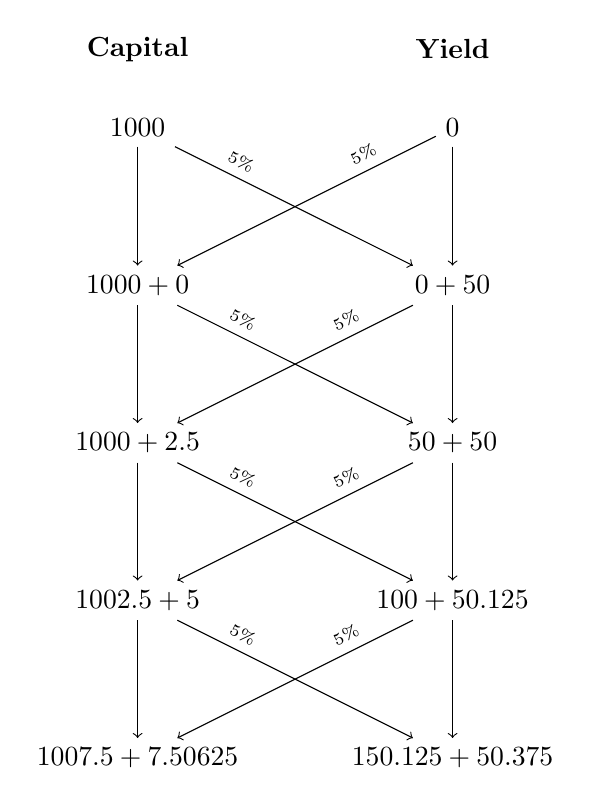
\begin{tikzpicture}
    \path (-2, 1)  node[fill=white, align=center]     {\textbf{Capital}};
    \path (2, 1)   node[fill=white, align=center]     {\textbf{Yield}};
    \path (-2, 0)  node[fill=white, align=center](x1) {1000};
    \path (2, 0)   node[fill=white, align=center](y1) {0};
    \path (-2, -2) node[fill=white, align=center](x2) {\(1000 + 0\)};
    \path (2, -2)  node[fill=white, align=center](y2) {\(0 + 50\)};
    \path (-2, -4) node[fill=white, align=center](x3) {\(1000 + 2.5\)};
    \path (2, -4)  node[fill=white, align=center](y3) {\(50 + 50\)};
    \path (-2, -6) node[fill=white, align=center](x4) {\(1002.5 + 5\)};
    \path (2, -6)  node[fill=white, align=center](y4) {\(100 + 50.125\)};
    \path (-2, -8) node[fill=white, align=center](x5) {\(1007.5 + 7.50625\)};
    \path (2, -8)  node[fill=white, align=center](y5) {\(150.125 + 50.375\)};
    
    \draw[->] (x1) -- (x2);
    \draw[->] (x2) -- (x3);
    \draw[->] (x3) -- (x4);
    \draw[->] (x4) -- (x5);
    
    \draw[->] (y1) -- (y2);
    \draw[->] (y2) -- (y3);
    \draw[->] (y3) -- (y4);
    \draw[->] (y4) -- (y5);
    
    \draw[->] (x1) -- node[near start, sloped, above] {\footnotesize{\(_{5\%}\)}} (y2);
    \draw[->] (x2) -- node[near start, sloped, above] {\footnotesize{\(_{5\%}\)}} (y3);
    \draw[->] (x3) -- node[near start, sloped, above] {\footnotesize{\(_{5\%}\)}} (y4);
    \draw[->] (x4) -- node[near start, sloped, above] {\footnotesize{\(_{5\%}\)}} (y5);
    \draw[->] (y1) -- node[near start, sloped, above] {\footnotesize{\(_{5\%}\)}} (x2);
    \draw[->] (y2) -- node[near start, sloped, above] {\footnotesize{\(_{5\%}\)}} (x3);
    \draw[->] (y3) -- node[near start, sloped, above] {\footnotesize{\(_{5\%}\)}} (x4);
    \draw[->] (y4) -- node[near start, sloped, above] {\footnotesize{\(_{5\%}\)}} (x5);
\end{tikzpicture}

    \caption{A simple example of compound interest with a principal of \$1000 and an interest of 5\%. The direct earnings on the capital are called `yield', while the (re)invested amount is called `capital'.}
    \label{fig:compound_interest}
\end{figure}
This reinvestment of earnings is the driving force behind compound interest: without this step, the investor would end up with \emph{simple interest}, which sees its relative returns essentially decreasing over time. One should, however, be cautious to associate this process exclusively with financial investments; for example, a farmer could use the earnings from his land to buy more land, increase his earnings, use those again to buy even more land, and so forth --- this will again give rise to exponential growth. The farming example makes it quite clear that the object that `generates' the return (capital) is of a very different nature than the return itself (yield). They can be connected through the usage of money as both a unit of account and a medium of exchange, which makes the whole process work \cite{Mankiw2017}. 

Financial investments are arguably the culmination of this concept, since money itself earns money that can be reinvested again instantaneously. Still, the capital-yield distinction remains relevant: for example, companies pay dividends to their shareholders in proportion to the amount of stock they own; the shareholders could then choose to reinvest these earnings in more stock of that (or another) company, increasing their `capital'. An additional example here is stock dividends, which are stocks with dividends that are paid as additional stock --- essentially taking the role of money out of the equation.

\section{The hyperbolic shape of compound interest}
If the numbers from the example in \cref{fig:compound_interest} are plotted against each other, with capital on the horizontal axis and yield on the vertical axis, a hyperbolic shape appears, shown in \cref{fig:hyperbolic_compounding}. Hyperbolae are characterized by the implicit equation 
\begin{equation}
    X^2 - Y^2 = K^2
    \label{eq:hyperbola}
\end{equation}
where \lsymb{$K$}{Original investment} represents the `radius' of the hyperbola, which coincides with the principal amount of the investment. The amount of capital and yield accumulated at a certain time is then on the \lsymb{$X$}{Capital} and \lsymb{$Y$}{Yield}-axis respectively. However, as \cref{fig:hyperbolic_compounding} demonstrates, the shape arising from the example is not quite hyperbolic, since it essentially lags behind the real hyperbola of that radius.
\begin{figure}[h!]
    \centering
    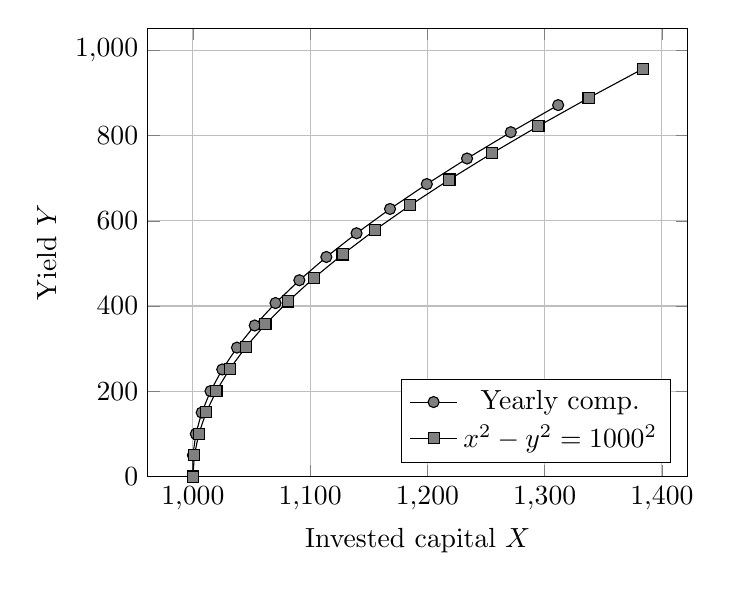
\begin{tikzpicture}[scale=1]
    \begin{axis}[
        xlabel={Invested capital $X$},
        ylabel={Yield $Y$},
        grid,
        cycle list name= black white,
        legend pos = south east,
        ymin = 0,
    ]
        \addplot coordinates {
                    (1000   ,  0     )
                    (1000   ,  50     )
                    (1002.5,  100    )
                    (1007.5,  150.125)
                    (1015.01,  200.5 )
                    (1025.03,  251.25)
                    (1037.59,  302.502)
                    (1052.72,  354.382)
                    (1070.44,  407.018)
                    (1090.79,  460.539)
                    (1113.82,  515.079)
                    (1139.57,  570.77)
                    (1168.11,  627.748)
                    (1199.5,  686.154)
                    (1233.8,  746.128)
                    (1271.11,  807.818)
                    (1311.5,  871.374)
                    % (135.507,  93.6949)
                    % (140.192,  100.47)
                    % (145.215,  107.48)
        };
        \addlegendentry{Yearly comp.};
        
        \addplot coordinates {
            (1000., 0.0)
            (1001.2502604383691, 50.020835937655015)
            (1005.0041680558036, 100.16675001984403)
            (1011.2711095766704, 150.56313315161269)
            (1020.0667556190758, 201.336002541094)
            (1031.4130998795731, 252.6123168081683)
            (1045.3385141288605, 304.52029344714266)
            (1061.8778191559855, 357.18972943727195)
            (1081.0723718384547, 410.7523258028155)
            (1102.970168555971, 465.34201693419774)
            (1127.6259652063807, 521.0953054937474)
            (1155.101414123941, 578.1516037434543)
            (1185.4652182422679, 636.6535821482414)
            (1218.793302887456, 696.7475261264401)
            (1255.169005630943, 758.5837018395335)
            (1294.6832846768447, 822.3167319358299)
            (1337.4349463048446, 888.1059821876231)
            (1383.530891937359, 956.1159599886322)
            %(143.30863854487743, 102.65167257081754)
            %(148.62253413851738, 109.94843179306726)
            %(154.30806348152436, 117.52011936438014)
        };
        \addlegendentry{$x^2 - y^2 = 1000^2$};
        
    \end{axis}
\end{tikzpicture}

    \caption{Plot of the numbers from the example in \cref{fig:compound_interest}. The `ideal' hyperbola with the same radius, given by the equation $X^2 - Y^2 = K^2$ is shown as well.}
    \label{fig:hyperbolic_compounding}
\end{figure}
The reason why the `perfect' hyperbola is not recovered in the example is demonstrated as follows. The capital-yield evolution can be modeled as a second-dimensional difference equation like so:
$$ \mqty(X(k+1)\\Y(k+1)) = \mqty(1& r \\ r & 1)\mqty(X(k)\\Y(k))\qq{with }X(0) = K,\, Y(0) = 0 $$
where $X$ denotes capital, $Y$ denotes yield and $r$ is the interest rate. The solution of this autonomous system is given by:
$$ \mqty(X(k)\\Y(k)) = \mqty(1& r \\ r & 1)^k\mqty(\ininv\\0). $$
One can then write $X(k)^2 - Y(k)^2$ in terms of this solution:
$$ X(k)^2 - Y(k)^2 = \mqty(K & 0)\mqty(1& r \\ r & 1)^k\mqty(1 & 0\\0 & -1)\mqty(1& r \\ r & 1)^k\mqty(K\\0).$$
In order to easily evaluate the matrix powers, one can use the eigenvalue decomposition:
with
$$ \mqty(1 & r \\  r & 1)^k = V\Lambda^k V^{-1} \qq{with } V = \mqty(-1 & 1 \\ 1 & 1) \quad \Lambda = \mqty(1 - r & 0\\0 & 1 + r). $$
Straightforward computations then yield:
$$ X(k)^2 - Y(k)^2 = K^2\qty(1 - r^2)^k, $$
which suggests that for reasonably small values of $r$, the compounding process approximates the equation for the hyperbola. One way to achieve this is to compound faster, i.e. to use more periods with a smaller interest, such that $r \mapsto r/n$ and $k \mapsto kn$ for $n \to \infty$. Indeed, 
$$ \lim_{n\to\infty} K^2\qty(1 - \qty(\frac{r}{n})^2)^{kn} = K^2. $$
That is, for infinitely fast compounding, the capital-yield decomposition of compound interest follows a hyperbolic shape.

Another way to view this is to see the difference equation as a sampled version of an underlying continuous system. One can find the continuous-time state-transition matrix by applying the matrix logarithm to its discrete-time counterpart:
    $$ \log \mqty(1 & r \\ r & 1) = 
        \frac{1}{2}\mqty(\log(r + 1) + \log(r - 1) & \log(r + 1) - \log(r - 1)\\
                         \log(r + 1) - \log(r - 1) & \log(r + 1) + \log(r - 1)). $$
This continuous-time state-transition matrix has eigenvalues $\log(1 + r)$ and $\log(1 - r)$, the former of which is the continuous-time equivalent interest rate, or the \emph{force of interest}, $r_c$ \cite{Kellison1991}. From this discussion, one can infer that the discrete compounding process is essentially an approximation of the underlying `ideal' continuous-time process, which is why the rotational analogy will be developed for a continuous compounding scenario; since the discrete-time equivalent may always be obtained by means of sampling.

\section{Conic sections and hyperbolic rotations}
The implicit equation for a hyperbola \cref{eq:hyperbola} is remarkably similar to the one of a circle: the only difference being the minus sign. Indeed, circles and hyperbola are both members of a larger family called conic sections, which play a prominent role in geometry. Conic sections are usually classified based on their eccentricity $e$, for which three general cases can be distinguished:
\begin{itemize}
    \item $0 \leq e < 1$ are \emph{ellipses}, the special case for which $e = 0$ is a circle;
    \item $e = 1$ holds for \emph{parabolae};
    \item $e > 1$ are hyperbolae.
\end{itemize}
The elliptic-parabolic-hyperbolic (EPH) distinction is a common theme within mathematics and in this literature study, as it also applies to surface curvature, which gives rise to elliptic, parabolic, or hyperbolic geometry (the subject of \cref{chap:hyperbolic_geometry}), and the classification of Möbius transformations discussed in \cref{chap:moebius_transforms}.

\citet{Harkin2004} use the conic sections to extend the `classic' trigonometry based on circles (i.e. elliptic curves) to hyperbolic and parabolic trigonometry as well. Associated with each of these types of geometry is also a special number system akin to complex numbers, called double numbers (or hyperbolic numbers) and dual numbers (or parabolic numbers) --- hyperbolic numbers will briefly be explored in \cref{sec:hyperbolic_numbers}. The results of the previous section suggest that hyperbolic trigonometry can be used to describe investment problems: this will be the basis for the \emph{rotational analogy} in economic engineering, which will be introduced in \cref{sec:rotational_analogy}.

\subsection{Hyperbolic angles}
For both circles and hyperbolae, an angle refers to a certain region bounded by the curve at issue. The standard notation for the hyperbolic angle will be \(\zeta\), in accordance with the rapidity from special relativity, which can also be viewed as a hyperbolic angle (cf. \cref{chap:relativity}).
\begin{thmblock}{Hyperbolic sector}
A hyperbolic sector is a region bounded by two lines extending from the origin to each to a point on the (unit) hyperbola, and the graph of the hyperbola itself. 
\end{thmblock}
Clearly, hyperbolic sectors are entirely analogous to their `traditional' circular cousins. Fixing one of the rays to the \(x\)-axis, one can define the corresponding hyperbolic angle:
\begin{thmblock}{Hyperbolic angle}
A hyperbolic angle corresponding to a point \(A\) is defined as twice the area of the hyperbolic sector based on the point \(A\) and the intersection point of the unit hyperbola and the \(x\)-axis \((K, 0)\).
\end{thmblock}
\Cref{fig:hyperbolic_angle} visualizes the concept of a hyperbolic angle: the angle $\zeta$ is defined in terms of the unit hyperbola $X^2 - Y^2 = 1$, or the hyperbola with `radius' 1. 
Just like for circles, the hyperbolic angle is defined on the unit hyperbola, but using a special (polar) coordinate set points can be expressed in terms of a radius $K$ and an angle $\zeta$. By allowing the radius \(K\) to be negative, all the points in the disconnected open set bounded by \(y = x\) and \(y = -x\) can be identified with a unique radius \(K\) and hyperbolic angle \(\zeta\). This is somewhat similar to polar coordinates, which is why these coordinates will be referred to as `hyperbolic polar coordinates'. These coordinates are interesting because they allow to express investments in a very natural way in terms of their principal and realized return. 
\begin{figure}[ht!]
    \centering
    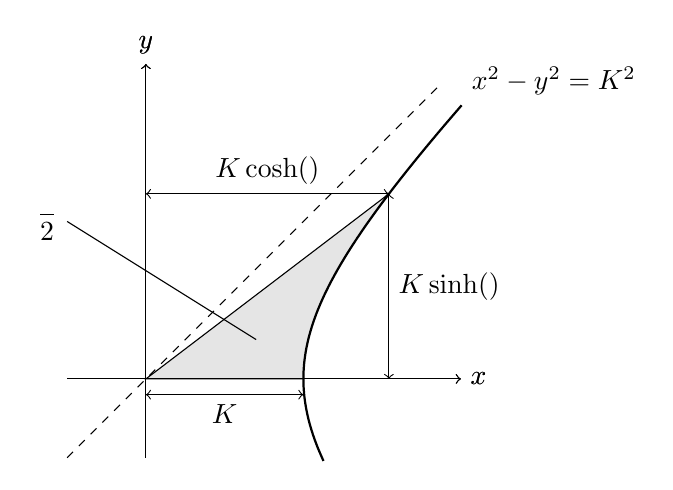
\begin{tikzpicture}[scale=2]
    \draw[->] (-0.5, 0) -- (2, 0) node[right] {$x$};
    \draw[->] (0, -0.5) -- (0, 2) node[above] {$y$};
    \filldraw[fill=gray!20] (0, 0) -- (1, 0) -- (1.54308, 1.1752) -- cycle;
    \filldraw[domain=-0.5:1.32, smooth, variable=\x, thick, fill=white] plot ({cosh(\x)}, {sinh(\x)}) node[anchor=south west] {$x^2 - y^2 = K^2$};
    \draw[dashed] (-0.5, -0.5) -- (1.85, 1.85);
    \draw[->] (-0.5, 0) -- (2, 0) node[right] {$x$};
    \draw[->] (0, -0.5) -- (0, 2) node[above] {$y$};
    \draw (-0.5, 1) node[right, anchor=east] {$\displaystyle\frac{\han}{2}$} -- (0.7, 0.25);
    \draw[<->] (0, 1.1752) -- (1.54308, 1.1752) node[pos=0.5, anchor=south] {$K\cosh(\han)$}; 
    \draw[<->] (1.54308, 0) -- (1.54308, 1.1752) node[pos=0.5, anchor=west] {$K\sinh(\han)$}; 
    \draw[<->] (0, -0.1) -- (1, -0.1) node[pos=0.5, anchor=north] {$K$};
\end{tikzpicture}
    \caption{Illustration of a hyperbolic angle along the unit hyperbola, with projection on the axes using the hyperbolic sine and cosine.}
    \label{fig:hyperbolic_angle}
\end{figure}

The preceding discussion suggests that hyperbolic polar coordinates do \emph{not} provide coordinates for the entire plane like regular polar coordinates do. Indeed, the mapping defined by the coordinate functions from the \(K-\zeta\) space to the \(x\)-\(y\) space is neither injective nor surjective: its image is the disconnected open set bounded by the lines \(y = x\) and \(y = -x\) (not surjective), and the entire line \(K = 0\) in the \(K-\zeta\) plane is mapped to the origin in the \(x-y\) plane (not injective). As such, one can obtain a bijection by disregarding the degenerate cases for which \(K = 0\) and restricting the co-domain of the mapping to the set \(\qty{(x, y) \in \real^2: \abs{x} > \abs{y}}\). The action of the mapping is illustrated by \cref{fig:polar_coords}.
\begin{figure}[ht]
    \centering
    % This file was created by matlab2tikz.
%
%The latest updates can be retrieved from
%  http://www.mathworks.com/matlabcentral/fileexchange/22022-matlab2tikz-matlab2tikz
%where you can also make suggestions and rate matlab2tikz.
%
\definecolor{mycolor1}{rgb}{0.23922,0.59608,0.87059}%
\definecolor{mycolor2}{rgb}{0.84706,0.29020,0.23137}%
\definecolor{mycolor3}{rgb}{0.18039,0.80000,0.44314}%
\definecolor{mycolor4}{rgb}{0.94510,0.76863,0.05882}%
%
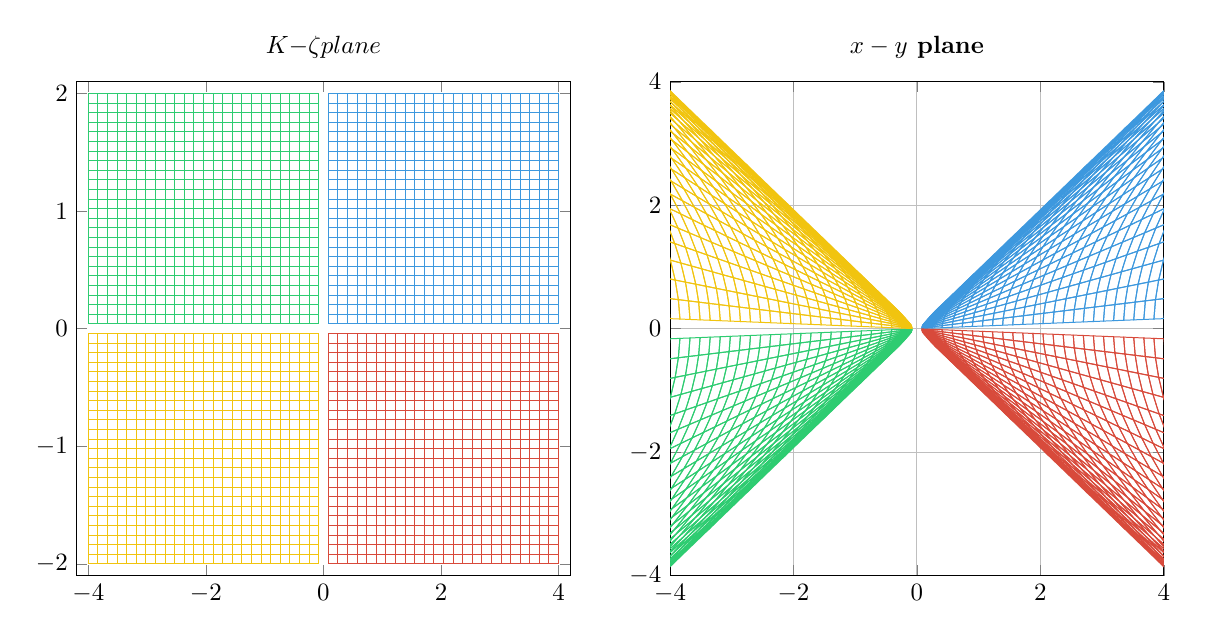
\begin{tikzpicture}[scale=0.9]

\begin{axis}[%
width=2.743in,
height=2.743in,
at={(0.483in,0.269in)},
scale only axis,
xmin=-4.2,
xmax=4.2,
ymin=-2.1,
ymax=2.1,
axis background/.style={fill=white},
title style={font=\bfseries},
title={$\text{K-}\zeta\text{ plane}$}
]

\addplot[%
surf,
fill=white, faceted color=mycolor1, colormap={mymap}{[1pt] rgb(0pt)=(0.2422,0.1504,0.6603); rgb(1pt)=(0.2444,0.1534,0.6728); rgb(2pt)=(0.2464,0.1569,0.6847); rgb(3pt)=(0.2484,0.1607,0.6961); rgb(4pt)=(0.2503,0.1648,0.7071); rgb(5pt)=(0.2522,0.1689,0.7179); rgb(6pt)=(0.254,0.1732,0.7286); rgb(7pt)=(0.2558,0.1773,0.7393); rgb(8pt)=(0.2576,0.1814,0.7501); rgb(9pt)=(0.2594,0.1854,0.761); rgb(11pt)=(0.2628,0.1932,0.7828); rgb(12pt)=(0.2645,0.1972,0.7937); rgb(13pt)=(0.2661,0.2011,0.8043); rgb(14pt)=(0.2676,0.2052,0.8148); rgb(15pt)=(0.2691,0.2094,0.8249); rgb(16pt)=(0.2704,0.2138,0.8346); rgb(17pt)=(0.2717,0.2184,0.8439); rgb(18pt)=(0.2729,0.2231,0.8528); rgb(19pt)=(0.274,0.228,0.8612); rgb(20pt)=(0.2749,0.233,0.8692); rgb(21pt)=(0.2758,0.2382,0.8767); rgb(22pt)=(0.2766,0.2435,0.884); rgb(23pt)=(0.2774,0.2489,0.8908); rgb(24pt)=(0.2781,0.2543,0.8973); rgb(25pt)=(0.2788,0.2598,0.9035); rgb(26pt)=(0.2794,0.2653,0.9094); rgb(27pt)=(0.2798,0.2708,0.915); rgb(28pt)=(0.2802,0.2764,0.9204); rgb(29pt)=(0.2806,0.2819,0.9255); rgb(30pt)=(0.2809,0.2875,0.9305); rgb(31pt)=(0.2811,0.293,0.9352); rgb(32pt)=(0.2813,0.2985,0.9397); rgb(33pt)=(0.2814,0.304,0.9441); rgb(34pt)=(0.2814,0.3095,0.9483); rgb(35pt)=(0.2813,0.315,0.9524); rgb(36pt)=(0.2811,0.3204,0.9563); rgb(37pt)=(0.2809,0.3259,0.96); rgb(38pt)=(0.2807,0.3313,0.9636); rgb(39pt)=(0.2803,0.3367,0.967); rgb(40pt)=(0.2798,0.3421,0.9702); rgb(41pt)=(0.2791,0.3475,0.9733); rgb(42pt)=(0.2784,0.3529,0.9763); rgb(43pt)=(0.2776,0.3583,0.9791); rgb(44pt)=(0.2766,0.3638,0.9817); rgb(45pt)=(0.2754,0.3693,0.984); rgb(46pt)=(0.2741,0.3748,0.9862); rgb(47pt)=(0.2726,0.3804,0.9881); rgb(48pt)=(0.271,0.386,0.9898); rgb(49pt)=(0.2691,0.3916,0.9912); rgb(50pt)=(0.267,0.3973,0.9924); rgb(51pt)=(0.2647,0.403,0.9935); rgb(52pt)=(0.2621,0.4088,0.9946); rgb(53pt)=(0.2591,0.4145,0.9955); rgb(54pt)=(0.2556,0.4203,0.9965); rgb(55pt)=(0.2517,0.4261,0.9974); rgb(56pt)=(0.2473,0.4319,0.9983); rgb(57pt)=(0.2424,0.4378,0.9991); rgb(58pt)=(0.2369,0.4437,0.9996); rgb(59pt)=(0.2311,0.4497,0.9995); rgb(60pt)=(0.225,0.4559,0.9985); rgb(61pt)=(0.2189,0.462,0.9968); rgb(62pt)=(0.2128,0.4682,0.9948); rgb(63pt)=(0.2066,0.4743,0.9926); rgb(64pt)=(0.2006,0.4803,0.9906); rgb(65pt)=(0.195,0.4861,0.9887); rgb(66pt)=(0.1903,0.4919,0.9867); rgb(67pt)=(0.1869,0.4975,0.9844); rgb(68pt)=(0.1847,0.503,0.9819); rgb(69pt)=(0.1831,0.5084,0.9793); rgb(70pt)=(0.1818,0.5138,0.9766); rgb(71pt)=(0.1806,0.5191,0.9738); rgb(72pt)=(0.1795,0.5244,0.9709); rgb(73pt)=(0.1785,0.5296,0.9677); rgb(74pt)=(0.1778,0.5349,0.9641); rgb(75pt)=(0.1773,0.5401,0.9602); rgb(76pt)=(0.1768,0.5452,0.956); rgb(77pt)=(0.1764,0.5504,0.9516); rgb(78pt)=(0.1755,0.5554,0.9473); rgb(79pt)=(0.174,0.5605,0.9432); rgb(80pt)=(0.1716,0.5655,0.9393); rgb(81pt)=(0.1686,0.5705,0.9357); rgb(82pt)=(0.1649,0.5755,0.9323); rgb(83pt)=(0.161,0.5805,0.9289); rgb(84pt)=(0.1573,0.5854,0.9254); rgb(85pt)=(0.154,0.5902,0.9218); rgb(86pt)=(0.1513,0.595,0.9182); rgb(87pt)=(0.1492,0.5997,0.9147); rgb(88pt)=(0.1475,0.6043,0.9113); rgb(89pt)=(0.1461,0.6089,0.908); rgb(90pt)=(0.1446,0.6135,0.905); rgb(91pt)=(0.1429,0.618,0.9022); rgb(92pt)=(0.1408,0.6226,0.8998); rgb(93pt)=(0.1383,0.6272,0.8975); rgb(94pt)=(0.1354,0.6317,0.8953); rgb(95pt)=(0.1321,0.6363,0.8932); rgb(96pt)=(0.1288,0.6408,0.891); rgb(97pt)=(0.1253,0.6453,0.8887); rgb(98pt)=(0.1219,0.6497,0.8862); rgb(99pt)=(0.1185,0.6541,0.8834); rgb(100pt)=(0.1152,0.6584,0.8804); rgb(101pt)=(0.1119,0.6627,0.877); rgb(102pt)=(0.1085,0.6669,0.8734); rgb(103pt)=(0.1048,0.671,0.8695); rgb(104pt)=(0.1009,0.675,0.8653); rgb(105pt)=(0.0964,0.6789,0.8609); rgb(106pt)=(0.0914,0.6828,0.8562); rgb(107pt)=(0.0855,0.6865,0.8513); rgb(108pt)=(0.0789,0.6902,0.8462); rgb(109pt)=(0.0713,0.6938,0.8409); rgb(110pt)=(0.0628,0.6972,0.8355); rgb(111pt)=(0.0535,0.7006,0.8299); rgb(112pt)=(0.0433,0.7039,0.8242); rgb(113pt)=(0.0328,0.7071,0.8183); rgb(114pt)=(0.0234,0.7103,0.8124); rgb(115pt)=(0.0155,0.7133,0.8064); rgb(116pt)=(0.0091,0.7163,0.8003); rgb(117pt)=(0.0046,0.7192,0.7941); rgb(118pt)=(0.0019,0.722,0.7878); rgb(119pt)=(0.0009,0.7248,0.7815); rgb(120pt)=(0.0018,0.7275,0.7752); rgb(121pt)=(0.0046,0.7301,0.7688); rgb(122pt)=(0.0094,0.7327,0.7623); rgb(123pt)=(0.0162,0.7352,0.7558); rgb(124pt)=(0.0253,0.7376,0.7492); rgb(125pt)=(0.0369,0.74,0.7426); rgb(126pt)=(0.0504,0.7423,0.7359); rgb(127pt)=(0.0638,0.7446,0.7292); rgb(128pt)=(0.077,0.7468,0.7224); rgb(129pt)=(0.0899,0.7489,0.7156); rgb(130pt)=(0.1023,0.751,0.7088); rgb(131pt)=(0.1141,0.7531,0.7019); rgb(132pt)=(0.1252,0.7552,0.695); rgb(133pt)=(0.1354,0.7572,0.6881); rgb(134pt)=(0.1448,0.7593,0.6812); rgb(135pt)=(0.1532,0.7614,0.6741); rgb(136pt)=(0.1609,0.7635,0.6671); rgb(137pt)=(0.1678,0.7656,0.6599); rgb(138pt)=(0.1741,0.7678,0.6527); rgb(139pt)=(0.1799,0.7699,0.6454); rgb(140pt)=(0.1853,0.7721,0.6379); rgb(141pt)=(0.1905,0.7743,0.6303); rgb(142pt)=(0.1954,0.7765,0.6225); rgb(143pt)=(0.2003,0.7787,0.6146); rgb(144pt)=(0.2061,0.7808,0.6065); rgb(145pt)=(0.2118,0.7828,0.5983); rgb(146pt)=(0.2178,0.7849,0.5899); rgb(147pt)=(0.2244,0.7869,0.5813); rgb(148pt)=(0.2318,0.7887,0.5725); rgb(149pt)=(0.2401,0.7905,0.5636); rgb(150pt)=(0.2491,0.7922,0.5546); rgb(151pt)=(0.2589,0.7937,0.5454); rgb(152pt)=(0.2695,0.7951,0.536); rgb(153pt)=(0.2809,0.7964,0.5266); rgb(154pt)=(0.2929,0.7975,0.517); rgb(155pt)=(0.3052,0.7985,0.5074); rgb(156pt)=(0.3176,0.7994,0.4975); rgb(157pt)=(0.3301,0.8002,0.4876); rgb(158pt)=(0.3424,0.8009,0.4774); rgb(159pt)=(0.3548,0.8016,0.4669); rgb(160pt)=(0.3671,0.8021,0.4563); rgb(161pt)=(0.3795,0.8026,0.4454); rgb(162pt)=(0.3921,0.8029,0.4344); rgb(163pt)=(0.405,0.8031,0.4233); rgb(164pt)=(0.4184,0.803,0.4122); rgb(165pt)=(0.4322,0.8028,0.4013); rgb(166pt)=(0.4463,0.8024,0.3904); rgb(167pt)=(0.4608,0.8018,0.3797); rgb(168pt)=(0.4753,0.8011,0.3691); rgb(169pt)=(0.4899,0.8002,0.3586); rgb(170pt)=(0.5044,0.7993,0.348); rgb(171pt)=(0.5187,0.7982,0.3374); rgb(172pt)=(0.5329,0.797,0.3267); rgb(173pt)=(0.547,0.7957,0.3159); rgb(175pt)=(0.5748,0.7929,0.2941); rgb(176pt)=(0.5886,0.7913,0.2833); rgb(177pt)=(0.6024,0.7896,0.2726); rgb(178pt)=(0.6161,0.7878,0.2622); rgb(179pt)=(0.6297,0.7859,0.2521); rgb(180pt)=(0.6433,0.7839,0.2423); rgb(181pt)=(0.6567,0.7818,0.2329); rgb(182pt)=(0.6701,0.7796,0.2239); rgb(183pt)=(0.6833,0.7773,0.2155); rgb(184pt)=(0.6963,0.775,0.2075); rgb(185pt)=(0.7091,0.7727,0.1998); rgb(186pt)=(0.7218,0.7703,0.1924); rgb(187pt)=(0.7344,0.7679,0.1852); rgb(188pt)=(0.7468,0.7654,0.1782); rgb(189pt)=(0.759,0.7629,0.1717); rgb(190pt)=(0.771,0.7604,0.1658); rgb(191pt)=(0.7829,0.7579,0.1608); rgb(192pt)=(0.7945,0.7554,0.157); rgb(193pt)=(0.806,0.7529,0.1546); rgb(194pt)=(0.8172,0.7505,0.1535); rgb(195pt)=(0.8281,0.7481,0.1536); rgb(196pt)=(0.8389,0.7457,0.1546); rgb(197pt)=(0.8495,0.7435,0.1564); rgb(198pt)=(0.86,0.7413,0.1587); rgb(199pt)=(0.8703,0.7392,0.1615); rgb(200pt)=(0.8804,0.7372,0.165); rgb(201pt)=(0.8903,0.7353,0.1695); rgb(202pt)=(0.9,0.7336,0.1749); rgb(203pt)=(0.9093,0.7321,0.1815); rgb(204pt)=(0.9184,0.7308,0.189); rgb(205pt)=(0.9272,0.7298,0.1973); rgb(206pt)=(0.9357,0.729,0.2061); rgb(207pt)=(0.944,0.7285,0.2151); rgb(208pt)=(0.9523,0.7284,0.2237); rgb(209pt)=(0.9606,0.7285,0.2312); rgb(210pt)=(0.9689,0.7292,0.2373); rgb(211pt)=(0.977,0.7304,0.2418); rgb(212pt)=(0.9842,0.733,0.2446); rgb(213pt)=(0.99,0.7365,0.2429); rgb(214pt)=(0.9946,0.7407,0.2394); rgb(215pt)=(0.9966,0.7458,0.2351); rgb(216pt)=(0.9971,0.7513,0.2309); rgb(217pt)=(0.9972,0.7569,0.2267); rgb(218pt)=(0.9971,0.7626,0.2224); rgb(219pt)=(0.9969,0.7683,0.2181); rgb(220pt)=(0.9966,0.774,0.2138); rgb(221pt)=(0.9962,0.7798,0.2095); rgb(222pt)=(0.9957,0.7856,0.2053); rgb(223pt)=(0.9949,0.7915,0.2012); rgb(224pt)=(0.9938,0.7974,0.1974); rgb(225pt)=(0.9923,0.8034,0.1939); rgb(226pt)=(0.9906,0.8095,0.1906); rgb(227pt)=(0.9885,0.8156,0.1875); rgb(228pt)=(0.9861,0.8218,0.1846); rgb(229pt)=(0.9835,0.828,0.1817); rgb(230pt)=(0.9807,0.8342,0.1787); rgb(231pt)=(0.9778,0.8404,0.1757); rgb(232pt)=(0.9748,0.8467,0.1726); rgb(233pt)=(0.972,0.8529,0.1695); rgb(234pt)=(0.9694,0.8591,0.1665); rgb(235pt)=(0.9671,0.8654,0.1636); rgb(236pt)=(0.9651,0.8716,0.1608); rgb(237pt)=(0.9634,0.8778,0.1582); rgb(238pt)=(0.9619,0.884,0.1557); rgb(239pt)=(0.9608,0.8902,0.1532); rgb(240pt)=(0.9601,0.8963,0.1507); rgb(241pt)=(0.9596,0.9023,0.148); rgb(242pt)=(0.9595,0.9084,0.145); rgb(243pt)=(0.9597,0.9143,0.1418); rgb(244pt)=(0.9601,0.9203,0.1382); rgb(245pt)=(0.9608,0.9262,0.1344); rgb(246pt)=(0.9618,0.932,0.1304); rgb(247pt)=(0.9629,0.9379,0.1261); rgb(248pt)=(0.9642,0.9437,0.1216); rgb(249pt)=(0.9657,0.9494,0.1168); rgb(250pt)=(0.9674,0.9552,0.1116); rgb(251pt)=(0.9692,0.9609,0.1061); rgb(252pt)=(0.9711,0.9667,0.1001); rgb(253pt)=(0.973,0.9724,0.0938); rgb(254pt)=(0.9749,0.9782,0.0872); rgb(255pt)=(0.9769,0.9839,0.0805)}, mesh/rows=25]
table[row sep=crcr, point meta=\thisrow{c}] {%
%
x	y	c\\
0.0816326530612245	0.0408163265306122	-1\\
0.0816326530612245	0.122448979591837	-1\\
0.0816326530612245	0.204081632653061	-1\\
0.0816326530612245	0.285714285714286	-1\\
0.0816326530612245	0.36734693877551	-1\\
0.0816326530612245	0.448979591836735	-1\\
0.0816326530612245	0.530612244897959	-1\\
0.0816326530612245	0.612244897959184	-1\\
0.0816326530612245	0.693877551020408	-1\\
0.0816326530612245	0.775510204081633	-1\\
0.0816326530612245	0.857142857142857	-1\\
0.0816326530612245	0.938775510204082	-1\\
0.0816326530612245	1.02040816326531	-1\\
0.0816326530612245	1.10204081632653	-1\\
0.0816326530612245	1.18367346938776	-1\\
0.0816326530612245	1.26530612244898	-1\\
0.0816326530612245	1.3469387755102	-1\\
0.0816326530612245	1.42857142857143	-1\\
0.0816326530612245	1.51020408163265	-1\\
0.0816326530612245	1.59183673469388	-1\\
0.0816326530612245	1.6734693877551	-1\\
0.0816326530612245	1.75510204081633	-1\\
0.0816326530612245	1.83673469387755	-1\\
0.0816326530612245	1.91836734693878	-1\\
0.0816326530612245	2	-1\\
0.244897959183673	0.0408163265306122	-1\\
0.244897959183673	0.122448979591837	-1\\
0.244897959183673	0.204081632653061	-1\\
0.244897959183673	0.285714285714286	-1\\
0.244897959183673	0.36734693877551	-1\\
0.244897959183673	0.448979591836735	-1\\
0.244897959183673	0.530612244897959	-1\\
0.244897959183673	0.612244897959184	-1\\
0.244897959183673	0.693877551020408	-1\\
0.244897959183673	0.775510204081633	-1\\
0.244897959183673	0.857142857142857	-1\\
0.244897959183673	0.938775510204082	-1\\
0.244897959183673	1.02040816326531	-1\\
0.244897959183673	1.10204081632653	-1\\
0.244897959183673	1.18367346938776	-1\\
0.244897959183673	1.26530612244898	-1\\
0.244897959183673	1.3469387755102	-1\\
0.244897959183673	1.42857142857143	-1\\
0.244897959183673	1.51020408163265	-1\\
0.244897959183673	1.59183673469388	-1\\
0.244897959183673	1.6734693877551	-1\\
0.244897959183673	1.75510204081633	-1\\
0.244897959183673	1.83673469387755	-1\\
0.244897959183673	1.91836734693878	-1\\
0.244897959183673	2	-1\\
0.408163265306122	0.0408163265306122	-1\\
0.408163265306122	0.122448979591837	-1\\
0.408163265306122	0.204081632653061	-1\\
0.408163265306122	0.285714285714286	-1\\
0.408163265306122	0.36734693877551	-1\\
0.408163265306122	0.448979591836735	-1\\
0.408163265306122	0.530612244897959	-1\\
0.408163265306122	0.612244897959184	-1\\
0.408163265306122	0.693877551020408	-1\\
0.408163265306122	0.775510204081633	-1\\
0.408163265306122	0.857142857142857	-1\\
0.408163265306122	0.938775510204082	-1\\
0.408163265306122	1.02040816326531	-1\\
0.408163265306122	1.10204081632653	-1\\
0.408163265306122	1.18367346938776	-1\\
0.408163265306122	1.26530612244898	-1\\
0.408163265306122	1.3469387755102	-1\\
0.408163265306122	1.42857142857143	-1\\
0.408163265306122	1.51020408163265	-1\\
0.408163265306122	1.59183673469388	-1\\
0.408163265306122	1.6734693877551	-1\\
0.408163265306122	1.75510204081633	-1\\
0.408163265306122	1.83673469387755	-1\\
0.408163265306122	1.91836734693878	-1\\
0.408163265306122	2	-1\\
0.571428571428571	0.0408163265306122	-1\\
0.571428571428571	0.122448979591837	-1\\
0.571428571428571	0.204081632653061	-1\\
0.571428571428571	0.285714285714286	-1\\
0.571428571428571	0.36734693877551	-1\\
0.571428571428571	0.448979591836735	-1\\
0.571428571428571	0.530612244897959	-1\\
0.571428571428571	0.612244897959184	-1\\
0.571428571428571	0.693877551020408	-1\\
0.571428571428571	0.775510204081633	-1\\
0.571428571428571	0.857142857142857	-1\\
0.571428571428571	0.938775510204082	-1\\
0.571428571428571	1.02040816326531	-1\\
0.571428571428571	1.10204081632653	-1\\
0.571428571428571	1.18367346938776	-1\\
0.571428571428571	1.26530612244898	-1\\
0.571428571428571	1.3469387755102	-1\\
0.571428571428571	1.42857142857143	-1\\
0.571428571428571	1.51020408163265	-1\\
0.571428571428571	1.59183673469388	-1\\
0.571428571428571	1.6734693877551	-1\\
0.571428571428571	1.75510204081633	-1\\
0.571428571428571	1.83673469387755	-1\\
0.571428571428571	1.91836734693878	-1\\
0.571428571428571	2	-1\\
0.73469387755102	0.0408163265306122	-1\\
0.73469387755102	0.122448979591837	-1\\
0.73469387755102	0.204081632653061	-1\\
0.73469387755102	0.285714285714286	-1\\
0.73469387755102	0.36734693877551	-1\\
0.73469387755102	0.448979591836735	-1\\
0.73469387755102	0.530612244897959	-1\\
0.73469387755102	0.612244897959184	-1\\
0.73469387755102	0.693877551020408	-1\\
0.73469387755102	0.775510204081633	-1\\
0.73469387755102	0.857142857142857	-1\\
0.73469387755102	0.938775510204082	-1\\
0.73469387755102	1.02040816326531	-1\\
0.73469387755102	1.10204081632653	-1\\
0.73469387755102	1.18367346938776	-1\\
0.73469387755102	1.26530612244898	-1\\
0.73469387755102	1.3469387755102	-1\\
0.73469387755102	1.42857142857143	-1\\
0.73469387755102	1.51020408163265	-1\\
0.73469387755102	1.59183673469388	-1\\
0.73469387755102	1.6734693877551	-1\\
0.73469387755102	1.75510204081633	-1\\
0.73469387755102	1.83673469387755	-1\\
0.73469387755102	1.91836734693878	-1\\
0.73469387755102	2	-1\\
0.897959183673469	0.0408163265306122	-1\\
0.897959183673469	0.122448979591837	-1\\
0.897959183673469	0.204081632653061	-1\\
0.897959183673469	0.285714285714286	-1\\
0.897959183673469	0.36734693877551	-1\\
0.897959183673469	0.448979591836735	-1\\
0.897959183673469	0.530612244897959	-1\\
0.897959183673469	0.612244897959184	-1\\
0.897959183673469	0.693877551020408	-1\\
0.897959183673469	0.775510204081633	-1\\
0.897959183673469	0.857142857142857	-1\\
0.897959183673469	0.938775510204082	-1\\
0.897959183673469	1.02040816326531	-1\\
0.897959183673469	1.10204081632653	-1\\
0.897959183673469	1.18367346938776	-1\\
0.897959183673469	1.26530612244898	-1\\
0.897959183673469	1.3469387755102	-1\\
0.897959183673469	1.42857142857143	-1\\
0.897959183673469	1.51020408163265	-1\\
0.897959183673469	1.59183673469388	-1\\
0.897959183673469	1.6734693877551	-1\\
0.897959183673469	1.75510204081633	-1\\
0.897959183673469	1.83673469387755	-1\\
0.897959183673469	1.91836734693878	-1\\
0.897959183673469	2	-1\\
1.06122448979592	0.0408163265306122	-1\\
1.06122448979592	0.122448979591837	-1\\
1.06122448979592	0.204081632653061	-1\\
1.06122448979592	0.285714285714286	-1\\
1.06122448979592	0.36734693877551	-1\\
1.06122448979592	0.448979591836735	-1\\
1.06122448979592	0.530612244897959	-1\\
1.06122448979592	0.612244897959184	-1\\
1.06122448979592	0.693877551020408	-1\\
1.06122448979592	0.775510204081633	-1\\
1.06122448979592	0.857142857142857	-1\\
1.06122448979592	0.938775510204082	-1\\
1.06122448979592	1.02040816326531	-1\\
1.06122448979592	1.10204081632653	-1\\
1.06122448979592	1.18367346938776	-1\\
1.06122448979592	1.26530612244898	-1\\
1.06122448979592	1.3469387755102	-1\\
1.06122448979592	1.42857142857143	-1\\
1.06122448979592	1.51020408163265	-1\\
1.06122448979592	1.59183673469388	-1\\
1.06122448979592	1.6734693877551	-1\\
1.06122448979592	1.75510204081633	-1\\
1.06122448979592	1.83673469387755	-1\\
1.06122448979592	1.91836734693878	-1\\
1.06122448979592	2	-1\\
1.22448979591837	0.0408163265306122	-1\\
1.22448979591837	0.122448979591837	-1\\
1.22448979591837	0.204081632653061	-1\\
1.22448979591837	0.285714285714286	-1\\
1.22448979591837	0.36734693877551	-1\\
1.22448979591837	0.448979591836735	-1\\
1.22448979591837	0.530612244897959	-1\\
1.22448979591837	0.612244897959184	-1\\
1.22448979591837	0.693877551020408	-1\\
1.22448979591837	0.775510204081633	-1\\
1.22448979591837	0.857142857142857	-1\\
1.22448979591837	0.938775510204082	-1\\
1.22448979591837	1.02040816326531	-1\\
1.22448979591837	1.10204081632653	-1\\
1.22448979591837	1.18367346938776	-1\\
1.22448979591837	1.26530612244898	-1\\
1.22448979591837	1.3469387755102	-1\\
1.22448979591837	1.42857142857143	-1\\
1.22448979591837	1.51020408163265	-1\\
1.22448979591837	1.59183673469388	-1\\
1.22448979591837	1.6734693877551	-1\\
1.22448979591837	1.75510204081633	-1\\
1.22448979591837	1.83673469387755	-1\\
1.22448979591837	1.91836734693878	-1\\
1.22448979591837	2	-1\\
1.38775510204082	0.0408163265306122	-1\\
1.38775510204082	0.122448979591837	-1\\
1.38775510204082	0.204081632653061	-1\\
1.38775510204082	0.285714285714286	-1\\
1.38775510204082	0.36734693877551	-1\\
1.38775510204082	0.448979591836735	-1\\
1.38775510204082	0.530612244897959	-1\\
1.38775510204082	0.612244897959184	-1\\
1.38775510204082	0.693877551020408	-1\\
1.38775510204082	0.775510204081633	-1\\
1.38775510204082	0.857142857142857	-1\\
1.38775510204082	0.938775510204082	-1\\
1.38775510204082	1.02040816326531	-1\\
1.38775510204082	1.10204081632653	-1\\
1.38775510204082	1.18367346938776	-1\\
1.38775510204082	1.26530612244898	-1\\
1.38775510204082	1.3469387755102	-1\\
1.38775510204082	1.42857142857143	-1\\
1.38775510204082	1.51020408163265	-1\\
1.38775510204082	1.59183673469388	-1\\
1.38775510204082	1.6734693877551	-1\\
1.38775510204082	1.75510204081633	-1\\
1.38775510204082	1.83673469387755	-1\\
1.38775510204082	1.91836734693878	-1\\
1.38775510204082	2	-1\\
1.55102040816327	0.0408163265306122	-1\\
1.55102040816327	0.122448979591837	-1\\
1.55102040816327	0.204081632653061	-1\\
1.55102040816327	0.285714285714286	-1\\
1.55102040816327	0.36734693877551	-1\\
1.55102040816327	0.448979591836735	-1\\
1.55102040816327	0.530612244897959	-1\\
1.55102040816327	0.612244897959184	-1\\
1.55102040816327	0.693877551020408	-1\\
1.55102040816327	0.775510204081633	-1\\
1.55102040816327	0.857142857142857	-1\\
1.55102040816327	0.938775510204082	-1\\
1.55102040816327	1.02040816326531	-1\\
1.55102040816327	1.10204081632653	-1\\
1.55102040816327	1.18367346938776	-1\\
1.55102040816327	1.26530612244898	-1\\
1.55102040816327	1.3469387755102	-1\\
1.55102040816327	1.42857142857143	-1\\
1.55102040816327	1.51020408163265	-1\\
1.55102040816327	1.59183673469388	-1\\
1.55102040816327	1.6734693877551	-1\\
1.55102040816327	1.75510204081633	-1\\
1.55102040816327	1.83673469387755	-1\\
1.55102040816327	1.91836734693878	-1\\
1.55102040816327	2	-1\\
1.71428571428571	0.0408163265306122	-1\\
1.71428571428571	0.122448979591837	-1\\
1.71428571428571	0.204081632653061	-1\\
1.71428571428571	0.285714285714286	-1\\
1.71428571428571	0.36734693877551	-1\\
1.71428571428571	0.448979591836735	-1\\
1.71428571428571	0.530612244897959	-1\\
1.71428571428571	0.612244897959184	-1\\
1.71428571428571	0.693877551020408	-1\\
1.71428571428571	0.775510204081633	-1\\
1.71428571428571	0.857142857142857	-1\\
1.71428571428571	0.938775510204082	-1\\
1.71428571428571	1.02040816326531	-1\\
1.71428571428571	1.10204081632653	-1\\
1.71428571428571	1.18367346938776	-1\\
1.71428571428571	1.26530612244898	-1\\
1.71428571428571	1.3469387755102	-1\\
1.71428571428571	1.42857142857143	-1\\
1.71428571428571	1.51020408163265	-1\\
1.71428571428571	1.59183673469388	-1\\
1.71428571428571	1.6734693877551	-1\\
1.71428571428571	1.75510204081633	-1\\
1.71428571428571	1.83673469387755	-1\\
1.71428571428571	1.91836734693878	-1\\
1.71428571428571	2	-1\\
1.87755102040816	0.0408163265306122	-1\\
1.87755102040816	0.122448979591837	-1\\
1.87755102040816	0.204081632653061	-1\\
1.87755102040816	0.285714285714286	-1\\
1.87755102040816	0.36734693877551	-1\\
1.87755102040816	0.448979591836735	-1\\
1.87755102040816	0.530612244897959	-1\\
1.87755102040816	0.612244897959184	-1\\
1.87755102040816	0.693877551020408	-1\\
1.87755102040816	0.775510204081633	-1\\
1.87755102040816	0.857142857142857	-1\\
1.87755102040816	0.938775510204082	-1\\
1.87755102040816	1.02040816326531	-1\\
1.87755102040816	1.10204081632653	-1\\
1.87755102040816	1.18367346938776	-1\\
1.87755102040816	1.26530612244898	-1\\
1.87755102040816	1.3469387755102	-1\\
1.87755102040816	1.42857142857143	-1\\
1.87755102040816	1.51020408163265	-1\\
1.87755102040816	1.59183673469388	-1\\
1.87755102040816	1.6734693877551	-1\\
1.87755102040816	1.75510204081633	-1\\
1.87755102040816	1.83673469387755	-1\\
1.87755102040816	1.91836734693878	-1\\
1.87755102040816	2	-1\\
2.04081632653061	0.0408163265306122	-1\\
2.04081632653061	0.122448979591837	-1\\
2.04081632653061	0.204081632653061	-1\\
2.04081632653061	0.285714285714286	-1\\
2.04081632653061	0.36734693877551	-1\\
2.04081632653061	0.448979591836735	-1\\
2.04081632653061	0.530612244897959	-1\\
2.04081632653061	0.612244897959184	-1\\
2.04081632653061	0.693877551020408	-1\\
2.04081632653061	0.775510204081633	-1\\
2.04081632653061	0.857142857142857	-1\\
2.04081632653061	0.938775510204082	-1\\
2.04081632653061	1.02040816326531	-1\\
2.04081632653061	1.10204081632653	-1\\
2.04081632653061	1.18367346938776	-1\\
2.04081632653061	1.26530612244898	-1\\
2.04081632653061	1.3469387755102	-1\\
2.04081632653061	1.42857142857143	-1\\
2.04081632653061	1.51020408163265	-1\\
2.04081632653061	1.59183673469388	-1\\
2.04081632653061	1.6734693877551	-1\\
2.04081632653061	1.75510204081633	-1\\
2.04081632653061	1.83673469387755	-1\\
2.04081632653061	1.91836734693878	-1\\
2.04081632653061	2	-1\\
2.20408163265306	0.0408163265306122	-1\\
2.20408163265306	0.122448979591837	-1\\
2.20408163265306	0.204081632653061	-1\\
2.20408163265306	0.285714285714286	-1\\
2.20408163265306	0.36734693877551	-1\\
2.20408163265306	0.448979591836735	-1\\
2.20408163265306	0.530612244897959	-1\\
2.20408163265306	0.612244897959184	-1\\
2.20408163265306	0.693877551020408	-1\\
2.20408163265306	0.775510204081633	-1\\
2.20408163265306	0.857142857142857	-1\\
2.20408163265306	0.938775510204082	-1\\
2.20408163265306	1.02040816326531	-1\\
2.20408163265306	1.10204081632653	-1\\
2.20408163265306	1.18367346938776	-1\\
2.20408163265306	1.26530612244898	-1\\
2.20408163265306	1.3469387755102	-1\\
2.20408163265306	1.42857142857143	-1\\
2.20408163265306	1.51020408163265	-1\\
2.20408163265306	1.59183673469388	-1\\
2.20408163265306	1.6734693877551	-1\\
2.20408163265306	1.75510204081633	-1\\
2.20408163265306	1.83673469387755	-1\\
2.20408163265306	1.91836734693878	-1\\
2.20408163265306	2	-1\\
2.36734693877551	0.0408163265306122	-1\\
2.36734693877551	0.122448979591837	-1\\
2.36734693877551	0.204081632653061	-1\\
2.36734693877551	0.285714285714286	-1\\
2.36734693877551	0.36734693877551	-1\\
2.36734693877551	0.448979591836735	-1\\
2.36734693877551	0.530612244897959	-1\\
2.36734693877551	0.612244897959184	-1\\
2.36734693877551	0.693877551020408	-1\\
2.36734693877551	0.775510204081633	-1\\
2.36734693877551	0.857142857142857	-1\\
2.36734693877551	0.938775510204082	-1\\
2.36734693877551	1.02040816326531	-1\\
2.36734693877551	1.10204081632653	-1\\
2.36734693877551	1.18367346938776	-1\\
2.36734693877551	1.26530612244898	-1\\
2.36734693877551	1.3469387755102	-1\\
2.36734693877551	1.42857142857143	-1\\
2.36734693877551	1.51020408163265	-1\\
2.36734693877551	1.59183673469388	-1\\
2.36734693877551	1.6734693877551	-1\\
2.36734693877551	1.75510204081633	-1\\
2.36734693877551	1.83673469387755	-1\\
2.36734693877551	1.91836734693878	-1\\
2.36734693877551	2	-1\\
2.53061224489796	0.0408163265306122	-1\\
2.53061224489796	0.122448979591837	-1\\
2.53061224489796	0.204081632653061	-1\\
2.53061224489796	0.285714285714286	-1\\
2.53061224489796	0.36734693877551	-1\\
2.53061224489796	0.448979591836735	-1\\
2.53061224489796	0.530612244897959	-1\\
2.53061224489796	0.612244897959184	-1\\
2.53061224489796	0.693877551020408	-1\\
2.53061224489796	0.775510204081633	-1\\
2.53061224489796	0.857142857142857	-1\\
2.53061224489796	0.938775510204082	-1\\
2.53061224489796	1.02040816326531	-1\\
2.53061224489796	1.10204081632653	-1\\
2.53061224489796	1.18367346938776	-1\\
2.53061224489796	1.26530612244898	-1\\
2.53061224489796	1.3469387755102	-1\\
2.53061224489796	1.42857142857143	-1\\
2.53061224489796	1.51020408163265	-1\\
2.53061224489796	1.59183673469388	-1\\
2.53061224489796	1.6734693877551	-1\\
2.53061224489796	1.75510204081633	-1\\
2.53061224489796	1.83673469387755	-1\\
2.53061224489796	1.91836734693878	-1\\
2.53061224489796	2	-1\\
2.69387755102041	0.0408163265306122	-1\\
2.69387755102041	0.122448979591837	-1\\
2.69387755102041	0.204081632653061	-1\\
2.69387755102041	0.285714285714286	-1\\
2.69387755102041	0.36734693877551	-1\\
2.69387755102041	0.448979591836735	-1\\
2.69387755102041	0.530612244897959	-1\\
2.69387755102041	0.612244897959184	-1\\
2.69387755102041	0.693877551020408	-1\\
2.69387755102041	0.775510204081633	-1\\
2.69387755102041	0.857142857142857	-1\\
2.69387755102041	0.938775510204082	-1\\
2.69387755102041	1.02040816326531	-1\\
2.69387755102041	1.10204081632653	-1\\
2.69387755102041	1.18367346938776	-1\\
2.69387755102041	1.26530612244898	-1\\
2.69387755102041	1.3469387755102	-1\\
2.69387755102041	1.42857142857143	-1\\
2.69387755102041	1.51020408163265	-1\\
2.69387755102041	1.59183673469388	-1\\
2.69387755102041	1.6734693877551	-1\\
2.69387755102041	1.75510204081633	-1\\
2.69387755102041	1.83673469387755	-1\\
2.69387755102041	1.91836734693878	-1\\
2.69387755102041	2	-1\\
2.85714285714286	0.0408163265306122	-1\\
2.85714285714286	0.122448979591837	-1\\
2.85714285714286	0.204081632653061	-1\\
2.85714285714286	0.285714285714286	-1\\
2.85714285714286	0.36734693877551	-1\\
2.85714285714286	0.448979591836735	-1\\
2.85714285714286	0.530612244897959	-1\\
2.85714285714286	0.612244897959184	-1\\
2.85714285714286	0.693877551020408	-1\\
2.85714285714286	0.775510204081633	-1\\
2.85714285714286	0.857142857142857	-1\\
2.85714285714286	0.938775510204082	-1\\
2.85714285714286	1.02040816326531	-1\\
2.85714285714286	1.10204081632653	-1\\
2.85714285714286	1.18367346938776	-1\\
2.85714285714286	1.26530612244898	-1\\
2.85714285714286	1.3469387755102	-1\\
2.85714285714286	1.42857142857143	-1\\
2.85714285714286	1.51020408163265	-1\\
2.85714285714286	1.59183673469388	-1\\
2.85714285714286	1.6734693877551	-1\\
2.85714285714286	1.75510204081633	-1\\
2.85714285714286	1.83673469387755	-1\\
2.85714285714286	1.91836734693878	-1\\
2.85714285714286	2	-1\\
3.02040816326531	0.0408163265306122	-1\\
3.02040816326531	0.122448979591837	-1\\
3.02040816326531	0.204081632653061	-1\\
3.02040816326531	0.285714285714286	-1\\
3.02040816326531	0.36734693877551	-1\\
3.02040816326531	0.448979591836735	-1\\
3.02040816326531	0.530612244897959	-1\\
3.02040816326531	0.612244897959184	-1\\
3.02040816326531	0.693877551020408	-1\\
3.02040816326531	0.775510204081633	-1\\
3.02040816326531	0.857142857142857	-1\\
3.02040816326531	0.938775510204082	-1\\
3.02040816326531	1.02040816326531	-1\\
3.02040816326531	1.10204081632653	-1\\
3.02040816326531	1.18367346938776	-1\\
3.02040816326531	1.26530612244898	-1\\
3.02040816326531	1.3469387755102	-1\\
3.02040816326531	1.42857142857143	-1\\
3.02040816326531	1.51020408163265	-1\\
3.02040816326531	1.59183673469388	-1\\
3.02040816326531	1.6734693877551	-1\\
3.02040816326531	1.75510204081633	-1\\
3.02040816326531	1.83673469387755	-1\\
3.02040816326531	1.91836734693878	-1\\
3.02040816326531	2	-1\\
3.18367346938776	0.0408163265306122	-1\\
3.18367346938776	0.122448979591837	-1\\
3.18367346938776	0.204081632653061	-1\\
3.18367346938776	0.285714285714286	-1\\
3.18367346938776	0.36734693877551	-1\\
3.18367346938776	0.448979591836735	-1\\
3.18367346938776	0.530612244897959	-1\\
3.18367346938776	0.612244897959184	-1\\
3.18367346938776	0.693877551020408	-1\\
3.18367346938776	0.775510204081633	-1\\
3.18367346938776	0.857142857142857	-1\\
3.18367346938776	0.938775510204082	-1\\
3.18367346938776	1.02040816326531	-1\\
3.18367346938776	1.10204081632653	-1\\
3.18367346938776	1.18367346938776	-1\\
3.18367346938776	1.26530612244898	-1\\
3.18367346938776	1.3469387755102	-1\\
3.18367346938776	1.42857142857143	-1\\
3.18367346938776	1.51020408163265	-1\\
3.18367346938776	1.59183673469388	-1\\
3.18367346938776	1.6734693877551	-1\\
3.18367346938776	1.75510204081633	-1\\
3.18367346938776	1.83673469387755	-1\\
3.18367346938776	1.91836734693878	-1\\
3.18367346938776	2	-1\\
3.3469387755102	0.0408163265306122	-1\\
3.3469387755102	0.122448979591837	-1\\
3.3469387755102	0.204081632653061	-1\\
3.3469387755102	0.285714285714286	-1\\
3.3469387755102	0.36734693877551	-1\\
3.3469387755102	0.448979591836735	-1\\
3.3469387755102	0.530612244897959	-1\\
3.3469387755102	0.612244897959184	-1\\
3.3469387755102	0.693877551020408	-1\\
3.3469387755102	0.775510204081633	-1\\
3.3469387755102	0.857142857142857	-1\\
3.3469387755102	0.938775510204082	-1\\
3.3469387755102	1.02040816326531	-1\\
3.3469387755102	1.10204081632653	-1\\
3.3469387755102	1.18367346938776	-1\\
3.3469387755102	1.26530612244898	-1\\
3.3469387755102	1.3469387755102	-1\\
3.3469387755102	1.42857142857143	-1\\
3.3469387755102	1.51020408163265	-1\\
3.3469387755102	1.59183673469388	-1\\
3.3469387755102	1.6734693877551	-1\\
3.3469387755102	1.75510204081633	-1\\
3.3469387755102	1.83673469387755	-1\\
3.3469387755102	1.91836734693878	-1\\
3.3469387755102	2	-1\\
3.51020408163265	0.0408163265306122	-1\\
3.51020408163265	0.122448979591837	-1\\
3.51020408163265	0.204081632653061	-1\\
3.51020408163265	0.285714285714286	-1\\
3.51020408163265	0.36734693877551	-1\\
3.51020408163265	0.448979591836735	-1\\
3.51020408163265	0.530612244897959	-1\\
3.51020408163265	0.612244897959184	-1\\
3.51020408163265	0.693877551020408	-1\\
3.51020408163265	0.775510204081633	-1\\
3.51020408163265	0.857142857142857	-1\\
3.51020408163265	0.938775510204082	-1\\
3.51020408163265	1.02040816326531	-1\\
3.51020408163265	1.10204081632653	-1\\
3.51020408163265	1.18367346938776	-1\\
3.51020408163265	1.26530612244898	-1\\
3.51020408163265	1.3469387755102	-1\\
3.51020408163265	1.42857142857143	-1\\
3.51020408163265	1.51020408163265	-1\\
3.51020408163265	1.59183673469388	-1\\
3.51020408163265	1.6734693877551	-1\\
3.51020408163265	1.75510204081633	-1\\
3.51020408163265	1.83673469387755	-1\\
3.51020408163265	1.91836734693878	-1\\
3.51020408163265	2	-1\\
3.6734693877551	0.0408163265306122	-1\\
3.6734693877551	0.122448979591837	-1\\
3.6734693877551	0.204081632653061	-1\\
3.6734693877551	0.285714285714286	-1\\
3.6734693877551	0.36734693877551	-1\\
3.6734693877551	0.448979591836735	-1\\
3.6734693877551	0.530612244897959	-1\\
3.6734693877551	0.612244897959184	-1\\
3.6734693877551	0.693877551020408	-1\\
3.6734693877551	0.775510204081633	-1\\
3.6734693877551	0.857142857142857	-1\\
3.6734693877551	0.938775510204082	-1\\
3.6734693877551	1.02040816326531	-1\\
3.6734693877551	1.10204081632653	-1\\
3.6734693877551	1.18367346938776	-1\\
3.6734693877551	1.26530612244898	-1\\
3.6734693877551	1.3469387755102	-1\\
3.6734693877551	1.42857142857143	-1\\
3.6734693877551	1.51020408163265	-1\\
3.6734693877551	1.59183673469388	-1\\
3.6734693877551	1.6734693877551	-1\\
3.6734693877551	1.75510204081633	-1\\
3.6734693877551	1.83673469387755	-1\\
3.6734693877551	1.91836734693878	-1\\
3.6734693877551	2	-1\\
3.83673469387755	0.0408163265306122	-1\\
3.83673469387755	0.122448979591837	-1\\
3.83673469387755	0.204081632653061	-1\\
3.83673469387755	0.285714285714286	-1\\
3.83673469387755	0.36734693877551	-1\\
3.83673469387755	0.448979591836735	-1\\
3.83673469387755	0.530612244897959	-1\\
3.83673469387755	0.612244897959184	-1\\
3.83673469387755	0.693877551020408	-1\\
3.83673469387755	0.775510204081633	-1\\
3.83673469387755	0.857142857142857	-1\\
3.83673469387755	0.938775510204082	-1\\
3.83673469387755	1.02040816326531	-1\\
3.83673469387755	1.10204081632653	-1\\
3.83673469387755	1.18367346938776	-1\\
3.83673469387755	1.26530612244898	-1\\
3.83673469387755	1.3469387755102	-1\\
3.83673469387755	1.42857142857143	-1\\
3.83673469387755	1.51020408163265	-1\\
3.83673469387755	1.59183673469388	-1\\
3.83673469387755	1.6734693877551	-1\\
3.83673469387755	1.75510204081633	-1\\
3.83673469387755	1.83673469387755	-1\\
3.83673469387755	1.91836734693878	-1\\
3.83673469387755	2	-1\\
4	0.0408163265306122	-1\\
4	0.122448979591837	-1\\
4	0.204081632653061	-1\\
4	0.285714285714286	-1\\
4	0.36734693877551	-1\\
4	0.448979591836735	-1\\
4	0.530612244897959	-1\\
4	0.612244897959184	-1\\
4	0.693877551020408	-1\\
4	0.775510204081633	-1\\
4	0.857142857142857	-1\\
4	0.938775510204082	-1\\
4	1.02040816326531	-1\\
4	1.10204081632653	-1\\
4	1.18367346938776	-1\\
4	1.26530612244898	-1\\
4	1.3469387755102	-1\\
4	1.42857142857143	-1\\
4	1.51020408163265	-1\\
4	1.59183673469388	-1\\
4	1.6734693877551	-1\\
4	1.75510204081633	-1\\
4	1.83673469387755	-1\\
4	1.91836734693878	-1\\
4	2	-1\\
};

\addplot[%
surf,
fill=white, faceted color=mycolor2, colormap={mymap}{[1pt] rgb(0pt)=(0.2422,0.1504,0.6603); rgb(1pt)=(0.2444,0.1534,0.6728); rgb(2pt)=(0.2464,0.1569,0.6847); rgb(3pt)=(0.2484,0.1607,0.6961); rgb(4pt)=(0.2503,0.1648,0.7071); rgb(5pt)=(0.2522,0.1689,0.7179); rgb(6pt)=(0.254,0.1732,0.7286); rgb(7pt)=(0.2558,0.1773,0.7393); rgb(8pt)=(0.2576,0.1814,0.7501); rgb(9pt)=(0.2594,0.1854,0.761); rgb(11pt)=(0.2628,0.1932,0.7828); rgb(12pt)=(0.2645,0.1972,0.7937); rgb(13pt)=(0.2661,0.2011,0.8043); rgb(14pt)=(0.2676,0.2052,0.8148); rgb(15pt)=(0.2691,0.2094,0.8249); rgb(16pt)=(0.2704,0.2138,0.8346); rgb(17pt)=(0.2717,0.2184,0.8439); rgb(18pt)=(0.2729,0.2231,0.8528); rgb(19pt)=(0.274,0.228,0.8612); rgb(20pt)=(0.2749,0.233,0.8692); rgb(21pt)=(0.2758,0.2382,0.8767); rgb(22pt)=(0.2766,0.2435,0.884); rgb(23pt)=(0.2774,0.2489,0.8908); rgb(24pt)=(0.2781,0.2543,0.8973); rgb(25pt)=(0.2788,0.2598,0.9035); rgb(26pt)=(0.2794,0.2653,0.9094); rgb(27pt)=(0.2798,0.2708,0.915); rgb(28pt)=(0.2802,0.2764,0.9204); rgb(29pt)=(0.2806,0.2819,0.9255); rgb(30pt)=(0.2809,0.2875,0.9305); rgb(31pt)=(0.2811,0.293,0.9352); rgb(32pt)=(0.2813,0.2985,0.9397); rgb(33pt)=(0.2814,0.304,0.9441); rgb(34pt)=(0.2814,0.3095,0.9483); rgb(35pt)=(0.2813,0.315,0.9524); rgb(36pt)=(0.2811,0.3204,0.9563); rgb(37pt)=(0.2809,0.3259,0.96); rgb(38pt)=(0.2807,0.3313,0.9636); rgb(39pt)=(0.2803,0.3367,0.967); rgb(40pt)=(0.2798,0.3421,0.9702); rgb(41pt)=(0.2791,0.3475,0.9733); rgb(42pt)=(0.2784,0.3529,0.9763); rgb(43pt)=(0.2776,0.3583,0.9791); rgb(44pt)=(0.2766,0.3638,0.9817); rgb(45pt)=(0.2754,0.3693,0.984); rgb(46pt)=(0.2741,0.3748,0.9862); rgb(47pt)=(0.2726,0.3804,0.9881); rgb(48pt)=(0.271,0.386,0.9898); rgb(49pt)=(0.2691,0.3916,0.9912); rgb(50pt)=(0.267,0.3973,0.9924); rgb(51pt)=(0.2647,0.403,0.9935); rgb(52pt)=(0.2621,0.4088,0.9946); rgb(53pt)=(0.2591,0.4145,0.9955); rgb(54pt)=(0.2556,0.4203,0.9965); rgb(55pt)=(0.2517,0.4261,0.9974); rgb(56pt)=(0.2473,0.4319,0.9983); rgb(57pt)=(0.2424,0.4378,0.9991); rgb(58pt)=(0.2369,0.4437,0.9996); rgb(59pt)=(0.2311,0.4497,0.9995); rgb(60pt)=(0.225,0.4559,0.9985); rgb(61pt)=(0.2189,0.462,0.9968); rgb(62pt)=(0.2128,0.4682,0.9948); rgb(63pt)=(0.2066,0.4743,0.9926); rgb(64pt)=(0.2006,0.4803,0.9906); rgb(65pt)=(0.195,0.4861,0.9887); rgb(66pt)=(0.1903,0.4919,0.9867); rgb(67pt)=(0.1869,0.4975,0.9844); rgb(68pt)=(0.1847,0.503,0.9819); rgb(69pt)=(0.1831,0.5084,0.9793); rgb(70pt)=(0.1818,0.5138,0.9766); rgb(71pt)=(0.1806,0.5191,0.9738); rgb(72pt)=(0.1795,0.5244,0.9709); rgb(73pt)=(0.1785,0.5296,0.9677); rgb(74pt)=(0.1778,0.5349,0.9641); rgb(75pt)=(0.1773,0.5401,0.9602); rgb(76pt)=(0.1768,0.5452,0.956); rgb(77pt)=(0.1764,0.5504,0.9516); rgb(78pt)=(0.1755,0.5554,0.9473); rgb(79pt)=(0.174,0.5605,0.9432); rgb(80pt)=(0.1716,0.5655,0.9393); rgb(81pt)=(0.1686,0.5705,0.9357); rgb(82pt)=(0.1649,0.5755,0.9323); rgb(83pt)=(0.161,0.5805,0.9289); rgb(84pt)=(0.1573,0.5854,0.9254); rgb(85pt)=(0.154,0.5902,0.9218); rgb(86pt)=(0.1513,0.595,0.9182); rgb(87pt)=(0.1492,0.5997,0.9147); rgb(88pt)=(0.1475,0.6043,0.9113); rgb(89pt)=(0.1461,0.6089,0.908); rgb(90pt)=(0.1446,0.6135,0.905); rgb(91pt)=(0.1429,0.618,0.9022); rgb(92pt)=(0.1408,0.6226,0.8998); rgb(93pt)=(0.1383,0.6272,0.8975); rgb(94pt)=(0.1354,0.6317,0.8953); rgb(95pt)=(0.1321,0.6363,0.8932); rgb(96pt)=(0.1288,0.6408,0.891); rgb(97pt)=(0.1253,0.6453,0.8887); rgb(98pt)=(0.1219,0.6497,0.8862); rgb(99pt)=(0.1185,0.6541,0.8834); rgb(100pt)=(0.1152,0.6584,0.8804); rgb(101pt)=(0.1119,0.6627,0.877); rgb(102pt)=(0.1085,0.6669,0.8734); rgb(103pt)=(0.1048,0.671,0.8695); rgb(104pt)=(0.1009,0.675,0.8653); rgb(105pt)=(0.0964,0.6789,0.8609); rgb(106pt)=(0.0914,0.6828,0.8562); rgb(107pt)=(0.0855,0.6865,0.8513); rgb(108pt)=(0.0789,0.6902,0.8462); rgb(109pt)=(0.0713,0.6938,0.8409); rgb(110pt)=(0.0628,0.6972,0.8355); rgb(111pt)=(0.0535,0.7006,0.8299); rgb(112pt)=(0.0433,0.7039,0.8242); rgb(113pt)=(0.0328,0.7071,0.8183); rgb(114pt)=(0.0234,0.7103,0.8124); rgb(115pt)=(0.0155,0.7133,0.8064); rgb(116pt)=(0.0091,0.7163,0.8003); rgb(117pt)=(0.0046,0.7192,0.7941); rgb(118pt)=(0.0019,0.722,0.7878); rgb(119pt)=(0.0009,0.7248,0.7815); rgb(120pt)=(0.0018,0.7275,0.7752); rgb(121pt)=(0.0046,0.7301,0.7688); rgb(122pt)=(0.0094,0.7327,0.7623); rgb(123pt)=(0.0162,0.7352,0.7558); rgb(124pt)=(0.0253,0.7376,0.7492); rgb(125pt)=(0.0369,0.74,0.7426); rgb(126pt)=(0.0504,0.7423,0.7359); rgb(127pt)=(0.0638,0.7446,0.7292); rgb(128pt)=(0.077,0.7468,0.7224); rgb(129pt)=(0.0899,0.7489,0.7156); rgb(130pt)=(0.1023,0.751,0.7088); rgb(131pt)=(0.1141,0.7531,0.7019); rgb(132pt)=(0.1252,0.7552,0.695); rgb(133pt)=(0.1354,0.7572,0.6881); rgb(134pt)=(0.1448,0.7593,0.6812); rgb(135pt)=(0.1532,0.7614,0.6741); rgb(136pt)=(0.1609,0.7635,0.6671); rgb(137pt)=(0.1678,0.7656,0.6599); rgb(138pt)=(0.1741,0.7678,0.6527); rgb(139pt)=(0.1799,0.7699,0.6454); rgb(140pt)=(0.1853,0.7721,0.6379); rgb(141pt)=(0.1905,0.7743,0.6303); rgb(142pt)=(0.1954,0.7765,0.6225); rgb(143pt)=(0.2003,0.7787,0.6146); rgb(144pt)=(0.2061,0.7808,0.6065); rgb(145pt)=(0.2118,0.7828,0.5983); rgb(146pt)=(0.2178,0.7849,0.5899); rgb(147pt)=(0.2244,0.7869,0.5813); rgb(148pt)=(0.2318,0.7887,0.5725); rgb(149pt)=(0.2401,0.7905,0.5636); rgb(150pt)=(0.2491,0.7922,0.5546); rgb(151pt)=(0.2589,0.7937,0.5454); rgb(152pt)=(0.2695,0.7951,0.536); rgb(153pt)=(0.2809,0.7964,0.5266); rgb(154pt)=(0.2929,0.7975,0.517); rgb(155pt)=(0.3052,0.7985,0.5074); rgb(156pt)=(0.3176,0.7994,0.4975); rgb(157pt)=(0.3301,0.8002,0.4876); rgb(158pt)=(0.3424,0.8009,0.4774); rgb(159pt)=(0.3548,0.8016,0.4669); rgb(160pt)=(0.3671,0.8021,0.4563); rgb(161pt)=(0.3795,0.8026,0.4454); rgb(162pt)=(0.3921,0.8029,0.4344); rgb(163pt)=(0.405,0.8031,0.4233); rgb(164pt)=(0.4184,0.803,0.4122); rgb(165pt)=(0.4322,0.8028,0.4013); rgb(166pt)=(0.4463,0.8024,0.3904); rgb(167pt)=(0.4608,0.8018,0.3797); rgb(168pt)=(0.4753,0.8011,0.3691); rgb(169pt)=(0.4899,0.8002,0.3586); rgb(170pt)=(0.5044,0.7993,0.348); rgb(171pt)=(0.5187,0.7982,0.3374); rgb(172pt)=(0.5329,0.797,0.3267); rgb(173pt)=(0.547,0.7957,0.3159); rgb(175pt)=(0.5748,0.7929,0.2941); rgb(176pt)=(0.5886,0.7913,0.2833); rgb(177pt)=(0.6024,0.7896,0.2726); rgb(178pt)=(0.6161,0.7878,0.2622); rgb(179pt)=(0.6297,0.7859,0.2521); rgb(180pt)=(0.6433,0.7839,0.2423); rgb(181pt)=(0.6567,0.7818,0.2329); rgb(182pt)=(0.6701,0.7796,0.2239); rgb(183pt)=(0.6833,0.7773,0.2155); rgb(184pt)=(0.6963,0.775,0.2075); rgb(185pt)=(0.7091,0.7727,0.1998); rgb(186pt)=(0.7218,0.7703,0.1924); rgb(187pt)=(0.7344,0.7679,0.1852); rgb(188pt)=(0.7468,0.7654,0.1782); rgb(189pt)=(0.759,0.7629,0.1717); rgb(190pt)=(0.771,0.7604,0.1658); rgb(191pt)=(0.7829,0.7579,0.1608); rgb(192pt)=(0.7945,0.7554,0.157); rgb(193pt)=(0.806,0.7529,0.1546); rgb(194pt)=(0.8172,0.7505,0.1535); rgb(195pt)=(0.8281,0.7481,0.1536); rgb(196pt)=(0.8389,0.7457,0.1546); rgb(197pt)=(0.8495,0.7435,0.1564); rgb(198pt)=(0.86,0.7413,0.1587); rgb(199pt)=(0.8703,0.7392,0.1615); rgb(200pt)=(0.8804,0.7372,0.165); rgb(201pt)=(0.8903,0.7353,0.1695); rgb(202pt)=(0.9,0.7336,0.1749); rgb(203pt)=(0.9093,0.7321,0.1815); rgb(204pt)=(0.9184,0.7308,0.189); rgb(205pt)=(0.9272,0.7298,0.1973); rgb(206pt)=(0.9357,0.729,0.2061); rgb(207pt)=(0.944,0.7285,0.2151); rgb(208pt)=(0.9523,0.7284,0.2237); rgb(209pt)=(0.9606,0.7285,0.2312); rgb(210pt)=(0.9689,0.7292,0.2373); rgb(211pt)=(0.977,0.7304,0.2418); rgb(212pt)=(0.9842,0.733,0.2446); rgb(213pt)=(0.99,0.7365,0.2429); rgb(214pt)=(0.9946,0.7407,0.2394); rgb(215pt)=(0.9966,0.7458,0.2351); rgb(216pt)=(0.9971,0.7513,0.2309); rgb(217pt)=(0.9972,0.7569,0.2267); rgb(218pt)=(0.9971,0.7626,0.2224); rgb(219pt)=(0.9969,0.7683,0.2181); rgb(220pt)=(0.9966,0.774,0.2138); rgb(221pt)=(0.9962,0.7798,0.2095); rgb(222pt)=(0.9957,0.7856,0.2053); rgb(223pt)=(0.9949,0.7915,0.2012); rgb(224pt)=(0.9938,0.7974,0.1974); rgb(225pt)=(0.9923,0.8034,0.1939); rgb(226pt)=(0.9906,0.8095,0.1906); rgb(227pt)=(0.9885,0.8156,0.1875); rgb(228pt)=(0.9861,0.8218,0.1846); rgb(229pt)=(0.9835,0.828,0.1817); rgb(230pt)=(0.9807,0.8342,0.1787); rgb(231pt)=(0.9778,0.8404,0.1757); rgb(232pt)=(0.9748,0.8467,0.1726); rgb(233pt)=(0.972,0.8529,0.1695); rgb(234pt)=(0.9694,0.8591,0.1665); rgb(235pt)=(0.9671,0.8654,0.1636); rgb(236pt)=(0.9651,0.8716,0.1608); rgb(237pt)=(0.9634,0.8778,0.1582); rgb(238pt)=(0.9619,0.884,0.1557); rgb(239pt)=(0.9608,0.8902,0.1532); rgb(240pt)=(0.9601,0.8963,0.1507); rgb(241pt)=(0.9596,0.9023,0.148); rgb(242pt)=(0.9595,0.9084,0.145); rgb(243pt)=(0.9597,0.9143,0.1418); rgb(244pt)=(0.9601,0.9203,0.1382); rgb(245pt)=(0.9608,0.9262,0.1344); rgb(246pt)=(0.9618,0.932,0.1304); rgb(247pt)=(0.9629,0.9379,0.1261); rgb(248pt)=(0.9642,0.9437,0.1216); rgb(249pt)=(0.9657,0.9494,0.1168); rgb(250pt)=(0.9674,0.9552,0.1116); rgb(251pt)=(0.9692,0.9609,0.1061); rgb(252pt)=(0.9711,0.9667,0.1001); rgb(253pt)=(0.973,0.9724,0.0938); rgb(254pt)=(0.9749,0.9782,0.0872); rgb(255pt)=(0.9769,0.9839,0.0805)}, mesh/rows=25]
table[row sep=crcr, point meta=\thisrow{c}] {%
%
x	y	c\\
0.0816326530612245	-2	-1\\
0.0816326530612245	-1.91836734693878	-1\\
0.0816326530612245	-1.83673469387755	-1\\
0.0816326530612245	-1.75510204081633	-1\\
0.0816326530612245	-1.6734693877551	-1\\
0.0816326530612245	-1.59183673469388	-1\\
0.0816326530612245	-1.51020408163265	-1\\
0.0816326530612245	-1.42857142857143	-1\\
0.0816326530612245	-1.3469387755102	-1\\
0.0816326530612245	-1.26530612244898	-1\\
0.0816326530612245	-1.18367346938776	-1\\
0.0816326530612245	-1.10204081632653	-1\\
0.0816326530612245	-1.02040816326531	-1\\
0.0816326530612245	-0.938775510204082	-1\\
0.0816326530612245	-0.857142857142857	-1\\
0.0816326530612245	-0.775510204081633	-1\\
0.0816326530612245	-0.693877551020408	-1\\
0.0816326530612245	-0.612244897959184	-1\\
0.0816326530612245	-0.530612244897959	-1\\
0.0816326530612245	-0.448979591836735	-1\\
0.0816326530612245	-0.36734693877551	-1\\
0.0816326530612245	-0.285714285714286	-1\\
0.0816326530612245	-0.204081632653061	-1\\
0.0816326530612245	-0.122448979591837	-1\\
0.0816326530612245	-0.0408163265306122	-1\\
0.244897959183673	-2	-1\\
0.244897959183673	-1.91836734693878	-1\\
0.244897959183673	-1.83673469387755	-1\\
0.244897959183673	-1.75510204081633	-1\\
0.244897959183673	-1.6734693877551	-1\\
0.244897959183673	-1.59183673469388	-1\\
0.244897959183673	-1.51020408163265	-1\\
0.244897959183673	-1.42857142857143	-1\\
0.244897959183673	-1.3469387755102	-1\\
0.244897959183673	-1.26530612244898	-1\\
0.244897959183673	-1.18367346938776	-1\\
0.244897959183673	-1.10204081632653	-1\\
0.244897959183673	-1.02040816326531	-1\\
0.244897959183673	-0.938775510204082	-1\\
0.244897959183673	-0.857142857142857	-1\\
0.244897959183673	-0.775510204081633	-1\\
0.244897959183673	-0.693877551020408	-1\\
0.244897959183673	-0.612244897959184	-1\\
0.244897959183673	-0.530612244897959	-1\\
0.244897959183673	-0.448979591836735	-1\\
0.244897959183673	-0.36734693877551	-1\\
0.244897959183673	-0.285714285714286	-1\\
0.244897959183673	-0.204081632653061	-1\\
0.244897959183673	-0.122448979591837	-1\\
0.244897959183673	-0.0408163265306122	-1\\
0.408163265306122	-2	-1\\
0.408163265306122	-1.91836734693878	-1\\
0.408163265306122	-1.83673469387755	-1\\
0.408163265306122	-1.75510204081633	-1\\
0.408163265306122	-1.6734693877551	-1\\
0.408163265306122	-1.59183673469388	-1\\
0.408163265306122	-1.51020408163265	-1\\
0.408163265306122	-1.42857142857143	-1\\
0.408163265306122	-1.3469387755102	-1\\
0.408163265306122	-1.26530612244898	-1\\
0.408163265306122	-1.18367346938776	-1\\
0.408163265306122	-1.10204081632653	-1\\
0.408163265306122	-1.02040816326531	-1\\
0.408163265306122	-0.938775510204082	-1\\
0.408163265306122	-0.857142857142857	-1\\
0.408163265306122	-0.775510204081633	-1\\
0.408163265306122	-0.693877551020408	-1\\
0.408163265306122	-0.612244897959184	-1\\
0.408163265306122	-0.530612244897959	-1\\
0.408163265306122	-0.448979591836735	-1\\
0.408163265306122	-0.36734693877551	-1\\
0.408163265306122	-0.285714285714286	-1\\
0.408163265306122	-0.204081632653061	-1\\
0.408163265306122	-0.122448979591837	-1\\
0.408163265306122	-0.0408163265306122	-1\\
0.571428571428571	-2	-1\\
0.571428571428571	-1.91836734693878	-1\\
0.571428571428571	-1.83673469387755	-1\\
0.571428571428571	-1.75510204081633	-1\\
0.571428571428571	-1.6734693877551	-1\\
0.571428571428571	-1.59183673469388	-1\\
0.571428571428571	-1.51020408163265	-1\\
0.571428571428571	-1.42857142857143	-1\\
0.571428571428571	-1.3469387755102	-1\\
0.571428571428571	-1.26530612244898	-1\\
0.571428571428571	-1.18367346938776	-1\\
0.571428571428571	-1.10204081632653	-1\\
0.571428571428571	-1.02040816326531	-1\\
0.571428571428571	-0.938775510204082	-1\\
0.571428571428571	-0.857142857142857	-1\\
0.571428571428571	-0.775510204081633	-1\\
0.571428571428571	-0.693877551020408	-1\\
0.571428571428571	-0.612244897959184	-1\\
0.571428571428571	-0.530612244897959	-1\\
0.571428571428571	-0.448979591836735	-1\\
0.571428571428571	-0.36734693877551	-1\\
0.571428571428571	-0.285714285714286	-1\\
0.571428571428571	-0.204081632653061	-1\\
0.571428571428571	-0.122448979591837	-1\\
0.571428571428571	-0.0408163265306122	-1\\
0.73469387755102	-2	-1\\
0.73469387755102	-1.91836734693878	-1\\
0.73469387755102	-1.83673469387755	-1\\
0.73469387755102	-1.75510204081633	-1\\
0.73469387755102	-1.6734693877551	-1\\
0.73469387755102	-1.59183673469388	-1\\
0.73469387755102	-1.51020408163265	-1\\
0.73469387755102	-1.42857142857143	-1\\
0.73469387755102	-1.3469387755102	-1\\
0.73469387755102	-1.26530612244898	-1\\
0.73469387755102	-1.18367346938776	-1\\
0.73469387755102	-1.10204081632653	-1\\
0.73469387755102	-1.02040816326531	-1\\
0.73469387755102	-0.938775510204082	-1\\
0.73469387755102	-0.857142857142857	-1\\
0.73469387755102	-0.775510204081633	-1\\
0.73469387755102	-0.693877551020408	-1\\
0.73469387755102	-0.612244897959184	-1\\
0.73469387755102	-0.530612244897959	-1\\
0.73469387755102	-0.448979591836735	-1\\
0.73469387755102	-0.36734693877551	-1\\
0.73469387755102	-0.285714285714286	-1\\
0.73469387755102	-0.204081632653061	-1\\
0.73469387755102	-0.122448979591837	-1\\
0.73469387755102	-0.0408163265306122	-1\\
0.897959183673469	-2	-1\\
0.897959183673469	-1.91836734693878	-1\\
0.897959183673469	-1.83673469387755	-1\\
0.897959183673469	-1.75510204081633	-1\\
0.897959183673469	-1.6734693877551	-1\\
0.897959183673469	-1.59183673469388	-1\\
0.897959183673469	-1.51020408163265	-1\\
0.897959183673469	-1.42857142857143	-1\\
0.897959183673469	-1.3469387755102	-1\\
0.897959183673469	-1.26530612244898	-1\\
0.897959183673469	-1.18367346938776	-1\\
0.897959183673469	-1.10204081632653	-1\\
0.897959183673469	-1.02040816326531	-1\\
0.897959183673469	-0.938775510204082	-1\\
0.897959183673469	-0.857142857142857	-1\\
0.897959183673469	-0.775510204081633	-1\\
0.897959183673469	-0.693877551020408	-1\\
0.897959183673469	-0.612244897959184	-1\\
0.897959183673469	-0.530612244897959	-1\\
0.897959183673469	-0.448979591836735	-1\\
0.897959183673469	-0.36734693877551	-1\\
0.897959183673469	-0.285714285714286	-1\\
0.897959183673469	-0.204081632653061	-1\\
0.897959183673469	-0.122448979591837	-1\\
0.897959183673469	-0.0408163265306122	-1\\
1.06122448979592	-2	-1\\
1.06122448979592	-1.91836734693878	-1\\
1.06122448979592	-1.83673469387755	-1\\
1.06122448979592	-1.75510204081633	-1\\
1.06122448979592	-1.6734693877551	-1\\
1.06122448979592	-1.59183673469388	-1\\
1.06122448979592	-1.51020408163265	-1\\
1.06122448979592	-1.42857142857143	-1\\
1.06122448979592	-1.3469387755102	-1\\
1.06122448979592	-1.26530612244898	-1\\
1.06122448979592	-1.18367346938776	-1\\
1.06122448979592	-1.10204081632653	-1\\
1.06122448979592	-1.02040816326531	-1\\
1.06122448979592	-0.938775510204082	-1\\
1.06122448979592	-0.857142857142857	-1\\
1.06122448979592	-0.775510204081633	-1\\
1.06122448979592	-0.693877551020408	-1\\
1.06122448979592	-0.612244897959184	-1\\
1.06122448979592	-0.530612244897959	-1\\
1.06122448979592	-0.448979591836735	-1\\
1.06122448979592	-0.36734693877551	-1\\
1.06122448979592	-0.285714285714286	-1\\
1.06122448979592	-0.204081632653061	-1\\
1.06122448979592	-0.122448979591837	-1\\
1.06122448979592	-0.0408163265306122	-1\\
1.22448979591837	-2	-1\\
1.22448979591837	-1.91836734693878	-1\\
1.22448979591837	-1.83673469387755	-1\\
1.22448979591837	-1.75510204081633	-1\\
1.22448979591837	-1.6734693877551	-1\\
1.22448979591837	-1.59183673469388	-1\\
1.22448979591837	-1.51020408163265	-1\\
1.22448979591837	-1.42857142857143	-1\\
1.22448979591837	-1.3469387755102	-1\\
1.22448979591837	-1.26530612244898	-1\\
1.22448979591837	-1.18367346938776	-1\\
1.22448979591837	-1.10204081632653	-1\\
1.22448979591837	-1.02040816326531	-1\\
1.22448979591837	-0.938775510204082	-1\\
1.22448979591837	-0.857142857142857	-1\\
1.22448979591837	-0.775510204081633	-1\\
1.22448979591837	-0.693877551020408	-1\\
1.22448979591837	-0.612244897959184	-1\\
1.22448979591837	-0.530612244897959	-1\\
1.22448979591837	-0.448979591836735	-1\\
1.22448979591837	-0.36734693877551	-1\\
1.22448979591837	-0.285714285714286	-1\\
1.22448979591837	-0.204081632653061	-1\\
1.22448979591837	-0.122448979591837	-1\\
1.22448979591837	-0.0408163265306122	-1\\
1.38775510204082	-2	-1\\
1.38775510204082	-1.91836734693878	-1\\
1.38775510204082	-1.83673469387755	-1\\
1.38775510204082	-1.75510204081633	-1\\
1.38775510204082	-1.6734693877551	-1\\
1.38775510204082	-1.59183673469388	-1\\
1.38775510204082	-1.51020408163265	-1\\
1.38775510204082	-1.42857142857143	-1\\
1.38775510204082	-1.3469387755102	-1\\
1.38775510204082	-1.26530612244898	-1\\
1.38775510204082	-1.18367346938776	-1\\
1.38775510204082	-1.10204081632653	-1\\
1.38775510204082	-1.02040816326531	-1\\
1.38775510204082	-0.938775510204082	-1\\
1.38775510204082	-0.857142857142857	-1\\
1.38775510204082	-0.775510204081633	-1\\
1.38775510204082	-0.693877551020408	-1\\
1.38775510204082	-0.612244897959184	-1\\
1.38775510204082	-0.530612244897959	-1\\
1.38775510204082	-0.448979591836735	-1\\
1.38775510204082	-0.36734693877551	-1\\
1.38775510204082	-0.285714285714286	-1\\
1.38775510204082	-0.204081632653061	-1\\
1.38775510204082	-0.122448979591837	-1\\
1.38775510204082	-0.0408163265306122	-1\\
1.55102040816327	-2	-1\\
1.55102040816327	-1.91836734693878	-1\\
1.55102040816327	-1.83673469387755	-1\\
1.55102040816327	-1.75510204081633	-1\\
1.55102040816327	-1.6734693877551	-1\\
1.55102040816327	-1.59183673469388	-1\\
1.55102040816327	-1.51020408163265	-1\\
1.55102040816327	-1.42857142857143	-1\\
1.55102040816327	-1.3469387755102	-1\\
1.55102040816327	-1.26530612244898	-1\\
1.55102040816327	-1.18367346938776	-1\\
1.55102040816327	-1.10204081632653	-1\\
1.55102040816327	-1.02040816326531	-1\\
1.55102040816327	-0.938775510204082	-1\\
1.55102040816327	-0.857142857142857	-1\\
1.55102040816327	-0.775510204081633	-1\\
1.55102040816327	-0.693877551020408	-1\\
1.55102040816327	-0.612244897959184	-1\\
1.55102040816327	-0.530612244897959	-1\\
1.55102040816327	-0.448979591836735	-1\\
1.55102040816327	-0.36734693877551	-1\\
1.55102040816327	-0.285714285714286	-1\\
1.55102040816327	-0.204081632653061	-1\\
1.55102040816327	-0.122448979591837	-1\\
1.55102040816327	-0.0408163265306122	-1\\
1.71428571428571	-2	-1\\
1.71428571428571	-1.91836734693878	-1\\
1.71428571428571	-1.83673469387755	-1\\
1.71428571428571	-1.75510204081633	-1\\
1.71428571428571	-1.6734693877551	-1\\
1.71428571428571	-1.59183673469388	-1\\
1.71428571428571	-1.51020408163265	-1\\
1.71428571428571	-1.42857142857143	-1\\
1.71428571428571	-1.3469387755102	-1\\
1.71428571428571	-1.26530612244898	-1\\
1.71428571428571	-1.18367346938776	-1\\
1.71428571428571	-1.10204081632653	-1\\
1.71428571428571	-1.02040816326531	-1\\
1.71428571428571	-0.938775510204082	-1\\
1.71428571428571	-0.857142857142857	-1\\
1.71428571428571	-0.775510204081633	-1\\
1.71428571428571	-0.693877551020408	-1\\
1.71428571428571	-0.612244897959184	-1\\
1.71428571428571	-0.530612244897959	-1\\
1.71428571428571	-0.448979591836735	-1\\
1.71428571428571	-0.36734693877551	-1\\
1.71428571428571	-0.285714285714286	-1\\
1.71428571428571	-0.204081632653061	-1\\
1.71428571428571	-0.122448979591837	-1\\
1.71428571428571	-0.0408163265306122	-1\\
1.87755102040816	-2	-1\\
1.87755102040816	-1.91836734693878	-1\\
1.87755102040816	-1.83673469387755	-1\\
1.87755102040816	-1.75510204081633	-1\\
1.87755102040816	-1.6734693877551	-1\\
1.87755102040816	-1.59183673469388	-1\\
1.87755102040816	-1.51020408163265	-1\\
1.87755102040816	-1.42857142857143	-1\\
1.87755102040816	-1.3469387755102	-1\\
1.87755102040816	-1.26530612244898	-1\\
1.87755102040816	-1.18367346938776	-1\\
1.87755102040816	-1.10204081632653	-1\\
1.87755102040816	-1.02040816326531	-1\\
1.87755102040816	-0.938775510204082	-1\\
1.87755102040816	-0.857142857142857	-1\\
1.87755102040816	-0.775510204081633	-1\\
1.87755102040816	-0.693877551020408	-1\\
1.87755102040816	-0.612244897959184	-1\\
1.87755102040816	-0.530612244897959	-1\\
1.87755102040816	-0.448979591836735	-1\\
1.87755102040816	-0.36734693877551	-1\\
1.87755102040816	-0.285714285714286	-1\\
1.87755102040816	-0.204081632653061	-1\\
1.87755102040816	-0.122448979591837	-1\\
1.87755102040816	-0.0408163265306122	-1\\
2.04081632653061	-2	-1\\
2.04081632653061	-1.91836734693878	-1\\
2.04081632653061	-1.83673469387755	-1\\
2.04081632653061	-1.75510204081633	-1\\
2.04081632653061	-1.6734693877551	-1\\
2.04081632653061	-1.59183673469388	-1\\
2.04081632653061	-1.51020408163265	-1\\
2.04081632653061	-1.42857142857143	-1\\
2.04081632653061	-1.3469387755102	-1\\
2.04081632653061	-1.26530612244898	-1\\
2.04081632653061	-1.18367346938776	-1\\
2.04081632653061	-1.10204081632653	-1\\
2.04081632653061	-1.02040816326531	-1\\
2.04081632653061	-0.938775510204082	-1\\
2.04081632653061	-0.857142857142857	-1\\
2.04081632653061	-0.775510204081633	-1\\
2.04081632653061	-0.693877551020408	-1\\
2.04081632653061	-0.612244897959184	-1\\
2.04081632653061	-0.530612244897959	-1\\
2.04081632653061	-0.448979591836735	-1\\
2.04081632653061	-0.36734693877551	-1\\
2.04081632653061	-0.285714285714286	-1\\
2.04081632653061	-0.204081632653061	-1\\
2.04081632653061	-0.122448979591837	-1\\
2.04081632653061	-0.0408163265306122	-1\\
2.20408163265306	-2	-1\\
2.20408163265306	-1.91836734693878	-1\\
2.20408163265306	-1.83673469387755	-1\\
2.20408163265306	-1.75510204081633	-1\\
2.20408163265306	-1.6734693877551	-1\\
2.20408163265306	-1.59183673469388	-1\\
2.20408163265306	-1.51020408163265	-1\\
2.20408163265306	-1.42857142857143	-1\\
2.20408163265306	-1.3469387755102	-1\\
2.20408163265306	-1.26530612244898	-1\\
2.20408163265306	-1.18367346938776	-1\\
2.20408163265306	-1.10204081632653	-1\\
2.20408163265306	-1.02040816326531	-1\\
2.20408163265306	-0.938775510204082	-1\\
2.20408163265306	-0.857142857142857	-1\\
2.20408163265306	-0.775510204081633	-1\\
2.20408163265306	-0.693877551020408	-1\\
2.20408163265306	-0.612244897959184	-1\\
2.20408163265306	-0.530612244897959	-1\\
2.20408163265306	-0.448979591836735	-1\\
2.20408163265306	-0.36734693877551	-1\\
2.20408163265306	-0.285714285714286	-1\\
2.20408163265306	-0.204081632653061	-1\\
2.20408163265306	-0.122448979591837	-1\\
2.20408163265306	-0.0408163265306122	-1\\
2.36734693877551	-2	-1\\
2.36734693877551	-1.91836734693878	-1\\
2.36734693877551	-1.83673469387755	-1\\
2.36734693877551	-1.75510204081633	-1\\
2.36734693877551	-1.6734693877551	-1\\
2.36734693877551	-1.59183673469388	-1\\
2.36734693877551	-1.51020408163265	-1\\
2.36734693877551	-1.42857142857143	-1\\
2.36734693877551	-1.3469387755102	-1\\
2.36734693877551	-1.26530612244898	-1\\
2.36734693877551	-1.18367346938776	-1\\
2.36734693877551	-1.10204081632653	-1\\
2.36734693877551	-1.02040816326531	-1\\
2.36734693877551	-0.938775510204082	-1\\
2.36734693877551	-0.857142857142857	-1\\
2.36734693877551	-0.775510204081633	-1\\
2.36734693877551	-0.693877551020408	-1\\
2.36734693877551	-0.612244897959184	-1\\
2.36734693877551	-0.530612244897959	-1\\
2.36734693877551	-0.448979591836735	-1\\
2.36734693877551	-0.36734693877551	-1\\
2.36734693877551	-0.285714285714286	-1\\
2.36734693877551	-0.204081632653061	-1\\
2.36734693877551	-0.122448979591837	-1\\
2.36734693877551	-0.0408163265306122	-1\\
2.53061224489796	-2	-1\\
2.53061224489796	-1.91836734693878	-1\\
2.53061224489796	-1.83673469387755	-1\\
2.53061224489796	-1.75510204081633	-1\\
2.53061224489796	-1.6734693877551	-1\\
2.53061224489796	-1.59183673469388	-1\\
2.53061224489796	-1.51020408163265	-1\\
2.53061224489796	-1.42857142857143	-1\\
2.53061224489796	-1.3469387755102	-1\\
2.53061224489796	-1.26530612244898	-1\\
2.53061224489796	-1.18367346938776	-1\\
2.53061224489796	-1.10204081632653	-1\\
2.53061224489796	-1.02040816326531	-1\\
2.53061224489796	-0.938775510204082	-1\\
2.53061224489796	-0.857142857142857	-1\\
2.53061224489796	-0.775510204081633	-1\\
2.53061224489796	-0.693877551020408	-1\\
2.53061224489796	-0.612244897959184	-1\\
2.53061224489796	-0.530612244897959	-1\\
2.53061224489796	-0.448979591836735	-1\\
2.53061224489796	-0.36734693877551	-1\\
2.53061224489796	-0.285714285714286	-1\\
2.53061224489796	-0.204081632653061	-1\\
2.53061224489796	-0.122448979591837	-1\\
2.53061224489796	-0.0408163265306122	-1\\
2.69387755102041	-2	-1\\
2.69387755102041	-1.91836734693878	-1\\
2.69387755102041	-1.83673469387755	-1\\
2.69387755102041	-1.75510204081633	-1\\
2.69387755102041	-1.6734693877551	-1\\
2.69387755102041	-1.59183673469388	-1\\
2.69387755102041	-1.51020408163265	-1\\
2.69387755102041	-1.42857142857143	-1\\
2.69387755102041	-1.3469387755102	-1\\
2.69387755102041	-1.26530612244898	-1\\
2.69387755102041	-1.18367346938776	-1\\
2.69387755102041	-1.10204081632653	-1\\
2.69387755102041	-1.02040816326531	-1\\
2.69387755102041	-0.938775510204082	-1\\
2.69387755102041	-0.857142857142857	-1\\
2.69387755102041	-0.775510204081633	-1\\
2.69387755102041	-0.693877551020408	-1\\
2.69387755102041	-0.612244897959184	-1\\
2.69387755102041	-0.530612244897959	-1\\
2.69387755102041	-0.448979591836735	-1\\
2.69387755102041	-0.36734693877551	-1\\
2.69387755102041	-0.285714285714286	-1\\
2.69387755102041	-0.204081632653061	-1\\
2.69387755102041	-0.122448979591837	-1\\
2.69387755102041	-0.0408163265306122	-1\\
2.85714285714286	-2	-1\\
2.85714285714286	-1.91836734693878	-1\\
2.85714285714286	-1.83673469387755	-1\\
2.85714285714286	-1.75510204081633	-1\\
2.85714285714286	-1.6734693877551	-1\\
2.85714285714286	-1.59183673469388	-1\\
2.85714285714286	-1.51020408163265	-1\\
2.85714285714286	-1.42857142857143	-1\\
2.85714285714286	-1.3469387755102	-1\\
2.85714285714286	-1.26530612244898	-1\\
2.85714285714286	-1.18367346938776	-1\\
2.85714285714286	-1.10204081632653	-1\\
2.85714285714286	-1.02040816326531	-1\\
2.85714285714286	-0.938775510204082	-1\\
2.85714285714286	-0.857142857142857	-1\\
2.85714285714286	-0.775510204081633	-1\\
2.85714285714286	-0.693877551020408	-1\\
2.85714285714286	-0.612244897959184	-1\\
2.85714285714286	-0.530612244897959	-1\\
2.85714285714286	-0.448979591836735	-1\\
2.85714285714286	-0.36734693877551	-1\\
2.85714285714286	-0.285714285714286	-1\\
2.85714285714286	-0.204081632653061	-1\\
2.85714285714286	-0.122448979591837	-1\\
2.85714285714286	-0.0408163265306122	-1\\
3.02040816326531	-2	-1\\
3.02040816326531	-1.91836734693878	-1\\
3.02040816326531	-1.83673469387755	-1\\
3.02040816326531	-1.75510204081633	-1\\
3.02040816326531	-1.6734693877551	-1\\
3.02040816326531	-1.59183673469388	-1\\
3.02040816326531	-1.51020408163265	-1\\
3.02040816326531	-1.42857142857143	-1\\
3.02040816326531	-1.3469387755102	-1\\
3.02040816326531	-1.26530612244898	-1\\
3.02040816326531	-1.18367346938776	-1\\
3.02040816326531	-1.10204081632653	-1\\
3.02040816326531	-1.02040816326531	-1\\
3.02040816326531	-0.938775510204082	-1\\
3.02040816326531	-0.857142857142857	-1\\
3.02040816326531	-0.775510204081633	-1\\
3.02040816326531	-0.693877551020408	-1\\
3.02040816326531	-0.612244897959184	-1\\
3.02040816326531	-0.530612244897959	-1\\
3.02040816326531	-0.448979591836735	-1\\
3.02040816326531	-0.36734693877551	-1\\
3.02040816326531	-0.285714285714286	-1\\
3.02040816326531	-0.204081632653061	-1\\
3.02040816326531	-0.122448979591837	-1\\
3.02040816326531	-0.0408163265306122	-1\\
3.18367346938776	-2	-1\\
3.18367346938776	-1.91836734693878	-1\\
3.18367346938776	-1.83673469387755	-1\\
3.18367346938776	-1.75510204081633	-1\\
3.18367346938776	-1.6734693877551	-1\\
3.18367346938776	-1.59183673469388	-1\\
3.18367346938776	-1.51020408163265	-1\\
3.18367346938776	-1.42857142857143	-1\\
3.18367346938776	-1.3469387755102	-1\\
3.18367346938776	-1.26530612244898	-1\\
3.18367346938776	-1.18367346938776	-1\\
3.18367346938776	-1.10204081632653	-1\\
3.18367346938776	-1.02040816326531	-1\\
3.18367346938776	-0.938775510204082	-1\\
3.18367346938776	-0.857142857142857	-1\\
3.18367346938776	-0.775510204081633	-1\\
3.18367346938776	-0.693877551020408	-1\\
3.18367346938776	-0.612244897959184	-1\\
3.18367346938776	-0.530612244897959	-1\\
3.18367346938776	-0.448979591836735	-1\\
3.18367346938776	-0.36734693877551	-1\\
3.18367346938776	-0.285714285714286	-1\\
3.18367346938776	-0.204081632653061	-1\\
3.18367346938776	-0.122448979591837	-1\\
3.18367346938776	-0.0408163265306122	-1\\
3.3469387755102	-2	-1\\
3.3469387755102	-1.91836734693878	-1\\
3.3469387755102	-1.83673469387755	-1\\
3.3469387755102	-1.75510204081633	-1\\
3.3469387755102	-1.6734693877551	-1\\
3.3469387755102	-1.59183673469388	-1\\
3.3469387755102	-1.51020408163265	-1\\
3.3469387755102	-1.42857142857143	-1\\
3.3469387755102	-1.3469387755102	-1\\
3.3469387755102	-1.26530612244898	-1\\
3.3469387755102	-1.18367346938776	-1\\
3.3469387755102	-1.10204081632653	-1\\
3.3469387755102	-1.02040816326531	-1\\
3.3469387755102	-0.938775510204082	-1\\
3.3469387755102	-0.857142857142857	-1\\
3.3469387755102	-0.775510204081633	-1\\
3.3469387755102	-0.693877551020408	-1\\
3.3469387755102	-0.612244897959184	-1\\
3.3469387755102	-0.530612244897959	-1\\
3.3469387755102	-0.448979591836735	-1\\
3.3469387755102	-0.36734693877551	-1\\
3.3469387755102	-0.285714285714286	-1\\
3.3469387755102	-0.204081632653061	-1\\
3.3469387755102	-0.122448979591837	-1\\
3.3469387755102	-0.0408163265306122	-1\\
3.51020408163265	-2	-1\\
3.51020408163265	-1.91836734693878	-1\\
3.51020408163265	-1.83673469387755	-1\\
3.51020408163265	-1.75510204081633	-1\\
3.51020408163265	-1.6734693877551	-1\\
3.51020408163265	-1.59183673469388	-1\\
3.51020408163265	-1.51020408163265	-1\\
3.51020408163265	-1.42857142857143	-1\\
3.51020408163265	-1.3469387755102	-1\\
3.51020408163265	-1.26530612244898	-1\\
3.51020408163265	-1.18367346938776	-1\\
3.51020408163265	-1.10204081632653	-1\\
3.51020408163265	-1.02040816326531	-1\\
3.51020408163265	-0.938775510204082	-1\\
3.51020408163265	-0.857142857142857	-1\\
3.51020408163265	-0.775510204081633	-1\\
3.51020408163265	-0.693877551020408	-1\\
3.51020408163265	-0.612244897959184	-1\\
3.51020408163265	-0.530612244897959	-1\\
3.51020408163265	-0.448979591836735	-1\\
3.51020408163265	-0.36734693877551	-1\\
3.51020408163265	-0.285714285714286	-1\\
3.51020408163265	-0.204081632653061	-1\\
3.51020408163265	-0.122448979591837	-1\\
3.51020408163265	-0.0408163265306122	-1\\
3.6734693877551	-2	-1\\
3.6734693877551	-1.91836734693878	-1\\
3.6734693877551	-1.83673469387755	-1\\
3.6734693877551	-1.75510204081633	-1\\
3.6734693877551	-1.6734693877551	-1\\
3.6734693877551	-1.59183673469388	-1\\
3.6734693877551	-1.51020408163265	-1\\
3.6734693877551	-1.42857142857143	-1\\
3.6734693877551	-1.3469387755102	-1\\
3.6734693877551	-1.26530612244898	-1\\
3.6734693877551	-1.18367346938776	-1\\
3.6734693877551	-1.10204081632653	-1\\
3.6734693877551	-1.02040816326531	-1\\
3.6734693877551	-0.938775510204082	-1\\
3.6734693877551	-0.857142857142857	-1\\
3.6734693877551	-0.775510204081633	-1\\
3.6734693877551	-0.693877551020408	-1\\
3.6734693877551	-0.612244897959184	-1\\
3.6734693877551	-0.530612244897959	-1\\
3.6734693877551	-0.448979591836735	-1\\
3.6734693877551	-0.36734693877551	-1\\
3.6734693877551	-0.285714285714286	-1\\
3.6734693877551	-0.204081632653061	-1\\
3.6734693877551	-0.122448979591837	-1\\
3.6734693877551	-0.0408163265306122	-1\\
3.83673469387755	-2	-1\\
3.83673469387755	-1.91836734693878	-1\\
3.83673469387755	-1.83673469387755	-1\\
3.83673469387755	-1.75510204081633	-1\\
3.83673469387755	-1.6734693877551	-1\\
3.83673469387755	-1.59183673469388	-1\\
3.83673469387755	-1.51020408163265	-1\\
3.83673469387755	-1.42857142857143	-1\\
3.83673469387755	-1.3469387755102	-1\\
3.83673469387755	-1.26530612244898	-1\\
3.83673469387755	-1.18367346938776	-1\\
3.83673469387755	-1.10204081632653	-1\\
3.83673469387755	-1.02040816326531	-1\\
3.83673469387755	-0.938775510204082	-1\\
3.83673469387755	-0.857142857142857	-1\\
3.83673469387755	-0.775510204081633	-1\\
3.83673469387755	-0.693877551020408	-1\\
3.83673469387755	-0.612244897959184	-1\\
3.83673469387755	-0.530612244897959	-1\\
3.83673469387755	-0.448979591836735	-1\\
3.83673469387755	-0.36734693877551	-1\\
3.83673469387755	-0.285714285714286	-1\\
3.83673469387755	-0.204081632653061	-1\\
3.83673469387755	-0.122448979591837	-1\\
3.83673469387755	-0.0408163265306122	-1\\
4	-2	-1\\
4	-1.91836734693878	-1\\
4	-1.83673469387755	-1\\
4	-1.75510204081633	-1\\
4	-1.6734693877551	-1\\
4	-1.59183673469388	-1\\
4	-1.51020408163265	-1\\
4	-1.42857142857143	-1\\
4	-1.3469387755102	-1\\
4	-1.26530612244898	-1\\
4	-1.18367346938776	-1\\
4	-1.10204081632653	-1\\
4	-1.02040816326531	-1\\
4	-0.938775510204082	-1\\
4	-0.857142857142857	-1\\
4	-0.775510204081633	-1\\
4	-0.693877551020408	-1\\
4	-0.612244897959184	-1\\
4	-0.530612244897959	-1\\
4	-0.448979591836735	-1\\
4	-0.36734693877551	-1\\
4	-0.285714285714286	-1\\
4	-0.204081632653061	-1\\
4	-0.122448979591837	-1\\
4	-0.0408163265306122	-1\\
};

\addplot[%
surf,
fill=white, faceted color=mycolor3, colormap={mymap}{[1pt] rgb(0pt)=(0.2422,0.1504,0.6603); rgb(1pt)=(0.2444,0.1534,0.6728); rgb(2pt)=(0.2464,0.1569,0.6847); rgb(3pt)=(0.2484,0.1607,0.6961); rgb(4pt)=(0.2503,0.1648,0.7071); rgb(5pt)=(0.2522,0.1689,0.7179); rgb(6pt)=(0.254,0.1732,0.7286); rgb(7pt)=(0.2558,0.1773,0.7393); rgb(8pt)=(0.2576,0.1814,0.7501); rgb(9pt)=(0.2594,0.1854,0.761); rgb(11pt)=(0.2628,0.1932,0.7828); rgb(12pt)=(0.2645,0.1972,0.7937); rgb(13pt)=(0.2661,0.2011,0.8043); rgb(14pt)=(0.2676,0.2052,0.8148); rgb(15pt)=(0.2691,0.2094,0.8249); rgb(16pt)=(0.2704,0.2138,0.8346); rgb(17pt)=(0.2717,0.2184,0.8439); rgb(18pt)=(0.2729,0.2231,0.8528); rgb(19pt)=(0.274,0.228,0.8612); rgb(20pt)=(0.2749,0.233,0.8692); rgb(21pt)=(0.2758,0.2382,0.8767); rgb(22pt)=(0.2766,0.2435,0.884); rgb(23pt)=(0.2774,0.2489,0.8908); rgb(24pt)=(0.2781,0.2543,0.8973); rgb(25pt)=(0.2788,0.2598,0.9035); rgb(26pt)=(0.2794,0.2653,0.9094); rgb(27pt)=(0.2798,0.2708,0.915); rgb(28pt)=(0.2802,0.2764,0.9204); rgb(29pt)=(0.2806,0.2819,0.9255); rgb(30pt)=(0.2809,0.2875,0.9305); rgb(31pt)=(0.2811,0.293,0.9352); rgb(32pt)=(0.2813,0.2985,0.9397); rgb(33pt)=(0.2814,0.304,0.9441); rgb(34pt)=(0.2814,0.3095,0.9483); rgb(35pt)=(0.2813,0.315,0.9524); rgb(36pt)=(0.2811,0.3204,0.9563); rgb(37pt)=(0.2809,0.3259,0.96); rgb(38pt)=(0.2807,0.3313,0.9636); rgb(39pt)=(0.2803,0.3367,0.967); rgb(40pt)=(0.2798,0.3421,0.9702); rgb(41pt)=(0.2791,0.3475,0.9733); rgb(42pt)=(0.2784,0.3529,0.9763); rgb(43pt)=(0.2776,0.3583,0.9791); rgb(44pt)=(0.2766,0.3638,0.9817); rgb(45pt)=(0.2754,0.3693,0.984); rgb(46pt)=(0.2741,0.3748,0.9862); rgb(47pt)=(0.2726,0.3804,0.9881); rgb(48pt)=(0.271,0.386,0.9898); rgb(49pt)=(0.2691,0.3916,0.9912); rgb(50pt)=(0.267,0.3973,0.9924); rgb(51pt)=(0.2647,0.403,0.9935); rgb(52pt)=(0.2621,0.4088,0.9946); rgb(53pt)=(0.2591,0.4145,0.9955); rgb(54pt)=(0.2556,0.4203,0.9965); rgb(55pt)=(0.2517,0.4261,0.9974); rgb(56pt)=(0.2473,0.4319,0.9983); rgb(57pt)=(0.2424,0.4378,0.9991); rgb(58pt)=(0.2369,0.4437,0.9996); rgb(59pt)=(0.2311,0.4497,0.9995); rgb(60pt)=(0.225,0.4559,0.9985); rgb(61pt)=(0.2189,0.462,0.9968); rgb(62pt)=(0.2128,0.4682,0.9948); rgb(63pt)=(0.2066,0.4743,0.9926); rgb(64pt)=(0.2006,0.4803,0.9906); rgb(65pt)=(0.195,0.4861,0.9887); rgb(66pt)=(0.1903,0.4919,0.9867); rgb(67pt)=(0.1869,0.4975,0.9844); rgb(68pt)=(0.1847,0.503,0.9819); rgb(69pt)=(0.1831,0.5084,0.9793); rgb(70pt)=(0.1818,0.5138,0.9766); rgb(71pt)=(0.1806,0.5191,0.9738); rgb(72pt)=(0.1795,0.5244,0.9709); rgb(73pt)=(0.1785,0.5296,0.9677); rgb(74pt)=(0.1778,0.5349,0.9641); rgb(75pt)=(0.1773,0.5401,0.9602); rgb(76pt)=(0.1768,0.5452,0.956); rgb(77pt)=(0.1764,0.5504,0.9516); rgb(78pt)=(0.1755,0.5554,0.9473); rgb(79pt)=(0.174,0.5605,0.9432); rgb(80pt)=(0.1716,0.5655,0.9393); rgb(81pt)=(0.1686,0.5705,0.9357); rgb(82pt)=(0.1649,0.5755,0.9323); rgb(83pt)=(0.161,0.5805,0.9289); rgb(84pt)=(0.1573,0.5854,0.9254); rgb(85pt)=(0.154,0.5902,0.9218); rgb(86pt)=(0.1513,0.595,0.9182); rgb(87pt)=(0.1492,0.5997,0.9147); rgb(88pt)=(0.1475,0.6043,0.9113); rgb(89pt)=(0.1461,0.6089,0.908); rgb(90pt)=(0.1446,0.6135,0.905); rgb(91pt)=(0.1429,0.618,0.9022); rgb(92pt)=(0.1408,0.6226,0.8998); rgb(93pt)=(0.1383,0.6272,0.8975); rgb(94pt)=(0.1354,0.6317,0.8953); rgb(95pt)=(0.1321,0.6363,0.8932); rgb(96pt)=(0.1288,0.6408,0.891); rgb(97pt)=(0.1253,0.6453,0.8887); rgb(98pt)=(0.1219,0.6497,0.8862); rgb(99pt)=(0.1185,0.6541,0.8834); rgb(100pt)=(0.1152,0.6584,0.8804); rgb(101pt)=(0.1119,0.6627,0.877); rgb(102pt)=(0.1085,0.6669,0.8734); rgb(103pt)=(0.1048,0.671,0.8695); rgb(104pt)=(0.1009,0.675,0.8653); rgb(105pt)=(0.0964,0.6789,0.8609); rgb(106pt)=(0.0914,0.6828,0.8562); rgb(107pt)=(0.0855,0.6865,0.8513); rgb(108pt)=(0.0789,0.6902,0.8462); rgb(109pt)=(0.0713,0.6938,0.8409); rgb(110pt)=(0.0628,0.6972,0.8355); rgb(111pt)=(0.0535,0.7006,0.8299); rgb(112pt)=(0.0433,0.7039,0.8242); rgb(113pt)=(0.0328,0.7071,0.8183); rgb(114pt)=(0.0234,0.7103,0.8124); rgb(115pt)=(0.0155,0.7133,0.8064); rgb(116pt)=(0.0091,0.7163,0.8003); rgb(117pt)=(0.0046,0.7192,0.7941); rgb(118pt)=(0.0019,0.722,0.7878); rgb(119pt)=(0.0009,0.7248,0.7815); rgb(120pt)=(0.0018,0.7275,0.7752); rgb(121pt)=(0.0046,0.7301,0.7688); rgb(122pt)=(0.0094,0.7327,0.7623); rgb(123pt)=(0.0162,0.7352,0.7558); rgb(124pt)=(0.0253,0.7376,0.7492); rgb(125pt)=(0.0369,0.74,0.7426); rgb(126pt)=(0.0504,0.7423,0.7359); rgb(127pt)=(0.0638,0.7446,0.7292); rgb(128pt)=(0.077,0.7468,0.7224); rgb(129pt)=(0.0899,0.7489,0.7156); rgb(130pt)=(0.1023,0.751,0.7088); rgb(131pt)=(0.1141,0.7531,0.7019); rgb(132pt)=(0.1252,0.7552,0.695); rgb(133pt)=(0.1354,0.7572,0.6881); rgb(134pt)=(0.1448,0.7593,0.6812); rgb(135pt)=(0.1532,0.7614,0.6741); rgb(136pt)=(0.1609,0.7635,0.6671); rgb(137pt)=(0.1678,0.7656,0.6599); rgb(138pt)=(0.1741,0.7678,0.6527); rgb(139pt)=(0.1799,0.7699,0.6454); rgb(140pt)=(0.1853,0.7721,0.6379); rgb(141pt)=(0.1905,0.7743,0.6303); rgb(142pt)=(0.1954,0.7765,0.6225); rgb(143pt)=(0.2003,0.7787,0.6146); rgb(144pt)=(0.2061,0.7808,0.6065); rgb(145pt)=(0.2118,0.7828,0.5983); rgb(146pt)=(0.2178,0.7849,0.5899); rgb(147pt)=(0.2244,0.7869,0.5813); rgb(148pt)=(0.2318,0.7887,0.5725); rgb(149pt)=(0.2401,0.7905,0.5636); rgb(150pt)=(0.2491,0.7922,0.5546); rgb(151pt)=(0.2589,0.7937,0.5454); rgb(152pt)=(0.2695,0.7951,0.536); rgb(153pt)=(0.2809,0.7964,0.5266); rgb(154pt)=(0.2929,0.7975,0.517); rgb(155pt)=(0.3052,0.7985,0.5074); rgb(156pt)=(0.3176,0.7994,0.4975); rgb(157pt)=(0.3301,0.8002,0.4876); rgb(158pt)=(0.3424,0.8009,0.4774); rgb(159pt)=(0.3548,0.8016,0.4669); rgb(160pt)=(0.3671,0.8021,0.4563); rgb(161pt)=(0.3795,0.8026,0.4454); rgb(162pt)=(0.3921,0.8029,0.4344); rgb(163pt)=(0.405,0.8031,0.4233); rgb(164pt)=(0.4184,0.803,0.4122); rgb(165pt)=(0.4322,0.8028,0.4013); rgb(166pt)=(0.4463,0.8024,0.3904); rgb(167pt)=(0.4608,0.8018,0.3797); rgb(168pt)=(0.4753,0.8011,0.3691); rgb(169pt)=(0.4899,0.8002,0.3586); rgb(170pt)=(0.5044,0.7993,0.348); rgb(171pt)=(0.5187,0.7982,0.3374); rgb(172pt)=(0.5329,0.797,0.3267); rgb(173pt)=(0.547,0.7957,0.3159); rgb(175pt)=(0.5748,0.7929,0.2941); rgb(176pt)=(0.5886,0.7913,0.2833); rgb(177pt)=(0.6024,0.7896,0.2726); rgb(178pt)=(0.6161,0.7878,0.2622); rgb(179pt)=(0.6297,0.7859,0.2521); rgb(180pt)=(0.6433,0.7839,0.2423); rgb(181pt)=(0.6567,0.7818,0.2329); rgb(182pt)=(0.6701,0.7796,0.2239); rgb(183pt)=(0.6833,0.7773,0.2155); rgb(184pt)=(0.6963,0.775,0.2075); rgb(185pt)=(0.7091,0.7727,0.1998); rgb(186pt)=(0.7218,0.7703,0.1924); rgb(187pt)=(0.7344,0.7679,0.1852); rgb(188pt)=(0.7468,0.7654,0.1782); rgb(189pt)=(0.759,0.7629,0.1717); rgb(190pt)=(0.771,0.7604,0.1658); rgb(191pt)=(0.7829,0.7579,0.1608); rgb(192pt)=(0.7945,0.7554,0.157); rgb(193pt)=(0.806,0.7529,0.1546); rgb(194pt)=(0.8172,0.7505,0.1535); rgb(195pt)=(0.8281,0.7481,0.1536); rgb(196pt)=(0.8389,0.7457,0.1546); rgb(197pt)=(0.8495,0.7435,0.1564); rgb(198pt)=(0.86,0.7413,0.1587); rgb(199pt)=(0.8703,0.7392,0.1615); rgb(200pt)=(0.8804,0.7372,0.165); rgb(201pt)=(0.8903,0.7353,0.1695); rgb(202pt)=(0.9,0.7336,0.1749); rgb(203pt)=(0.9093,0.7321,0.1815); rgb(204pt)=(0.9184,0.7308,0.189); rgb(205pt)=(0.9272,0.7298,0.1973); rgb(206pt)=(0.9357,0.729,0.2061); rgb(207pt)=(0.944,0.7285,0.2151); rgb(208pt)=(0.9523,0.7284,0.2237); rgb(209pt)=(0.9606,0.7285,0.2312); rgb(210pt)=(0.9689,0.7292,0.2373); rgb(211pt)=(0.977,0.7304,0.2418); rgb(212pt)=(0.9842,0.733,0.2446); rgb(213pt)=(0.99,0.7365,0.2429); rgb(214pt)=(0.9946,0.7407,0.2394); rgb(215pt)=(0.9966,0.7458,0.2351); rgb(216pt)=(0.9971,0.7513,0.2309); rgb(217pt)=(0.9972,0.7569,0.2267); rgb(218pt)=(0.9971,0.7626,0.2224); rgb(219pt)=(0.9969,0.7683,0.2181); rgb(220pt)=(0.9966,0.774,0.2138); rgb(221pt)=(0.9962,0.7798,0.2095); rgb(222pt)=(0.9957,0.7856,0.2053); rgb(223pt)=(0.9949,0.7915,0.2012); rgb(224pt)=(0.9938,0.7974,0.1974); rgb(225pt)=(0.9923,0.8034,0.1939); rgb(226pt)=(0.9906,0.8095,0.1906); rgb(227pt)=(0.9885,0.8156,0.1875); rgb(228pt)=(0.9861,0.8218,0.1846); rgb(229pt)=(0.9835,0.828,0.1817); rgb(230pt)=(0.9807,0.8342,0.1787); rgb(231pt)=(0.9778,0.8404,0.1757); rgb(232pt)=(0.9748,0.8467,0.1726); rgb(233pt)=(0.972,0.8529,0.1695); rgb(234pt)=(0.9694,0.8591,0.1665); rgb(235pt)=(0.9671,0.8654,0.1636); rgb(236pt)=(0.9651,0.8716,0.1608); rgb(237pt)=(0.9634,0.8778,0.1582); rgb(238pt)=(0.9619,0.884,0.1557); rgb(239pt)=(0.9608,0.8902,0.1532); rgb(240pt)=(0.9601,0.8963,0.1507); rgb(241pt)=(0.9596,0.9023,0.148); rgb(242pt)=(0.9595,0.9084,0.145); rgb(243pt)=(0.9597,0.9143,0.1418); rgb(244pt)=(0.9601,0.9203,0.1382); rgb(245pt)=(0.9608,0.9262,0.1344); rgb(246pt)=(0.9618,0.932,0.1304); rgb(247pt)=(0.9629,0.9379,0.1261); rgb(248pt)=(0.9642,0.9437,0.1216); rgb(249pt)=(0.9657,0.9494,0.1168); rgb(250pt)=(0.9674,0.9552,0.1116); rgb(251pt)=(0.9692,0.9609,0.1061); rgb(252pt)=(0.9711,0.9667,0.1001); rgb(253pt)=(0.973,0.9724,0.0938); rgb(254pt)=(0.9749,0.9782,0.0872); rgb(255pt)=(0.9769,0.9839,0.0805)}, mesh/rows=25]
table[row sep=crcr, point meta=\thisrow{c}] {%
%
x	y	c\\
-4	0.0408163265306122	-1\\
-4	0.122448979591837	-1\\
-4	0.204081632653061	-1\\
-4	0.285714285714286	-1\\
-4	0.36734693877551	-1\\
-4	0.448979591836735	-1\\
-4	0.530612244897959	-1\\
-4	0.612244897959184	-1\\
-4	0.693877551020408	-1\\
-4	0.775510204081633	-1\\
-4	0.857142857142857	-1\\
-4	0.938775510204082	-1\\
-4	1.02040816326531	-1\\
-4	1.10204081632653	-1\\
-4	1.18367346938776	-1\\
-4	1.26530612244898	-1\\
-4	1.3469387755102	-1\\
-4	1.42857142857143	-1\\
-4	1.51020408163265	-1\\
-4	1.59183673469388	-1\\
-4	1.6734693877551	-1\\
-4	1.75510204081633	-1\\
-4	1.83673469387755	-1\\
-4	1.91836734693878	-1\\
-4	2	-1\\
-3.83673469387755	0.0408163265306122	-1\\
-3.83673469387755	0.122448979591837	-1\\
-3.83673469387755	0.204081632653061	-1\\
-3.83673469387755	0.285714285714286	-1\\
-3.83673469387755	0.36734693877551	-1\\
-3.83673469387755	0.448979591836735	-1\\
-3.83673469387755	0.530612244897959	-1\\
-3.83673469387755	0.612244897959184	-1\\
-3.83673469387755	0.693877551020408	-1\\
-3.83673469387755	0.775510204081633	-1\\
-3.83673469387755	0.857142857142857	-1\\
-3.83673469387755	0.938775510204082	-1\\
-3.83673469387755	1.02040816326531	-1\\
-3.83673469387755	1.10204081632653	-1\\
-3.83673469387755	1.18367346938776	-1\\
-3.83673469387755	1.26530612244898	-1\\
-3.83673469387755	1.3469387755102	-1\\
-3.83673469387755	1.42857142857143	-1\\
-3.83673469387755	1.51020408163265	-1\\
-3.83673469387755	1.59183673469388	-1\\
-3.83673469387755	1.6734693877551	-1\\
-3.83673469387755	1.75510204081633	-1\\
-3.83673469387755	1.83673469387755	-1\\
-3.83673469387755	1.91836734693878	-1\\
-3.83673469387755	2	-1\\
-3.6734693877551	0.0408163265306122	-1\\
-3.6734693877551	0.122448979591837	-1\\
-3.6734693877551	0.204081632653061	-1\\
-3.6734693877551	0.285714285714286	-1\\
-3.6734693877551	0.36734693877551	-1\\
-3.6734693877551	0.448979591836735	-1\\
-3.6734693877551	0.530612244897959	-1\\
-3.6734693877551	0.612244897959184	-1\\
-3.6734693877551	0.693877551020408	-1\\
-3.6734693877551	0.775510204081633	-1\\
-3.6734693877551	0.857142857142857	-1\\
-3.6734693877551	0.938775510204082	-1\\
-3.6734693877551	1.02040816326531	-1\\
-3.6734693877551	1.10204081632653	-1\\
-3.6734693877551	1.18367346938776	-1\\
-3.6734693877551	1.26530612244898	-1\\
-3.6734693877551	1.3469387755102	-1\\
-3.6734693877551	1.42857142857143	-1\\
-3.6734693877551	1.51020408163265	-1\\
-3.6734693877551	1.59183673469388	-1\\
-3.6734693877551	1.6734693877551	-1\\
-3.6734693877551	1.75510204081633	-1\\
-3.6734693877551	1.83673469387755	-1\\
-3.6734693877551	1.91836734693878	-1\\
-3.6734693877551	2	-1\\
-3.51020408163265	0.0408163265306122	-1\\
-3.51020408163265	0.122448979591837	-1\\
-3.51020408163265	0.204081632653061	-1\\
-3.51020408163265	0.285714285714286	-1\\
-3.51020408163265	0.36734693877551	-1\\
-3.51020408163265	0.448979591836735	-1\\
-3.51020408163265	0.530612244897959	-1\\
-3.51020408163265	0.612244897959184	-1\\
-3.51020408163265	0.693877551020408	-1\\
-3.51020408163265	0.775510204081633	-1\\
-3.51020408163265	0.857142857142857	-1\\
-3.51020408163265	0.938775510204082	-1\\
-3.51020408163265	1.02040816326531	-1\\
-3.51020408163265	1.10204081632653	-1\\
-3.51020408163265	1.18367346938776	-1\\
-3.51020408163265	1.26530612244898	-1\\
-3.51020408163265	1.3469387755102	-1\\
-3.51020408163265	1.42857142857143	-1\\
-3.51020408163265	1.51020408163265	-1\\
-3.51020408163265	1.59183673469388	-1\\
-3.51020408163265	1.6734693877551	-1\\
-3.51020408163265	1.75510204081633	-1\\
-3.51020408163265	1.83673469387755	-1\\
-3.51020408163265	1.91836734693878	-1\\
-3.51020408163265	2	-1\\
-3.3469387755102	0.0408163265306122	-1\\
-3.3469387755102	0.122448979591837	-1\\
-3.3469387755102	0.204081632653061	-1\\
-3.3469387755102	0.285714285714286	-1\\
-3.3469387755102	0.36734693877551	-1\\
-3.3469387755102	0.448979591836735	-1\\
-3.3469387755102	0.530612244897959	-1\\
-3.3469387755102	0.612244897959184	-1\\
-3.3469387755102	0.693877551020408	-1\\
-3.3469387755102	0.775510204081633	-1\\
-3.3469387755102	0.857142857142857	-1\\
-3.3469387755102	0.938775510204082	-1\\
-3.3469387755102	1.02040816326531	-1\\
-3.3469387755102	1.10204081632653	-1\\
-3.3469387755102	1.18367346938776	-1\\
-3.3469387755102	1.26530612244898	-1\\
-3.3469387755102	1.3469387755102	-1\\
-3.3469387755102	1.42857142857143	-1\\
-3.3469387755102	1.51020408163265	-1\\
-3.3469387755102	1.59183673469388	-1\\
-3.3469387755102	1.6734693877551	-1\\
-3.3469387755102	1.75510204081633	-1\\
-3.3469387755102	1.83673469387755	-1\\
-3.3469387755102	1.91836734693878	-1\\
-3.3469387755102	2	-1\\
-3.18367346938776	0.0408163265306122	-1\\
-3.18367346938776	0.122448979591837	-1\\
-3.18367346938776	0.204081632653061	-1\\
-3.18367346938776	0.285714285714286	-1\\
-3.18367346938776	0.36734693877551	-1\\
-3.18367346938776	0.448979591836735	-1\\
-3.18367346938776	0.530612244897959	-1\\
-3.18367346938776	0.612244897959184	-1\\
-3.18367346938776	0.693877551020408	-1\\
-3.18367346938776	0.775510204081633	-1\\
-3.18367346938776	0.857142857142857	-1\\
-3.18367346938776	0.938775510204082	-1\\
-3.18367346938776	1.02040816326531	-1\\
-3.18367346938776	1.10204081632653	-1\\
-3.18367346938776	1.18367346938776	-1\\
-3.18367346938776	1.26530612244898	-1\\
-3.18367346938776	1.3469387755102	-1\\
-3.18367346938776	1.42857142857143	-1\\
-3.18367346938776	1.51020408163265	-1\\
-3.18367346938776	1.59183673469388	-1\\
-3.18367346938776	1.6734693877551	-1\\
-3.18367346938776	1.75510204081633	-1\\
-3.18367346938776	1.83673469387755	-1\\
-3.18367346938776	1.91836734693878	-1\\
-3.18367346938776	2	-1\\
-3.02040816326531	0.0408163265306122	-1\\
-3.02040816326531	0.122448979591837	-1\\
-3.02040816326531	0.204081632653061	-1\\
-3.02040816326531	0.285714285714286	-1\\
-3.02040816326531	0.36734693877551	-1\\
-3.02040816326531	0.448979591836735	-1\\
-3.02040816326531	0.530612244897959	-1\\
-3.02040816326531	0.612244897959184	-1\\
-3.02040816326531	0.693877551020408	-1\\
-3.02040816326531	0.775510204081633	-1\\
-3.02040816326531	0.857142857142857	-1\\
-3.02040816326531	0.938775510204082	-1\\
-3.02040816326531	1.02040816326531	-1\\
-3.02040816326531	1.10204081632653	-1\\
-3.02040816326531	1.18367346938776	-1\\
-3.02040816326531	1.26530612244898	-1\\
-3.02040816326531	1.3469387755102	-1\\
-3.02040816326531	1.42857142857143	-1\\
-3.02040816326531	1.51020408163265	-1\\
-3.02040816326531	1.59183673469388	-1\\
-3.02040816326531	1.6734693877551	-1\\
-3.02040816326531	1.75510204081633	-1\\
-3.02040816326531	1.83673469387755	-1\\
-3.02040816326531	1.91836734693878	-1\\
-3.02040816326531	2	-1\\
-2.85714285714286	0.0408163265306122	-1\\
-2.85714285714286	0.122448979591837	-1\\
-2.85714285714286	0.204081632653061	-1\\
-2.85714285714286	0.285714285714286	-1\\
-2.85714285714286	0.36734693877551	-1\\
-2.85714285714286	0.448979591836735	-1\\
-2.85714285714286	0.530612244897959	-1\\
-2.85714285714286	0.612244897959184	-1\\
-2.85714285714286	0.693877551020408	-1\\
-2.85714285714286	0.775510204081633	-1\\
-2.85714285714286	0.857142857142857	-1\\
-2.85714285714286	0.938775510204082	-1\\
-2.85714285714286	1.02040816326531	-1\\
-2.85714285714286	1.10204081632653	-1\\
-2.85714285714286	1.18367346938776	-1\\
-2.85714285714286	1.26530612244898	-1\\
-2.85714285714286	1.3469387755102	-1\\
-2.85714285714286	1.42857142857143	-1\\
-2.85714285714286	1.51020408163265	-1\\
-2.85714285714286	1.59183673469388	-1\\
-2.85714285714286	1.6734693877551	-1\\
-2.85714285714286	1.75510204081633	-1\\
-2.85714285714286	1.83673469387755	-1\\
-2.85714285714286	1.91836734693878	-1\\
-2.85714285714286	2	-1\\
-2.69387755102041	0.0408163265306122	-1\\
-2.69387755102041	0.122448979591837	-1\\
-2.69387755102041	0.204081632653061	-1\\
-2.69387755102041	0.285714285714286	-1\\
-2.69387755102041	0.36734693877551	-1\\
-2.69387755102041	0.448979591836735	-1\\
-2.69387755102041	0.530612244897959	-1\\
-2.69387755102041	0.612244897959184	-1\\
-2.69387755102041	0.693877551020408	-1\\
-2.69387755102041	0.775510204081633	-1\\
-2.69387755102041	0.857142857142857	-1\\
-2.69387755102041	0.938775510204082	-1\\
-2.69387755102041	1.02040816326531	-1\\
-2.69387755102041	1.10204081632653	-1\\
-2.69387755102041	1.18367346938776	-1\\
-2.69387755102041	1.26530612244898	-1\\
-2.69387755102041	1.3469387755102	-1\\
-2.69387755102041	1.42857142857143	-1\\
-2.69387755102041	1.51020408163265	-1\\
-2.69387755102041	1.59183673469388	-1\\
-2.69387755102041	1.6734693877551	-1\\
-2.69387755102041	1.75510204081633	-1\\
-2.69387755102041	1.83673469387755	-1\\
-2.69387755102041	1.91836734693878	-1\\
-2.69387755102041	2	-1\\
-2.53061224489796	0.0408163265306122	-1\\
-2.53061224489796	0.122448979591837	-1\\
-2.53061224489796	0.204081632653061	-1\\
-2.53061224489796	0.285714285714286	-1\\
-2.53061224489796	0.36734693877551	-1\\
-2.53061224489796	0.448979591836735	-1\\
-2.53061224489796	0.530612244897959	-1\\
-2.53061224489796	0.612244897959184	-1\\
-2.53061224489796	0.693877551020408	-1\\
-2.53061224489796	0.775510204081633	-1\\
-2.53061224489796	0.857142857142857	-1\\
-2.53061224489796	0.938775510204082	-1\\
-2.53061224489796	1.02040816326531	-1\\
-2.53061224489796	1.10204081632653	-1\\
-2.53061224489796	1.18367346938776	-1\\
-2.53061224489796	1.26530612244898	-1\\
-2.53061224489796	1.3469387755102	-1\\
-2.53061224489796	1.42857142857143	-1\\
-2.53061224489796	1.51020408163265	-1\\
-2.53061224489796	1.59183673469388	-1\\
-2.53061224489796	1.6734693877551	-1\\
-2.53061224489796	1.75510204081633	-1\\
-2.53061224489796	1.83673469387755	-1\\
-2.53061224489796	1.91836734693878	-1\\
-2.53061224489796	2	-1\\
-2.36734693877551	0.0408163265306122	-1\\
-2.36734693877551	0.122448979591837	-1\\
-2.36734693877551	0.204081632653061	-1\\
-2.36734693877551	0.285714285714286	-1\\
-2.36734693877551	0.36734693877551	-1\\
-2.36734693877551	0.448979591836735	-1\\
-2.36734693877551	0.530612244897959	-1\\
-2.36734693877551	0.612244897959184	-1\\
-2.36734693877551	0.693877551020408	-1\\
-2.36734693877551	0.775510204081633	-1\\
-2.36734693877551	0.857142857142857	-1\\
-2.36734693877551	0.938775510204082	-1\\
-2.36734693877551	1.02040816326531	-1\\
-2.36734693877551	1.10204081632653	-1\\
-2.36734693877551	1.18367346938776	-1\\
-2.36734693877551	1.26530612244898	-1\\
-2.36734693877551	1.3469387755102	-1\\
-2.36734693877551	1.42857142857143	-1\\
-2.36734693877551	1.51020408163265	-1\\
-2.36734693877551	1.59183673469388	-1\\
-2.36734693877551	1.6734693877551	-1\\
-2.36734693877551	1.75510204081633	-1\\
-2.36734693877551	1.83673469387755	-1\\
-2.36734693877551	1.91836734693878	-1\\
-2.36734693877551	2	-1\\
-2.20408163265306	0.0408163265306122	-1\\
-2.20408163265306	0.122448979591837	-1\\
-2.20408163265306	0.204081632653061	-1\\
-2.20408163265306	0.285714285714286	-1\\
-2.20408163265306	0.36734693877551	-1\\
-2.20408163265306	0.448979591836735	-1\\
-2.20408163265306	0.530612244897959	-1\\
-2.20408163265306	0.612244897959184	-1\\
-2.20408163265306	0.693877551020408	-1\\
-2.20408163265306	0.775510204081633	-1\\
-2.20408163265306	0.857142857142857	-1\\
-2.20408163265306	0.938775510204082	-1\\
-2.20408163265306	1.02040816326531	-1\\
-2.20408163265306	1.10204081632653	-1\\
-2.20408163265306	1.18367346938776	-1\\
-2.20408163265306	1.26530612244898	-1\\
-2.20408163265306	1.3469387755102	-1\\
-2.20408163265306	1.42857142857143	-1\\
-2.20408163265306	1.51020408163265	-1\\
-2.20408163265306	1.59183673469388	-1\\
-2.20408163265306	1.6734693877551	-1\\
-2.20408163265306	1.75510204081633	-1\\
-2.20408163265306	1.83673469387755	-1\\
-2.20408163265306	1.91836734693878	-1\\
-2.20408163265306	2	-1\\
-2.04081632653061	0.0408163265306122	-1\\
-2.04081632653061	0.122448979591837	-1\\
-2.04081632653061	0.204081632653061	-1\\
-2.04081632653061	0.285714285714286	-1\\
-2.04081632653061	0.36734693877551	-1\\
-2.04081632653061	0.448979591836735	-1\\
-2.04081632653061	0.530612244897959	-1\\
-2.04081632653061	0.612244897959184	-1\\
-2.04081632653061	0.693877551020408	-1\\
-2.04081632653061	0.775510204081633	-1\\
-2.04081632653061	0.857142857142857	-1\\
-2.04081632653061	0.938775510204082	-1\\
-2.04081632653061	1.02040816326531	-1\\
-2.04081632653061	1.10204081632653	-1\\
-2.04081632653061	1.18367346938776	-1\\
-2.04081632653061	1.26530612244898	-1\\
-2.04081632653061	1.3469387755102	-1\\
-2.04081632653061	1.42857142857143	-1\\
-2.04081632653061	1.51020408163265	-1\\
-2.04081632653061	1.59183673469388	-1\\
-2.04081632653061	1.6734693877551	-1\\
-2.04081632653061	1.75510204081633	-1\\
-2.04081632653061	1.83673469387755	-1\\
-2.04081632653061	1.91836734693878	-1\\
-2.04081632653061	2	-1\\
-1.87755102040816	0.0408163265306122	-1\\
-1.87755102040816	0.122448979591837	-1\\
-1.87755102040816	0.204081632653061	-1\\
-1.87755102040816	0.285714285714286	-1\\
-1.87755102040816	0.36734693877551	-1\\
-1.87755102040816	0.448979591836735	-1\\
-1.87755102040816	0.530612244897959	-1\\
-1.87755102040816	0.612244897959184	-1\\
-1.87755102040816	0.693877551020408	-1\\
-1.87755102040816	0.775510204081633	-1\\
-1.87755102040816	0.857142857142857	-1\\
-1.87755102040816	0.938775510204082	-1\\
-1.87755102040816	1.02040816326531	-1\\
-1.87755102040816	1.10204081632653	-1\\
-1.87755102040816	1.18367346938776	-1\\
-1.87755102040816	1.26530612244898	-1\\
-1.87755102040816	1.3469387755102	-1\\
-1.87755102040816	1.42857142857143	-1\\
-1.87755102040816	1.51020408163265	-1\\
-1.87755102040816	1.59183673469388	-1\\
-1.87755102040816	1.6734693877551	-1\\
-1.87755102040816	1.75510204081633	-1\\
-1.87755102040816	1.83673469387755	-1\\
-1.87755102040816	1.91836734693878	-1\\
-1.87755102040816	2	-1\\
-1.71428571428571	0.0408163265306122	-1\\
-1.71428571428571	0.122448979591837	-1\\
-1.71428571428571	0.204081632653061	-1\\
-1.71428571428571	0.285714285714286	-1\\
-1.71428571428571	0.36734693877551	-1\\
-1.71428571428571	0.448979591836735	-1\\
-1.71428571428571	0.530612244897959	-1\\
-1.71428571428571	0.612244897959184	-1\\
-1.71428571428571	0.693877551020408	-1\\
-1.71428571428571	0.775510204081633	-1\\
-1.71428571428571	0.857142857142857	-1\\
-1.71428571428571	0.938775510204082	-1\\
-1.71428571428571	1.02040816326531	-1\\
-1.71428571428571	1.10204081632653	-1\\
-1.71428571428571	1.18367346938776	-1\\
-1.71428571428571	1.26530612244898	-1\\
-1.71428571428571	1.3469387755102	-1\\
-1.71428571428571	1.42857142857143	-1\\
-1.71428571428571	1.51020408163265	-1\\
-1.71428571428571	1.59183673469388	-1\\
-1.71428571428571	1.6734693877551	-1\\
-1.71428571428571	1.75510204081633	-1\\
-1.71428571428571	1.83673469387755	-1\\
-1.71428571428571	1.91836734693878	-1\\
-1.71428571428571	2	-1\\
-1.55102040816327	0.0408163265306122	-1\\
-1.55102040816327	0.122448979591837	-1\\
-1.55102040816327	0.204081632653061	-1\\
-1.55102040816327	0.285714285714286	-1\\
-1.55102040816327	0.36734693877551	-1\\
-1.55102040816327	0.448979591836735	-1\\
-1.55102040816327	0.530612244897959	-1\\
-1.55102040816327	0.612244897959184	-1\\
-1.55102040816327	0.693877551020408	-1\\
-1.55102040816327	0.775510204081633	-1\\
-1.55102040816327	0.857142857142857	-1\\
-1.55102040816327	0.938775510204082	-1\\
-1.55102040816327	1.02040816326531	-1\\
-1.55102040816327	1.10204081632653	-1\\
-1.55102040816327	1.18367346938776	-1\\
-1.55102040816327	1.26530612244898	-1\\
-1.55102040816327	1.3469387755102	-1\\
-1.55102040816327	1.42857142857143	-1\\
-1.55102040816327	1.51020408163265	-1\\
-1.55102040816327	1.59183673469388	-1\\
-1.55102040816327	1.6734693877551	-1\\
-1.55102040816327	1.75510204081633	-1\\
-1.55102040816327	1.83673469387755	-1\\
-1.55102040816327	1.91836734693878	-1\\
-1.55102040816327	2	-1\\
-1.38775510204082	0.0408163265306122	-1\\
-1.38775510204082	0.122448979591837	-1\\
-1.38775510204082	0.204081632653061	-1\\
-1.38775510204082	0.285714285714286	-1\\
-1.38775510204082	0.36734693877551	-1\\
-1.38775510204082	0.448979591836735	-1\\
-1.38775510204082	0.530612244897959	-1\\
-1.38775510204082	0.612244897959184	-1\\
-1.38775510204082	0.693877551020408	-1\\
-1.38775510204082	0.775510204081633	-1\\
-1.38775510204082	0.857142857142857	-1\\
-1.38775510204082	0.938775510204082	-1\\
-1.38775510204082	1.02040816326531	-1\\
-1.38775510204082	1.10204081632653	-1\\
-1.38775510204082	1.18367346938776	-1\\
-1.38775510204082	1.26530612244898	-1\\
-1.38775510204082	1.3469387755102	-1\\
-1.38775510204082	1.42857142857143	-1\\
-1.38775510204082	1.51020408163265	-1\\
-1.38775510204082	1.59183673469388	-1\\
-1.38775510204082	1.6734693877551	-1\\
-1.38775510204082	1.75510204081633	-1\\
-1.38775510204082	1.83673469387755	-1\\
-1.38775510204082	1.91836734693878	-1\\
-1.38775510204082	2	-1\\
-1.22448979591837	0.0408163265306122	-1\\
-1.22448979591837	0.122448979591837	-1\\
-1.22448979591837	0.204081632653061	-1\\
-1.22448979591837	0.285714285714286	-1\\
-1.22448979591837	0.36734693877551	-1\\
-1.22448979591837	0.448979591836735	-1\\
-1.22448979591837	0.530612244897959	-1\\
-1.22448979591837	0.612244897959184	-1\\
-1.22448979591837	0.693877551020408	-1\\
-1.22448979591837	0.775510204081633	-1\\
-1.22448979591837	0.857142857142857	-1\\
-1.22448979591837	0.938775510204082	-1\\
-1.22448979591837	1.02040816326531	-1\\
-1.22448979591837	1.10204081632653	-1\\
-1.22448979591837	1.18367346938776	-1\\
-1.22448979591837	1.26530612244898	-1\\
-1.22448979591837	1.3469387755102	-1\\
-1.22448979591837	1.42857142857143	-1\\
-1.22448979591837	1.51020408163265	-1\\
-1.22448979591837	1.59183673469388	-1\\
-1.22448979591837	1.6734693877551	-1\\
-1.22448979591837	1.75510204081633	-1\\
-1.22448979591837	1.83673469387755	-1\\
-1.22448979591837	1.91836734693878	-1\\
-1.22448979591837	2	-1\\
-1.06122448979592	0.0408163265306122	-1\\
-1.06122448979592	0.122448979591837	-1\\
-1.06122448979592	0.204081632653061	-1\\
-1.06122448979592	0.285714285714286	-1\\
-1.06122448979592	0.36734693877551	-1\\
-1.06122448979592	0.448979591836735	-1\\
-1.06122448979592	0.530612244897959	-1\\
-1.06122448979592	0.612244897959184	-1\\
-1.06122448979592	0.693877551020408	-1\\
-1.06122448979592	0.775510204081633	-1\\
-1.06122448979592	0.857142857142857	-1\\
-1.06122448979592	0.938775510204082	-1\\
-1.06122448979592	1.02040816326531	-1\\
-1.06122448979592	1.10204081632653	-1\\
-1.06122448979592	1.18367346938776	-1\\
-1.06122448979592	1.26530612244898	-1\\
-1.06122448979592	1.3469387755102	-1\\
-1.06122448979592	1.42857142857143	-1\\
-1.06122448979592	1.51020408163265	-1\\
-1.06122448979592	1.59183673469388	-1\\
-1.06122448979592	1.6734693877551	-1\\
-1.06122448979592	1.75510204081633	-1\\
-1.06122448979592	1.83673469387755	-1\\
-1.06122448979592	1.91836734693878	-1\\
-1.06122448979592	2	-1\\
-0.897959183673469	0.0408163265306122	-1\\
-0.897959183673469	0.122448979591837	-1\\
-0.897959183673469	0.204081632653061	-1\\
-0.897959183673469	0.285714285714286	-1\\
-0.897959183673469	0.36734693877551	-1\\
-0.897959183673469	0.448979591836735	-1\\
-0.897959183673469	0.530612244897959	-1\\
-0.897959183673469	0.612244897959184	-1\\
-0.897959183673469	0.693877551020408	-1\\
-0.897959183673469	0.775510204081633	-1\\
-0.897959183673469	0.857142857142857	-1\\
-0.897959183673469	0.938775510204082	-1\\
-0.897959183673469	1.02040816326531	-1\\
-0.897959183673469	1.10204081632653	-1\\
-0.897959183673469	1.18367346938776	-1\\
-0.897959183673469	1.26530612244898	-1\\
-0.897959183673469	1.3469387755102	-1\\
-0.897959183673469	1.42857142857143	-1\\
-0.897959183673469	1.51020408163265	-1\\
-0.897959183673469	1.59183673469388	-1\\
-0.897959183673469	1.6734693877551	-1\\
-0.897959183673469	1.75510204081633	-1\\
-0.897959183673469	1.83673469387755	-1\\
-0.897959183673469	1.91836734693878	-1\\
-0.897959183673469	2	-1\\
-0.73469387755102	0.0408163265306122	-1\\
-0.73469387755102	0.122448979591837	-1\\
-0.73469387755102	0.204081632653061	-1\\
-0.73469387755102	0.285714285714286	-1\\
-0.73469387755102	0.36734693877551	-1\\
-0.73469387755102	0.448979591836735	-1\\
-0.73469387755102	0.530612244897959	-1\\
-0.73469387755102	0.612244897959184	-1\\
-0.73469387755102	0.693877551020408	-1\\
-0.73469387755102	0.775510204081633	-1\\
-0.73469387755102	0.857142857142857	-1\\
-0.73469387755102	0.938775510204082	-1\\
-0.73469387755102	1.02040816326531	-1\\
-0.73469387755102	1.10204081632653	-1\\
-0.73469387755102	1.18367346938776	-1\\
-0.73469387755102	1.26530612244898	-1\\
-0.73469387755102	1.3469387755102	-1\\
-0.73469387755102	1.42857142857143	-1\\
-0.73469387755102	1.51020408163265	-1\\
-0.73469387755102	1.59183673469388	-1\\
-0.73469387755102	1.6734693877551	-1\\
-0.73469387755102	1.75510204081633	-1\\
-0.73469387755102	1.83673469387755	-1\\
-0.73469387755102	1.91836734693878	-1\\
-0.73469387755102	2	-1\\
-0.571428571428571	0.0408163265306122	-1\\
-0.571428571428571	0.122448979591837	-1\\
-0.571428571428571	0.204081632653061	-1\\
-0.571428571428571	0.285714285714286	-1\\
-0.571428571428571	0.36734693877551	-1\\
-0.571428571428571	0.448979591836735	-1\\
-0.571428571428571	0.530612244897959	-1\\
-0.571428571428571	0.612244897959184	-1\\
-0.571428571428571	0.693877551020408	-1\\
-0.571428571428571	0.775510204081633	-1\\
-0.571428571428571	0.857142857142857	-1\\
-0.571428571428571	0.938775510204082	-1\\
-0.571428571428571	1.02040816326531	-1\\
-0.571428571428571	1.10204081632653	-1\\
-0.571428571428571	1.18367346938776	-1\\
-0.571428571428571	1.26530612244898	-1\\
-0.571428571428571	1.3469387755102	-1\\
-0.571428571428571	1.42857142857143	-1\\
-0.571428571428571	1.51020408163265	-1\\
-0.571428571428571	1.59183673469388	-1\\
-0.571428571428571	1.6734693877551	-1\\
-0.571428571428571	1.75510204081633	-1\\
-0.571428571428571	1.83673469387755	-1\\
-0.571428571428571	1.91836734693878	-1\\
-0.571428571428571	2	-1\\
-0.408163265306122	0.0408163265306122	-1\\
-0.408163265306122	0.122448979591837	-1\\
-0.408163265306122	0.204081632653061	-1\\
-0.408163265306122	0.285714285714286	-1\\
-0.408163265306122	0.36734693877551	-1\\
-0.408163265306122	0.448979591836735	-1\\
-0.408163265306122	0.530612244897959	-1\\
-0.408163265306122	0.612244897959184	-1\\
-0.408163265306122	0.693877551020408	-1\\
-0.408163265306122	0.775510204081633	-1\\
-0.408163265306122	0.857142857142857	-1\\
-0.408163265306122	0.938775510204082	-1\\
-0.408163265306122	1.02040816326531	-1\\
-0.408163265306122	1.10204081632653	-1\\
-0.408163265306122	1.18367346938776	-1\\
-0.408163265306122	1.26530612244898	-1\\
-0.408163265306122	1.3469387755102	-1\\
-0.408163265306122	1.42857142857143	-1\\
-0.408163265306122	1.51020408163265	-1\\
-0.408163265306122	1.59183673469388	-1\\
-0.408163265306122	1.6734693877551	-1\\
-0.408163265306122	1.75510204081633	-1\\
-0.408163265306122	1.83673469387755	-1\\
-0.408163265306122	1.91836734693878	-1\\
-0.408163265306122	2	-1\\
-0.244897959183673	0.0408163265306122	-1\\
-0.244897959183673	0.122448979591837	-1\\
-0.244897959183673	0.204081632653061	-1\\
-0.244897959183673	0.285714285714286	-1\\
-0.244897959183673	0.36734693877551	-1\\
-0.244897959183673	0.448979591836735	-1\\
-0.244897959183673	0.530612244897959	-1\\
-0.244897959183673	0.612244897959184	-1\\
-0.244897959183673	0.693877551020408	-1\\
-0.244897959183673	0.775510204081633	-1\\
-0.244897959183673	0.857142857142857	-1\\
-0.244897959183673	0.938775510204082	-1\\
-0.244897959183673	1.02040816326531	-1\\
-0.244897959183673	1.10204081632653	-1\\
-0.244897959183673	1.18367346938776	-1\\
-0.244897959183673	1.26530612244898	-1\\
-0.244897959183673	1.3469387755102	-1\\
-0.244897959183673	1.42857142857143	-1\\
-0.244897959183673	1.51020408163265	-1\\
-0.244897959183673	1.59183673469388	-1\\
-0.244897959183673	1.6734693877551	-1\\
-0.244897959183673	1.75510204081633	-1\\
-0.244897959183673	1.83673469387755	-1\\
-0.244897959183673	1.91836734693878	-1\\
-0.244897959183673	2	-1\\
-0.0816326530612245	0.0408163265306122	-1\\
-0.0816326530612245	0.122448979591837	-1\\
-0.0816326530612245	0.204081632653061	-1\\
-0.0816326530612245	0.285714285714286	-1\\
-0.0816326530612245	0.36734693877551	-1\\
-0.0816326530612245	0.448979591836735	-1\\
-0.0816326530612245	0.530612244897959	-1\\
-0.0816326530612245	0.612244897959184	-1\\
-0.0816326530612245	0.693877551020408	-1\\
-0.0816326530612245	0.775510204081633	-1\\
-0.0816326530612245	0.857142857142857	-1\\
-0.0816326530612245	0.938775510204082	-1\\
-0.0816326530612245	1.02040816326531	-1\\
-0.0816326530612245	1.10204081632653	-1\\
-0.0816326530612245	1.18367346938776	-1\\
-0.0816326530612245	1.26530612244898	-1\\
-0.0816326530612245	1.3469387755102	-1\\
-0.0816326530612245	1.42857142857143	-1\\
-0.0816326530612245	1.51020408163265	-1\\
-0.0816326530612245	1.59183673469388	-1\\
-0.0816326530612245	1.6734693877551	-1\\
-0.0816326530612245	1.75510204081633	-1\\
-0.0816326530612245	1.83673469387755	-1\\
-0.0816326530612245	1.91836734693878	-1\\
-0.0816326530612245	2	-1\\
};

\addplot[%
surf,
fill=white, faceted color=mycolor4, colormap={mymap}{[1pt] rgb(0pt)=(0.2422,0.1504,0.6603); rgb(1pt)=(0.2444,0.1534,0.6728); rgb(2pt)=(0.2464,0.1569,0.6847); rgb(3pt)=(0.2484,0.1607,0.6961); rgb(4pt)=(0.2503,0.1648,0.7071); rgb(5pt)=(0.2522,0.1689,0.7179); rgb(6pt)=(0.254,0.1732,0.7286); rgb(7pt)=(0.2558,0.1773,0.7393); rgb(8pt)=(0.2576,0.1814,0.7501); rgb(9pt)=(0.2594,0.1854,0.761); rgb(11pt)=(0.2628,0.1932,0.7828); rgb(12pt)=(0.2645,0.1972,0.7937); rgb(13pt)=(0.2661,0.2011,0.8043); rgb(14pt)=(0.2676,0.2052,0.8148); rgb(15pt)=(0.2691,0.2094,0.8249); rgb(16pt)=(0.2704,0.2138,0.8346); rgb(17pt)=(0.2717,0.2184,0.8439); rgb(18pt)=(0.2729,0.2231,0.8528); rgb(19pt)=(0.274,0.228,0.8612); rgb(20pt)=(0.2749,0.233,0.8692); rgb(21pt)=(0.2758,0.2382,0.8767); rgb(22pt)=(0.2766,0.2435,0.884); rgb(23pt)=(0.2774,0.2489,0.8908); rgb(24pt)=(0.2781,0.2543,0.8973); rgb(25pt)=(0.2788,0.2598,0.9035); rgb(26pt)=(0.2794,0.2653,0.9094); rgb(27pt)=(0.2798,0.2708,0.915); rgb(28pt)=(0.2802,0.2764,0.9204); rgb(29pt)=(0.2806,0.2819,0.9255); rgb(30pt)=(0.2809,0.2875,0.9305); rgb(31pt)=(0.2811,0.293,0.9352); rgb(32pt)=(0.2813,0.2985,0.9397); rgb(33pt)=(0.2814,0.304,0.9441); rgb(34pt)=(0.2814,0.3095,0.9483); rgb(35pt)=(0.2813,0.315,0.9524); rgb(36pt)=(0.2811,0.3204,0.9563); rgb(37pt)=(0.2809,0.3259,0.96); rgb(38pt)=(0.2807,0.3313,0.9636); rgb(39pt)=(0.2803,0.3367,0.967); rgb(40pt)=(0.2798,0.3421,0.9702); rgb(41pt)=(0.2791,0.3475,0.9733); rgb(42pt)=(0.2784,0.3529,0.9763); rgb(43pt)=(0.2776,0.3583,0.9791); rgb(44pt)=(0.2766,0.3638,0.9817); rgb(45pt)=(0.2754,0.3693,0.984); rgb(46pt)=(0.2741,0.3748,0.9862); rgb(47pt)=(0.2726,0.3804,0.9881); rgb(48pt)=(0.271,0.386,0.9898); rgb(49pt)=(0.2691,0.3916,0.9912); rgb(50pt)=(0.267,0.3973,0.9924); rgb(51pt)=(0.2647,0.403,0.9935); rgb(52pt)=(0.2621,0.4088,0.9946); rgb(53pt)=(0.2591,0.4145,0.9955); rgb(54pt)=(0.2556,0.4203,0.9965); rgb(55pt)=(0.2517,0.4261,0.9974); rgb(56pt)=(0.2473,0.4319,0.9983); rgb(57pt)=(0.2424,0.4378,0.9991); rgb(58pt)=(0.2369,0.4437,0.9996); rgb(59pt)=(0.2311,0.4497,0.9995); rgb(60pt)=(0.225,0.4559,0.9985); rgb(61pt)=(0.2189,0.462,0.9968); rgb(62pt)=(0.2128,0.4682,0.9948); rgb(63pt)=(0.2066,0.4743,0.9926); rgb(64pt)=(0.2006,0.4803,0.9906); rgb(65pt)=(0.195,0.4861,0.9887); rgb(66pt)=(0.1903,0.4919,0.9867); rgb(67pt)=(0.1869,0.4975,0.9844); rgb(68pt)=(0.1847,0.503,0.9819); rgb(69pt)=(0.1831,0.5084,0.9793); rgb(70pt)=(0.1818,0.5138,0.9766); rgb(71pt)=(0.1806,0.5191,0.9738); rgb(72pt)=(0.1795,0.5244,0.9709); rgb(73pt)=(0.1785,0.5296,0.9677); rgb(74pt)=(0.1778,0.5349,0.9641); rgb(75pt)=(0.1773,0.5401,0.9602); rgb(76pt)=(0.1768,0.5452,0.956); rgb(77pt)=(0.1764,0.5504,0.9516); rgb(78pt)=(0.1755,0.5554,0.9473); rgb(79pt)=(0.174,0.5605,0.9432); rgb(80pt)=(0.1716,0.5655,0.9393); rgb(81pt)=(0.1686,0.5705,0.9357); rgb(82pt)=(0.1649,0.5755,0.9323); rgb(83pt)=(0.161,0.5805,0.9289); rgb(84pt)=(0.1573,0.5854,0.9254); rgb(85pt)=(0.154,0.5902,0.9218); rgb(86pt)=(0.1513,0.595,0.9182); rgb(87pt)=(0.1492,0.5997,0.9147); rgb(88pt)=(0.1475,0.6043,0.9113); rgb(89pt)=(0.1461,0.6089,0.908); rgb(90pt)=(0.1446,0.6135,0.905); rgb(91pt)=(0.1429,0.618,0.9022); rgb(92pt)=(0.1408,0.6226,0.8998); rgb(93pt)=(0.1383,0.6272,0.8975); rgb(94pt)=(0.1354,0.6317,0.8953); rgb(95pt)=(0.1321,0.6363,0.8932); rgb(96pt)=(0.1288,0.6408,0.891); rgb(97pt)=(0.1253,0.6453,0.8887); rgb(98pt)=(0.1219,0.6497,0.8862); rgb(99pt)=(0.1185,0.6541,0.8834); rgb(100pt)=(0.1152,0.6584,0.8804); rgb(101pt)=(0.1119,0.6627,0.877); rgb(102pt)=(0.1085,0.6669,0.8734); rgb(103pt)=(0.1048,0.671,0.8695); rgb(104pt)=(0.1009,0.675,0.8653); rgb(105pt)=(0.0964,0.6789,0.8609); rgb(106pt)=(0.0914,0.6828,0.8562); rgb(107pt)=(0.0855,0.6865,0.8513); rgb(108pt)=(0.0789,0.6902,0.8462); rgb(109pt)=(0.0713,0.6938,0.8409); rgb(110pt)=(0.0628,0.6972,0.8355); rgb(111pt)=(0.0535,0.7006,0.8299); rgb(112pt)=(0.0433,0.7039,0.8242); rgb(113pt)=(0.0328,0.7071,0.8183); rgb(114pt)=(0.0234,0.7103,0.8124); rgb(115pt)=(0.0155,0.7133,0.8064); rgb(116pt)=(0.0091,0.7163,0.8003); rgb(117pt)=(0.0046,0.7192,0.7941); rgb(118pt)=(0.0019,0.722,0.7878); rgb(119pt)=(0.0009,0.7248,0.7815); rgb(120pt)=(0.0018,0.7275,0.7752); rgb(121pt)=(0.0046,0.7301,0.7688); rgb(122pt)=(0.0094,0.7327,0.7623); rgb(123pt)=(0.0162,0.7352,0.7558); rgb(124pt)=(0.0253,0.7376,0.7492); rgb(125pt)=(0.0369,0.74,0.7426); rgb(126pt)=(0.0504,0.7423,0.7359); rgb(127pt)=(0.0638,0.7446,0.7292); rgb(128pt)=(0.077,0.7468,0.7224); rgb(129pt)=(0.0899,0.7489,0.7156); rgb(130pt)=(0.1023,0.751,0.7088); rgb(131pt)=(0.1141,0.7531,0.7019); rgb(132pt)=(0.1252,0.7552,0.695); rgb(133pt)=(0.1354,0.7572,0.6881); rgb(134pt)=(0.1448,0.7593,0.6812); rgb(135pt)=(0.1532,0.7614,0.6741); rgb(136pt)=(0.1609,0.7635,0.6671); rgb(137pt)=(0.1678,0.7656,0.6599); rgb(138pt)=(0.1741,0.7678,0.6527); rgb(139pt)=(0.1799,0.7699,0.6454); rgb(140pt)=(0.1853,0.7721,0.6379); rgb(141pt)=(0.1905,0.7743,0.6303); rgb(142pt)=(0.1954,0.7765,0.6225); rgb(143pt)=(0.2003,0.7787,0.6146); rgb(144pt)=(0.2061,0.7808,0.6065); rgb(145pt)=(0.2118,0.7828,0.5983); rgb(146pt)=(0.2178,0.7849,0.5899); rgb(147pt)=(0.2244,0.7869,0.5813); rgb(148pt)=(0.2318,0.7887,0.5725); rgb(149pt)=(0.2401,0.7905,0.5636); rgb(150pt)=(0.2491,0.7922,0.5546); rgb(151pt)=(0.2589,0.7937,0.5454); rgb(152pt)=(0.2695,0.7951,0.536); rgb(153pt)=(0.2809,0.7964,0.5266); rgb(154pt)=(0.2929,0.7975,0.517); rgb(155pt)=(0.3052,0.7985,0.5074); rgb(156pt)=(0.3176,0.7994,0.4975); rgb(157pt)=(0.3301,0.8002,0.4876); rgb(158pt)=(0.3424,0.8009,0.4774); rgb(159pt)=(0.3548,0.8016,0.4669); rgb(160pt)=(0.3671,0.8021,0.4563); rgb(161pt)=(0.3795,0.8026,0.4454); rgb(162pt)=(0.3921,0.8029,0.4344); rgb(163pt)=(0.405,0.8031,0.4233); rgb(164pt)=(0.4184,0.803,0.4122); rgb(165pt)=(0.4322,0.8028,0.4013); rgb(166pt)=(0.4463,0.8024,0.3904); rgb(167pt)=(0.4608,0.8018,0.3797); rgb(168pt)=(0.4753,0.8011,0.3691); rgb(169pt)=(0.4899,0.8002,0.3586); rgb(170pt)=(0.5044,0.7993,0.348); rgb(171pt)=(0.5187,0.7982,0.3374); rgb(172pt)=(0.5329,0.797,0.3267); rgb(173pt)=(0.547,0.7957,0.3159); rgb(175pt)=(0.5748,0.7929,0.2941); rgb(176pt)=(0.5886,0.7913,0.2833); rgb(177pt)=(0.6024,0.7896,0.2726); rgb(178pt)=(0.6161,0.7878,0.2622); rgb(179pt)=(0.6297,0.7859,0.2521); rgb(180pt)=(0.6433,0.7839,0.2423); rgb(181pt)=(0.6567,0.7818,0.2329); rgb(182pt)=(0.6701,0.7796,0.2239); rgb(183pt)=(0.6833,0.7773,0.2155); rgb(184pt)=(0.6963,0.775,0.2075); rgb(185pt)=(0.7091,0.7727,0.1998); rgb(186pt)=(0.7218,0.7703,0.1924); rgb(187pt)=(0.7344,0.7679,0.1852); rgb(188pt)=(0.7468,0.7654,0.1782); rgb(189pt)=(0.759,0.7629,0.1717); rgb(190pt)=(0.771,0.7604,0.1658); rgb(191pt)=(0.7829,0.7579,0.1608); rgb(192pt)=(0.7945,0.7554,0.157); rgb(193pt)=(0.806,0.7529,0.1546); rgb(194pt)=(0.8172,0.7505,0.1535); rgb(195pt)=(0.8281,0.7481,0.1536); rgb(196pt)=(0.8389,0.7457,0.1546); rgb(197pt)=(0.8495,0.7435,0.1564); rgb(198pt)=(0.86,0.7413,0.1587); rgb(199pt)=(0.8703,0.7392,0.1615); rgb(200pt)=(0.8804,0.7372,0.165); rgb(201pt)=(0.8903,0.7353,0.1695); rgb(202pt)=(0.9,0.7336,0.1749); rgb(203pt)=(0.9093,0.7321,0.1815); rgb(204pt)=(0.9184,0.7308,0.189); rgb(205pt)=(0.9272,0.7298,0.1973); rgb(206pt)=(0.9357,0.729,0.2061); rgb(207pt)=(0.944,0.7285,0.2151); rgb(208pt)=(0.9523,0.7284,0.2237); rgb(209pt)=(0.9606,0.7285,0.2312); rgb(210pt)=(0.9689,0.7292,0.2373); rgb(211pt)=(0.977,0.7304,0.2418); rgb(212pt)=(0.9842,0.733,0.2446); rgb(213pt)=(0.99,0.7365,0.2429); rgb(214pt)=(0.9946,0.7407,0.2394); rgb(215pt)=(0.9966,0.7458,0.2351); rgb(216pt)=(0.9971,0.7513,0.2309); rgb(217pt)=(0.9972,0.7569,0.2267); rgb(218pt)=(0.9971,0.7626,0.2224); rgb(219pt)=(0.9969,0.7683,0.2181); rgb(220pt)=(0.9966,0.774,0.2138); rgb(221pt)=(0.9962,0.7798,0.2095); rgb(222pt)=(0.9957,0.7856,0.2053); rgb(223pt)=(0.9949,0.7915,0.2012); rgb(224pt)=(0.9938,0.7974,0.1974); rgb(225pt)=(0.9923,0.8034,0.1939); rgb(226pt)=(0.9906,0.8095,0.1906); rgb(227pt)=(0.9885,0.8156,0.1875); rgb(228pt)=(0.9861,0.8218,0.1846); rgb(229pt)=(0.9835,0.828,0.1817); rgb(230pt)=(0.9807,0.8342,0.1787); rgb(231pt)=(0.9778,0.8404,0.1757); rgb(232pt)=(0.9748,0.8467,0.1726); rgb(233pt)=(0.972,0.8529,0.1695); rgb(234pt)=(0.9694,0.8591,0.1665); rgb(235pt)=(0.9671,0.8654,0.1636); rgb(236pt)=(0.9651,0.8716,0.1608); rgb(237pt)=(0.9634,0.8778,0.1582); rgb(238pt)=(0.9619,0.884,0.1557); rgb(239pt)=(0.9608,0.8902,0.1532); rgb(240pt)=(0.9601,0.8963,0.1507); rgb(241pt)=(0.9596,0.9023,0.148); rgb(242pt)=(0.9595,0.9084,0.145); rgb(243pt)=(0.9597,0.9143,0.1418); rgb(244pt)=(0.9601,0.9203,0.1382); rgb(245pt)=(0.9608,0.9262,0.1344); rgb(246pt)=(0.9618,0.932,0.1304); rgb(247pt)=(0.9629,0.9379,0.1261); rgb(248pt)=(0.9642,0.9437,0.1216); rgb(249pt)=(0.9657,0.9494,0.1168); rgb(250pt)=(0.9674,0.9552,0.1116); rgb(251pt)=(0.9692,0.9609,0.1061); rgb(252pt)=(0.9711,0.9667,0.1001); rgb(253pt)=(0.973,0.9724,0.0938); rgb(254pt)=(0.9749,0.9782,0.0872); rgb(255pt)=(0.9769,0.9839,0.0805)}, mesh/rows=25]
table[row sep=crcr, point meta=\thisrow{c}] {%
%
x	y	c\\
-4	-2	-1\\
-4	-1.91836734693878	-1\\
-4	-1.83673469387755	-1\\
-4	-1.75510204081633	-1\\
-4	-1.6734693877551	-1\\
-4	-1.59183673469388	-1\\
-4	-1.51020408163265	-1\\
-4	-1.42857142857143	-1\\
-4	-1.3469387755102	-1\\
-4	-1.26530612244898	-1\\
-4	-1.18367346938776	-1\\
-4	-1.10204081632653	-1\\
-4	-1.02040816326531	-1\\
-4	-0.938775510204082	-1\\
-4	-0.857142857142857	-1\\
-4	-0.775510204081633	-1\\
-4	-0.693877551020408	-1\\
-4	-0.612244897959184	-1\\
-4	-0.530612244897959	-1\\
-4	-0.448979591836735	-1\\
-4	-0.36734693877551	-1\\
-4	-0.285714285714286	-1\\
-4	-0.204081632653061	-1\\
-4	-0.122448979591837	-1\\
-4	-0.0408163265306122	-1\\
-3.83673469387755	-2	-1\\
-3.83673469387755	-1.91836734693878	-1\\
-3.83673469387755	-1.83673469387755	-1\\
-3.83673469387755	-1.75510204081633	-1\\
-3.83673469387755	-1.6734693877551	-1\\
-3.83673469387755	-1.59183673469388	-1\\
-3.83673469387755	-1.51020408163265	-1\\
-3.83673469387755	-1.42857142857143	-1\\
-3.83673469387755	-1.3469387755102	-1\\
-3.83673469387755	-1.26530612244898	-1\\
-3.83673469387755	-1.18367346938776	-1\\
-3.83673469387755	-1.10204081632653	-1\\
-3.83673469387755	-1.02040816326531	-1\\
-3.83673469387755	-0.938775510204082	-1\\
-3.83673469387755	-0.857142857142857	-1\\
-3.83673469387755	-0.775510204081633	-1\\
-3.83673469387755	-0.693877551020408	-1\\
-3.83673469387755	-0.612244897959184	-1\\
-3.83673469387755	-0.530612244897959	-1\\
-3.83673469387755	-0.448979591836735	-1\\
-3.83673469387755	-0.36734693877551	-1\\
-3.83673469387755	-0.285714285714286	-1\\
-3.83673469387755	-0.204081632653061	-1\\
-3.83673469387755	-0.122448979591837	-1\\
-3.83673469387755	-0.0408163265306122	-1\\
-3.6734693877551	-2	-1\\
-3.6734693877551	-1.91836734693878	-1\\
-3.6734693877551	-1.83673469387755	-1\\
-3.6734693877551	-1.75510204081633	-1\\
-3.6734693877551	-1.6734693877551	-1\\
-3.6734693877551	-1.59183673469388	-1\\
-3.6734693877551	-1.51020408163265	-1\\
-3.6734693877551	-1.42857142857143	-1\\
-3.6734693877551	-1.3469387755102	-1\\
-3.6734693877551	-1.26530612244898	-1\\
-3.6734693877551	-1.18367346938776	-1\\
-3.6734693877551	-1.10204081632653	-1\\
-3.6734693877551	-1.02040816326531	-1\\
-3.6734693877551	-0.938775510204082	-1\\
-3.6734693877551	-0.857142857142857	-1\\
-3.6734693877551	-0.775510204081633	-1\\
-3.6734693877551	-0.693877551020408	-1\\
-3.6734693877551	-0.612244897959184	-1\\
-3.6734693877551	-0.530612244897959	-1\\
-3.6734693877551	-0.448979591836735	-1\\
-3.6734693877551	-0.36734693877551	-1\\
-3.6734693877551	-0.285714285714286	-1\\
-3.6734693877551	-0.204081632653061	-1\\
-3.6734693877551	-0.122448979591837	-1\\
-3.6734693877551	-0.0408163265306122	-1\\
-3.51020408163265	-2	-1\\
-3.51020408163265	-1.91836734693878	-1\\
-3.51020408163265	-1.83673469387755	-1\\
-3.51020408163265	-1.75510204081633	-1\\
-3.51020408163265	-1.6734693877551	-1\\
-3.51020408163265	-1.59183673469388	-1\\
-3.51020408163265	-1.51020408163265	-1\\
-3.51020408163265	-1.42857142857143	-1\\
-3.51020408163265	-1.3469387755102	-1\\
-3.51020408163265	-1.26530612244898	-1\\
-3.51020408163265	-1.18367346938776	-1\\
-3.51020408163265	-1.10204081632653	-1\\
-3.51020408163265	-1.02040816326531	-1\\
-3.51020408163265	-0.938775510204082	-1\\
-3.51020408163265	-0.857142857142857	-1\\
-3.51020408163265	-0.775510204081633	-1\\
-3.51020408163265	-0.693877551020408	-1\\
-3.51020408163265	-0.612244897959184	-1\\
-3.51020408163265	-0.530612244897959	-1\\
-3.51020408163265	-0.448979591836735	-1\\
-3.51020408163265	-0.36734693877551	-1\\
-3.51020408163265	-0.285714285714286	-1\\
-3.51020408163265	-0.204081632653061	-1\\
-3.51020408163265	-0.122448979591837	-1\\
-3.51020408163265	-0.0408163265306122	-1\\
-3.3469387755102	-2	-1\\
-3.3469387755102	-1.91836734693878	-1\\
-3.3469387755102	-1.83673469387755	-1\\
-3.3469387755102	-1.75510204081633	-1\\
-3.3469387755102	-1.6734693877551	-1\\
-3.3469387755102	-1.59183673469388	-1\\
-3.3469387755102	-1.51020408163265	-1\\
-3.3469387755102	-1.42857142857143	-1\\
-3.3469387755102	-1.3469387755102	-1\\
-3.3469387755102	-1.26530612244898	-1\\
-3.3469387755102	-1.18367346938776	-1\\
-3.3469387755102	-1.10204081632653	-1\\
-3.3469387755102	-1.02040816326531	-1\\
-3.3469387755102	-0.938775510204082	-1\\
-3.3469387755102	-0.857142857142857	-1\\
-3.3469387755102	-0.775510204081633	-1\\
-3.3469387755102	-0.693877551020408	-1\\
-3.3469387755102	-0.612244897959184	-1\\
-3.3469387755102	-0.530612244897959	-1\\
-3.3469387755102	-0.448979591836735	-1\\
-3.3469387755102	-0.36734693877551	-1\\
-3.3469387755102	-0.285714285714286	-1\\
-3.3469387755102	-0.204081632653061	-1\\
-3.3469387755102	-0.122448979591837	-1\\
-3.3469387755102	-0.0408163265306122	-1\\
-3.18367346938776	-2	-1\\
-3.18367346938776	-1.91836734693878	-1\\
-3.18367346938776	-1.83673469387755	-1\\
-3.18367346938776	-1.75510204081633	-1\\
-3.18367346938776	-1.6734693877551	-1\\
-3.18367346938776	-1.59183673469388	-1\\
-3.18367346938776	-1.51020408163265	-1\\
-3.18367346938776	-1.42857142857143	-1\\
-3.18367346938776	-1.3469387755102	-1\\
-3.18367346938776	-1.26530612244898	-1\\
-3.18367346938776	-1.18367346938776	-1\\
-3.18367346938776	-1.10204081632653	-1\\
-3.18367346938776	-1.02040816326531	-1\\
-3.18367346938776	-0.938775510204082	-1\\
-3.18367346938776	-0.857142857142857	-1\\
-3.18367346938776	-0.775510204081633	-1\\
-3.18367346938776	-0.693877551020408	-1\\
-3.18367346938776	-0.612244897959184	-1\\
-3.18367346938776	-0.530612244897959	-1\\
-3.18367346938776	-0.448979591836735	-1\\
-3.18367346938776	-0.36734693877551	-1\\
-3.18367346938776	-0.285714285714286	-1\\
-3.18367346938776	-0.204081632653061	-1\\
-3.18367346938776	-0.122448979591837	-1\\
-3.18367346938776	-0.0408163265306122	-1\\
-3.02040816326531	-2	-1\\
-3.02040816326531	-1.91836734693878	-1\\
-3.02040816326531	-1.83673469387755	-1\\
-3.02040816326531	-1.75510204081633	-1\\
-3.02040816326531	-1.6734693877551	-1\\
-3.02040816326531	-1.59183673469388	-1\\
-3.02040816326531	-1.51020408163265	-1\\
-3.02040816326531	-1.42857142857143	-1\\
-3.02040816326531	-1.3469387755102	-1\\
-3.02040816326531	-1.26530612244898	-1\\
-3.02040816326531	-1.18367346938776	-1\\
-3.02040816326531	-1.10204081632653	-1\\
-3.02040816326531	-1.02040816326531	-1\\
-3.02040816326531	-0.938775510204082	-1\\
-3.02040816326531	-0.857142857142857	-1\\
-3.02040816326531	-0.775510204081633	-1\\
-3.02040816326531	-0.693877551020408	-1\\
-3.02040816326531	-0.612244897959184	-1\\
-3.02040816326531	-0.530612244897959	-1\\
-3.02040816326531	-0.448979591836735	-1\\
-3.02040816326531	-0.36734693877551	-1\\
-3.02040816326531	-0.285714285714286	-1\\
-3.02040816326531	-0.204081632653061	-1\\
-3.02040816326531	-0.122448979591837	-1\\
-3.02040816326531	-0.0408163265306122	-1\\
-2.85714285714286	-2	-1\\
-2.85714285714286	-1.91836734693878	-1\\
-2.85714285714286	-1.83673469387755	-1\\
-2.85714285714286	-1.75510204081633	-1\\
-2.85714285714286	-1.6734693877551	-1\\
-2.85714285714286	-1.59183673469388	-1\\
-2.85714285714286	-1.51020408163265	-1\\
-2.85714285714286	-1.42857142857143	-1\\
-2.85714285714286	-1.3469387755102	-1\\
-2.85714285714286	-1.26530612244898	-1\\
-2.85714285714286	-1.18367346938776	-1\\
-2.85714285714286	-1.10204081632653	-1\\
-2.85714285714286	-1.02040816326531	-1\\
-2.85714285714286	-0.938775510204082	-1\\
-2.85714285714286	-0.857142857142857	-1\\
-2.85714285714286	-0.775510204081633	-1\\
-2.85714285714286	-0.693877551020408	-1\\
-2.85714285714286	-0.612244897959184	-1\\
-2.85714285714286	-0.530612244897959	-1\\
-2.85714285714286	-0.448979591836735	-1\\
-2.85714285714286	-0.36734693877551	-1\\
-2.85714285714286	-0.285714285714286	-1\\
-2.85714285714286	-0.204081632653061	-1\\
-2.85714285714286	-0.122448979591837	-1\\
-2.85714285714286	-0.0408163265306122	-1\\
-2.69387755102041	-2	-1\\
-2.69387755102041	-1.91836734693878	-1\\
-2.69387755102041	-1.83673469387755	-1\\
-2.69387755102041	-1.75510204081633	-1\\
-2.69387755102041	-1.6734693877551	-1\\
-2.69387755102041	-1.59183673469388	-1\\
-2.69387755102041	-1.51020408163265	-1\\
-2.69387755102041	-1.42857142857143	-1\\
-2.69387755102041	-1.3469387755102	-1\\
-2.69387755102041	-1.26530612244898	-1\\
-2.69387755102041	-1.18367346938776	-1\\
-2.69387755102041	-1.10204081632653	-1\\
-2.69387755102041	-1.02040816326531	-1\\
-2.69387755102041	-0.938775510204082	-1\\
-2.69387755102041	-0.857142857142857	-1\\
-2.69387755102041	-0.775510204081633	-1\\
-2.69387755102041	-0.693877551020408	-1\\
-2.69387755102041	-0.612244897959184	-1\\
-2.69387755102041	-0.530612244897959	-1\\
-2.69387755102041	-0.448979591836735	-1\\
-2.69387755102041	-0.36734693877551	-1\\
-2.69387755102041	-0.285714285714286	-1\\
-2.69387755102041	-0.204081632653061	-1\\
-2.69387755102041	-0.122448979591837	-1\\
-2.69387755102041	-0.0408163265306122	-1\\
-2.53061224489796	-2	-1\\
-2.53061224489796	-1.91836734693878	-1\\
-2.53061224489796	-1.83673469387755	-1\\
-2.53061224489796	-1.75510204081633	-1\\
-2.53061224489796	-1.6734693877551	-1\\
-2.53061224489796	-1.59183673469388	-1\\
-2.53061224489796	-1.51020408163265	-1\\
-2.53061224489796	-1.42857142857143	-1\\
-2.53061224489796	-1.3469387755102	-1\\
-2.53061224489796	-1.26530612244898	-1\\
-2.53061224489796	-1.18367346938776	-1\\
-2.53061224489796	-1.10204081632653	-1\\
-2.53061224489796	-1.02040816326531	-1\\
-2.53061224489796	-0.938775510204082	-1\\
-2.53061224489796	-0.857142857142857	-1\\
-2.53061224489796	-0.775510204081633	-1\\
-2.53061224489796	-0.693877551020408	-1\\
-2.53061224489796	-0.612244897959184	-1\\
-2.53061224489796	-0.530612244897959	-1\\
-2.53061224489796	-0.448979591836735	-1\\
-2.53061224489796	-0.36734693877551	-1\\
-2.53061224489796	-0.285714285714286	-1\\
-2.53061224489796	-0.204081632653061	-1\\
-2.53061224489796	-0.122448979591837	-1\\
-2.53061224489796	-0.0408163265306122	-1\\
-2.36734693877551	-2	-1\\
-2.36734693877551	-1.91836734693878	-1\\
-2.36734693877551	-1.83673469387755	-1\\
-2.36734693877551	-1.75510204081633	-1\\
-2.36734693877551	-1.6734693877551	-1\\
-2.36734693877551	-1.59183673469388	-1\\
-2.36734693877551	-1.51020408163265	-1\\
-2.36734693877551	-1.42857142857143	-1\\
-2.36734693877551	-1.3469387755102	-1\\
-2.36734693877551	-1.26530612244898	-1\\
-2.36734693877551	-1.18367346938776	-1\\
-2.36734693877551	-1.10204081632653	-1\\
-2.36734693877551	-1.02040816326531	-1\\
-2.36734693877551	-0.938775510204082	-1\\
-2.36734693877551	-0.857142857142857	-1\\
-2.36734693877551	-0.775510204081633	-1\\
-2.36734693877551	-0.693877551020408	-1\\
-2.36734693877551	-0.612244897959184	-1\\
-2.36734693877551	-0.530612244897959	-1\\
-2.36734693877551	-0.448979591836735	-1\\
-2.36734693877551	-0.36734693877551	-1\\
-2.36734693877551	-0.285714285714286	-1\\
-2.36734693877551	-0.204081632653061	-1\\
-2.36734693877551	-0.122448979591837	-1\\
-2.36734693877551	-0.0408163265306122	-1\\
-2.20408163265306	-2	-1\\
-2.20408163265306	-1.91836734693878	-1\\
-2.20408163265306	-1.83673469387755	-1\\
-2.20408163265306	-1.75510204081633	-1\\
-2.20408163265306	-1.6734693877551	-1\\
-2.20408163265306	-1.59183673469388	-1\\
-2.20408163265306	-1.51020408163265	-1\\
-2.20408163265306	-1.42857142857143	-1\\
-2.20408163265306	-1.3469387755102	-1\\
-2.20408163265306	-1.26530612244898	-1\\
-2.20408163265306	-1.18367346938776	-1\\
-2.20408163265306	-1.10204081632653	-1\\
-2.20408163265306	-1.02040816326531	-1\\
-2.20408163265306	-0.938775510204082	-1\\
-2.20408163265306	-0.857142857142857	-1\\
-2.20408163265306	-0.775510204081633	-1\\
-2.20408163265306	-0.693877551020408	-1\\
-2.20408163265306	-0.612244897959184	-1\\
-2.20408163265306	-0.530612244897959	-1\\
-2.20408163265306	-0.448979591836735	-1\\
-2.20408163265306	-0.36734693877551	-1\\
-2.20408163265306	-0.285714285714286	-1\\
-2.20408163265306	-0.204081632653061	-1\\
-2.20408163265306	-0.122448979591837	-1\\
-2.20408163265306	-0.0408163265306122	-1\\
-2.04081632653061	-2	-1\\
-2.04081632653061	-1.91836734693878	-1\\
-2.04081632653061	-1.83673469387755	-1\\
-2.04081632653061	-1.75510204081633	-1\\
-2.04081632653061	-1.6734693877551	-1\\
-2.04081632653061	-1.59183673469388	-1\\
-2.04081632653061	-1.51020408163265	-1\\
-2.04081632653061	-1.42857142857143	-1\\
-2.04081632653061	-1.3469387755102	-1\\
-2.04081632653061	-1.26530612244898	-1\\
-2.04081632653061	-1.18367346938776	-1\\
-2.04081632653061	-1.10204081632653	-1\\
-2.04081632653061	-1.02040816326531	-1\\
-2.04081632653061	-0.938775510204082	-1\\
-2.04081632653061	-0.857142857142857	-1\\
-2.04081632653061	-0.775510204081633	-1\\
-2.04081632653061	-0.693877551020408	-1\\
-2.04081632653061	-0.612244897959184	-1\\
-2.04081632653061	-0.530612244897959	-1\\
-2.04081632653061	-0.448979591836735	-1\\
-2.04081632653061	-0.36734693877551	-1\\
-2.04081632653061	-0.285714285714286	-1\\
-2.04081632653061	-0.204081632653061	-1\\
-2.04081632653061	-0.122448979591837	-1\\
-2.04081632653061	-0.0408163265306122	-1\\
-1.87755102040816	-2	-1\\
-1.87755102040816	-1.91836734693878	-1\\
-1.87755102040816	-1.83673469387755	-1\\
-1.87755102040816	-1.75510204081633	-1\\
-1.87755102040816	-1.6734693877551	-1\\
-1.87755102040816	-1.59183673469388	-1\\
-1.87755102040816	-1.51020408163265	-1\\
-1.87755102040816	-1.42857142857143	-1\\
-1.87755102040816	-1.3469387755102	-1\\
-1.87755102040816	-1.26530612244898	-1\\
-1.87755102040816	-1.18367346938776	-1\\
-1.87755102040816	-1.10204081632653	-1\\
-1.87755102040816	-1.02040816326531	-1\\
-1.87755102040816	-0.938775510204082	-1\\
-1.87755102040816	-0.857142857142857	-1\\
-1.87755102040816	-0.775510204081633	-1\\
-1.87755102040816	-0.693877551020408	-1\\
-1.87755102040816	-0.612244897959184	-1\\
-1.87755102040816	-0.530612244897959	-1\\
-1.87755102040816	-0.448979591836735	-1\\
-1.87755102040816	-0.36734693877551	-1\\
-1.87755102040816	-0.285714285714286	-1\\
-1.87755102040816	-0.204081632653061	-1\\
-1.87755102040816	-0.122448979591837	-1\\
-1.87755102040816	-0.0408163265306122	-1\\
-1.71428571428571	-2	-1\\
-1.71428571428571	-1.91836734693878	-1\\
-1.71428571428571	-1.83673469387755	-1\\
-1.71428571428571	-1.75510204081633	-1\\
-1.71428571428571	-1.6734693877551	-1\\
-1.71428571428571	-1.59183673469388	-1\\
-1.71428571428571	-1.51020408163265	-1\\
-1.71428571428571	-1.42857142857143	-1\\
-1.71428571428571	-1.3469387755102	-1\\
-1.71428571428571	-1.26530612244898	-1\\
-1.71428571428571	-1.18367346938776	-1\\
-1.71428571428571	-1.10204081632653	-1\\
-1.71428571428571	-1.02040816326531	-1\\
-1.71428571428571	-0.938775510204082	-1\\
-1.71428571428571	-0.857142857142857	-1\\
-1.71428571428571	-0.775510204081633	-1\\
-1.71428571428571	-0.693877551020408	-1\\
-1.71428571428571	-0.612244897959184	-1\\
-1.71428571428571	-0.530612244897959	-1\\
-1.71428571428571	-0.448979591836735	-1\\
-1.71428571428571	-0.36734693877551	-1\\
-1.71428571428571	-0.285714285714286	-1\\
-1.71428571428571	-0.204081632653061	-1\\
-1.71428571428571	-0.122448979591837	-1\\
-1.71428571428571	-0.0408163265306122	-1\\
-1.55102040816327	-2	-1\\
-1.55102040816327	-1.91836734693878	-1\\
-1.55102040816327	-1.83673469387755	-1\\
-1.55102040816327	-1.75510204081633	-1\\
-1.55102040816327	-1.6734693877551	-1\\
-1.55102040816327	-1.59183673469388	-1\\
-1.55102040816327	-1.51020408163265	-1\\
-1.55102040816327	-1.42857142857143	-1\\
-1.55102040816327	-1.3469387755102	-1\\
-1.55102040816327	-1.26530612244898	-1\\
-1.55102040816327	-1.18367346938776	-1\\
-1.55102040816327	-1.10204081632653	-1\\
-1.55102040816327	-1.02040816326531	-1\\
-1.55102040816327	-0.938775510204082	-1\\
-1.55102040816327	-0.857142857142857	-1\\
-1.55102040816327	-0.775510204081633	-1\\
-1.55102040816327	-0.693877551020408	-1\\
-1.55102040816327	-0.612244897959184	-1\\
-1.55102040816327	-0.530612244897959	-1\\
-1.55102040816327	-0.448979591836735	-1\\
-1.55102040816327	-0.36734693877551	-1\\
-1.55102040816327	-0.285714285714286	-1\\
-1.55102040816327	-0.204081632653061	-1\\
-1.55102040816327	-0.122448979591837	-1\\
-1.55102040816327	-0.0408163265306122	-1\\
-1.38775510204082	-2	-1\\
-1.38775510204082	-1.91836734693878	-1\\
-1.38775510204082	-1.83673469387755	-1\\
-1.38775510204082	-1.75510204081633	-1\\
-1.38775510204082	-1.6734693877551	-1\\
-1.38775510204082	-1.59183673469388	-1\\
-1.38775510204082	-1.51020408163265	-1\\
-1.38775510204082	-1.42857142857143	-1\\
-1.38775510204082	-1.3469387755102	-1\\
-1.38775510204082	-1.26530612244898	-1\\
-1.38775510204082	-1.18367346938776	-1\\
-1.38775510204082	-1.10204081632653	-1\\
-1.38775510204082	-1.02040816326531	-1\\
-1.38775510204082	-0.938775510204082	-1\\
-1.38775510204082	-0.857142857142857	-1\\
-1.38775510204082	-0.775510204081633	-1\\
-1.38775510204082	-0.693877551020408	-1\\
-1.38775510204082	-0.612244897959184	-1\\
-1.38775510204082	-0.530612244897959	-1\\
-1.38775510204082	-0.448979591836735	-1\\
-1.38775510204082	-0.36734693877551	-1\\
-1.38775510204082	-0.285714285714286	-1\\
-1.38775510204082	-0.204081632653061	-1\\
-1.38775510204082	-0.122448979591837	-1\\
-1.38775510204082	-0.0408163265306122	-1\\
-1.22448979591837	-2	-1\\
-1.22448979591837	-1.91836734693878	-1\\
-1.22448979591837	-1.83673469387755	-1\\
-1.22448979591837	-1.75510204081633	-1\\
-1.22448979591837	-1.6734693877551	-1\\
-1.22448979591837	-1.59183673469388	-1\\
-1.22448979591837	-1.51020408163265	-1\\
-1.22448979591837	-1.42857142857143	-1\\
-1.22448979591837	-1.3469387755102	-1\\
-1.22448979591837	-1.26530612244898	-1\\
-1.22448979591837	-1.18367346938776	-1\\
-1.22448979591837	-1.10204081632653	-1\\
-1.22448979591837	-1.02040816326531	-1\\
-1.22448979591837	-0.938775510204082	-1\\
-1.22448979591837	-0.857142857142857	-1\\
-1.22448979591837	-0.775510204081633	-1\\
-1.22448979591837	-0.693877551020408	-1\\
-1.22448979591837	-0.612244897959184	-1\\
-1.22448979591837	-0.530612244897959	-1\\
-1.22448979591837	-0.448979591836735	-1\\
-1.22448979591837	-0.36734693877551	-1\\
-1.22448979591837	-0.285714285714286	-1\\
-1.22448979591837	-0.204081632653061	-1\\
-1.22448979591837	-0.122448979591837	-1\\
-1.22448979591837	-0.0408163265306122	-1\\
-1.06122448979592	-2	-1\\
-1.06122448979592	-1.91836734693878	-1\\
-1.06122448979592	-1.83673469387755	-1\\
-1.06122448979592	-1.75510204081633	-1\\
-1.06122448979592	-1.6734693877551	-1\\
-1.06122448979592	-1.59183673469388	-1\\
-1.06122448979592	-1.51020408163265	-1\\
-1.06122448979592	-1.42857142857143	-1\\
-1.06122448979592	-1.3469387755102	-1\\
-1.06122448979592	-1.26530612244898	-1\\
-1.06122448979592	-1.18367346938776	-1\\
-1.06122448979592	-1.10204081632653	-1\\
-1.06122448979592	-1.02040816326531	-1\\
-1.06122448979592	-0.938775510204082	-1\\
-1.06122448979592	-0.857142857142857	-1\\
-1.06122448979592	-0.775510204081633	-1\\
-1.06122448979592	-0.693877551020408	-1\\
-1.06122448979592	-0.612244897959184	-1\\
-1.06122448979592	-0.530612244897959	-1\\
-1.06122448979592	-0.448979591836735	-1\\
-1.06122448979592	-0.36734693877551	-1\\
-1.06122448979592	-0.285714285714286	-1\\
-1.06122448979592	-0.204081632653061	-1\\
-1.06122448979592	-0.122448979591837	-1\\
-1.06122448979592	-0.0408163265306122	-1\\
-0.897959183673469	-2	-1\\
-0.897959183673469	-1.91836734693878	-1\\
-0.897959183673469	-1.83673469387755	-1\\
-0.897959183673469	-1.75510204081633	-1\\
-0.897959183673469	-1.6734693877551	-1\\
-0.897959183673469	-1.59183673469388	-1\\
-0.897959183673469	-1.51020408163265	-1\\
-0.897959183673469	-1.42857142857143	-1\\
-0.897959183673469	-1.3469387755102	-1\\
-0.897959183673469	-1.26530612244898	-1\\
-0.897959183673469	-1.18367346938776	-1\\
-0.897959183673469	-1.10204081632653	-1\\
-0.897959183673469	-1.02040816326531	-1\\
-0.897959183673469	-0.938775510204082	-1\\
-0.897959183673469	-0.857142857142857	-1\\
-0.897959183673469	-0.775510204081633	-1\\
-0.897959183673469	-0.693877551020408	-1\\
-0.897959183673469	-0.612244897959184	-1\\
-0.897959183673469	-0.530612244897959	-1\\
-0.897959183673469	-0.448979591836735	-1\\
-0.897959183673469	-0.36734693877551	-1\\
-0.897959183673469	-0.285714285714286	-1\\
-0.897959183673469	-0.204081632653061	-1\\
-0.897959183673469	-0.122448979591837	-1\\
-0.897959183673469	-0.0408163265306122	-1\\
-0.73469387755102	-2	-1\\
-0.73469387755102	-1.91836734693878	-1\\
-0.73469387755102	-1.83673469387755	-1\\
-0.73469387755102	-1.75510204081633	-1\\
-0.73469387755102	-1.6734693877551	-1\\
-0.73469387755102	-1.59183673469388	-1\\
-0.73469387755102	-1.51020408163265	-1\\
-0.73469387755102	-1.42857142857143	-1\\
-0.73469387755102	-1.3469387755102	-1\\
-0.73469387755102	-1.26530612244898	-1\\
-0.73469387755102	-1.18367346938776	-1\\
-0.73469387755102	-1.10204081632653	-1\\
-0.73469387755102	-1.02040816326531	-1\\
-0.73469387755102	-0.938775510204082	-1\\
-0.73469387755102	-0.857142857142857	-1\\
-0.73469387755102	-0.775510204081633	-1\\
-0.73469387755102	-0.693877551020408	-1\\
-0.73469387755102	-0.612244897959184	-1\\
-0.73469387755102	-0.530612244897959	-1\\
-0.73469387755102	-0.448979591836735	-1\\
-0.73469387755102	-0.36734693877551	-1\\
-0.73469387755102	-0.285714285714286	-1\\
-0.73469387755102	-0.204081632653061	-1\\
-0.73469387755102	-0.122448979591837	-1\\
-0.73469387755102	-0.0408163265306122	-1\\
-0.571428571428571	-2	-1\\
-0.571428571428571	-1.91836734693878	-1\\
-0.571428571428571	-1.83673469387755	-1\\
-0.571428571428571	-1.75510204081633	-1\\
-0.571428571428571	-1.6734693877551	-1\\
-0.571428571428571	-1.59183673469388	-1\\
-0.571428571428571	-1.51020408163265	-1\\
-0.571428571428571	-1.42857142857143	-1\\
-0.571428571428571	-1.3469387755102	-1\\
-0.571428571428571	-1.26530612244898	-1\\
-0.571428571428571	-1.18367346938776	-1\\
-0.571428571428571	-1.10204081632653	-1\\
-0.571428571428571	-1.02040816326531	-1\\
-0.571428571428571	-0.938775510204082	-1\\
-0.571428571428571	-0.857142857142857	-1\\
-0.571428571428571	-0.775510204081633	-1\\
-0.571428571428571	-0.693877551020408	-1\\
-0.571428571428571	-0.612244897959184	-1\\
-0.571428571428571	-0.530612244897959	-1\\
-0.571428571428571	-0.448979591836735	-1\\
-0.571428571428571	-0.36734693877551	-1\\
-0.571428571428571	-0.285714285714286	-1\\
-0.571428571428571	-0.204081632653061	-1\\
-0.571428571428571	-0.122448979591837	-1\\
-0.571428571428571	-0.0408163265306122	-1\\
-0.408163265306122	-2	-1\\
-0.408163265306122	-1.91836734693878	-1\\
-0.408163265306122	-1.83673469387755	-1\\
-0.408163265306122	-1.75510204081633	-1\\
-0.408163265306122	-1.6734693877551	-1\\
-0.408163265306122	-1.59183673469388	-1\\
-0.408163265306122	-1.51020408163265	-1\\
-0.408163265306122	-1.42857142857143	-1\\
-0.408163265306122	-1.3469387755102	-1\\
-0.408163265306122	-1.26530612244898	-1\\
-0.408163265306122	-1.18367346938776	-1\\
-0.408163265306122	-1.10204081632653	-1\\
-0.408163265306122	-1.02040816326531	-1\\
-0.408163265306122	-0.938775510204082	-1\\
-0.408163265306122	-0.857142857142857	-1\\
-0.408163265306122	-0.775510204081633	-1\\
-0.408163265306122	-0.693877551020408	-1\\
-0.408163265306122	-0.612244897959184	-1\\
-0.408163265306122	-0.530612244897959	-1\\
-0.408163265306122	-0.448979591836735	-1\\
-0.408163265306122	-0.36734693877551	-1\\
-0.408163265306122	-0.285714285714286	-1\\
-0.408163265306122	-0.204081632653061	-1\\
-0.408163265306122	-0.122448979591837	-1\\
-0.408163265306122	-0.0408163265306122	-1\\
-0.244897959183673	-2	-1\\
-0.244897959183673	-1.91836734693878	-1\\
-0.244897959183673	-1.83673469387755	-1\\
-0.244897959183673	-1.75510204081633	-1\\
-0.244897959183673	-1.6734693877551	-1\\
-0.244897959183673	-1.59183673469388	-1\\
-0.244897959183673	-1.51020408163265	-1\\
-0.244897959183673	-1.42857142857143	-1\\
-0.244897959183673	-1.3469387755102	-1\\
-0.244897959183673	-1.26530612244898	-1\\
-0.244897959183673	-1.18367346938776	-1\\
-0.244897959183673	-1.10204081632653	-1\\
-0.244897959183673	-1.02040816326531	-1\\
-0.244897959183673	-0.938775510204082	-1\\
-0.244897959183673	-0.857142857142857	-1\\
-0.244897959183673	-0.775510204081633	-1\\
-0.244897959183673	-0.693877551020408	-1\\
-0.244897959183673	-0.612244897959184	-1\\
-0.244897959183673	-0.530612244897959	-1\\
-0.244897959183673	-0.448979591836735	-1\\
-0.244897959183673	-0.36734693877551	-1\\
-0.244897959183673	-0.285714285714286	-1\\
-0.244897959183673	-0.204081632653061	-1\\
-0.244897959183673	-0.122448979591837	-1\\
-0.244897959183673	-0.0408163265306122	-1\\
-0.0816326530612245	-2	-1\\
-0.0816326530612245	-1.91836734693878	-1\\
-0.0816326530612245	-1.83673469387755	-1\\
-0.0816326530612245	-1.75510204081633	-1\\
-0.0816326530612245	-1.6734693877551	-1\\
-0.0816326530612245	-1.59183673469388	-1\\
-0.0816326530612245	-1.51020408163265	-1\\
-0.0816326530612245	-1.42857142857143	-1\\
-0.0816326530612245	-1.3469387755102	-1\\
-0.0816326530612245	-1.26530612244898	-1\\
-0.0816326530612245	-1.18367346938776	-1\\
-0.0816326530612245	-1.10204081632653	-1\\
-0.0816326530612245	-1.02040816326531	-1\\
-0.0816326530612245	-0.938775510204082	-1\\
-0.0816326530612245	-0.857142857142857	-1\\
-0.0816326530612245	-0.775510204081633	-1\\
-0.0816326530612245	-0.693877551020408	-1\\
-0.0816326530612245	-0.612244897959184	-1\\
-0.0816326530612245	-0.530612244897959	-1\\
-0.0816326530612245	-0.448979591836735	-1\\
-0.0816326530612245	-0.36734693877551	-1\\
-0.0816326530612245	-0.285714285714286	-1\\
-0.0816326530612245	-0.204081632653061	-1\\
-0.0816326530612245	-0.122448979591837	-1\\
-0.0816326530612245	-0.0408163265306122	-1\\
};
\end{axis}

\begin{axis}[%
width=2.743in,
height=2.743in,
at={(3.78in,0.269in)},
scale only axis,
xmin=-4,
xmax=4,
ymin=-4,
ymax=4,
axis background/.style={fill=white},
title style={font=\bfseries},
title={$x-y$ plane},
xticklabel pos=bottom,
yticklabel pos=left,
xmajorgrids,
ymajorgrids
]

\addplot[%
surf,
fill opacity=0, fill=white, faceted color=mycolor1, colormap={mymap}{[1pt] rgb(0pt)=(0.2422,0.1504,0.6603); rgb(1pt)=(0.2444,0.1534,0.6728); rgb(2pt)=(0.2464,0.1569,0.6847); rgb(3pt)=(0.2484,0.1607,0.6961); rgb(4pt)=(0.2503,0.1648,0.7071); rgb(5pt)=(0.2522,0.1689,0.7179); rgb(6pt)=(0.254,0.1732,0.7286); rgb(7pt)=(0.2558,0.1773,0.7393); rgb(8pt)=(0.2576,0.1814,0.7501); rgb(9pt)=(0.2594,0.1854,0.761); rgb(11pt)=(0.2628,0.1932,0.7828); rgb(12pt)=(0.2645,0.1972,0.7937); rgb(13pt)=(0.2661,0.2011,0.8043); rgb(14pt)=(0.2676,0.2052,0.8148); rgb(15pt)=(0.2691,0.2094,0.8249); rgb(16pt)=(0.2704,0.2138,0.8346); rgb(17pt)=(0.2717,0.2184,0.8439); rgb(18pt)=(0.2729,0.2231,0.8528); rgb(19pt)=(0.274,0.228,0.8612); rgb(20pt)=(0.2749,0.233,0.8692); rgb(21pt)=(0.2758,0.2382,0.8767); rgb(22pt)=(0.2766,0.2435,0.884); rgb(23pt)=(0.2774,0.2489,0.8908); rgb(24pt)=(0.2781,0.2543,0.8973); rgb(25pt)=(0.2788,0.2598,0.9035); rgb(26pt)=(0.2794,0.2653,0.9094); rgb(27pt)=(0.2798,0.2708,0.915); rgb(28pt)=(0.2802,0.2764,0.9204); rgb(29pt)=(0.2806,0.2819,0.9255); rgb(30pt)=(0.2809,0.2875,0.9305); rgb(31pt)=(0.2811,0.293,0.9352); rgb(32pt)=(0.2813,0.2985,0.9397); rgb(33pt)=(0.2814,0.304,0.9441); rgb(34pt)=(0.2814,0.3095,0.9483); rgb(35pt)=(0.2813,0.315,0.9524); rgb(36pt)=(0.2811,0.3204,0.9563); rgb(37pt)=(0.2809,0.3259,0.96); rgb(38pt)=(0.2807,0.3313,0.9636); rgb(39pt)=(0.2803,0.3367,0.967); rgb(40pt)=(0.2798,0.3421,0.9702); rgb(41pt)=(0.2791,0.3475,0.9733); rgb(42pt)=(0.2784,0.3529,0.9763); rgb(43pt)=(0.2776,0.3583,0.9791); rgb(44pt)=(0.2766,0.3638,0.9817); rgb(45pt)=(0.2754,0.3693,0.984); rgb(46pt)=(0.2741,0.3748,0.9862); rgb(47pt)=(0.2726,0.3804,0.9881); rgb(48pt)=(0.271,0.386,0.9898); rgb(49pt)=(0.2691,0.3916,0.9912); rgb(50pt)=(0.267,0.3973,0.9924); rgb(51pt)=(0.2647,0.403,0.9935); rgb(52pt)=(0.2621,0.4088,0.9946); rgb(53pt)=(0.2591,0.4145,0.9955); rgb(54pt)=(0.2556,0.4203,0.9965); rgb(55pt)=(0.2517,0.4261,0.9974); rgb(56pt)=(0.2473,0.4319,0.9983); rgb(57pt)=(0.2424,0.4378,0.9991); rgb(58pt)=(0.2369,0.4437,0.9996); rgb(59pt)=(0.2311,0.4497,0.9995); rgb(60pt)=(0.225,0.4559,0.9985); rgb(61pt)=(0.2189,0.462,0.9968); rgb(62pt)=(0.2128,0.4682,0.9948); rgb(63pt)=(0.2066,0.4743,0.9926); rgb(64pt)=(0.2006,0.4803,0.9906); rgb(65pt)=(0.195,0.4861,0.9887); rgb(66pt)=(0.1903,0.4919,0.9867); rgb(67pt)=(0.1869,0.4975,0.9844); rgb(68pt)=(0.1847,0.503,0.9819); rgb(69pt)=(0.1831,0.5084,0.9793); rgb(70pt)=(0.1818,0.5138,0.9766); rgb(71pt)=(0.1806,0.5191,0.9738); rgb(72pt)=(0.1795,0.5244,0.9709); rgb(73pt)=(0.1785,0.5296,0.9677); rgb(74pt)=(0.1778,0.5349,0.9641); rgb(75pt)=(0.1773,0.5401,0.9602); rgb(76pt)=(0.1768,0.5452,0.956); rgb(77pt)=(0.1764,0.5504,0.9516); rgb(78pt)=(0.1755,0.5554,0.9473); rgb(79pt)=(0.174,0.5605,0.9432); rgb(80pt)=(0.1716,0.5655,0.9393); rgb(81pt)=(0.1686,0.5705,0.9357); rgb(82pt)=(0.1649,0.5755,0.9323); rgb(83pt)=(0.161,0.5805,0.9289); rgb(84pt)=(0.1573,0.5854,0.9254); rgb(85pt)=(0.154,0.5902,0.9218); rgb(86pt)=(0.1513,0.595,0.9182); rgb(87pt)=(0.1492,0.5997,0.9147); rgb(88pt)=(0.1475,0.6043,0.9113); rgb(89pt)=(0.1461,0.6089,0.908); rgb(90pt)=(0.1446,0.6135,0.905); rgb(91pt)=(0.1429,0.618,0.9022); rgb(92pt)=(0.1408,0.6226,0.8998); rgb(93pt)=(0.1383,0.6272,0.8975); rgb(94pt)=(0.1354,0.6317,0.8953); rgb(95pt)=(0.1321,0.6363,0.8932); rgb(96pt)=(0.1288,0.6408,0.891); rgb(97pt)=(0.1253,0.6453,0.8887); rgb(98pt)=(0.1219,0.6497,0.8862); rgb(99pt)=(0.1185,0.6541,0.8834); rgb(100pt)=(0.1152,0.6584,0.8804); rgb(101pt)=(0.1119,0.6627,0.877); rgb(102pt)=(0.1085,0.6669,0.8734); rgb(103pt)=(0.1048,0.671,0.8695); rgb(104pt)=(0.1009,0.675,0.8653); rgb(105pt)=(0.0964,0.6789,0.8609); rgb(106pt)=(0.0914,0.6828,0.8562); rgb(107pt)=(0.0855,0.6865,0.8513); rgb(108pt)=(0.0789,0.6902,0.8462); rgb(109pt)=(0.0713,0.6938,0.8409); rgb(110pt)=(0.0628,0.6972,0.8355); rgb(111pt)=(0.0535,0.7006,0.8299); rgb(112pt)=(0.0433,0.7039,0.8242); rgb(113pt)=(0.0328,0.7071,0.8183); rgb(114pt)=(0.0234,0.7103,0.8124); rgb(115pt)=(0.0155,0.7133,0.8064); rgb(116pt)=(0.0091,0.7163,0.8003); rgb(117pt)=(0.0046,0.7192,0.7941); rgb(118pt)=(0.0019,0.722,0.7878); rgb(119pt)=(0.0009,0.7248,0.7815); rgb(120pt)=(0.0018,0.7275,0.7752); rgb(121pt)=(0.0046,0.7301,0.7688); rgb(122pt)=(0.0094,0.7327,0.7623); rgb(123pt)=(0.0162,0.7352,0.7558); rgb(124pt)=(0.0253,0.7376,0.7492); rgb(125pt)=(0.0369,0.74,0.7426); rgb(126pt)=(0.0504,0.7423,0.7359); rgb(127pt)=(0.0638,0.7446,0.7292); rgb(128pt)=(0.077,0.7468,0.7224); rgb(129pt)=(0.0899,0.7489,0.7156); rgb(130pt)=(0.1023,0.751,0.7088); rgb(131pt)=(0.1141,0.7531,0.7019); rgb(132pt)=(0.1252,0.7552,0.695); rgb(133pt)=(0.1354,0.7572,0.6881); rgb(134pt)=(0.1448,0.7593,0.6812); rgb(135pt)=(0.1532,0.7614,0.6741); rgb(136pt)=(0.1609,0.7635,0.6671); rgb(137pt)=(0.1678,0.7656,0.6599); rgb(138pt)=(0.1741,0.7678,0.6527); rgb(139pt)=(0.1799,0.7699,0.6454); rgb(140pt)=(0.1853,0.7721,0.6379); rgb(141pt)=(0.1905,0.7743,0.6303); rgb(142pt)=(0.1954,0.7765,0.6225); rgb(143pt)=(0.2003,0.7787,0.6146); rgb(144pt)=(0.2061,0.7808,0.6065); rgb(145pt)=(0.2118,0.7828,0.5983); rgb(146pt)=(0.2178,0.7849,0.5899); rgb(147pt)=(0.2244,0.7869,0.5813); rgb(148pt)=(0.2318,0.7887,0.5725); rgb(149pt)=(0.2401,0.7905,0.5636); rgb(150pt)=(0.2491,0.7922,0.5546); rgb(151pt)=(0.2589,0.7937,0.5454); rgb(152pt)=(0.2695,0.7951,0.536); rgb(153pt)=(0.2809,0.7964,0.5266); rgb(154pt)=(0.2929,0.7975,0.517); rgb(155pt)=(0.3052,0.7985,0.5074); rgb(156pt)=(0.3176,0.7994,0.4975); rgb(157pt)=(0.3301,0.8002,0.4876); rgb(158pt)=(0.3424,0.8009,0.4774); rgb(159pt)=(0.3548,0.8016,0.4669); rgb(160pt)=(0.3671,0.8021,0.4563); rgb(161pt)=(0.3795,0.8026,0.4454); rgb(162pt)=(0.3921,0.8029,0.4344); rgb(163pt)=(0.405,0.8031,0.4233); rgb(164pt)=(0.4184,0.803,0.4122); rgb(165pt)=(0.4322,0.8028,0.4013); rgb(166pt)=(0.4463,0.8024,0.3904); rgb(167pt)=(0.4608,0.8018,0.3797); rgb(168pt)=(0.4753,0.8011,0.3691); rgb(169pt)=(0.4899,0.8002,0.3586); rgb(170pt)=(0.5044,0.7993,0.348); rgb(171pt)=(0.5187,0.7982,0.3374); rgb(172pt)=(0.5329,0.797,0.3267); rgb(173pt)=(0.547,0.7957,0.3159); rgb(175pt)=(0.5748,0.7929,0.2941); rgb(176pt)=(0.5886,0.7913,0.2833); rgb(177pt)=(0.6024,0.7896,0.2726); rgb(178pt)=(0.6161,0.7878,0.2622); rgb(179pt)=(0.6297,0.7859,0.2521); rgb(180pt)=(0.6433,0.7839,0.2423); rgb(181pt)=(0.6567,0.7818,0.2329); rgb(182pt)=(0.6701,0.7796,0.2239); rgb(183pt)=(0.6833,0.7773,0.2155); rgb(184pt)=(0.6963,0.775,0.2075); rgb(185pt)=(0.7091,0.7727,0.1998); rgb(186pt)=(0.7218,0.7703,0.1924); rgb(187pt)=(0.7344,0.7679,0.1852); rgb(188pt)=(0.7468,0.7654,0.1782); rgb(189pt)=(0.759,0.7629,0.1717); rgb(190pt)=(0.771,0.7604,0.1658); rgb(191pt)=(0.7829,0.7579,0.1608); rgb(192pt)=(0.7945,0.7554,0.157); rgb(193pt)=(0.806,0.7529,0.1546); rgb(194pt)=(0.8172,0.7505,0.1535); rgb(195pt)=(0.8281,0.7481,0.1536); rgb(196pt)=(0.8389,0.7457,0.1546); rgb(197pt)=(0.8495,0.7435,0.1564); rgb(198pt)=(0.86,0.7413,0.1587); rgb(199pt)=(0.8703,0.7392,0.1615); rgb(200pt)=(0.8804,0.7372,0.165); rgb(201pt)=(0.8903,0.7353,0.1695); rgb(202pt)=(0.9,0.7336,0.1749); rgb(203pt)=(0.9093,0.7321,0.1815); rgb(204pt)=(0.9184,0.7308,0.189); rgb(205pt)=(0.9272,0.7298,0.1973); rgb(206pt)=(0.9357,0.729,0.2061); rgb(207pt)=(0.944,0.7285,0.2151); rgb(208pt)=(0.9523,0.7284,0.2237); rgb(209pt)=(0.9606,0.7285,0.2312); rgb(210pt)=(0.9689,0.7292,0.2373); rgb(211pt)=(0.977,0.7304,0.2418); rgb(212pt)=(0.9842,0.733,0.2446); rgb(213pt)=(0.99,0.7365,0.2429); rgb(214pt)=(0.9946,0.7407,0.2394); rgb(215pt)=(0.9966,0.7458,0.2351); rgb(216pt)=(0.9971,0.7513,0.2309); rgb(217pt)=(0.9972,0.7569,0.2267); rgb(218pt)=(0.9971,0.7626,0.2224); rgb(219pt)=(0.9969,0.7683,0.2181); rgb(220pt)=(0.9966,0.774,0.2138); rgb(221pt)=(0.9962,0.7798,0.2095); rgb(222pt)=(0.9957,0.7856,0.2053); rgb(223pt)=(0.9949,0.7915,0.2012); rgb(224pt)=(0.9938,0.7974,0.1974); rgb(225pt)=(0.9923,0.8034,0.1939); rgb(226pt)=(0.9906,0.8095,0.1906); rgb(227pt)=(0.9885,0.8156,0.1875); rgb(228pt)=(0.9861,0.8218,0.1846); rgb(229pt)=(0.9835,0.828,0.1817); rgb(230pt)=(0.9807,0.8342,0.1787); rgb(231pt)=(0.9778,0.8404,0.1757); rgb(232pt)=(0.9748,0.8467,0.1726); rgb(233pt)=(0.972,0.8529,0.1695); rgb(234pt)=(0.9694,0.8591,0.1665); rgb(235pt)=(0.9671,0.8654,0.1636); rgb(236pt)=(0.9651,0.8716,0.1608); rgb(237pt)=(0.9634,0.8778,0.1582); rgb(238pt)=(0.9619,0.884,0.1557); rgb(239pt)=(0.9608,0.8902,0.1532); rgb(240pt)=(0.9601,0.8963,0.1507); rgb(241pt)=(0.9596,0.9023,0.148); rgb(242pt)=(0.9595,0.9084,0.145); rgb(243pt)=(0.9597,0.9143,0.1418); rgb(244pt)=(0.9601,0.9203,0.1382); rgb(245pt)=(0.9608,0.9262,0.1344); rgb(246pt)=(0.9618,0.932,0.1304); rgb(247pt)=(0.9629,0.9379,0.1261); rgb(248pt)=(0.9642,0.9437,0.1216); rgb(249pt)=(0.9657,0.9494,0.1168); rgb(250pt)=(0.9674,0.9552,0.1116); rgb(251pt)=(0.9692,0.9609,0.1061); rgb(252pt)=(0.9711,0.9667,0.1001); rgb(253pt)=(0.973,0.9724,0.0938); rgb(254pt)=(0.9749,0.9782,0.0872); rgb(255pt)=(0.9769,0.9839,0.0805)}, mesh/rows=25]
table[row sep=crcr, point meta=\thisrow{c}] {%
%
x	y	c\\
0.0817006613801224	0.00333287025477728	-1\\
0.0822454080144343	0.0100208329816703	-1\\
0.0833385334310797	0.016775610529246	-1\\
0.084987326143781	0.0236422409947781	-1\\
0.0872027796287935	0.0306665082651039	-1\\
0.089999665624914	0.0378952472848785	-1\\
0.0933966326254008	0.0453766563328529	-1\\
0.0974163302185083	0.0531606183883071	-1\\
0.102085560105689	0.0612990337303783	-1\\
0.107435454804391	0.0698461659879202	-1\\
0.113501685226964	0.0788590039472127	-1\\
0.120324698519732	0.088397641529908	-1\\
0.127949987748043	0.0985256784747515	-1\\
0.136428395225443	0.109310644394658	-1\\
0.145816451509452	0.120824449036584	-1\\
0.156176752324231	0.133143861746345	-1\\
0.167578375923296	0.146351023335252	-1\\
0.180097343675097	0.160533993761482	-1\\
0.193817126942442	0.175787339277914	-1\\
0.208829203635451	0.192212762961262	-1\\
0.225233668148886	0.209919782826651	-1\\
0.243139898750688	0.229026462048997	-1\\
0.262667286871585	0.249660196160031	-1\\
0.283946033158377	0.27195856246966	-1\\
0.307118015598664	0.296070237375267	-1\\
0.245101984140367	0.00999861076433183	-1\\
0.246736224043303	0.030062498945011	-1\\
0.250015600293239	0.0503268315877381	-1\\
0.254961978431343	0.0709267229843344	-1\\
0.261608338886381	0.0919995247953118	-1\\
0.269998996874742	0.113685741854636	-1\\
0.280189897876202	0.136129968998559	-1\\
0.292248990655525	0.159481855164921	-1\\
0.306256680317068	0.183897101191135	-1\\
0.322306364413173	0.209538497963761	-1\\
0.340505055680891	0.236577011841638	-1\\
0.360974095559196	0.265192924589724	-1\\
0.383849963244129	0.295577035424254	-1\\
0.409285185676328	0.327931933183974	-1\\
0.437449354528356	0.362473347109753	-1\\
0.468530256972693	0.399431585239036	-1\\
0.502735127769889	0.439053070005755	-1\\
0.54029203102529	0.481601981284447	-1\\
0.581451380827326	0.527362017833742	-1\\
0.626487610906353	0.576638288883787	-1\\
0.675701004446658	0.629759348479953	-1\\
0.729419696252065	0.687079386146991	-1\\
0.788001860614755	0.748980588480094	-1\\
0.851838099475132	0.81587568740898	-1\\
0.921354046795991	0.888210712125801	-1\\
0.408503306900612	0.0166643512738864	-1\\
0.411227040072172	0.0501041649083516	-1\\
0.416692667155399	0.0838780526462301	-1\\
0.424936630718905	0.118211204973891	-1\\
0.436013898143968	0.15333254132552	-1\\
0.44999832812457	0.189476236424393	-1\\
0.466983163127004	0.226883281664264	-1\\
0.487081651092542	0.265803091941535	-1\\
0.510427800528447	0.306495168651892	-1\\
0.537177274021955	0.349230829939601	-1\\
0.567508426134819	0.394295019736063	-1\\
0.601623492598659	0.44198820764954	-1\\
0.639749938740215	0.492628392373757	-1\\
0.682141976127214	0.54655322197329	-1\\
0.729082257547261	0.604122245182922	-1\\
0.780883761621155	0.665719308731727	-1\\
0.837891879616482	0.731755116676258	-1\\
0.900486718375484	0.802669968807412	-1\\
0.96908563471221	0.87893669638957	-1\\
1.04414601817726	0.961063814806312	-1\\
1.12616834074443	1.04959891413325	-1\\
1.21569949375344	1.14513231024499	-1\\
1.31333643435793	1.24830098080016	-1\\
1.41973016579189	1.3597928123483	-1\\
1.53559007799332	1.48035118687633	-1\\
0.571904629660857	0.0233300917834409	-1\\
0.57571785610104	0.0701458308716923	-1\\
0.583369734017558	0.117429273704722	-1\\
0.594911283006467	0.165495686963447	-1\\
0.610419457401555	0.214665557855728	-1\\
0.629997659374398	0.26526673099415	-1\\
0.653776428377806	0.31763659432997	-1\\
0.681914311529558	0.37212432871815	-1\\
0.714598920739825	0.429093236112648	-1\\
0.752048183630737	0.488923161915442	-1\\
0.794511796588746	0.552013027630489	-1\\
0.842272889638123	0.618783490709356	-1\\
0.895649914236301	0.68967974932326	-1\\
0.9549987665781	0.765174510762606	-1\\
1.02071516056616	0.84577114325609	-1\\
1.09323726626962	0.932007032224418	-1\\
1.17304863146307	1.02445716334676	-1\\
1.26068140572568	1.12373795633038	-1\\
1.35671988859709	1.2305113749454	-1\\
1.46180442544816	1.34548934072884	-1\\
1.5766356770422	1.46943847978656	-1\\
1.70197929125482	1.60318523434298	-1\\
1.8386710081011	1.74762137312022	-1\\
1.98762223210864	1.90370993728762	-1\\
2.14982610919065	2.07249166162687	-1\\
0.735305952421102	0.0299958322929955	-1\\
0.740208672129909	0.0901874968350329	-1\\
0.750046800879718	0.150980494763214	-1\\
0.76488593529403	0.212780168953003	-1\\
0.784825016659142	0.275998574385936	-1\\
0.809996990624226	0.341057225563907	-1\\
0.840569693628607	0.408389906995676	-1\\
0.876746971966575	0.478445565494764	-1\\
0.918770040951204	0.551691303573405	-1\\
0.966919093239519	0.628615493891282	-1\\
1.02151516704267	0.709731035524914	-1\\
1.08292228667759	0.795578773769172	-1\\
1.15154988973239	0.886731106272763	-1\\
1.22785555702899	0.983795799551922	-1\\
1.31234806358507	1.08742004132926	-1\\
1.40559077091808	1.19829475571711	-1\\
1.50820538330967	1.31715921001727	-1\\
1.62087609307587	1.44480594385334	-1\\
1.74435414248198	1.58208605350123	-1\\
1.87946283271906	1.72991486665136	-1\\
2.02710301333998	1.88927804543986	-1\\
2.1882590887562	2.06123815844097	-1\\
2.36400558184427	2.24694176544028	-1\\
2.5555142984254	2.44762706222694	-1\\
2.76406214038797	2.6646321363774	-1\\
0.898707275181346	0.03666157280255	-1\\
0.904699488158777	0.110229162798374	-1\\
0.916723867741877	0.184531715821706	-1\\
0.934860587581592	0.260064650942559	-1\\
0.959230575916729	0.337331590916143	-1\\
0.989996321874055	0.416847720133664	-1\\
1.02736295887941	0.499143219661382	-1\\
1.07157963240359	0.584766802271378	-1\\
1.12294116116258	0.674289371034162	-1\\
1.1817900028483	0.768307825867123	-1\\
1.2485185374966	0.867449043419339	-1\\
1.32357168371705	0.972374056828988	-1\\
1.40744986522847	1.08378246322227	-1\\
1.50071234747987	1.20241708834124	-1\\
1.60398096660397	1.32906893940243	-1\\
1.71794427556654	1.4645824792098	-1\\
1.84336213515626	1.60986125668777	-1\\
1.98107078042606	1.76587393137631	-1\\
2.13198839636686	1.93366073205705	-1\\
2.29712123998996	2.11434039257389	-1\\
2.47757034963775	2.30911761109316	-1\\
2.67453888625757	2.51929108253897	-1\\
2.88934015558744	2.74626215776034	-1\\
3.12340636474215	2.99154418716626	-1\\
3.3782981715853	3.25677261112794	-1\\
1.06210859794159	0.0433273133121046	-1\\
1.06919030418765	0.130270828761714	-1\\
1.08340093460404	0.218082936880198	-1\\
1.10483523986915	0.307349132932116	-1\\
1.13363613517432	0.398664607446351	-1\\
1.16999565312388	0.492638214703421	-1\\
1.21415622413021	0.589896532327087	-1\\
1.26641229284061	0.691088039047992	-1\\
1.32711228137396	0.796887438494918	-1\\
1.39666091245708	0.908000157842963	-1\\
1.47552190795053	1.02516705131376	-1\\
1.56422108075651	1.1491693398888	-1\\
1.66334984072456	1.28083382017177	-1\\
1.77356913793076	1.42103837713055	-1\\
1.89561386962288	1.5707178374756	-1\\
2.030297780215	1.73087020270249	-1\\
2.17851888700285	1.90256330335827	-1\\
2.34126546777626	2.08694191889927	-1\\
2.51962265025175	2.28523541061288	-1\\
2.71477964726086	2.49876591849641	-1\\
2.92803768593552	2.72895717674646	-1\\
3.16081868375895	2.97734400663696	-1\\
3.41467472933061	3.24558255008041	-1\\
3.6912984310589	3.53546131210558	-1\\
3.99253420278263	3.84891308587847	-1\\
1.22550992070184	0.0499930538216591	-1\\
1.23368112021651	0.150312494725055	-1\\
1.2500780014662	0.25163415793869	-1\\
1.27480989215672	0.354633614921672	-1\\
1.3080416944319	0.459997623976559	-1\\
1.34999498437371	0.568428709273178	-1\\
1.40094948938101	0.680649844992793	-1\\
1.46124495327762	0.797409275824606	-1\\
1.53128340158534	0.919485505955675	-1\\
1.61153182206587	1.0476924898188	-1\\
1.70252527840446	1.18288505920819	-1\\
1.80487047779598	1.32596462294862	-1\\
1.91924981622064	1.47788517712127	-1\\
2.04642592838164	1.63965966591987	-1\\
2.18724677264178	1.81236673554877	-1\\
2.34265128486347	1.99715792619518	-1\\
2.51367563884945	2.19526535002878	-1\\
2.70146015512645	2.40800990642224	-1\\
2.90725690413663	2.63681008916871	-1\\
3.13243805453176	2.88319144441894	-1\\
3.37850502223329	3.14879674239976	-1\\
3.64709848126033	3.43539693073496	-1\\
3.94000930307378	3.74490294240047	-1\\
4.25919049737566	4.0793784370449	-1\\
4.60677023397996	4.441053560629	-1\\
1.38891124346208	0.0566587943312137	-1\\
1.39817193624538	0.170354160688396	-1\\
1.41675506832836	0.285185378997182	-1\\
1.44478454444428	0.401918096911228	-1\\
1.48244725368949	0.521330640506767	-1\\
1.52999431562354	0.644219203842935	-1\\
1.58774275463181	0.771403157658499	-1\\
1.65607761371464	0.903730512601221	-1\\
1.73545452179672	1.04208357341643	-1\\
1.82640273167465	1.18738482179464	-1\\
1.92952864885838	1.34060306710262	-1\\
2.04551987483544	1.50275990600844	-1\\
2.17514979171673	1.67493653407077	-1\\
2.31928271883253	1.85828095470919	-1\\
2.47887967566069	2.05401563362193	-1\\
2.65500478951193	2.26344564968787	-1\\
2.84883239069604	2.48796739669928	-1\\
3.06165484247665	2.7290778939452	-1\\
3.29489115802152	2.98838476772454	-1\\
3.55009646180267	3.26761697034146	-1\\
3.82897235853106	3.56863630805307	-1\\
4.1333782787617	3.89344985483295	-1\\
4.46534387681695	4.24422333472053	-1\\
4.82708256369241	4.62329556198422	-1\\
5.22100626517728	5.03319403537954	-1\\
1.55231256622233	0.0633245348407682	-1\\
1.56266275227425	0.190395826651736	-1\\
1.58343213519051	0.318736600055674	-1\\
1.61475919673184	0.449202578900784	-1\\
1.65685281294708	0.582663657036975	-1\\
1.70999364687337	0.720009698412692	-1\\
1.77453601988262	0.862156470324205	-1\\
1.85091027415166	1.01005174937783	-1\\
1.9396256420081	1.16468164087719	-1\\
2.04127364128343	1.32707715377048	-1\\
2.15653201931231	1.49832107499704	-1\\
2.2861692718749	1.67955518906825	-1\\
2.43104976721282	1.87198789102028	-1\\
2.59213950928341	2.0769022434985	-1\\
2.77051257867959	2.2956645316951	-1\\
2.96735829416039	2.52973337318056	-1\\
3.18398914254263	2.78066944336978	-1\\
3.42184952982684	3.05014588146817	-1\\
3.6825254119064	3.33995944628037	-1\\
3.96775486907357	3.65204249626398	-1\\
4.27943969482884	3.98847587370637	-1\\
4.61965807626308	4.35150277893095	-1\\
4.99067845056012	4.7435437270406	-1\\
5.39497463000917	5.16721268692354	-1\\
5.83524229637461	5.62533451013007	-1\\
1.71571388898257	0.0699902753503228	-1\\
1.72715356830312	0.210437492615077	-1\\
1.75010920205267	0.352287821114167	-1\\
1.7847338490194	0.496487060890341	-1\\
1.83125837220466	0.643996673567183	-1\\
1.88999297812319	0.795800192982449	-1\\
1.96132928513342	0.95290978298991	-1\\
2.04574293458867	1.11637298615445	-1\\
2.14379676221948	1.28727970833795	-1\\
2.25614455089221	1.46676948574633	-1\\
2.38353538976624	1.65603908289147	-1\\
2.52681866891437	1.85635047212807	-1\\
2.6869497427089	2.06903924796978	-1\\
2.8649962997343	2.29552353228782	-1\\
3.06214548169849	2.53731342976827	-1\\
3.27971179880885	2.79602109667326	-1\\
3.51914589438922	3.07337149004029	-1\\
3.78204421717703	3.37121386899113	-1\\
4.07015966579128	3.69153412483619	-1\\
4.38541327634447	4.03646802218651	-1\\
4.72990703112661	4.40831543935967	-1\\
5.10593787376445	4.80955570302894	-1\\
5.51601302430329	5.24286411936066	-1\\
5.96286669632592	5.71112981186286	-1\\
6.44947832757194	6.2174749848806	-1\\
1.87911521174282	0.0766560158598773	-1\\
1.89164438433199	0.230479158578417	-1\\
1.91678626891483	0.385839042172659	-1\\
1.95470850130696	0.543771542879897	-1\\
2.00566393146225	0.705329690097391	-1\\
2.06999230937302	0.871590687552206	-1\\
2.14812255038422	1.04366309565562	-1\\
2.24057559502569	1.22269422293106	-1\\
2.34796788243085	1.4098777757987	-1\\
2.47101546050099	1.60646181772217	-1\\
2.61053876022017	1.81375709078589	-1\\
2.76746806595383	2.03314575518788	-1\\
2.94284971820499	2.26609060491928	-1\\
3.13785309018518	2.51414482107713	-1\\
3.3537783847174	2.77896232784144	-1\\
3.59206530345731	3.06230882016595	-1\\
3.85430264623582	3.36607353671079	-1\\
4.14223890452723	3.6922818565141	-1\\
4.45779391967617	4.04310880339202	-1\\
4.80307168361537	4.42089354810903	-1\\
5.18037436742438	4.82815500501297	-1\\
5.59221767126583	5.26760862712694	-1\\
6.04134759804646	5.74218451168072	-1\\
6.53075876264268	6.25504693680218	-1\\
7.06371435876927	6.80961545963114	-1\\
2.04251653450306	0.0833217563694319	-1\\
2.05613520036086	0.250520824541758	-1\\
2.08346333577699	0.419390263231151	-1\\
2.12468315359453	0.591056024869453	-1\\
2.18006949071984	0.766662706627599	-1\\
2.24999164062285	0.947381182121963	-1\\
2.33491581563502	1.13441640832132	-1\\
2.43540825546271	1.32901545970768	-1\\
2.55213900264223	1.53247584325946	-1\\
2.68588637010978	1.74615414969801	-1\\
2.83754213067409	1.97147509868032	-1\\
3.0081174629933	2.2099410382477	-1\\
3.19874969370107	2.46314196186879	-1\\
3.41070988063607	2.73276610986645	-1\\
3.6454112877363	3.02061122591461	-1\\
3.90441880810578	3.32859654365864	-1\\
4.18945939808241	3.65877558338129	-1\\
4.50243359187742	4.01334984403706	-1\\
4.84542817356105	4.39468348194785	-1\\
5.22073009088628	4.80531907403156	-1\\
5.63084170372215	5.24799457066627	-1\\
6.07849746876721	5.72566155122493	-1\\
6.56668217178963	6.24150490400078	-1\\
7.09865082895943	6.7989640617415	-1\\
7.6779503899666	7.40175593438167	-1\\
2.2059178572633	0.0899874968789864	-1\\
2.22062601638973	0.270562490505099	-1\\
2.25014040263915	0.452941484289643	-1\\
2.29465780588209	0.638340506859009	-1\\
2.35447504997743	0.827995723157806	-1\\
2.42999097187268	1.02317167669172	-1\\
2.52170908088582	1.22516972098703	-1\\
2.63024091589972	1.43533669648429	-1\\
2.75631012285361	1.65507391072022	-1\\
2.90075727971856	1.88584648167385	-1\\
3.06454550112802	2.12919310657474	-1\\
3.24876686003276	2.38673632130752	-1\\
3.45464966919716	2.66019331881829	-1\\
3.68356667108696	2.95138739865577	-1\\
3.93704419075521	3.26226012398778	-1\\
4.21677231275424	3.59488426715133	-1\\
4.524616149929	3.9514776300518	-1\\
4.86262827922761	4.33441783156003	-1\\
5.23306242744594	4.74625816050368	-1\\
5.63838849815718	5.18974459995408	-1\\
6.08130904001993	5.66783413631958	-1\\
6.56477726626858	6.18371447532292	-1\\
7.0920167455328	6.74082529632085	-1\\
7.66654289527618	7.34288118668082	-1\\
8.29218642116392	7.9938964091322	-1\\
2.36931918002355	0.096653237388541	-1\\
2.38511683241859	0.290604156468439	-1\\
2.41681746950131	0.486492705348135	-1\\
2.46463245816965	0.685624988848566	-1\\
2.52888060923501	0.889328739688014	-1\\
2.60999030312251	1.09896217126148	-1\\
2.70850234613662	1.31592303365273	-1\\
2.82507357633674	1.54165793326091	-1\\
2.96048124306499	1.77767197818097	-1\\
3.11562818932734	2.02553881364969	-1\\
3.29154887158195	2.28691111446917	-1\\
3.48941625707222	2.56353160436733	-1\\
3.71054964469325	2.85724467576779	-1\\
3.95642346153784	3.17000868744508	-1\\
4.22867709377411	3.50390902206095	-1\\
4.5291258174027	3.86117199064402	-1\\
4.85977290177559	4.2441796767223	-1\\
5.22282296657781	4.65548581908299	-1\\
5.62069668133082	5.09783283905951	-1\\
6.05604690542808	5.57417012587661	-1\\
6.5317763763177	6.08767370197288	-1\\
7.05105706376996	6.64176739942092	-1\\
7.61735131927597	7.24014568864091	-1\\
8.23443496159294	7.88679831162014	-1\\
8.90642245236125	8.58603688388274	-1\\
2.53272050278379	0.103318977898096	-1\\
2.54960764844746	0.31064582243178	-1\\
2.58349453636347	0.520043926406627	-1\\
2.63460711045721	0.732909470838122	-1\\
2.7032861684926	0.950661756218222	-1\\
2.78998963437234	1.17475266583123	-1\\
2.89529561138743	1.40667634631844	-1\\
3.01990623677376	1.64797917003752	-1\\
3.16465236327637	1.90027004564173	-1\\
3.33049909893612	2.16523114562553	-1\\
3.51855224203588	2.44462912236359	-1\\
3.73006565411169	2.74032688742715	-1\\
3.96644962018933	3.0542960327173	-1\\
4.22928025198873	3.3886299762344	-1\\
4.52030999679302	3.74555792013411	-1\\
4.84147932205116	4.12745971413671	-1\\
5.19492965362219	4.5368817233928	-1\\
5.583017653928	4.97655380660596	-1\\
6.0083309352157	5.44940751761534	-1\\
6.47370531269898	5.95859565179913	-1\\
6.98224371261547	6.50751326762618	-1\\
7.53733686127134	7.09982032351891	-1\\
8.14268589301914	7.73946608096097	-1\\
8.80232702790969	8.43071543655946	-1\\
9.52065848355858	9.17817735863327	-1\\
2.69612182554404	0.10998471840765	-1\\
2.71409846447633	0.330687488395121	-1\\
2.75017160322563	0.553595147465119	-1\\
2.80458176274477	0.780193952827678	-1\\
2.87769172775019	1.01199477274843	-1\\
2.96998896562216	1.25054316040099	-1\\
3.08208887663823	1.49742965898414	-1\\
3.21473889721077	1.75430040681413	-1\\
3.36882348348775	2.02286811310249	-1\\
3.5453700085449	2.30492347760137	-1\\
3.7455556124898	2.60234713025802	-1\\
3.97071505115115	2.91712217048696	-1\\
4.22234959568542	3.2513473896668	-1\\
4.50213704243961	3.60725126502371	-1\\
4.81194289981192	3.98720681820728	-1\\
5.15383282669962	4.3937474376294	-1\\
5.53008640546878	4.82958377006331	-1\\
5.94321234127819	5.29762179412892	-1\\
6.39596518910059	5.80098219617116	-1\\
6.89136371996988	6.34302117772166	-1\\
7.43271104891324	6.92735283327948	-1\\
8.02361665877272	7.55787324761691	-1\\
8.66802046676231	8.23878647328103	-1\\
9.37021909422645	8.97463256149878	-1\\
10.1348945147559	9.77031783338381	-1\\
2.85952314830428	0.116650458917205	-1\\
2.8785892805052	0.350729154358461	-1\\
2.91684867008779	0.587146368523611	-1\\
2.97455641503234	0.827478434817234	-1\\
3.05209728700777	1.07332778927864	-1\\
3.14998829687199	1.32633365497075	-1\\
3.26888214188903	1.58818297164985	-1\\
3.40957155764779	1.86062164359075	-1\\
3.57299460369913	2.14546618056324	-1\\
3.76024091815369	2.44461580957721	-1\\
3.97255898294373	2.76006513815244	-1\\
4.21136444819061	3.09391745354678	-1\\
4.4782495711815	3.4483987466163	-1\\
4.7749938328905	3.82587255381303	-1\\
5.10357580283083	4.22885571628045	-1\\
5.46618633134809	4.66003516112209	-1\\
5.86524315731537	5.12228581673381	-1\\
6.30340702862839	5.61868978165189	-1\\
6.78359944298547	6.15255687472699	-1\\
7.30902212724078	6.72744670364418	-1\\
7.88317838521102	7.34719239893278	-1\\
8.50989645627409	8.0159261717149	-1\\
9.19335504050548	8.7381068656011	-1\\
9.9381111605432	9.5185496864381	-1\\
10.7491305459532	10.3624583081343	-1\\
3.02292447106453	0.123316199426759	-1\\
3.04308009653407	0.370770820321802	-1\\
3.08352573694995	0.620697589582103	-1\\
3.1445310673199	0.874762916806791	-1\\
3.22650284626536	1.13466080580885	-1\\
3.32998762812182	1.40212414954051	-1\\
3.45567540713983	1.67893628431556	-1\\
3.60440421808481	1.96694288036736	-1\\
3.7771657239105	2.268064248024	-1\\
3.97511182776247	2.58430814155305	-1\\
4.19956235339766	2.91778314604687	-1\\
4.45201384523008	3.27071273660659	-1\\
4.73414954667759	3.6454501035658	-1\\
5.04785062334138	4.04449384260235	-1\\
5.39520870584973	4.47050461435362	-1\\
5.77853983599655	4.92632288461478	-1\\
6.20039990916196	5.41498786340431	-1\\
6.66360171597858	5.93975776917485	-1\\
7.17123369687036	6.50413155328282	-1\\
7.72668053451169	7.11187222956671	-1\\
8.33364572150879	7.76703196458609	-1\\
8.99617625377547	8.4739790958129	-1\\
9.71868961424865	9.23742725792116	-1\\
10.50600322686	10.0624668113774	-1\\
11.3633665771506	10.9545987828849	-1\\
3.18632579382477	0.129981939936314	-1\\
3.20757091256294	0.390812486285143	-1\\
3.25020280381211	0.654248810640595	-1\\
3.31450571960746	0.922047398796347	-1\\
3.40090840552295	1.19599382233905	-1\\
3.50998695937165	1.47791464411026	-1\\
3.64246867239063	1.76968959698126	-1\\
3.79923687852182	2.07326411714398	-1\\
3.98133684412188	2.39066231548476	-1\\
4.18998273737125	2.72400047352889	-1\\
4.42656572385158	3.07550115394129	-1\\
4.69266324226954	3.44750801966641	-1\\
4.99004952217368	3.84250146051531	-1\\
5.32070741379227	4.26311513139166	-1\\
5.68684160886863	4.71215351242679	-1\\
6.09089334064501	5.19261060810747	-1\\
6.53555666100856	5.70768991007482	-1\\
7.02379640332878	6.26082575669782	-1\\
7.55886795075524	6.85570623183865	-1\\
8.14433894178259	7.49629775548923	-1\\
8.78411305780656	8.18687153023939	-1\\
9.48245605127684	8.93203201991089	-1\\
10.2440241879918	9.73674765024122	-1\\
11.0738952931767	10.6063839363167	-1\\
11.9776026083479	11.5467392576354	-1\\
3.34972711658502	0.136647680445868	-1\\
3.37206172859181	0.410854152248483	-1\\
3.41687987067427	0.687800031699087	-1\\
3.48448037189502	0.969331880785903	-1\\
3.57531396478054	1.25732683886926	-1\\
3.68998629062148	1.55370513868002	-1\\
3.82926193764143	1.86044290964697	-1\\
3.99406953895884	2.17958535392059	-1\\
4.18550796433326	2.51326038294551	-1\\
4.40485364698003	2.86369280550473	-1\\
4.65356909430551	3.23321916183572	-1\\
4.93331263930901	3.62430330272623	-1\\
5.24594949766976	4.03955281746481	-1\\
5.59356420424315	4.48173642018098	-1\\
5.97847451188754	4.95380241049996	-1\\
6.40324684529347	5.45889833160017	-1\\
6.87071341285515	6.00039195674532	-1\\
7.38399109067897	6.58189374422078	-1\\
7.94650220464013	7.20728091039448	-1\\
8.56199734905349	7.88072328141176	-1\\
9.23458039410433	8.60671109589269	-1\\
9.96873584877822	9.39008494400889	-1\\
10.769358761735	10.2360680425613	-1\\
11.6417873594935	11.1503010612561	-1\\
12.5918386395452	12.1388797323859	-1\\
3.51312843934526	0.143313420955423	-1\\
3.53655254462068	0.430895818211824	-1\\
3.58355693753643	0.721351252757579	-1\\
3.65445502418259	1.01661636277546	-1\\
3.74971952403812	1.31865985539947	-1\\
3.8699856218713	1.62949563324978	-1\\
4.01605520289224	1.95119622231267	-1\\
4.18890219939586	2.2859065906972	-1\\
4.38967908454464	2.63585845040627	-1\\
4.61972455658881	3.00338513748057	-1\\
4.88057246475944	3.39093716973014	-1\\
5.17396203634847	3.80109858578604	-1\\
5.50184947316585	4.23660417441431	-1\\
5.86642099469404	4.70035770897029	-1\\
6.27010741490644	5.19545130857313	-1\\
6.71560034994194	5.72518605509286	-1\\
7.20587016470174	6.29309400341582	-1\\
7.74418577802916	6.90296173174375	-1\\
8.33413645852501	7.5588555889503	-1\\
8.97965575632439	8.26514880733428	-1\\
9.6850477304021	9.02655066154599	-1\\
10.4550156462796	9.84813786810688	-1\\
11.2946933354782	10.7353884348813	-1\\
12.2096794258102	11.6942181861954	-1\\
13.2060746707425	12.7310202071365	-1\\
3.67652976210551	0.149979161464977	-1\\
3.70104336064954	0.450937484175165	-1\\
3.75023400439859	0.754902473816071	-1\\
3.82442967647015	1.06390084476502	-1\\
3.92412508329571	1.37999287192968	-1\\
4.04998495312113	1.70528612781953	-1\\
4.20284846814304	2.04194953497838	-1\\
4.38373485983287	2.39222782747382	-1\\
4.59385020475602	2.75845651786703	-1\\
4.8345954661976	3.14307746945641	-1\\
5.10757583521337	3.54865517762457	-1\\
5.41461143338793	3.97789386884586	-1\\
5.75774944866193	4.43365553136382	-1\\
6.13927778514493	4.91897899775961	-1\\
6.56174031792535	5.43710020664629	-1\\
7.0279538545904	5.99147377858555	-1\\
7.54102691654834	6.58579605008633	-1\\
8.10438046537936	7.22402971926671	-1\\
8.72177071240989	7.91043026750613	-1\\
9.3973141635953	8.6495743332568	-1\\
10.1355150666999	9.44639022719929	-1\\
10.941295443781	10.3061907922049	-1\\
11.8200279092213	11.2347088272014	-1\\
12.777571492127	12.2381353111347	-1\\
13.8203107019399	13.323160681887	-1\\
3.83993108486575	0.156644901974532	-1\\
3.86553417667841	0.470979150138505	-1\\
3.91691107126075	0.788453694874563	-1\\
3.99440432875771	1.11118532675457	-1\\
4.0985306425533	1.44132588845989	-1\\
4.22998428437096	1.78107662238929	-1\\
4.38964173339384	2.13270284764409	-1\\
4.57856752026989	2.49854906425043	-1\\
4.7980213249674	2.88105458532778	-1\\
5.04946637580638	3.28276980143225	-1\\
5.33457920566729	3.706373185519	-1\\
5.6552608304274	4.15468915190568	-1\\
6.01364942415802	4.63070688831332	-1\\
6.41213457559581	5.13760028654893	-1\\
6.85337322094425	5.67874910471946	-1\\
7.34030735923886	6.25776150207824	-1\\
7.87618366839493	6.87849809675683	-1\\
8.46457515272955	7.54509770678968	-1\\
9.10940496629478	8.26200494606196	-1\\
9.8149725708662	9.03399985917933	-1\\
10.5859824029976	9.8662297928526	-1\\
11.4275752412824	10.7642437163029	-1\\
12.3453624829645	11.7340292195215	-1\\
13.3454635584437	12.782052436074	-1\\
14.4345467331372	13.9153011566375	-1\\
4.003332407626	0.163310642484086	-1\\
4.03002499270728	0.491020816101846	-1\\
4.08358813812291	0.822004915933055	-1\\
4.16437898104527	1.15846980874413	-1\\
4.27293620181088	1.50265890499009	-1\\
4.40998361562079	1.85686711695905	-1\\
4.57643499864464	2.22345616030979	-1\\
4.77340018070691	2.60487030102705	-1\\
5.00219244517878	3.00365265278854	-1\\
5.26433728541516	3.42246213340809	-1\\
5.56158257612122	3.86409119341342	-1\\
5.89591022746686	4.33148443496549	-1\\
6.26954939965411	4.82775824526282	-1\\
6.6849913660467	5.35622157533824	-1\\
7.14500612396315	5.92039800279263	-1\\
7.65266086388732	6.52404922557093	-1\\
8.21134042024152	7.17120014342733	-1\\
8.82476984007974	7.86616569431264	-1\\
9.49703922017966	8.61357962461779	-1\\
10.2326309781371	9.41842538510185	-1\\
11.0364497392954	10.2860693585059	-1\\
11.9138550387837	11.2222966404009	-1\\
12.8706970567077	12.2333496118415	-1\\
13.9133556247605	13.3259695610133	-1\\
15.0487827643345	14.5074416313881	-1\\
};

\addplot[%
surf,
fill opacity=0, fill=white, faceted color=mycolor2, colormap={mymap}{[1pt] rgb(0pt)=(0.2422,0.1504,0.6603); rgb(1pt)=(0.2444,0.1534,0.6728); rgb(2pt)=(0.2464,0.1569,0.6847); rgb(3pt)=(0.2484,0.1607,0.6961); rgb(4pt)=(0.2503,0.1648,0.7071); rgb(5pt)=(0.2522,0.1689,0.7179); rgb(6pt)=(0.254,0.1732,0.7286); rgb(7pt)=(0.2558,0.1773,0.7393); rgb(8pt)=(0.2576,0.1814,0.7501); rgb(9pt)=(0.2594,0.1854,0.761); rgb(11pt)=(0.2628,0.1932,0.7828); rgb(12pt)=(0.2645,0.1972,0.7937); rgb(13pt)=(0.2661,0.2011,0.8043); rgb(14pt)=(0.2676,0.2052,0.8148); rgb(15pt)=(0.2691,0.2094,0.8249); rgb(16pt)=(0.2704,0.2138,0.8346); rgb(17pt)=(0.2717,0.2184,0.8439); rgb(18pt)=(0.2729,0.2231,0.8528); rgb(19pt)=(0.274,0.228,0.8612); rgb(20pt)=(0.2749,0.233,0.8692); rgb(21pt)=(0.2758,0.2382,0.8767); rgb(22pt)=(0.2766,0.2435,0.884); rgb(23pt)=(0.2774,0.2489,0.8908); rgb(24pt)=(0.2781,0.2543,0.8973); rgb(25pt)=(0.2788,0.2598,0.9035); rgb(26pt)=(0.2794,0.2653,0.9094); rgb(27pt)=(0.2798,0.2708,0.915); rgb(28pt)=(0.2802,0.2764,0.9204); rgb(29pt)=(0.2806,0.2819,0.9255); rgb(30pt)=(0.2809,0.2875,0.9305); rgb(31pt)=(0.2811,0.293,0.9352); rgb(32pt)=(0.2813,0.2985,0.9397); rgb(33pt)=(0.2814,0.304,0.9441); rgb(34pt)=(0.2814,0.3095,0.9483); rgb(35pt)=(0.2813,0.315,0.9524); rgb(36pt)=(0.2811,0.3204,0.9563); rgb(37pt)=(0.2809,0.3259,0.96); rgb(38pt)=(0.2807,0.3313,0.9636); rgb(39pt)=(0.2803,0.3367,0.967); rgb(40pt)=(0.2798,0.3421,0.9702); rgb(41pt)=(0.2791,0.3475,0.9733); rgb(42pt)=(0.2784,0.3529,0.9763); rgb(43pt)=(0.2776,0.3583,0.9791); rgb(44pt)=(0.2766,0.3638,0.9817); rgb(45pt)=(0.2754,0.3693,0.984); rgb(46pt)=(0.2741,0.3748,0.9862); rgb(47pt)=(0.2726,0.3804,0.9881); rgb(48pt)=(0.271,0.386,0.9898); rgb(49pt)=(0.2691,0.3916,0.9912); rgb(50pt)=(0.267,0.3973,0.9924); rgb(51pt)=(0.2647,0.403,0.9935); rgb(52pt)=(0.2621,0.4088,0.9946); rgb(53pt)=(0.2591,0.4145,0.9955); rgb(54pt)=(0.2556,0.4203,0.9965); rgb(55pt)=(0.2517,0.4261,0.9974); rgb(56pt)=(0.2473,0.4319,0.9983); rgb(57pt)=(0.2424,0.4378,0.9991); rgb(58pt)=(0.2369,0.4437,0.9996); rgb(59pt)=(0.2311,0.4497,0.9995); rgb(60pt)=(0.225,0.4559,0.9985); rgb(61pt)=(0.2189,0.462,0.9968); rgb(62pt)=(0.2128,0.4682,0.9948); rgb(63pt)=(0.2066,0.4743,0.9926); rgb(64pt)=(0.2006,0.4803,0.9906); rgb(65pt)=(0.195,0.4861,0.9887); rgb(66pt)=(0.1903,0.4919,0.9867); rgb(67pt)=(0.1869,0.4975,0.9844); rgb(68pt)=(0.1847,0.503,0.9819); rgb(69pt)=(0.1831,0.5084,0.9793); rgb(70pt)=(0.1818,0.5138,0.9766); rgb(71pt)=(0.1806,0.5191,0.9738); rgb(72pt)=(0.1795,0.5244,0.9709); rgb(73pt)=(0.1785,0.5296,0.9677); rgb(74pt)=(0.1778,0.5349,0.9641); rgb(75pt)=(0.1773,0.5401,0.9602); rgb(76pt)=(0.1768,0.5452,0.956); rgb(77pt)=(0.1764,0.5504,0.9516); rgb(78pt)=(0.1755,0.5554,0.9473); rgb(79pt)=(0.174,0.5605,0.9432); rgb(80pt)=(0.1716,0.5655,0.9393); rgb(81pt)=(0.1686,0.5705,0.9357); rgb(82pt)=(0.1649,0.5755,0.9323); rgb(83pt)=(0.161,0.5805,0.9289); rgb(84pt)=(0.1573,0.5854,0.9254); rgb(85pt)=(0.154,0.5902,0.9218); rgb(86pt)=(0.1513,0.595,0.9182); rgb(87pt)=(0.1492,0.5997,0.9147); rgb(88pt)=(0.1475,0.6043,0.9113); rgb(89pt)=(0.1461,0.6089,0.908); rgb(90pt)=(0.1446,0.6135,0.905); rgb(91pt)=(0.1429,0.618,0.9022); rgb(92pt)=(0.1408,0.6226,0.8998); rgb(93pt)=(0.1383,0.6272,0.8975); rgb(94pt)=(0.1354,0.6317,0.8953); rgb(95pt)=(0.1321,0.6363,0.8932); rgb(96pt)=(0.1288,0.6408,0.891); rgb(97pt)=(0.1253,0.6453,0.8887); rgb(98pt)=(0.1219,0.6497,0.8862); rgb(99pt)=(0.1185,0.6541,0.8834); rgb(100pt)=(0.1152,0.6584,0.8804); rgb(101pt)=(0.1119,0.6627,0.877); rgb(102pt)=(0.1085,0.6669,0.8734); rgb(103pt)=(0.1048,0.671,0.8695); rgb(104pt)=(0.1009,0.675,0.8653); rgb(105pt)=(0.0964,0.6789,0.8609); rgb(106pt)=(0.0914,0.6828,0.8562); rgb(107pt)=(0.0855,0.6865,0.8513); rgb(108pt)=(0.0789,0.6902,0.8462); rgb(109pt)=(0.0713,0.6938,0.8409); rgb(110pt)=(0.0628,0.6972,0.8355); rgb(111pt)=(0.0535,0.7006,0.8299); rgb(112pt)=(0.0433,0.7039,0.8242); rgb(113pt)=(0.0328,0.7071,0.8183); rgb(114pt)=(0.0234,0.7103,0.8124); rgb(115pt)=(0.0155,0.7133,0.8064); rgb(116pt)=(0.0091,0.7163,0.8003); rgb(117pt)=(0.0046,0.7192,0.7941); rgb(118pt)=(0.0019,0.722,0.7878); rgb(119pt)=(0.0009,0.7248,0.7815); rgb(120pt)=(0.0018,0.7275,0.7752); rgb(121pt)=(0.0046,0.7301,0.7688); rgb(122pt)=(0.0094,0.7327,0.7623); rgb(123pt)=(0.0162,0.7352,0.7558); rgb(124pt)=(0.0253,0.7376,0.7492); rgb(125pt)=(0.0369,0.74,0.7426); rgb(126pt)=(0.0504,0.7423,0.7359); rgb(127pt)=(0.0638,0.7446,0.7292); rgb(128pt)=(0.077,0.7468,0.7224); rgb(129pt)=(0.0899,0.7489,0.7156); rgb(130pt)=(0.1023,0.751,0.7088); rgb(131pt)=(0.1141,0.7531,0.7019); rgb(132pt)=(0.1252,0.7552,0.695); rgb(133pt)=(0.1354,0.7572,0.6881); rgb(134pt)=(0.1448,0.7593,0.6812); rgb(135pt)=(0.1532,0.7614,0.6741); rgb(136pt)=(0.1609,0.7635,0.6671); rgb(137pt)=(0.1678,0.7656,0.6599); rgb(138pt)=(0.1741,0.7678,0.6527); rgb(139pt)=(0.1799,0.7699,0.6454); rgb(140pt)=(0.1853,0.7721,0.6379); rgb(141pt)=(0.1905,0.7743,0.6303); rgb(142pt)=(0.1954,0.7765,0.6225); rgb(143pt)=(0.2003,0.7787,0.6146); rgb(144pt)=(0.2061,0.7808,0.6065); rgb(145pt)=(0.2118,0.7828,0.5983); rgb(146pt)=(0.2178,0.7849,0.5899); rgb(147pt)=(0.2244,0.7869,0.5813); rgb(148pt)=(0.2318,0.7887,0.5725); rgb(149pt)=(0.2401,0.7905,0.5636); rgb(150pt)=(0.2491,0.7922,0.5546); rgb(151pt)=(0.2589,0.7937,0.5454); rgb(152pt)=(0.2695,0.7951,0.536); rgb(153pt)=(0.2809,0.7964,0.5266); rgb(154pt)=(0.2929,0.7975,0.517); rgb(155pt)=(0.3052,0.7985,0.5074); rgb(156pt)=(0.3176,0.7994,0.4975); rgb(157pt)=(0.3301,0.8002,0.4876); rgb(158pt)=(0.3424,0.8009,0.4774); rgb(159pt)=(0.3548,0.8016,0.4669); rgb(160pt)=(0.3671,0.8021,0.4563); rgb(161pt)=(0.3795,0.8026,0.4454); rgb(162pt)=(0.3921,0.8029,0.4344); rgb(163pt)=(0.405,0.8031,0.4233); rgb(164pt)=(0.4184,0.803,0.4122); rgb(165pt)=(0.4322,0.8028,0.4013); rgb(166pt)=(0.4463,0.8024,0.3904); rgb(167pt)=(0.4608,0.8018,0.3797); rgb(168pt)=(0.4753,0.8011,0.3691); rgb(169pt)=(0.4899,0.8002,0.3586); rgb(170pt)=(0.5044,0.7993,0.348); rgb(171pt)=(0.5187,0.7982,0.3374); rgb(172pt)=(0.5329,0.797,0.3267); rgb(173pt)=(0.547,0.7957,0.3159); rgb(175pt)=(0.5748,0.7929,0.2941); rgb(176pt)=(0.5886,0.7913,0.2833); rgb(177pt)=(0.6024,0.7896,0.2726); rgb(178pt)=(0.6161,0.7878,0.2622); rgb(179pt)=(0.6297,0.7859,0.2521); rgb(180pt)=(0.6433,0.7839,0.2423); rgb(181pt)=(0.6567,0.7818,0.2329); rgb(182pt)=(0.6701,0.7796,0.2239); rgb(183pt)=(0.6833,0.7773,0.2155); rgb(184pt)=(0.6963,0.775,0.2075); rgb(185pt)=(0.7091,0.7727,0.1998); rgb(186pt)=(0.7218,0.7703,0.1924); rgb(187pt)=(0.7344,0.7679,0.1852); rgb(188pt)=(0.7468,0.7654,0.1782); rgb(189pt)=(0.759,0.7629,0.1717); rgb(190pt)=(0.771,0.7604,0.1658); rgb(191pt)=(0.7829,0.7579,0.1608); rgb(192pt)=(0.7945,0.7554,0.157); rgb(193pt)=(0.806,0.7529,0.1546); rgb(194pt)=(0.8172,0.7505,0.1535); rgb(195pt)=(0.8281,0.7481,0.1536); rgb(196pt)=(0.8389,0.7457,0.1546); rgb(197pt)=(0.8495,0.7435,0.1564); rgb(198pt)=(0.86,0.7413,0.1587); rgb(199pt)=(0.8703,0.7392,0.1615); rgb(200pt)=(0.8804,0.7372,0.165); rgb(201pt)=(0.8903,0.7353,0.1695); rgb(202pt)=(0.9,0.7336,0.1749); rgb(203pt)=(0.9093,0.7321,0.1815); rgb(204pt)=(0.9184,0.7308,0.189); rgb(205pt)=(0.9272,0.7298,0.1973); rgb(206pt)=(0.9357,0.729,0.2061); rgb(207pt)=(0.944,0.7285,0.2151); rgb(208pt)=(0.9523,0.7284,0.2237); rgb(209pt)=(0.9606,0.7285,0.2312); rgb(210pt)=(0.9689,0.7292,0.2373); rgb(211pt)=(0.977,0.7304,0.2418); rgb(212pt)=(0.9842,0.733,0.2446); rgb(213pt)=(0.99,0.7365,0.2429); rgb(214pt)=(0.9946,0.7407,0.2394); rgb(215pt)=(0.9966,0.7458,0.2351); rgb(216pt)=(0.9971,0.7513,0.2309); rgb(217pt)=(0.9972,0.7569,0.2267); rgb(218pt)=(0.9971,0.7626,0.2224); rgb(219pt)=(0.9969,0.7683,0.2181); rgb(220pt)=(0.9966,0.774,0.2138); rgb(221pt)=(0.9962,0.7798,0.2095); rgb(222pt)=(0.9957,0.7856,0.2053); rgb(223pt)=(0.9949,0.7915,0.2012); rgb(224pt)=(0.9938,0.7974,0.1974); rgb(225pt)=(0.9923,0.8034,0.1939); rgb(226pt)=(0.9906,0.8095,0.1906); rgb(227pt)=(0.9885,0.8156,0.1875); rgb(228pt)=(0.9861,0.8218,0.1846); rgb(229pt)=(0.9835,0.828,0.1817); rgb(230pt)=(0.9807,0.8342,0.1787); rgb(231pt)=(0.9778,0.8404,0.1757); rgb(232pt)=(0.9748,0.8467,0.1726); rgb(233pt)=(0.972,0.8529,0.1695); rgb(234pt)=(0.9694,0.8591,0.1665); rgb(235pt)=(0.9671,0.8654,0.1636); rgb(236pt)=(0.9651,0.8716,0.1608); rgb(237pt)=(0.9634,0.8778,0.1582); rgb(238pt)=(0.9619,0.884,0.1557); rgb(239pt)=(0.9608,0.8902,0.1532); rgb(240pt)=(0.9601,0.8963,0.1507); rgb(241pt)=(0.9596,0.9023,0.148); rgb(242pt)=(0.9595,0.9084,0.145); rgb(243pt)=(0.9597,0.9143,0.1418); rgb(244pt)=(0.9601,0.9203,0.1382); rgb(245pt)=(0.9608,0.9262,0.1344); rgb(246pt)=(0.9618,0.932,0.1304); rgb(247pt)=(0.9629,0.9379,0.1261); rgb(248pt)=(0.9642,0.9437,0.1216); rgb(249pt)=(0.9657,0.9494,0.1168); rgb(250pt)=(0.9674,0.9552,0.1116); rgb(251pt)=(0.9692,0.9609,0.1061); rgb(252pt)=(0.9711,0.9667,0.1001); rgb(253pt)=(0.973,0.9724,0.0938); rgb(254pt)=(0.9749,0.9782,0.0872); rgb(255pt)=(0.9769,0.9839,0.0805)}, mesh/rows=25]
table[row sep=crcr, point meta=\thisrow{c}] {%
%
x	y	c\\
0.307118015598664	-0.296070237375267	-1\\
0.283946033158377	-0.27195856246966	-1\\
0.262667286871585	-0.249660196160031	-1\\
0.243139898750688	-0.229026462048997	-1\\
0.225233668148886	-0.209919782826651	-1\\
0.208829203635451	-0.192212762961262	-1\\
0.193817126942442	-0.175787339277914	-1\\
0.180097343675097	-0.160533993761482	-1\\
0.167578375923296	-0.146351023335252	-1\\
0.156176752324231	-0.133143861746345	-1\\
0.145816451509452	-0.120824449036584	-1\\
0.136428395225443	-0.109310644394658	-1\\
0.127949987748043	-0.0985256784747515	-1\\
0.120324698519732	-0.088397641529908	-1\\
0.113501685226964	-0.0788590039472127	-1\\
0.107435454804391	-0.0698461659879202	-1\\
0.102085560105689	-0.0612990337303783	-1\\
0.0974163302185083	-0.0531606183883071	-1\\
0.0933966326254008	-0.0453766563328529	-1\\
0.089999665624914	-0.0378952472848785	-1\\
0.0872027796287935	-0.0306665082651039	-1\\
0.084987326143781	-0.0236422409947781	-1\\
0.0833385334310797	-0.016775610529246	-1\\
0.0822454080144343	-0.0100208329816703	-1\\
0.0817006613801224	-0.00333287025477728	-1\\
0.921354046795991	-0.888210712125801	-1\\
0.851838099475132	-0.81587568740898	-1\\
0.788001860614755	-0.748980588480094	-1\\
0.729419696252065	-0.687079386146991	-1\\
0.675701004446658	-0.629759348479953	-1\\
0.626487610906353	-0.576638288883787	-1\\
0.581451380827326	-0.527362017833742	-1\\
0.54029203102529	-0.481601981284447	-1\\
0.502735127769889	-0.439053070005755	-1\\
0.468530256972693	-0.399431585239036	-1\\
0.437449354528356	-0.362473347109753	-1\\
0.409285185676328	-0.327931933183974	-1\\
0.383849963244129	-0.295577035424254	-1\\
0.360974095559196	-0.265192924589724	-1\\
0.340505055680891	-0.236577011841638	-1\\
0.322306364413173	-0.209538497963761	-1\\
0.306256680317068	-0.183897101191135	-1\\
0.292248990655525	-0.159481855164921	-1\\
0.280189897876202	-0.136129968998559	-1\\
0.269998996874742	-0.113685741854636	-1\\
0.261608338886381	-0.0919995247953118	-1\\
0.254961978431343	-0.0709267229843344	-1\\
0.250015600293239	-0.0503268315877381	-1\\
0.246736224043303	-0.030062498945011	-1\\
0.245101984140367	-0.00999861076433183	-1\\
1.53559007799332	-1.48035118687633	-1\\
1.41973016579189	-1.3597928123483	-1\\
1.31333643435793	-1.24830098080016	-1\\
1.21569949375344	-1.14513231024499	-1\\
1.12616834074443	-1.04959891413325	-1\\
1.04414601817726	-0.961063814806312	-1\\
0.96908563471221	-0.87893669638957	-1\\
0.900486718375484	-0.802669968807412	-1\\
0.837891879616482	-0.731755116676258	-1\\
0.780883761621155	-0.665719308731727	-1\\
0.729082257547261	-0.604122245182922	-1\\
0.682141976127214	-0.54655322197329	-1\\
0.639749938740215	-0.492628392373757	-1\\
0.601623492598659	-0.44198820764954	-1\\
0.567508426134819	-0.394295019736063	-1\\
0.537177274021955	-0.349230829939601	-1\\
0.510427800528447	-0.306495168651892	-1\\
0.487081651092542	-0.265803091941535	-1\\
0.466983163127004	-0.226883281664264	-1\\
0.44999832812457	-0.189476236424393	-1\\
0.436013898143968	-0.15333254132552	-1\\
0.424936630718905	-0.118211204973891	-1\\
0.416692667155399	-0.0838780526462301	-1\\
0.411227040072172	-0.0501041649083516	-1\\
0.408503306900612	-0.0166643512738864	-1\\
2.14982610919065	-2.07249166162687	-1\\
1.98762223210864	-1.90370993728762	-1\\
1.8386710081011	-1.74762137312022	-1\\
1.70197929125482	-1.60318523434298	-1\\
1.5766356770422	-1.46943847978656	-1\\
1.46180442544816	-1.34548934072884	-1\\
1.35671988859709	-1.2305113749454	-1\\
1.26068140572568	-1.12373795633038	-1\\
1.17304863146307	-1.02445716334676	-1\\
1.09323726626962	-0.932007032224418	-1\\
1.02071516056616	-0.84577114325609	-1\\
0.9549987665781	-0.765174510762606	-1\\
0.895649914236301	-0.68967974932326	-1\\
0.842272889638123	-0.618783490709356	-1\\
0.794511796588746	-0.552013027630489	-1\\
0.752048183630737	-0.488923161915442	-1\\
0.714598920739825	-0.429093236112648	-1\\
0.681914311529558	-0.37212432871815	-1\\
0.653776428377806	-0.31763659432997	-1\\
0.629997659374398	-0.26526673099415	-1\\
0.610419457401555	-0.214665557855728	-1\\
0.594911283006467	-0.165495686963447	-1\\
0.583369734017558	-0.117429273704722	-1\\
0.57571785610104	-0.0701458308716923	-1\\
0.571904629660857	-0.0233300917834409	-1\\
2.76406214038797	-2.6646321363774	-1\\
2.5555142984254	-2.44762706222694	-1\\
2.36400558184427	-2.24694176544028	-1\\
2.1882590887562	-2.06123815844097	-1\\
2.02710301333998	-1.88927804543986	-1\\
1.87946283271906	-1.72991486665136	-1\\
1.74435414248198	-1.58208605350123	-1\\
1.62087609307587	-1.44480594385334	-1\\
1.50820538330967	-1.31715921001727	-1\\
1.40559077091808	-1.19829475571711	-1\\
1.31234806358507	-1.08742004132926	-1\\
1.22785555702899	-0.983795799551922	-1\\
1.15154988973239	-0.886731106272763	-1\\
1.08292228667759	-0.795578773769172	-1\\
1.02151516704267	-0.709731035524914	-1\\
0.966919093239519	-0.628615493891282	-1\\
0.918770040951204	-0.551691303573405	-1\\
0.876746971966575	-0.478445565494764	-1\\
0.840569693628607	-0.408389906995676	-1\\
0.809996990624226	-0.341057225563907	-1\\
0.784825016659142	-0.275998574385936	-1\\
0.76488593529403	-0.212780168953003	-1\\
0.750046800879718	-0.150980494763214	-1\\
0.740208672129909	-0.0901874968350329	-1\\
0.735305952421102	-0.0299958322929955	-1\\
3.3782981715853	-3.25677261112794	-1\\
3.12340636474215	-2.99154418716626	-1\\
2.88934015558744	-2.74626215776034	-1\\
2.67453888625757	-2.51929108253897	-1\\
2.47757034963775	-2.30911761109316	-1\\
2.29712123998996	-2.11434039257389	-1\\
2.13198839636686	-1.93366073205705	-1\\
1.98107078042606	-1.76587393137631	-1\\
1.84336213515626	-1.60986125668777	-1\\
1.71794427556654	-1.4645824792098	-1\\
1.60398096660397	-1.32906893940243	-1\\
1.50071234747987	-1.20241708834124	-1\\
1.40744986522847	-1.08378246322227	-1\\
1.32357168371705	-0.972374056828988	-1\\
1.2485185374966	-0.867449043419339	-1\\
1.1817900028483	-0.768307825867123	-1\\
1.12294116116258	-0.674289371034162	-1\\
1.07157963240359	-0.584766802271378	-1\\
1.02736295887941	-0.499143219661382	-1\\
0.989996321874055	-0.416847720133664	-1\\
0.959230575916729	-0.337331590916143	-1\\
0.934860587581592	-0.260064650942559	-1\\
0.916723867741877	-0.184531715821706	-1\\
0.904699488158777	-0.110229162798374	-1\\
0.898707275181346	-0.03666157280255	-1\\
3.99253420278263	-3.84891308587847	-1\\
3.6912984310589	-3.53546131210558	-1\\
3.41467472933061	-3.24558255008041	-1\\
3.16081868375895	-2.97734400663696	-1\\
2.92803768593552	-2.72895717674646	-1\\
2.71477964726086	-2.49876591849641	-1\\
2.51962265025175	-2.28523541061288	-1\\
2.34126546777626	-2.08694191889927	-1\\
2.17851888700285	-1.90256330335827	-1\\
2.030297780215	-1.73087020270249	-1\\
1.89561386962288	-1.5707178374756	-1\\
1.77356913793076	-1.42103837713055	-1\\
1.66334984072456	-1.28083382017177	-1\\
1.56422108075651	-1.1491693398888	-1\\
1.47552190795053	-1.02516705131376	-1\\
1.39666091245708	-0.908000157842963	-1\\
1.32711228137396	-0.796887438494918	-1\\
1.26641229284061	-0.691088039047992	-1\\
1.21415622413021	-0.589896532327087	-1\\
1.16999565312388	-0.492638214703421	-1\\
1.13363613517432	-0.398664607446351	-1\\
1.10483523986915	-0.307349132932116	-1\\
1.08340093460404	-0.218082936880198	-1\\
1.06919030418765	-0.130270828761714	-1\\
1.06210859794159	-0.0433273133121046	-1\\
4.60677023397996	-4.441053560629	-1\\
4.25919049737566	-4.0793784370449	-1\\
3.94000930307378	-3.74490294240047	-1\\
3.64709848126033	-3.43539693073496	-1\\
3.37850502223329	-3.14879674239976	-1\\
3.13243805453176	-2.88319144441894	-1\\
2.90725690413663	-2.63681008916871	-1\\
2.70146015512645	-2.40800990642224	-1\\
2.51367563884945	-2.19526535002878	-1\\
2.34265128486347	-1.99715792619518	-1\\
2.18724677264178	-1.81236673554877	-1\\
2.04642592838164	-1.63965966591987	-1\\
1.91924981622064	-1.47788517712127	-1\\
1.80487047779598	-1.32596462294862	-1\\
1.70252527840446	-1.18288505920819	-1\\
1.61153182206587	-1.0476924898188	-1\\
1.53128340158534	-0.919485505955675	-1\\
1.46124495327762	-0.797409275824606	-1\\
1.40094948938101	-0.680649844992793	-1\\
1.34999498437371	-0.568428709273178	-1\\
1.3080416944319	-0.459997623976559	-1\\
1.27480989215672	-0.354633614921672	-1\\
1.2500780014662	-0.25163415793869	-1\\
1.23368112021651	-0.150312494725055	-1\\
1.22550992070184	-0.0499930538216591	-1\\
5.22100626517728	-5.03319403537954	-1\\
4.82708256369241	-4.62329556198422	-1\\
4.46534387681695	-4.24422333472053	-1\\
4.1333782787617	-3.89344985483295	-1\\
3.82897235853106	-3.56863630805307	-1\\
3.55009646180267	-3.26761697034146	-1\\
3.29489115802152	-2.98838476772454	-1\\
3.06165484247665	-2.7290778939452	-1\\
2.84883239069604	-2.48796739669928	-1\\
2.65500478951193	-2.26344564968787	-1\\
2.47887967566069	-2.05401563362193	-1\\
2.31928271883253	-1.85828095470919	-1\\
2.17514979171673	-1.67493653407077	-1\\
2.04551987483544	-1.50275990600844	-1\\
1.92952864885838	-1.34060306710262	-1\\
1.82640273167465	-1.18738482179464	-1\\
1.73545452179672	-1.04208357341643	-1\\
1.65607761371464	-0.903730512601221	-1\\
1.58774275463181	-0.771403157658499	-1\\
1.52999431562354	-0.644219203842935	-1\\
1.48244725368949	-0.521330640506767	-1\\
1.44478454444428	-0.401918096911228	-1\\
1.41675506832836	-0.285185378997182	-1\\
1.39817193624538	-0.170354160688396	-1\\
1.38891124346208	-0.0566587943312137	-1\\
5.83524229637461	-5.62533451013007	-1\\
5.39497463000917	-5.16721268692354	-1\\
4.99067845056012	-4.7435437270406	-1\\
4.61965807626308	-4.35150277893095	-1\\
4.27943969482884	-3.98847587370637	-1\\
3.96775486907357	-3.65204249626398	-1\\
3.6825254119064	-3.33995944628037	-1\\
3.42184952982684	-3.05014588146817	-1\\
3.18398914254263	-2.78066944336978	-1\\
2.96735829416039	-2.52973337318056	-1\\
2.77051257867959	-2.2956645316951	-1\\
2.59213950928341	-2.0769022434985	-1\\
2.43104976721282	-1.87198789102028	-1\\
2.2861692718749	-1.67955518906825	-1\\
2.15653201931231	-1.49832107499704	-1\\
2.04127364128343	-1.32707715377048	-1\\
1.9396256420081	-1.16468164087719	-1\\
1.85091027415166	-1.01005174937783	-1\\
1.77453601988262	-0.862156470324205	-1\\
1.70999364687337	-0.720009698412692	-1\\
1.65685281294708	-0.582663657036975	-1\\
1.61475919673184	-0.449202578900784	-1\\
1.58343213519051	-0.318736600055674	-1\\
1.56266275227425	-0.190395826651736	-1\\
1.55231256622233	-0.0633245348407682	-1\\
6.44947832757194	-6.2174749848806	-1\\
5.96286669632592	-5.71112981186286	-1\\
5.51601302430329	-5.24286411936066	-1\\
5.10593787376445	-4.80955570302894	-1\\
4.72990703112661	-4.40831543935967	-1\\
4.38541327634447	-4.03646802218651	-1\\
4.07015966579128	-3.69153412483619	-1\\
3.78204421717703	-3.37121386899113	-1\\
3.51914589438922	-3.07337149004029	-1\\
3.27971179880885	-2.79602109667326	-1\\
3.06214548169849	-2.53731342976827	-1\\
2.8649962997343	-2.29552353228782	-1\\
2.6869497427089	-2.06903924796978	-1\\
2.52681866891437	-1.85635047212807	-1\\
2.38353538976624	-1.65603908289147	-1\\
2.25614455089221	-1.46676948574633	-1\\
2.14379676221948	-1.28727970833795	-1\\
2.04574293458867	-1.11637298615445	-1\\
1.96132928513342	-0.95290978298991	-1\\
1.88999297812319	-0.795800192982449	-1\\
1.83125837220466	-0.643996673567183	-1\\
1.7847338490194	-0.496487060890341	-1\\
1.75010920205267	-0.352287821114167	-1\\
1.72715356830312	-0.210437492615077	-1\\
1.71571388898257	-0.0699902753503228	-1\\
7.06371435876927	-6.80961545963114	-1\\
6.53075876264268	-6.25504693680218	-1\\
6.04134759804646	-5.74218451168072	-1\\
5.59221767126583	-5.26760862712694	-1\\
5.18037436742438	-4.82815500501297	-1\\
4.80307168361537	-4.42089354810903	-1\\
4.45779391967617	-4.04310880339202	-1\\
4.14223890452723	-3.6922818565141	-1\\
3.85430264623582	-3.36607353671079	-1\\
3.59206530345731	-3.06230882016595	-1\\
3.3537783847174	-2.77896232784144	-1\\
3.13785309018518	-2.51414482107713	-1\\
2.94284971820499	-2.26609060491928	-1\\
2.76746806595383	-2.03314575518788	-1\\
2.61053876022017	-1.81375709078589	-1\\
2.47101546050099	-1.60646181772217	-1\\
2.34796788243085	-1.4098777757987	-1\\
2.24057559502569	-1.22269422293106	-1\\
2.14812255038422	-1.04366309565562	-1\\
2.06999230937302	-0.871590687552206	-1\\
2.00566393146225	-0.705329690097391	-1\\
1.95470850130696	-0.543771542879897	-1\\
1.91678626891483	-0.385839042172659	-1\\
1.89164438433199	-0.230479158578417	-1\\
1.87911521174282	-0.0766560158598773	-1\\
7.6779503899666	-7.40175593438167	-1\\
7.09865082895943	-6.7989640617415	-1\\
6.56668217178963	-6.24150490400078	-1\\
6.07849746876721	-5.72566155122493	-1\\
5.63084170372215	-5.24799457066627	-1\\
5.22073009088628	-4.80531907403156	-1\\
4.84542817356105	-4.39468348194785	-1\\
4.50243359187742	-4.01334984403706	-1\\
4.18945939808241	-3.65877558338129	-1\\
3.90441880810578	-3.32859654365864	-1\\
3.6454112877363	-3.02061122591461	-1\\
3.41070988063607	-2.73276610986645	-1\\
3.19874969370107	-2.46314196186879	-1\\
3.0081174629933	-2.2099410382477	-1\\
2.83754213067409	-1.97147509868032	-1\\
2.68588637010978	-1.74615414969801	-1\\
2.55213900264223	-1.53247584325946	-1\\
2.43540825546271	-1.32901545970768	-1\\
2.33491581563502	-1.13441640832132	-1\\
2.24999164062285	-0.947381182121963	-1\\
2.18006949071984	-0.766662706627599	-1\\
2.12468315359453	-0.591056024869453	-1\\
2.08346333577699	-0.419390263231151	-1\\
2.05613520036086	-0.250520824541758	-1\\
2.04251653450306	-0.0833217563694319	-1\\
8.29218642116392	-7.9938964091322	-1\\
7.66654289527618	-7.34288118668082	-1\\
7.0920167455328	-6.74082529632085	-1\\
6.56477726626858	-6.18371447532292	-1\\
6.08130904001993	-5.66783413631958	-1\\
5.63838849815718	-5.18974459995408	-1\\
5.23306242744594	-4.74625816050368	-1\\
4.86262827922761	-4.33441783156003	-1\\
4.524616149929	-3.9514776300518	-1\\
4.21677231275424	-3.59488426715133	-1\\
3.93704419075521	-3.26226012398778	-1\\
3.68356667108696	-2.95138739865577	-1\\
3.45464966919716	-2.66019331881829	-1\\
3.24876686003276	-2.38673632130752	-1\\
3.06454550112802	-2.12919310657474	-1\\
2.90075727971856	-1.88584648167385	-1\\
2.75631012285361	-1.65507391072022	-1\\
2.63024091589972	-1.43533669648429	-1\\
2.52170908088582	-1.22516972098703	-1\\
2.42999097187268	-1.02317167669172	-1\\
2.35447504997743	-0.827995723157806	-1\\
2.29465780588209	-0.638340506859009	-1\\
2.25014040263915	-0.452941484289643	-1\\
2.22062601638973	-0.270562490505099	-1\\
2.2059178572633	-0.0899874968789864	-1\\
8.90642245236125	-8.58603688388274	-1\\
8.23443496159294	-7.88679831162014	-1\\
7.61735131927597	-7.24014568864091	-1\\
7.05105706376996	-6.64176739942092	-1\\
6.5317763763177	-6.08767370197288	-1\\
6.05604690542808	-5.57417012587661	-1\\
5.62069668133082	-5.09783283905951	-1\\
5.22282296657781	-4.65548581908299	-1\\
4.85977290177559	-4.2441796767223	-1\\
4.5291258174027	-3.86117199064402	-1\\
4.22867709377411	-3.50390902206095	-1\\
3.95642346153784	-3.17000868744508	-1\\
3.71054964469325	-2.85724467576779	-1\\
3.48941625707222	-2.56353160436733	-1\\
3.29154887158195	-2.28691111446917	-1\\
3.11562818932734	-2.02553881364969	-1\\
2.96048124306499	-1.77767197818097	-1\\
2.82507357633674	-1.54165793326091	-1\\
2.70850234613662	-1.31592303365273	-1\\
2.60999030312251	-1.09896217126148	-1\\
2.52888060923501	-0.889328739688014	-1\\
2.46463245816965	-0.685624988848566	-1\\
2.41681746950131	-0.486492705348135	-1\\
2.38511683241859	-0.290604156468439	-1\\
2.36931918002355	-0.096653237388541	-1\\
9.52065848355858	-9.17817735863327	-1\\
8.80232702790969	-8.43071543655946	-1\\
8.14268589301914	-7.73946608096097	-1\\
7.53733686127134	-7.09982032351891	-1\\
6.98224371261547	-6.50751326762618	-1\\
6.47370531269898	-5.95859565179913	-1\\
6.0083309352157	-5.44940751761534	-1\\
5.583017653928	-4.97655380660596	-1\\
5.19492965362219	-4.5368817233928	-1\\
4.84147932205116	-4.12745971413671	-1\\
4.52030999679302	-3.74555792013411	-1\\
4.22928025198873	-3.3886299762344	-1\\
3.96644962018933	-3.0542960327173	-1\\
3.73006565411169	-2.74032688742715	-1\\
3.51855224203588	-2.44462912236359	-1\\
3.33049909893612	-2.16523114562553	-1\\
3.16465236327637	-1.90027004564173	-1\\
3.01990623677376	-1.64797917003752	-1\\
2.89529561138743	-1.40667634631844	-1\\
2.78998963437234	-1.17475266583123	-1\\
2.7032861684926	-0.950661756218222	-1\\
2.63460711045721	-0.732909470838122	-1\\
2.58349453636347	-0.520043926406627	-1\\
2.54960764844746	-0.31064582243178	-1\\
2.53272050278379	-0.103318977898096	-1\\
10.1348945147559	-9.77031783338381	-1\\
9.37021909422645	-8.97463256149878	-1\\
8.66802046676231	-8.23878647328103	-1\\
8.02361665877272	-7.55787324761691	-1\\
7.43271104891324	-6.92735283327948	-1\\
6.89136371996988	-6.34302117772166	-1\\
6.39596518910059	-5.80098219617116	-1\\
5.94321234127819	-5.29762179412892	-1\\
5.53008640546878	-4.82958377006331	-1\\
5.15383282669962	-4.3937474376294	-1\\
4.81194289981192	-3.98720681820728	-1\\
4.50213704243961	-3.60725126502371	-1\\
4.22234959568542	-3.2513473896668	-1\\
3.97071505115115	-2.91712217048696	-1\\
3.7455556124898	-2.60234713025802	-1\\
3.5453700085449	-2.30492347760137	-1\\
3.36882348348775	-2.02286811310249	-1\\
3.21473889721077	-1.75430040681413	-1\\
3.08208887663823	-1.49742965898414	-1\\
2.96998896562216	-1.25054316040099	-1\\
2.87769172775019	-1.01199477274843	-1\\
2.80458176274477	-0.780193952827678	-1\\
2.75017160322563	-0.553595147465119	-1\\
2.71409846447633	-0.330687488395121	-1\\
2.69612182554404	-0.10998471840765	-1\\
10.7491305459532	-10.3624583081343	-1\\
9.9381111605432	-9.5185496864381	-1\\
9.19335504050548	-8.7381068656011	-1\\
8.50989645627409	-8.0159261717149	-1\\
7.88317838521102	-7.34719239893278	-1\\
7.30902212724078	-6.72744670364418	-1\\
6.78359944298547	-6.15255687472699	-1\\
6.30340702862839	-5.61868978165189	-1\\
5.86524315731537	-5.12228581673381	-1\\
5.46618633134809	-4.66003516112209	-1\\
5.10357580283083	-4.22885571628045	-1\\
4.7749938328905	-3.82587255381303	-1\\
4.4782495711815	-3.4483987466163	-1\\
4.21136444819061	-3.09391745354678	-1\\
3.97255898294373	-2.76006513815244	-1\\
3.76024091815369	-2.44461580957721	-1\\
3.57299460369913	-2.14546618056324	-1\\
3.40957155764779	-1.86062164359075	-1\\
3.26888214188903	-1.58818297164985	-1\\
3.14998829687199	-1.32633365497075	-1\\
3.05209728700777	-1.07332778927864	-1\\
2.97455641503234	-0.827478434817234	-1\\
2.91684867008779	-0.587146368523611	-1\\
2.8785892805052	-0.350729154358461	-1\\
2.85952314830428	-0.116650458917205	-1\\
11.3633665771506	-10.9545987828849	-1\\
10.50600322686	-10.0624668113774	-1\\
9.71868961424865	-9.23742725792116	-1\\
8.99617625377547	-8.4739790958129	-1\\
8.33364572150879	-7.76703196458609	-1\\
7.72668053451169	-7.11187222956671	-1\\
7.17123369687036	-6.50413155328282	-1\\
6.66360171597858	-5.93975776917485	-1\\
6.20039990916196	-5.41498786340431	-1\\
5.77853983599655	-4.92632288461478	-1\\
5.39520870584973	-4.47050461435362	-1\\
5.04785062334138	-4.04449384260235	-1\\
4.73414954667759	-3.6454501035658	-1\\
4.45201384523008	-3.27071273660659	-1\\
4.19956235339766	-2.91778314604687	-1\\
3.97511182776247	-2.58430814155305	-1\\
3.7771657239105	-2.268064248024	-1\\
3.60440421808481	-1.96694288036736	-1\\
3.45567540713983	-1.67893628431556	-1\\
3.32998762812182	-1.40212414954051	-1\\
3.22650284626536	-1.13466080580885	-1\\
3.1445310673199	-0.874762916806791	-1\\
3.08352573694995	-0.620697589582103	-1\\
3.04308009653407	-0.370770820321802	-1\\
3.02292447106453	-0.123316199426759	-1\\
11.9776026083479	-11.5467392576354	-1\\
11.0738952931767	-10.6063839363167	-1\\
10.2440241879918	-9.73674765024122	-1\\
9.48245605127684	-8.93203201991089	-1\\
8.78411305780656	-8.18687153023939	-1\\
8.14433894178259	-7.49629775548923	-1\\
7.55886795075524	-6.85570623183865	-1\\
7.02379640332878	-6.26082575669782	-1\\
6.53555666100856	-5.70768991007482	-1\\
6.09089334064501	-5.19261060810747	-1\\
5.68684160886863	-4.71215351242679	-1\\
5.32070741379227	-4.26311513139166	-1\\
4.99004952217368	-3.84250146051531	-1\\
4.69266324226954	-3.44750801966641	-1\\
4.42656572385158	-3.07550115394129	-1\\
4.18998273737125	-2.72400047352889	-1\\
3.98133684412188	-2.39066231548476	-1\\
3.79923687852182	-2.07326411714398	-1\\
3.64246867239063	-1.76968959698126	-1\\
3.50998695937165	-1.47791464411026	-1\\
3.40090840552295	-1.19599382233905	-1\\
3.31450571960746	-0.922047398796347	-1\\
3.25020280381211	-0.654248810640595	-1\\
3.20757091256294	-0.390812486285143	-1\\
3.18632579382477	-0.129981939936314	-1\\
12.5918386395452	-12.1388797323859	-1\\
11.6417873594935	-11.1503010612561	-1\\
10.769358761735	-10.2360680425613	-1\\
9.96873584877822	-9.39008494400889	-1\\
9.23458039410433	-8.60671109589269	-1\\
8.56199734905349	-7.88072328141176	-1\\
7.94650220464013	-7.20728091039448	-1\\
7.38399109067897	-6.58189374422078	-1\\
6.87071341285515	-6.00039195674532	-1\\
6.40324684529347	-5.45889833160017	-1\\
5.97847451188754	-4.95380241049996	-1\\
5.59356420424315	-4.48173642018098	-1\\
5.24594949766976	-4.03955281746481	-1\\
4.93331263930901	-3.62430330272623	-1\\
4.65356909430551	-3.23321916183572	-1\\
4.40485364698003	-2.86369280550473	-1\\
4.18550796433326	-2.51326038294551	-1\\
3.99406953895884	-2.17958535392059	-1\\
3.82926193764143	-1.86044290964697	-1\\
3.68998629062148	-1.55370513868002	-1\\
3.57531396478054	-1.25732683886926	-1\\
3.48448037189502	-0.969331880785903	-1\\
3.41687987067427	-0.687800031699087	-1\\
3.37206172859181	-0.410854152248483	-1\\
3.34972711658502	-0.136647680445868	-1\\
13.2060746707425	-12.7310202071365	-1\\
12.2096794258102	-11.6942181861954	-1\\
11.2946933354782	-10.7353884348813	-1\\
10.4550156462796	-9.84813786810688	-1\\
9.6850477304021	-9.02655066154599	-1\\
8.97965575632439	-8.26514880733428	-1\\
8.33413645852501	-7.5588555889503	-1\\
7.74418577802916	-6.90296173174375	-1\\
7.20587016470174	-6.29309400341582	-1\\
6.71560034994194	-5.72518605509286	-1\\
6.27010741490644	-5.19545130857313	-1\\
5.86642099469404	-4.70035770897029	-1\\
5.50184947316585	-4.23660417441431	-1\\
5.17396203634847	-3.80109858578604	-1\\
4.88057246475944	-3.39093716973014	-1\\
4.61972455658881	-3.00338513748057	-1\\
4.38967908454464	-2.63585845040627	-1\\
4.18890219939586	-2.2859065906972	-1\\
4.01605520289224	-1.95119622231267	-1\\
3.8699856218713	-1.62949563324978	-1\\
3.74971952403812	-1.31865985539947	-1\\
3.65445502418259	-1.01661636277546	-1\\
3.58355693753643	-0.721351252757579	-1\\
3.53655254462068	-0.430895818211824	-1\\
3.51312843934526	-0.143313420955423	-1\\
13.8203107019399	-13.323160681887	-1\\
12.777571492127	-12.2381353111347	-1\\
11.8200279092213	-11.2347088272014	-1\\
10.941295443781	-10.3061907922049	-1\\
10.1355150666999	-9.44639022719929	-1\\
9.3973141635953	-8.6495743332568	-1\\
8.72177071240989	-7.91043026750613	-1\\
8.10438046537936	-7.22402971926671	-1\\
7.54102691654834	-6.58579605008633	-1\\
7.0279538545904	-5.99147377858555	-1\\
6.56174031792535	-5.43710020664629	-1\\
6.13927778514493	-4.91897899775961	-1\\
5.75774944866193	-4.43365553136382	-1\\
5.41461143338793	-3.97789386884586	-1\\
5.10757583521337	-3.54865517762457	-1\\
4.8345954661976	-3.14307746945641	-1\\
4.59385020475602	-2.75845651786703	-1\\
4.38373485983287	-2.39222782747382	-1\\
4.20284846814304	-2.04194953497838	-1\\
4.04998495312113	-1.70528612781953	-1\\
3.92412508329571	-1.37999287192968	-1\\
3.82442967647015	-1.06390084476502	-1\\
3.75023400439859	-0.754902473816071	-1\\
3.70104336064954	-0.450937484175165	-1\\
3.67652976210551	-0.149979161464977	-1\\
14.4345467331372	-13.9153011566375	-1\\
13.3454635584437	-12.782052436074	-1\\
12.3453624829645	-11.7340292195215	-1\\
11.4275752412824	-10.7642437163029	-1\\
10.5859824029976	-9.8662297928526	-1\\
9.8149725708662	-9.03399985917933	-1\\
9.10940496629478	-8.26200494606196	-1\\
8.46457515272955	-7.54509770678968	-1\\
7.87618366839493	-6.87849809675683	-1\\
7.34030735923886	-6.25776150207824	-1\\
6.85337322094425	-5.67874910471946	-1\\
6.41213457559581	-5.13760028654893	-1\\
6.01364942415802	-4.63070688831332	-1\\
5.6552608304274	-4.15468915190568	-1\\
5.33457920566729	-3.706373185519	-1\\
5.04946637580638	-3.28276980143225	-1\\
4.7980213249674	-2.88105458532778	-1\\
4.57856752026989	-2.49854906425043	-1\\
4.38964173339384	-2.13270284764409	-1\\
4.22998428437096	-1.78107662238929	-1\\
4.0985306425533	-1.44132588845989	-1\\
3.99440432875771	-1.11118532675457	-1\\
3.91691107126075	-0.788453694874563	-1\\
3.86553417667841	-0.470979150138505	-1\\
3.83993108486575	-0.156644901974532	-1\\
15.0487827643345	-14.5074416313881	-1\\
13.9133556247605	-13.3259695610133	-1\\
12.8706970567077	-12.2333496118415	-1\\
11.9138550387837	-11.2222966404009	-1\\
11.0364497392954	-10.2860693585059	-1\\
10.2326309781371	-9.41842538510185	-1\\
9.49703922017966	-8.61357962461779	-1\\
8.82476984007974	-7.86616569431264	-1\\
8.21134042024152	-7.17120014342733	-1\\
7.65266086388732	-6.52404922557093	-1\\
7.14500612396315	-5.92039800279263	-1\\
6.6849913660467	-5.35622157533824	-1\\
6.26954939965411	-4.82775824526282	-1\\
5.89591022746686	-4.33148443496549	-1\\
5.56158257612122	-3.86409119341342	-1\\
5.26433728541516	-3.42246213340809	-1\\
5.00219244517878	-3.00365265278854	-1\\
4.77340018070691	-2.60487030102705	-1\\
4.57643499864464	-2.22345616030979	-1\\
4.40998361562079	-1.85686711695905	-1\\
4.27293620181088	-1.50265890499009	-1\\
4.16437898104527	-1.15846980874413	-1\\
4.08358813812291	-0.822004915933055	-1\\
4.03002499270728	-0.491020816101846	-1\\
4.003332407626	-0.163310642484086	-1\\
};

\addplot[%
surf,
fill opacity=0, fill=white, faceted color=mycolor3, colormap={mymap}{[1pt] rgb(0pt)=(0.2422,0.1504,0.6603); rgb(1pt)=(0.2444,0.1534,0.6728); rgb(2pt)=(0.2464,0.1569,0.6847); rgb(3pt)=(0.2484,0.1607,0.6961); rgb(4pt)=(0.2503,0.1648,0.7071); rgb(5pt)=(0.2522,0.1689,0.7179); rgb(6pt)=(0.254,0.1732,0.7286); rgb(7pt)=(0.2558,0.1773,0.7393); rgb(8pt)=(0.2576,0.1814,0.7501); rgb(9pt)=(0.2594,0.1854,0.761); rgb(11pt)=(0.2628,0.1932,0.7828); rgb(12pt)=(0.2645,0.1972,0.7937); rgb(13pt)=(0.2661,0.2011,0.8043); rgb(14pt)=(0.2676,0.2052,0.8148); rgb(15pt)=(0.2691,0.2094,0.8249); rgb(16pt)=(0.2704,0.2138,0.8346); rgb(17pt)=(0.2717,0.2184,0.8439); rgb(18pt)=(0.2729,0.2231,0.8528); rgb(19pt)=(0.274,0.228,0.8612); rgb(20pt)=(0.2749,0.233,0.8692); rgb(21pt)=(0.2758,0.2382,0.8767); rgb(22pt)=(0.2766,0.2435,0.884); rgb(23pt)=(0.2774,0.2489,0.8908); rgb(24pt)=(0.2781,0.2543,0.8973); rgb(25pt)=(0.2788,0.2598,0.9035); rgb(26pt)=(0.2794,0.2653,0.9094); rgb(27pt)=(0.2798,0.2708,0.915); rgb(28pt)=(0.2802,0.2764,0.9204); rgb(29pt)=(0.2806,0.2819,0.9255); rgb(30pt)=(0.2809,0.2875,0.9305); rgb(31pt)=(0.2811,0.293,0.9352); rgb(32pt)=(0.2813,0.2985,0.9397); rgb(33pt)=(0.2814,0.304,0.9441); rgb(34pt)=(0.2814,0.3095,0.9483); rgb(35pt)=(0.2813,0.315,0.9524); rgb(36pt)=(0.2811,0.3204,0.9563); rgb(37pt)=(0.2809,0.3259,0.96); rgb(38pt)=(0.2807,0.3313,0.9636); rgb(39pt)=(0.2803,0.3367,0.967); rgb(40pt)=(0.2798,0.3421,0.9702); rgb(41pt)=(0.2791,0.3475,0.9733); rgb(42pt)=(0.2784,0.3529,0.9763); rgb(43pt)=(0.2776,0.3583,0.9791); rgb(44pt)=(0.2766,0.3638,0.9817); rgb(45pt)=(0.2754,0.3693,0.984); rgb(46pt)=(0.2741,0.3748,0.9862); rgb(47pt)=(0.2726,0.3804,0.9881); rgb(48pt)=(0.271,0.386,0.9898); rgb(49pt)=(0.2691,0.3916,0.9912); rgb(50pt)=(0.267,0.3973,0.9924); rgb(51pt)=(0.2647,0.403,0.9935); rgb(52pt)=(0.2621,0.4088,0.9946); rgb(53pt)=(0.2591,0.4145,0.9955); rgb(54pt)=(0.2556,0.4203,0.9965); rgb(55pt)=(0.2517,0.4261,0.9974); rgb(56pt)=(0.2473,0.4319,0.9983); rgb(57pt)=(0.2424,0.4378,0.9991); rgb(58pt)=(0.2369,0.4437,0.9996); rgb(59pt)=(0.2311,0.4497,0.9995); rgb(60pt)=(0.225,0.4559,0.9985); rgb(61pt)=(0.2189,0.462,0.9968); rgb(62pt)=(0.2128,0.4682,0.9948); rgb(63pt)=(0.2066,0.4743,0.9926); rgb(64pt)=(0.2006,0.4803,0.9906); rgb(65pt)=(0.195,0.4861,0.9887); rgb(66pt)=(0.1903,0.4919,0.9867); rgb(67pt)=(0.1869,0.4975,0.9844); rgb(68pt)=(0.1847,0.503,0.9819); rgb(69pt)=(0.1831,0.5084,0.9793); rgb(70pt)=(0.1818,0.5138,0.9766); rgb(71pt)=(0.1806,0.5191,0.9738); rgb(72pt)=(0.1795,0.5244,0.9709); rgb(73pt)=(0.1785,0.5296,0.9677); rgb(74pt)=(0.1778,0.5349,0.9641); rgb(75pt)=(0.1773,0.5401,0.9602); rgb(76pt)=(0.1768,0.5452,0.956); rgb(77pt)=(0.1764,0.5504,0.9516); rgb(78pt)=(0.1755,0.5554,0.9473); rgb(79pt)=(0.174,0.5605,0.9432); rgb(80pt)=(0.1716,0.5655,0.9393); rgb(81pt)=(0.1686,0.5705,0.9357); rgb(82pt)=(0.1649,0.5755,0.9323); rgb(83pt)=(0.161,0.5805,0.9289); rgb(84pt)=(0.1573,0.5854,0.9254); rgb(85pt)=(0.154,0.5902,0.9218); rgb(86pt)=(0.1513,0.595,0.9182); rgb(87pt)=(0.1492,0.5997,0.9147); rgb(88pt)=(0.1475,0.6043,0.9113); rgb(89pt)=(0.1461,0.6089,0.908); rgb(90pt)=(0.1446,0.6135,0.905); rgb(91pt)=(0.1429,0.618,0.9022); rgb(92pt)=(0.1408,0.6226,0.8998); rgb(93pt)=(0.1383,0.6272,0.8975); rgb(94pt)=(0.1354,0.6317,0.8953); rgb(95pt)=(0.1321,0.6363,0.8932); rgb(96pt)=(0.1288,0.6408,0.891); rgb(97pt)=(0.1253,0.6453,0.8887); rgb(98pt)=(0.1219,0.6497,0.8862); rgb(99pt)=(0.1185,0.6541,0.8834); rgb(100pt)=(0.1152,0.6584,0.8804); rgb(101pt)=(0.1119,0.6627,0.877); rgb(102pt)=(0.1085,0.6669,0.8734); rgb(103pt)=(0.1048,0.671,0.8695); rgb(104pt)=(0.1009,0.675,0.8653); rgb(105pt)=(0.0964,0.6789,0.8609); rgb(106pt)=(0.0914,0.6828,0.8562); rgb(107pt)=(0.0855,0.6865,0.8513); rgb(108pt)=(0.0789,0.6902,0.8462); rgb(109pt)=(0.0713,0.6938,0.8409); rgb(110pt)=(0.0628,0.6972,0.8355); rgb(111pt)=(0.0535,0.7006,0.8299); rgb(112pt)=(0.0433,0.7039,0.8242); rgb(113pt)=(0.0328,0.7071,0.8183); rgb(114pt)=(0.0234,0.7103,0.8124); rgb(115pt)=(0.0155,0.7133,0.8064); rgb(116pt)=(0.0091,0.7163,0.8003); rgb(117pt)=(0.0046,0.7192,0.7941); rgb(118pt)=(0.0019,0.722,0.7878); rgb(119pt)=(0.0009,0.7248,0.7815); rgb(120pt)=(0.0018,0.7275,0.7752); rgb(121pt)=(0.0046,0.7301,0.7688); rgb(122pt)=(0.0094,0.7327,0.7623); rgb(123pt)=(0.0162,0.7352,0.7558); rgb(124pt)=(0.0253,0.7376,0.7492); rgb(125pt)=(0.0369,0.74,0.7426); rgb(126pt)=(0.0504,0.7423,0.7359); rgb(127pt)=(0.0638,0.7446,0.7292); rgb(128pt)=(0.077,0.7468,0.7224); rgb(129pt)=(0.0899,0.7489,0.7156); rgb(130pt)=(0.1023,0.751,0.7088); rgb(131pt)=(0.1141,0.7531,0.7019); rgb(132pt)=(0.1252,0.7552,0.695); rgb(133pt)=(0.1354,0.7572,0.6881); rgb(134pt)=(0.1448,0.7593,0.6812); rgb(135pt)=(0.1532,0.7614,0.6741); rgb(136pt)=(0.1609,0.7635,0.6671); rgb(137pt)=(0.1678,0.7656,0.6599); rgb(138pt)=(0.1741,0.7678,0.6527); rgb(139pt)=(0.1799,0.7699,0.6454); rgb(140pt)=(0.1853,0.7721,0.6379); rgb(141pt)=(0.1905,0.7743,0.6303); rgb(142pt)=(0.1954,0.7765,0.6225); rgb(143pt)=(0.2003,0.7787,0.6146); rgb(144pt)=(0.2061,0.7808,0.6065); rgb(145pt)=(0.2118,0.7828,0.5983); rgb(146pt)=(0.2178,0.7849,0.5899); rgb(147pt)=(0.2244,0.7869,0.5813); rgb(148pt)=(0.2318,0.7887,0.5725); rgb(149pt)=(0.2401,0.7905,0.5636); rgb(150pt)=(0.2491,0.7922,0.5546); rgb(151pt)=(0.2589,0.7937,0.5454); rgb(152pt)=(0.2695,0.7951,0.536); rgb(153pt)=(0.2809,0.7964,0.5266); rgb(154pt)=(0.2929,0.7975,0.517); rgb(155pt)=(0.3052,0.7985,0.5074); rgb(156pt)=(0.3176,0.7994,0.4975); rgb(157pt)=(0.3301,0.8002,0.4876); rgb(158pt)=(0.3424,0.8009,0.4774); rgb(159pt)=(0.3548,0.8016,0.4669); rgb(160pt)=(0.3671,0.8021,0.4563); rgb(161pt)=(0.3795,0.8026,0.4454); rgb(162pt)=(0.3921,0.8029,0.4344); rgb(163pt)=(0.405,0.8031,0.4233); rgb(164pt)=(0.4184,0.803,0.4122); rgb(165pt)=(0.4322,0.8028,0.4013); rgb(166pt)=(0.4463,0.8024,0.3904); rgb(167pt)=(0.4608,0.8018,0.3797); rgb(168pt)=(0.4753,0.8011,0.3691); rgb(169pt)=(0.4899,0.8002,0.3586); rgb(170pt)=(0.5044,0.7993,0.348); rgb(171pt)=(0.5187,0.7982,0.3374); rgb(172pt)=(0.5329,0.797,0.3267); rgb(173pt)=(0.547,0.7957,0.3159); rgb(175pt)=(0.5748,0.7929,0.2941); rgb(176pt)=(0.5886,0.7913,0.2833); rgb(177pt)=(0.6024,0.7896,0.2726); rgb(178pt)=(0.6161,0.7878,0.2622); rgb(179pt)=(0.6297,0.7859,0.2521); rgb(180pt)=(0.6433,0.7839,0.2423); rgb(181pt)=(0.6567,0.7818,0.2329); rgb(182pt)=(0.6701,0.7796,0.2239); rgb(183pt)=(0.6833,0.7773,0.2155); rgb(184pt)=(0.6963,0.775,0.2075); rgb(185pt)=(0.7091,0.7727,0.1998); rgb(186pt)=(0.7218,0.7703,0.1924); rgb(187pt)=(0.7344,0.7679,0.1852); rgb(188pt)=(0.7468,0.7654,0.1782); rgb(189pt)=(0.759,0.7629,0.1717); rgb(190pt)=(0.771,0.7604,0.1658); rgb(191pt)=(0.7829,0.7579,0.1608); rgb(192pt)=(0.7945,0.7554,0.157); rgb(193pt)=(0.806,0.7529,0.1546); rgb(194pt)=(0.8172,0.7505,0.1535); rgb(195pt)=(0.8281,0.7481,0.1536); rgb(196pt)=(0.8389,0.7457,0.1546); rgb(197pt)=(0.8495,0.7435,0.1564); rgb(198pt)=(0.86,0.7413,0.1587); rgb(199pt)=(0.8703,0.7392,0.1615); rgb(200pt)=(0.8804,0.7372,0.165); rgb(201pt)=(0.8903,0.7353,0.1695); rgb(202pt)=(0.9,0.7336,0.1749); rgb(203pt)=(0.9093,0.7321,0.1815); rgb(204pt)=(0.9184,0.7308,0.189); rgb(205pt)=(0.9272,0.7298,0.1973); rgb(206pt)=(0.9357,0.729,0.2061); rgb(207pt)=(0.944,0.7285,0.2151); rgb(208pt)=(0.9523,0.7284,0.2237); rgb(209pt)=(0.9606,0.7285,0.2312); rgb(210pt)=(0.9689,0.7292,0.2373); rgb(211pt)=(0.977,0.7304,0.2418); rgb(212pt)=(0.9842,0.733,0.2446); rgb(213pt)=(0.99,0.7365,0.2429); rgb(214pt)=(0.9946,0.7407,0.2394); rgb(215pt)=(0.9966,0.7458,0.2351); rgb(216pt)=(0.9971,0.7513,0.2309); rgb(217pt)=(0.9972,0.7569,0.2267); rgb(218pt)=(0.9971,0.7626,0.2224); rgb(219pt)=(0.9969,0.7683,0.2181); rgb(220pt)=(0.9966,0.774,0.2138); rgb(221pt)=(0.9962,0.7798,0.2095); rgb(222pt)=(0.9957,0.7856,0.2053); rgb(223pt)=(0.9949,0.7915,0.2012); rgb(224pt)=(0.9938,0.7974,0.1974); rgb(225pt)=(0.9923,0.8034,0.1939); rgb(226pt)=(0.9906,0.8095,0.1906); rgb(227pt)=(0.9885,0.8156,0.1875); rgb(228pt)=(0.9861,0.8218,0.1846); rgb(229pt)=(0.9835,0.828,0.1817); rgb(230pt)=(0.9807,0.8342,0.1787); rgb(231pt)=(0.9778,0.8404,0.1757); rgb(232pt)=(0.9748,0.8467,0.1726); rgb(233pt)=(0.972,0.8529,0.1695); rgb(234pt)=(0.9694,0.8591,0.1665); rgb(235pt)=(0.9671,0.8654,0.1636); rgb(236pt)=(0.9651,0.8716,0.1608); rgb(237pt)=(0.9634,0.8778,0.1582); rgb(238pt)=(0.9619,0.884,0.1557); rgb(239pt)=(0.9608,0.8902,0.1532); rgb(240pt)=(0.9601,0.8963,0.1507); rgb(241pt)=(0.9596,0.9023,0.148); rgb(242pt)=(0.9595,0.9084,0.145); rgb(243pt)=(0.9597,0.9143,0.1418); rgb(244pt)=(0.9601,0.9203,0.1382); rgb(245pt)=(0.9608,0.9262,0.1344); rgb(246pt)=(0.9618,0.932,0.1304); rgb(247pt)=(0.9629,0.9379,0.1261); rgb(248pt)=(0.9642,0.9437,0.1216); rgb(249pt)=(0.9657,0.9494,0.1168); rgb(250pt)=(0.9674,0.9552,0.1116); rgb(251pt)=(0.9692,0.9609,0.1061); rgb(252pt)=(0.9711,0.9667,0.1001); rgb(253pt)=(0.973,0.9724,0.0938); rgb(254pt)=(0.9749,0.9782,0.0872); rgb(255pt)=(0.9769,0.9839,0.0805)}, mesh/rows=25]
table[row sep=crcr, point meta=\thisrow{c}] {%
%
x	y	c\\
-4.003332407626	-0.163310642484086	-1\\
-4.03002499270728	-0.491020816101846	-1\\
-4.08358813812291	-0.822004915933055	-1\\
-4.16437898104527	-1.15846980874413	-1\\
-4.27293620181088	-1.50265890499009	-1\\
-4.40998361562079	-1.85686711695905	-1\\
-4.57643499864464	-2.22345616030979	-1\\
-4.77340018070691	-2.60487030102705	-1\\
-5.00219244517878	-3.00365265278854	-1\\
-5.26433728541516	-3.42246213340809	-1\\
-5.56158257612122	-3.86409119341342	-1\\
-5.89591022746686	-4.33148443496549	-1\\
-6.26954939965411	-4.82775824526282	-1\\
-6.6849913660467	-5.35622157533824	-1\\
-7.14500612396315	-5.92039800279263	-1\\
-7.65266086388732	-6.52404922557093	-1\\
-8.21134042024152	-7.17120014342733	-1\\
-8.82476984007974	-7.86616569431264	-1\\
-9.49703922017966	-8.61357962461779	-1\\
-10.2326309781371	-9.41842538510185	-1\\
-11.0364497392954	-10.2860693585059	-1\\
-11.9138550387837	-11.2222966404009	-1\\
-12.8706970567077	-12.2333496118415	-1\\
-13.9133556247605	-13.3259695610133	-1\\
-15.0487827643345	-14.5074416313881	-1\\
-3.83993108486575	-0.156644901974532	-1\\
-3.86553417667841	-0.470979150138505	-1\\
-3.91691107126075	-0.788453694874563	-1\\
-3.99440432875771	-1.11118532675457	-1\\
-4.0985306425533	-1.44132588845989	-1\\
-4.22998428437096	-1.78107662238929	-1\\
-4.38964173339384	-2.13270284764409	-1\\
-4.57856752026989	-2.49854906425043	-1\\
-4.7980213249674	-2.88105458532778	-1\\
-5.04946637580638	-3.28276980143225	-1\\
-5.33457920566729	-3.706373185519	-1\\
-5.6552608304274	-4.15468915190568	-1\\
-6.01364942415802	-4.63070688831332	-1\\
-6.41213457559581	-5.13760028654893	-1\\
-6.85337322094425	-5.67874910471946	-1\\
-7.34030735923886	-6.25776150207824	-1\\
-7.87618366839493	-6.87849809675683	-1\\
-8.46457515272955	-7.54509770678968	-1\\
-9.10940496629478	-8.26200494606196	-1\\
-9.8149725708662	-9.03399985917933	-1\\
-10.5859824029976	-9.8662297928526	-1\\
-11.4275752412824	-10.7642437163029	-1\\
-12.3453624829645	-11.7340292195215	-1\\
-13.3454635584437	-12.782052436074	-1\\
-14.4345467331372	-13.9153011566375	-1\\
-3.67652976210551	-0.149979161464977	-1\\
-3.70104336064954	-0.450937484175165	-1\\
-3.75023400439859	-0.754902473816071	-1\\
-3.82442967647015	-1.06390084476502	-1\\
-3.92412508329571	-1.37999287192968	-1\\
-4.04998495312113	-1.70528612781953	-1\\
-4.20284846814304	-2.04194953497838	-1\\
-4.38373485983287	-2.39222782747382	-1\\
-4.59385020475602	-2.75845651786703	-1\\
-4.8345954661976	-3.14307746945641	-1\\
-5.10757583521337	-3.54865517762457	-1\\
-5.41461143338793	-3.97789386884586	-1\\
-5.75774944866193	-4.43365553136382	-1\\
-6.13927778514493	-4.91897899775961	-1\\
-6.56174031792535	-5.43710020664629	-1\\
-7.0279538545904	-5.99147377858555	-1\\
-7.54102691654834	-6.58579605008633	-1\\
-8.10438046537936	-7.22402971926671	-1\\
-8.72177071240989	-7.91043026750613	-1\\
-9.3973141635953	-8.6495743332568	-1\\
-10.1355150666999	-9.44639022719929	-1\\
-10.941295443781	-10.3061907922049	-1\\
-11.8200279092213	-11.2347088272014	-1\\
-12.777571492127	-12.2381353111347	-1\\
-13.8203107019399	-13.323160681887	-1\\
-3.51312843934526	-0.143313420955423	-1\\
-3.53655254462068	-0.430895818211824	-1\\
-3.58355693753643	-0.721351252757579	-1\\
-3.65445502418259	-1.01661636277546	-1\\
-3.74971952403812	-1.31865985539947	-1\\
-3.8699856218713	-1.62949563324978	-1\\
-4.01605520289224	-1.95119622231267	-1\\
-4.18890219939586	-2.2859065906972	-1\\
-4.38967908454464	-2.63585845040627	-1\\
-4.61972455658881	-3.00338513748057	-1\\
-4.88057246475944	-3.39093716973014	-1\\
-5.17396203634847	-3.80109858578604	-1\\
-5.50184947316585	-4.23660417441431	-1\\
-5.86642099469404	-4.70035770897029	-1\\
-6.27010741490644	-5.19545130857313	-1\\
-6.71560034994194	-5.72518605509286	-1\\
-7.20587016470174	-6.29309400341582	-1\\
-7.74418577802916	-6.90296173174375	-1\\
-8.33413645852501	-7.5588555889503	-1\\
-8.97965575632439	-8.26514880733428	-1\\
-9.6850477304021	-9.02655066154599	-1\\
-10.4550156462796	-9.84813786810688	-1\\
-11.2946933354782	-10.7353884348813	-1\\
-12.2096794258102	-11.6942181861954	-1\\
-13.2060746707425	-12.7310202071365	-1\\
-3.34972711658502	-0.136647680445868	-1\\
-3.37206172859181	-0.410854152248483	-1\\
-3.41687987067427	-0.687800031699087	-1\\
-3.48448037189502	-0.969331880785903	-1\\
-3.57531396478054	-1.25732683886926	-1\\
-3.68998629062148	-1.55370513868002	-1\\
-3.82926193764143	-1.86044290964697	-1\\
-3.99406953895884	-2.17958535392059	-1\\
-4.18550796433326	-2.51326038294551	-1\\
-4.40485364698003	-2.86369280550473	-1\\
-4.65356909430551	-3.23321916183572	-1\\
-4.93331263930901	-3.62430330272623	-1\\
-5.24594949766976	-4.03955281746481	-1\\
-5.59356420424315	-4.48173642018098	-1\\
-5.97847451188754	-4.95380241049996	-1\\
-6.40324684529347	-5.45889833160017	-1\\
-6.87071341285515	-6.00039195674532	-1\\
-7.38399109067897	-6.58189374422078	-1\\
-7.94650220464013	-7.20728091039448	-1\\
-8.56199734905349	-7.88072328141176	-1\\
-9.23458039410433	-8.60671109589269	-1\\
-9.96873584877822	-9.39008494400889	-1\\
-10.769358761735	-10.2360680425613	-1\\
-11.6417873594935	-11.1503010612561	-1\\
-12.5918386395452	-12.1388797323859	-1\\
-3.18632579382477	-0.129981939936314	-1\\
-3.20757091256294	-0.390812486285143	-1\\
-3.25020280381211	-0.654248810640595	-1\\
-3.31450571960746	-0.922047398796347	-1\\
-3.40090840552295	-1.19599382233905	-1\\
-3.50998695937165	-1.47791464411026	-1\\
-3.64246867239063	-1.76968959698126	-1\\
-3.79923687852182	-2.07326411714398	-1\\
-3.98133684412188	-2.39066231548476	-1\\
-4.18998273737125	-2.72400047352889	-1\\
-4.42656572385158	-3.07550115394129	-1\\
-4.69266324226954	-3.44750801966641	-1\\
-4.99004952217368	-3.84250146051531	-1\\
-5.32070741379227	-4.26311513139166	-1\\
-5.68684160886863	-4.71215351242679	-1\\
-6.09089334064501	-5.19261060810747	-1\\
-6.53555666100856	-5.70768991007482	-1\\
-7.02379640332878	-6.26082575669782	-1\\
-7.55886795075524	-6.85570623183865	-1\\
-8.14433894178259	-7.49629775548923	-1\\
-8.78411305780656	-8.18687153023939	-1\\
-9.48245605127684	-8.93203201991089	-1\\
-10.2440241879918	-9.73674765024122	-1\\
-11.0738952931767	-10.6063839363167	-1\\
-11.9776026083479	-11.5467392576354	-1\\
-3.02292447106453	-0.123316199426759	-1\\
-3.04308009653407	-0.370770820321802	-1\\
-3.08352573694995	-0.620697589582103	-1\\
-3.1445310673199	-0.874762916806791	-1\\
-3.22650284626536	-1.13466080580885	-1\\
-3.32998762812182	-1.40212414954051	-1\\
-3.45567540713983	-1.67893628431556	-1\\
-3.60440421808481	-1.96694288036736	-1\\
-3.7771657239105	-2.268064248024	-1\\
-3.97511182776247	-2.58430814155305	-1\\
-4.19956235339766	-2.91778314604687	-1\\
-4.45201384523008	-3.27071273660659	-1\\
-4.73414954667759	-3.6454501035658	-1\\
-5.04785062334138	-4.04449384260235	-1\\
-5.39520870584973	-4.47050461435362	-1\\
-5.77853983599655	-4.92632288461478	-1\\
-6.20039990916196	-5.41498786340431	-1\\
-6.66360171597858	-5.93975776917485	-1\\
-7.17123369687036	-6.50413155328282	-1\\
-7.72668053451169	-7.11187222956671	-1\\
-8.33364572150879	-7.76703196458609	-1\\
-8.99617625377547	-8.4739790958129	-1\\
-9.71868961424865	-9.23742725792116	-1\\
-10.50600322686	-10.0624668113774	-1\\
-11.3633665771506	-10.9545987828849	-1\\
-2.85952314830428	-0.116650458917205	-1\\
-2.8785892805052	-0.350729154358461	-1\\
-2.91684867008779	-0.587146368523611	-1\\
-2.97455641503234	-0.827478434817234	-1\\
-3.05209728700777	-1.07332778927864	-1\\
-3.14998829687199	-1.32633365497075	-1\\
-3.26888214188903	-1.58818297164985	-1\\
-3.40957155764779	-1.86062164359075	-1\\
-3.57299460369913	-2.14546618056324	-1\\
-3.76024091815369	-2.44461580957721	-1\\
-3.97255898294373	-2.76006513815244	-1\\
-4.21136444819061	-3.09391745354678	-1\\
-4.4782495711815	-3.4483987466163	-1\\
-4.7749938328905	-3.82587255381303	-1\\
-5.10357580283083	-4.22885571628045	-1\\
-5.46618633134809	-4.66003516112209	-1\\
-5.86524315731537	-5.12228581673381	-1\\
-6.30340702862839	-5.61868978165189	-1\\
-6.78359944298547	-6.15255687472699	-1\\
-7.30902212724078	-6.72744670364418	-1\\
-7.88317838521102	-7.34719239893278	-1\\
-8.50989645627409	-8.0159261717149	-1\\
-9.19335504050548	-8.7381068656011	-1\\
-9.9381111605432	-9.5185496864381	-1\\
-10.7491305459532	-10.3624583081343	-1\\
-2.69612182554404	-0.10998471840765	-1\\
-2.71409846447633	-0.330687488395121	-1\\
-2.75017160322563	-0.553595147465119	-1\\
-2.80458176274477	-0.780193952827678	-1\\
-2.87769172775019	-1.01199477274843	-1\\
-2.96998896562216	-1.25054316040099	-1\\
-3.08208887663823	-1.49742965898414	-1\\
-3.21473889721077	-1.75430040681413	-1\\
-3.36882348348775	-2.02286811310249	-1\\
-3.5453700085449	-2.30492347760137	-1\\
-3.7455556124898	-2.60234713025802	-1\\
-3.97071505115115	-2.91712217048696	-1\\
-4.22234959568542	-3.2513473896668	-1\\
-4.50213704243961	-3.60725126502371	-1\\
-4.81194289981192	-3.98720681820728	-1\\
-5.15383282669962	-4.3937474376294	-1\\
-5.53008640546878	-4.82958377006331	-1\\
-5.94321234127819	-5.29762179412892	-1\\
-6.39596518910059	-5.80098219617116	-1\\
-6.89136371996988	-6.34302117772166	-1\\
-7.43271104891324	-6.92735283327948	-1\\
-8.02361665877272	-7.55787324761691	-1\\
-8.66802046676231	-8.23878647328103	-1\\
-9.37021909422645	-8.97463256149878	-1\\
-10.1348945147559	-9.77031783338381	-1\\
-2.53272050278379	-0.103318977898096	-1\\
-2.54960764844746	-0.31064582243178	-1\\
-2.58349453636347	-0.520043926406627	-1\\
-2.63460711045721	-0.732909470838122	-1\\
-2.7032861684926	-0.950661756218222	-1\\
-2.78998963437234	-1.17475266583123	-1\\
-2.89529561138743	-1.40667634631844	-1\\
-3.01990623677376	-1.64797917003752	-1\\
-3.16465236327637	-1.90027004564173	-1\\
-3.33049909893612	-2.16523114562553	-1\\
-3.51855224203588	-2.44462912236359	-1\\
-3.73006565411169	-2.74032688742715	-1\\
-3.96644962018933	-3.0542960327173	-1\\
-4.22928025198873	-3.3886299762344	-1\\
-4.52030999679302	-3.74555792013411	-1\\
-4.84147932205116	-4.12745971413671	-1\\
-5.19492965362219	-4.5368817233928	-1\\
-5.583017653928	-4.97655380660596	-1\\
-6.0083309352157	-5.44940751761534	-1\\
-6.47370531269898	-5.95859565179913	-1\\
-6.98224371261547	-6.50751326762618	-1\\
-7.53733686127134	-7.09982032351891	-1\\
-8.14268589301914	-7.73946608096097	-1\\
-8.80232702790969	-8.43071543655946	-1\\
-9.52065848355858	-9.17817735863327	-1\\
-2.36931918002355	-0.096653237388541	-1\\
-2.38511683241859	-0.290604156468439	-1\\
-2.41681746950131	-0.486492705348135	-1\\
-2.46463245816965	-0.685624988848566	-1\\
-2.52888060923501	-0.889328739688014	-1\\
-2.60999030312251	-1.09896217126148	-1\\
-2.70850234613662	-1.31592303365273	-1\\
-2.82507357633674	-1.54165793326091	-1\\
-2.96048124306499	-1.77767197818097	-1\\
-3.11562818932734	-2.02553881364969	-1\\
-3.29154887158195	-2.28691111446917	-1\\
-3.48941625707222	-2.56353160436733	-1\\
-3.71054964469325	-2.85724467576779	-1\\
-3.95642346153784	-3.17000868744508	-1\\
-4.22867709377411	-3.50390902206095	-1\\
-4.5291258174027	-3.86117199064402	-1\\
-4.85977290177559	-4.2441796767223	-1\\
-5.22282296657781	-4.65548581908299	-1\\
-5.62069668133082	-5.09783283905951	-1\\
-6.05604690542808	-5.57417012587661	-1\\
-6.5317763763177	-6.08767370197288	-1\\
-7.05105706376996	-6.64176739942092	-1\\
-7.61735131927597	-7.24014568864091	-1\\
-8.23443496159294	-7.88679831162014	-1\\
-8.90642245236125	-8.58603688388274	-1\\
-2.2059178572633	-0.0899874968789864	-1\\
-2.22062601638973	-0.270562490505099	-1\\
-2.25014040263915	-0.452941484289643	-1\\
-2.29465780588209	-0.638340506859009	-1\\
-2.35447504997743	-0.827995723157806	-1\\
-2.42999097187268	-1.02317167669172	-1\\
-2.52170908088582	-1.22516972098703	-1\\
-2.63024091589972	-1.43533669648429	-1\\
-2.75631012285361	-1.65507391072022	-1\\
-2.90075727971856	-1.88584648167385	-1\\
-3.06454550112802	-2.12919310657474	-1\\
-3.24876686003276	-2.38673632130752	-1\\
-3.45464966919716	-2.66019331881829	-1\\
-3.68356667108696	-2.95138739865577	-1\\
-3.93704419075521	-3.26226012398778	-1\\
-4.21677231275424	-3.59488426715133	-1\\
-4.524616149929	-3.9514776300518	-1\\
-4.86262827922761	-4.33441783156003	-1\\
-5.23306242744594	-4.74625816050368	-1\\
-5.63838849815718	-5.18974459995408	-1\\
-6.08130904001993	-5.66783413631958	-1\\
-6.56477726626858	-6.18371447532292	-1\\
-7.0920167455328	-6.74082529632085	-1\\
-7.66654289527618	-7.34288118668082	-1\\
-8.29218642116392	-7.9938964091322	-1\\
-2.04251653450306	-0.0833217563694319	-1\\
-2.05613520036086	-0.250520824541758	-1\\
-2.08346333577699	-0.419390263231151	-1\\
-2.12468315359453	-0.591056024869453	-1\\
-2.18006949071984	-0.766662706627599	-1\\
-2.24999164062285	-0.947381182121963	-1\\
-2.33491581563502	-1.13441640832132	-1\\
-2.43540825546271	-1.32901545970768	-1\\
-2.55213900264223	-1.53247584325946	-1\\
-2.68588637010978	-1.74615414969801	-1\\
-2.83754213067409	-1.97147509868032	-1\\
-3.0081174629933	-2.2099410382477	-1\\
-3.19874969370107	-2.46314196186879	-1\\
-3.41070988063607	-2.73276610986645	-1\\
-3.6454112877363	-3.02061122591461	-1\\
-3.90441880810578	-3.32859654365864	-1\\
-4.18945939808241	-3.65877558338129	-1\\
-4.50243359187742	-4.01334984403706	-1\\
-4.84542817356105	-4.39468348194785	-1\\
-5.22073009088628	-4.80531907403156	-1\\
-5.63084170372215	-5.24799457066627	-1\\
-6.07849746876721	-5.72566155122493	-1\\
-6.56668217178963	-6.24150490400078	-1\\
-7.09865082895943	-6.7989640617415	-1\\
-7.6779503899666	-7.40175593438167	-1\\
-1.87911521174282	-0.0766560158598773	-1\\
-1.89164438433199	-0.230479158578417	-1\\
-1.91678626891483	-0.385839042172659	-1\\
-1.95470850130696	-0.543771542879897	-1\\
-2.00566393146225	-0.705329690097391	-1\\
-2.06999230937302	-0.871590687552206	-1\\
-2.14812255038422	-1.04366309565562	-1\\
-2.24057559502569	-1.22269422293106	-1\\
-2.34796788243085	-1.4098777757987	-1\\
-2.47101546050099	-1.60646181772217	-1\\
-2.61053876022017	-1.81375709078589	-1\\
-2.76746806595383	-2.03314575518788	-1\\
-2.94284971820499	-2.26609060491928	-1\\
-3.13785309018518	-2.51414482107713	-1\\
-3.3537783847174	-2.77896232784144	-1\\
-3.59206530345731	-3.06230882016595	-1\\
-3.85430264623582	-3.36607353671079	-1\\
-4.14223890452723	-3.6922818565141	-1\\
-4.45779391967617	-4.04310880339202	-1\\
-4.80307168361537	-4.42089354810903	-1\\
-5.18037436742438	-4.82815500501297	-1\\
-5.59221767126583	-5.26760862712694	-1\\
-6.04134759804646	-5.74218451168072	-1\\
-6.53075876264268	-6.25504693680218	-1\\
-7.06371435876927	-6.80961545963114	-1\\
-1.71571388898257	-0.0699902753503228	-1\\
-1.72715356830312	-0.210437492615077	-1\\
-1.75010920205267	-0.352287821114167	-1\\
-1.7847338490194	-0.496487060890341	-1\\
-1.83125837220466	-0.643996673567183	-1\\
-1.88999297812319	-0.795800192982449	-1\\
-1.96132928513342	-0.95290978298991	-1\\
-2.04574293458867	-1.11637298615445	-1\\
-2.14379676221948	-1.28727970833795	-1\\
-2.25614455089221	-1.46676948574633	-1\\
-2.38353538976624	-1.65603908289147	-1\\
-2.52681866891437	-1.85635047212807	-1\\
-2.6869497427089	-2.06903924796978	-1\\
-2.8649962997343	-2.29552353228782	-1\\
-3.06214548169849	-2.53731342976827	-1\\
-3.27971179880885	-2.79602109667326	-1\\
-3.51914589438922	-3.07337149004029	-1\\
-3.78204421717703	-3.37121386899113	-1\\
-4.07015966579128	-3.69153412483619	-1\\
-4.38541327634447	-4.03646802218651	-1\\
-4.72990703112661	-4.40831543935967	-1\\
-5.10593787376445	-4.80955570302894	-1\\
-5.51601302430329	-5.24286411936066	-1\\
-5.96286669632592	-5.71112981186286	-1\\
-6.44947832757194	-6.2174749848806	-1\\
-1.55231256622233	-0.0633245348407682	-1\\
-1.56266275227425	-0.190395826651736	-1\\
-1.58343213519051	-0.318736600055674	-1\\
-1.61475919673184	-0.449202578900784	-1\\
-1.65685281294708	-0.582663657036975	-1\\
-1.70999364687337	-0.720009698412692	-1\\
-1.77453601988262	-0.862156470324205	-1\\
-1.85091027415166	-1.01005174937783	-1\\
-1.9396256420081	-1.16468164087719	-1\\
-2.04127364128343	-1.32707715377048	-1\\
-2.15653201931231	-1.49832107499704	-1\\
-2.2861692718749	-1.67955518906825	-1\\
-2.43104976721282	-1.87198789102028	-1\\
-2.59213950928341	-2.0769022434985	-1\\
-2.77051257867959	-2.2956645316951	-1\\
-2.96735829416039	-2.52973337318056	-1\\
-3.18398914254263	-2.78066944336978	-1\\
-3.42184952982684	-3.05014588146817	-1\\
-3.6825254119064	-3.33995944628037	-1\\
-3.96775486907357	-3.65204249626398	-1\\
-4.27943969482884	-3.98847587370637	-1\\
-4.61965807626308	-4.35150277893095	-1\\
-4.99067845056012	-4.7435437270406	-1\\
-5.39497463000917	-5.16721268692354	-1\\
-5.83524229637461	-5.62533451013007	-1\\
-1.38891124346208	-0.0566587943312137	-1\\
-1.39817193624538	-0.170354160688396	-1\\
-1.41675506832836	-0.285185378997182	-1\\
-1.44478454444428	-0.401918096911228	-1\\
-1.48244725368949	-0.521330640506767	-1\\
-1.52999431562354	-0.644219203842935	-1\\
-1.58774275463181	-0.771403157658499	-1\\
-1.65607761371464	-0.903730512601221	-1\\
-1.73545452179672	-1.04208357341643	-1\\
-1.82640273167465	-1.18738482179464	-1\\
-1.92952864885838	-1.34060306710262	-1\\
-2.04551987483544	-1.50275990600844	-1\\
-2.17514979171673	-1.67493653407077	-1\\
-2.31928271883253	-1.85828095470919	-1\\
-2.47887967566069	-2.05401563362193	-1\\
-2.65500478951193	-2.26344564968787	-1\\
-2.84883239069604	-2.48796739669928	-1\\
-3.06165484247665	-2.7290778939452	-1\\
-3.29489115802152	-2.98838476772454	-1\\
-3.55009646180267	-3.26761697034146	-1\\
-3.82897235853106	-3.56863630805307	-1\\
-4.1333782787617	-3.89344985483295	-1\\
-4.46534387681695	-4.24422333472053	-1\\
-4.82708256369241	-4.62329556198422	-1\\
-5.22100626517728	-5.03319403537954	-1\\
-1.22550992070184	-0.0499930538216591	-1\\
-1.23368112021651	-0.150312494725055	-1\\
-1.2500780014662	-0.25163415793869	-1\\
-1.27480989215672	-0.354633614921672	-1\\
-1.3080416944319	-0.459997623976559	-1\\
-1.34999498437371	-0.568428709273178	-1\\
-1.40094948938101	-0.680649844992793	-1\\
-1.46124495327762	-0.797409275824606	-1\\
-1.53128340158534	-0.919485505955675	-1\\
-1.61153182206587	-1.0476924898188	-1\\
-1.70252527840446	-1.18288505920819	-1\\
-1.80487047779598	-1.32596462294862	-1\\
-1.91924981622064	-1.47788517712127	-1\\
-2.04642592838164	-1.63965966591987	-1\\
-2.18724677264178	-1.81236673554877	-1\\
-2.34265128486347	-1.99715792619518	-1\\
-2.51367563884945	-2.19526535002878	-1\\
-2.70146015512645	-2.40800990642224	-1\\
-2.90725690413663	-2.63681008916871	-1\\
-3.13243805453176	-2.88319144441894	-1\\
-3.37850502223329	-3.14879674239976	-1\\
-3.64709848126033	-3.43539693073496	-1\\
-3.94000930307378	-3.74490294240047	-1\\
-4.25919049737566	-4.0793784370449	-1\\
-4.60677023397996	-4.441053560629	-1\\
-1.06210859794159	-0.0433273133121046	-1\\
-1.06919030418765	-0.130270828761714	-1\\
-1.08340093460404	-0.218082936880198	-1\\
-1.10483523986915	-0.307349132932116	-1\\
-1.13363613517432	-0.398664607446351	-1\\
-1.16999565312388	-0.492638214703421	-1\\
-1.21415622413021	-0.589896532327087	-1\\
-1.26641229284061	-0.691088039047992	-1\\
-1.32711228137396	-0.796887438494918	-1\\
-1.39666091245708	-0.908000157842963	-1\\
-1.47552190795053	-1.02516705131376	-1\\
-1.56422108075651	-1.1491693398888	-1\\
-1.66334984072456	-1.28083382017177	-1\\
-1.77356913793076	-1.42103837713055	-1\\
-1.89561386962288	-1.5707178374756	-1\\
-2.030297780215	-1.73087020270249	-1\\
-2.17851888700285	-1.90256330335827	-1\\
-2.34126546777626	-2.08694191889927	-1\\
-2.51962265025175	-2.28523541061288	-1\\
-2.71477964726086	-2.49876591849641	-1\\
-2.92803768593552	-2.72895717674646	-1\\
-3.16081868375895	-2.97734400663696	-1\\
-3.41467472933061	-3.24558255008041	-1\\
-3.6912984310589	-3.53546131210558	-1\\
-3.99253420278263	-3.84891308587847	-1\\
-0.898707275181346	-0.03666157280255	-1\\
-0.904699488158777	-0.110229162798374	-1\\
-0.916723867741877	-0.184531715821706	-1\\
-0.934860587581592	-0.260064650942559	-1\\
-0.959230575916729	-0.337331590916143	-1\\
-0.989996321874055	-0.416847720133664	-1\\
-1.02736295887941	-0.499143219661382	-1\\
-1.07157963240359	-0.584766802271378	-1\\
-1.12294116116258	-0.674289371034162	-1\\
-1.1817900028483	-0.768307825867123	-1\\
-1.2485185374966	-0.867449043419339	-1\\
-1.32357168371705	-0.972374056828988	-1\\
-1.40744986522847	-1.08378246322227	-1\\
-1.50071234747987	-1.20241708834124	-1\\
-1.60398096660397	-1.32906893940243	-1\\
-1.71794427556654	-1.4645824792098	-1\\
-1.84336213515626	-1.60986125668777	-1\\
-1.98107078042606	-1.76587393137631	-1\\
-2.13198839636686	-1.93366073205705	-1\\
-2.29712123998996	-2.11434039257389	-1\\
-2.47757034963775	-2.30911761109316	-1\\
-2.67453888625757	-2.51929108253897	-1\\
-2.88934015558744	-2.74626215776034	-1\\
-3.12340636474215	-2.99154418716626	-1\\
-3.3782981715853	-3.25677261112794	-1\\
-0.735305952421102	-0.0299958322929955	-1\\
-0.740208672129909	-0.0901874968350329	-1\\
-0.750046800879718	-0.150980494763214	-1\\
-0.76488593529403	-0.212780168953003	-1\\
-0.784825016659142	-0.275998574385936	-1\\
-0.809996990624226	-0.341057225563907	-1\\
-0.840569693628607	-0.408389906995676	-1\\
-0.876746971966575	-0.478445565494764	-1\\
-0.918770040951204	-0.551691303573405	-1\\
-0.966919093239519	-0.628615493891282	-1\\
-1.02151516704267	-0.709731035524914	-1\\
-1.08292228667759	-0.795578773769172	-1\\
-1.15154988973239	-0.886731106272763	-1\\
-1.22785555702899	-0.983795799551922	-1\\
-1.31234806358507	-1.08742004132926	-1\\
-1.40559077091808	-1.19829475571711	-1\\
-1.50820538330967	-1.31715921001727	-1\\
-1.62087609307587	-1.44480594385334	-1\\
-1.74435414248198	-1.58208605350123	-1\\
-1.87946283271906	-1.72991486665136	-1\\
-2.02710301333998	-1.88927804543986	-1\\
-2.1882590887562	-2.06123815844097	-1\\
-2.36400558184427	-2.24694176544028	-1\\
-2.5555142984254	-2.44762706222694	-1\\
-2.76406214038797	-2.6646321363774	-1\\
-0.571904629660857	-0.0233300917834409	-1\\
-0.57571785610104	-0.0701458308716923	-1\\
-0.583369734017558	-0.117429273704722	-1\\
-0.594911283006467	-0.165495686963447	-1\\
-0.610419457401555	-0.214665557855728	-1\\
-0.629997659374398	-0.26526673099415	-1\\
-0.653776428377806	-0.31763659432997	-1\\
-0.681914311529558	-0.37212432871815	-1\\
-0.714598920739825	-0.429093236112648	-1\\
-0.752048183630737	-0.488923161915442	-1\\
-0.794511796588746	-0.552013027630489	-1\\
-0.842272889638123	-0.618783490709356	-1\\
-0.895649914236301	-0.68967974932326	-1\\
-0.9549987665781	-0.765174510762606	-1\\
-1.02071516056616	-0.84577114325609	-1\\
-1.09323726626962	-0.932007032224418	-1\\
-1.17304863146307	-1.02445716334676	-1\\
-1.26068140572568	-1.12373795633038	-1\\
-1.35671988859709	-1.2305113749454	-1\\
-1.46180442544816	-1.34548934072884	-1\\
-1.5766356770422	-1.46943847978656	-1\\
-1.70197929125482	-1.60318523434298	-1\\
-1.8386710081011	-1.74762137312022	-1\\
-1.98762223210864	-1.90370993728762	-1\\
-2.14982610919065	-2.07249166162687	-1\\
-0.408503306900612	-0.0166643512738864	-1\\
-0.411227040072172	-0.0501041649083516	-1\\
-0.416692667155399	-0.0838780526462301	-1\\
-0.424936630718905	-0.118211204973891	-1\\
-0.436013898143968	-0.15333254132552	-1\\
-0.44999832812457	-0.189476236424393	-1\\
-0.466983163127004	-0.226883281664264	-1\\
-0.487081651092542	-0.265803091941535	-1\\
-0.510427800528447	-0.306495168651892	-1\\
-0.537177274021955	-0.349230829939601	-1\\
-0.567508426134819	-0.394295019736063	-1\\
-0.601623492598659	-0.44198820764954	-1\\
-0.639749938740215	-0.492628392373757	-1\\
-0.682141976127214	-0.54655322197329	-1\\
-0.729082257547261	-0.604122245182922	-1\\
-0.780883761621155	-0.665719308731727	-1\\
-0.837891879616482	-0.731755116676258	-1\\
-0.900486718375484	-0.802669968807412	-1\\
-0.96908563471221	-0.87893669638957	-1\\
-1.04414601817726	-0.961063814806312	-1\\
-1.12616834074443	-1.04959891413325	-1\\
-1.21569949375344	-1.14513231024499	-1\\
-1.31333643435793	-1.24830098080016	-1\\
-1.41973016579189	-1.3597928123483	-1\\
-1.53559007799332	-1.48035118687633	-1\\
-0.245101984140367	-0.00999861076433183	-1\\
-0.246736224043303	-0.030062498945011	-1\\
-0.250015600293239	-0.0503268315877381	-1\\
-0.254961978431343	-0.0709267229843344	-1\\
-0.261608338886381	-0.0919995247953118	-1\\
-0.269998996874742	-0.113685741854636	-1\\
-0.280189897876202	-0.136129968998559	-1\\
-0.292248990655525	-0.159481855164921	-1\\
-0.306256680317068	-0.183897101191135	-1\\
-0.322306364413173	-0.209538497963761	-1\\
-0.340505055680891	-0.236577011841638	-1\\
-0.360974095559196	-0.265192924589724	-1\\
-0.383849963244129	-0.295577035424254	-1\\
-0.409285185676328	-0.327931933183974	-1\\
-0.437449354528356	-0.362473347109753	-1\\
-0.468530256972693	-0.399431585239036	-1\\
-0.502735127769889	-0.439053070005755	-1\\
-0.54029203102529	-0.481601981284447	-1\\
-0.581451380827326	-0.527362017833742	-1\\
-0.626487610906353	-0.576638288883787	-1\\
-0.675701004446658	-0.629759348479953	-1\\
-0.729419696252065	-0.687079386146991	-1\\
-0.788001860614755	-0.748980588480094	-1\\
-0.851838099475132	-0.81587568740898	-1\\
-0.921354046795991	-0.888210712125801	-1\\
-0.0817006613801224	-0.00333287025477728	-1\\
-0.0822454080144343	-0.0100208329816703	-1\\
-0.0833385334310797	-0.016775610529246	-1\\
-0.084987326143781	-0.0236422409947781	-1\\
-0.0872027796287935	-0.0306665082651039	-1\\
-0.089999665624914	-0.0378952472848785	-1\\
-0.0933966326254008	-0.0453766563328529	-1\\
-0.0974163302185083	-0.0531606183883071	-1\\
-0.102085560105689	-0.0612990337303783	-1\\
-0.107435454804391	-0.0698461659879202	-1\\
-0.113501685226964	-0.0788590039472127	-1\\
-0.120324698519732	-0.088397641529908	-1\\
-0.127949987748043	-0.0985256784747515	-1\\
-0.136428395225443	-0.109310644394658	-1\\
-0.145816451509452	-0.120824449036584	-1\\
-0.156176752324231	-0.133143861746345	-1\\
-0.167578375923296	-0.146351023335252	-1\\
-0.180097343675097	-0.160533993761482	-1\\
-0.193817126942442	-0.175787339277914	-1\\
-0.208829203635451	-0.192212762961262	-1\\
-0.225233668148886	-0.209919782826651	-1\\
-0.243139898750688	-0.229026462048997	-1\\
-0.262667286871585	-0.249660196160031	-1\\
-0.283946033158377	-0.27195856246966	-1\\
-0.307118015598664	-0.296070237375267	-1\\
};

\addplot[%
surf,
fill opacity=0, fill=white, faceted color=mycolor4, colormap={mymap}{[1pt] rgb(0pt)=(0.2422,0.1504,0.6603); rgb(1pt)=(0.2444,0.1534,0.6728); rgb(2pt)=(0.2464,0.1569,0.6847); rgb(3pt)=(0.2484,0.1607,0.6961); rgb(4pt)=(0.2503,0.1648,0.7071); rgb(5pt)=(0.2522,0.1689,0.7179); rgb(6pt)=(0.254,0.1732,0.7286); rgb(7pt)=(0.2558,0.1773,0.7393); rgb(8pt)=(0.2576,0.1814,0.7501); rgb(9pt)=(0.2594,0.1854,0.761); rgb(11pt)=(0.2628,0.1932,0.7828); rgb(12pt)=(0.2645,0.1972,0.7937); rgb(13pt)=(0.2661,0.2011,0.8043); rgb(14pt)=(0.2676,0.2052,0.8148); rgb(15pt)=(0.2691,0.2094,0.8249); rgb(16pt)=(0.2704,0.2138,0.8346); rgb(17pt)=(0.2717,0.2184,0.8439); rgb(18pt)=(0.2729,0.2231,0.8528); rgb(19pt)=(0.274,0.228,0.8612); rgb(20pt)=(0.2749,0.233,0.8692); rgb(21pt)=(0.2758,0.2382,0.8767); rgb(22pt)=(0.2766,0.2435,0.884); rgb(23pt)=(0.2774,0.2489,0.8908); rgb(24pt)=(0.2781,0.2543,0.8973); rgb(25pt)=(0.2788,0.2598,0.9035); rgb(26pt)=(0.2794,0.2653,0.9094); rgb(27pt)=(0.2798,0.2708,0.915); rgb(28pt)=(0.2802,0.2764,0.9204); rgb(29pt)=(0.2806,0.2819,0.9255); rgb(30pt)=(0.2809,0.2875,0.9305); rgb(31pt)=(0.2811,0.293,0.9352); rgb(32pt)=(0.2813,0.2985,0.9397); rgb(33pt)=(0.2814,0.304,0.9441); rgb(34pt)=(0.2814,0.3095,0.9483); rgb(35pt)=(0.2813,0.315,0.9524); rgb(36pt)=(0.2811,0.3204,0.9563); rgb(37pt)=(0.2809,0.3259,0.96); rgb(38pt)=(0.2807,0.3313,0.9636); rgb(39pt)=(0.2803,0.3367,0.967); rgb(40pt)=(0.2798,0.3421,0.9702); rgb(41pt)=(0.2791,0.3475,0.9733); rgb(42pt)=(0.2784,0.3529,0.9763); rgb(43pt)=(0.2776,0.3583,0.9791); rgb(44pt)=(0.2766,0.3638,0.9817); rgb(45pt)=(0.2754,0.3693,0.984); rgb(46pt)=(0.2741,0.3748,0.9862); rgb(47pt)=(0.2726,0.3804,0.9881); rgb(48pt)=(0.271,0.386,0.9898); rgb(49pt)=(0.2691,0.3916,0.9912); rgb(50pt)=(0.267,0.3973,0.9924); rgb(51pt)=(0.2647,0.403,0.9935); rgb(52pt)=(0.2621,0.4088,0.9946); rgb(53pt)=(0.2591,0.4145,0.9955); rgb(54pt)=(0.2556,0.4203,0.9965); rgb(55pt)=(0.2517,0.4261,0.9974); rgb(56pt)=(0.2473,0.4319,0.9983); rgb(57pt)=(0.2424,0.4378,0.9991); rgb(58pt)=(0.2369,0.4437,0.9996); rgb(59pt)=(0.2311,0.4497,0.9995); rgb(60pt)=(0.225,0.4559,0.9985); rgb(61pt)=(0.2189,0.462,0.9968); rgb(62pt)=(0.2128,0.4682,0.9948); rgb(63pt)=(0.2066,0.4743,0.9926); rgb(64pt)=(0.2006,0.4803,0.9906); rgb(65pt)=(0.195,0.4861,0.9887); rgb(66pt)=(0.1903,0.4919,0.9867); rgb(67pt)=(0.1869,0.4975,0.9844); rgb(68pt)=(0.1847,0.503,0.9819); rgb(69pt)=(0.1831,0.5084,0.9793); rgb(70pt)=(0.1818,0.5138,0.9766); rgb(71pt)=(0.1806,0.5191,0.9738); rgb(72pt)=(0.1795,0.5244,0.9709); rgb(73pt)=(0.1785,0.5296,0.9677); rgb(74pt)=(0.1778,0.5349,0.9641); rgb(75pt)=(0.1773,0.5401,0.9602); rgb(76pt)=(0.1768,0.5452,0.956); rgb(77pt)=(0.1764,0.5504,0.9516); rgb(78pt)=(0.1755,0.5554,0.9473); rgb(79pt)=(0.174,0.5605,0.9432); rgb(80pt)=(0.1716,0.5655,0.9393); rgb(81pt)=(0.1686,0.5705,0.9357); rgb(82pt)=(0.1649,0.5755,0.9323); rgb(83pt)=(0.161,0.5805,0.9289); rgb(84pt)=(0.1573,0.5854,0.9254); rgb(85pt)=(0.154,0.5902,0.9218); rgb(86pt)=(0.1513,0.595,0.9182); rgb(87pt)=(0.1492,0.5997,0.9147); rgb(88pt)=(0.1475,0.6043,0.9113); rgb(89pt)=(0.1461,0.6089,0.908); rgb(90pt)=(0.1446,0.6135,0.905); rgb(91pt)=(0.1429,0.618,0.9022); rgb(92pt)=(0.1408,0.6226,0.8998); rgb(93pt)=(0.1383,0.6272,0.8975); rgb(94pt)=(0.1354,0.6317,0.8953); rgb(95pt)=(0.1321,0.6363,0.8932); rgb(96pt)=(0.1288,0.6408,0.891); rgb(97pt)=(0.1253,0.6453,0.8887); rgb(98pt)=(0.1219,0.6497,0.8862); rgb(99pt)=(0.1185,0.6541,0.8834); rgb(100pt)=(0.1152,0.6584,0.8804); rgb(101pt)=(0.1119,0.6627,0.877); rgb(102pt)=(0.1085,0.6669,0.8734); rgb(103pt)=(0.1048,0.671,0.8695); rgb(104pt)=(0.1009,0.675,0.8653); rgb(105pt)=(0.0964,0.6789,0.8609); rgb(106pt)=(0.0914,0.6828,0.8562); rgb(107pt)=(0.0855,0.6865,0.8513); rgb(108pt)=(0.0789,0.6902,0.8462); rgb(109pt)=(0.0713,0.6938,0.8409); rgb(110pt)=(0.0628,0.6972,0.8355); rgb(111pt)=(0.0535,0.7006,0.8299); rgb(112pt)=(0.0433,0.7039,0.8242); rgb(113pt)=(0.0328,0.7071,0.8183); rgb(114pt)=(0.0234,0.7103,0.8124); rgb(115pt)=(0.0155,0.7133,0.8064); rgb(116pt)=(0.0091,0.7163,0.8003); rgb(117pt)=(0.0046,0.7192,0.7941); rgb(118pt)=(0.0019,0.722,0.7878); rgb(119pt)=(0.0009,0.7248,0.7815); rgb(120pt)=(0.0018,0.7275,0.7752); rgb(121pt)=(0.0046,0.7301,0.7688); rgb(122pt)=(0.0094,0.7327,0.7623); rgb(123pt)=(0.0162,0.7352,0.7558); rgb(124pt)=(0.0253,0.7376,0.7492); rgb(125pt)=(0.0369,0.74,0.7426); rgb(126pt)=(0.0504,0.7423,0.7359); rgb(127pt)=(0.0638,0.7446,0.7292); rgb(128pt)=(0.077,0.7468,0.7224); rgb(129pt)=(0.0899,0.7489,0.7156); rgb(130pt)=(0.1023,0.751,0.7088); rgb(131pt)=(0.1141,0.7531,0.7019); rgb(132pt)=(0.1252,0.7552,0.695); rgb(133pt)=(0.1354,0.7572,0.6881); rgb(134pt)=(0.1448,0.7593,0.6812); rgb(135pt)=(0.1532,0.7614,0.6741); rgb(136pt)=(0.1609,0.7635,0.6671); rgb(137pt)=(0.1678,0.7656,0.6599); rgb(138pt)=(0.1741,0.7678,0.6527); rgb(139pt)=(0.1799,0.7699,0.6454); rgb(140pt)=(0.1853,0.7721,0.6379); rgb(141pt)=(0.1905,0.7743,0.6303); rgb(142pt)=(0.1954,0.7765,0.6225); rgb(143pt)=(0.2003,0.7787,0.6146); rgb(144pt)=(0.2061,0.7808,0.6065); rgb(145pt)=(0.2118,0.7828,0.5983); rgb(146pt)=(0.2178,0.7849,0.5899); rgb(147pt)=(0.2244,0.7869,0.5813); rgb(148pt)=(0.2318,0.7887,0.5725); rgb(149pt)=(0.2401,0.7905,0.5636); rgb(150pt)=(0.2491,0.7922,0.5546); rgb(151pt)=(0.2589,0.7937,0.5454); rgb(152pt)=(0.2695,0.7951,0.536); rgb(153pt)=(0.2809,0.7964,0.5266); rgb(154pt)=(0.2929,0.7975,0.517); rgb(155pt)=(0.3052,0.7985,0.5074); rgb(156pt)=(0.3176,0.7994,0.4975); rgb(157pt)=(0.3301,0.8002,0.4876); rgb(158pt)=(0.3424,0.8009,0.4774); rgb(159pt)=(0.3548,0.8016,0.4669); rgb(160pt)=(0.3671,0.8021,0.4563); rgb(161pt)=(0.3795,0.8026,0.4454); rgb(162pt)=(0.3921,0.8029,0.4344); rgb(163pt)=(0.405,0.8031,0.4233); rgb(164pt)=(0.4184,0.803,0.4122); rgb(165pt)=(0.4322,0.8028,0.4013); rgb(166pt)=(0.4463,0.8024,0.3904); rgb(167pt)=(0.4608,0.8018,0.3797); rgb(168pt)=(0.4753,0.8011,0.3691); rgb(169pt)=(0.4899,0.8002,0.3586); rgb(170pt)=(0.5044,0.7993,0.348); rgb(171pt)=(0.5187,0.7982,0.3374); rgb(172pt)=(0.5329,0.797,0.3267); rgb(173pt)=(0.547,0.7957,0.3159); rgb(175pt)=(0.5748,0.7929,0.2941); rgb(176pt)=(0.5886,0.7913,0.2833); rgb(177pt)=(0.6024,0.7896,0.2726); rgb(178pt)=(0.6161,0.7878,0.2622); rgb(179pt)=(0.6297,0.7859,0.2521); rgb(180pt)=(0.6433,0.7839,0.2423); rgb(181pt)=(0.6567,0.7818,0.2329); rgb(182pt)=(0.6701,0.7796,0.2239); rgb(183pt)=(0.6833,0.7773,0.2155); rgb(184pt)=(0.6963,0.775,0.2075); rgb(185pt)=(0.7091,0.7727,0.1998); rgb(186pt)=(0.7218,0.7703,0.1924); rgb(187pt)=(0.7344,0.7679,0.1852); rgb(188pt)=(0.7468,0.7654,0.1782); rgb(189pt)=(0.759,0.7629,0.1717); rgb(190pt)=(0.771,0.7604,0.1658); rgb(191pt)=(0.7829,0.7579,0.1608); rgb(192pt)=(0.7945,0.7554,0.157); rgb(193pt)=(0.806,0.7529,0.1546); rgb(194pt)=(0.8172,0.7505,0.1535); rgb(195pt)=(0.8281,0.7481,0.1536); rgb(196pt)=(0.8389,0.7457,0.1546); rgb(197pt)=(0.8495,0.7435,0.1564); rgb(198pt)=(0.86,0.7413,0.1587); rgb(199pt)=(0.8703,0.7392,0.1615); rgb(200pt)=(0.8804,0.7372,0.165); rgb(201pt)=(0.8903,0.7353,0.1695); rgb(202pt)=(0.9,0.7336,0.1749); rgb(203pt)=(0.9093,0.7321,0.1815); rgb(204pt)=(0.9184,0.7308,0.189); rgb(205pt)=(0.9272,0.7298,0.1973); rgb(206pt)=(0.9357,0.729,0.2061); rgb(207pt)=(0.944,0.7285,0.2151); rgb(208pt)=(0.9523,0.7284,0.2237); rgb(209pt)=(0.9606,0.7285,0.2312); rgb(210pt)=(0.9689,0.7292,0.2373); rgb(211pt)=(0.977,0.7304,0.2418); rgb(212pt)=(0.9842,0.733,0.2446); rgb(213pt)=(0.99,0.7365,0.2429); rgb(214pt)=(0.9946,0.7407,0.2394); rgb(215pt)=(0.9966,0.7458,0.2351); rgb(216pt)=(0.9971,0.7513,0.2309); rgb(217pt)=(0.9972,0.7569,0.2267); rgb(218pt)=(0.9971,0.7626,0.2224); rgb(219pt)=(0.9969,0.7683,0.2181); rgb(220pt)=(0.9966,0.774,0.2138); rgb(221pt)=(0.9962,0.7798,0.2095); rgb(222pt)=(0.9957,0.7856,0.2053); rgb(223pt)=(0.9949,0.7915,0.2012); rgb(224pt)=(0.9938,0.7974,0.1974); rgb(225pt)=(0.9923,0.8034,0.1939); rgb(226pt)=(0.9906,0.8095,0.1906); rgb(227pt)=(0.9885,0.8156,0.1875); rgb(228pt)=(0.9861,0.8218,0.1846); rgb(229pt)=(0.9835,0.828,0.1817); rgb(230pt)=(0.9807,0.8342,0.1787); rgb(231pt)=(0.9778,0.8404,0.1757); rgb(232pt)=(0.9748,0.8467,0.1726); rgb(233pt)=(0.972,0.8529,0.1695); rgb(234pt)=(0.9694,0.8591,0.1665); rgb(235pt)=(0.9671,0.8654,0.1636); rgb(236pt)=(0.9651,0.8716,0.1608); rgb(237pt)=(0.9634,0.8778,0.1582); rgb(238pt)=(0.9619,0.884,0.1557); rgb(239pt)=(0.9608,0.8902,0.1532); rgb(240pt)=(0.9601,0.8963,0.1507); rgb(241pt)=(0.9596,0.9023,0.148); rgb(242pt)=(0.9595,0.9084,0.145); rgb(243pt)=(0.9597,0.9143,0.1418); rgb(244pt)=(0.9601,0.9203,0.1382); rgb(245pt)=(0.9608,0.9262,0.1344); rgb(246pt)=(0.9618,0.932,0.1304); rgb(247pt)=(0.9629,0.9379,0.1261); rgb(248pt)=(0.9642,0.9437,0.1216); rgb(249pt)=(0.9657,0.9494,0.1168); rgb(250pt)=(0.9674,0.9552,0.1116); rgb(251pt)=(0.9692,0.9609,0.1061); rgb(252pt)=(0.9711,0.9667,0.1001); rgb(253pt)=(0.973,0.9724,0.0938); rgb(254pt)=(0.9749,0.9782,0.0872); rgb(255pt)=(0.9769,0.9839,0.0805)}, mesh/rows=25]
table[row sep=crcr, point meta=\thisrow{c}] {%
%
x	y	c\\
-15.0487827643345	14.5074416313881	-1\\
-13.9133556247605	13.3259695610133	-1\\
-12.8706970567077	12.2333496118415	-1\\
-11.9138550387837	11.2222966404009	-1\\
-11.0364497392954	10.2860693585059	-1\\
-10.2326309781371	9.41842538510185	-1\\
-9.49703922017966	8.61357962461779	-1\\
-8.82476984007974	7.86616569431264	-1\\
-8.21134042024152	7.17120014342733	-1\\
-7.65266086388732	6.52404922557093	-1\\
-7.14500612396315	5.92039800279263	-1\\
-6.6849913660467	5.35622157533824	-1\\
-6.26954939965411	4.82775824526282	-1\\
-5.89591022746686	4.33148443496549	-1\\
-5.56158257612122	3.86409119341342	-1\\
-5.26433728541516	3.42246213340809	-1\\
-5.00219244517878	3.00365265278854	-1\\
-4.77340018070691	2.60487030102705	-1\\
-4.57643499864464	2.22345616030979	-1\\
-4.40998361562079	1.85686711695905	-1\\
-4.27293620181088	1.50265890499009	-1\\
-4.16437898104527	1.15846980874413	-1\\
-4.08358813812291	0.822004915933055	-1\\
-4.03002499270728	0.491020816101846	-1\\
-4.003332407626	0.163310642484086	-1\\
-14.4345467331372	13.9153011566375	-1\\
-13.3454635584437	12.782052436074	-1\\
-12.3453624829645	11.7340292195215	-1\\
-11.4275752412824	10.7642437163029	-1\\
-10.5859824029976	9.8662297928526	-1\\
-9.8149725708662	9.03399985917933	-1\\
-9.10940496629478	8.26200494606196	-1\\
-8.46457515272955	7.54509770678968	-1\\
-7.87618366839493	6.87849809675683	-1\\
-7.34030735923886	6.25776150207824	-1\\
-6.85337322094425	5.67874910471946	-1\\
-6.41213457559581	5.13760028654893	-1\\
-6.01364942415802	4.63070688831332	-1\\
-5.6552608304274	4.15468915190568	-1\\
-5.33457920566729	3.706373185519	-1\\
-5.04946637580638	3.28276980143225	-1\\
-4.7980213249674	2.88105458532778	-1\\
-4.57856752026989	2.49854906425043	-1\\
-4.38964173339384	2.13270284764409	-1\\
-4.22998428437096	1.78107662238929	-1\\
-4.0985306425533	1.44132588845989	-1\\
-3.99440432875771	1.11118532675457	-1\\
-3.91691107126075	0.788453694874563	-1\\
-3.86553417667841	0.470979150138505	-1\\
-3.83993108486575	0.156644901974532	-1\\
-13.8203107019399	13.323160681887	-1\\
-12.777571492127	12.2381353111347	-1\\
-11.8200279092213	11.2347088272014	-1\\
-10.941295443781	10.3061907922049	-1\\
-10.1355150666999	9.44639022719929	-1\\
-9.3973141635953	8.6495743332568	-1\\
-8.72177071240989	7.91043026750613	-1\\
-8.10438046537936	7.22402971926671	-1\\
-7.54102691654834	6.58579605008633	-1\\
-7.0279538545904	5.99147377858555	-1\\
-6.56174031792535	5.43710020664629	-1\\
-6.13927778514493	4.91897899775961	-1\\
-5.75774944866193	4.43365553136382	-1\\
-5.41461143338793	3.97789386884586	-1\\
-5.10757583521337	3.54865517762457	-1\\
-4.8345954661976	3.14307746945641	-1\\
-4.59385020475602	2.75845651786703	-1\\
-4.38373485983287	2.39222782747382	-1\\
-4.20284846814304	2.04194953497838	-1\\
-4.04998495312113	1.70528612781953	-1\\
-3.92412508329571	1.37999287192968	-1\\
-3.82442967647015	1.06390084476502	-1\\
-3.75023400439859	0.754902473816071	-1\\
-3.70104336064954	0.450937484175165	-1\\
-3.67652976210551	0.149979161464977	-1\\
-13.2060746707425	12.7310202071365	-1\\
-12.2096794258102	11.6942181861954	-1\\
-11.2946933354782	10.7353884348813	-1\\
-10.4550156462796	9.84813786810688	-1\\
-9.6850477304021	9.02655066154599	-1\\
-8.97965575632439	8.26514880733428	-1\\
-8.33413645852501	7.5588555889503	-1\\
-7.74418577802916	6.90296173174375	-1\\
-7.20587016470174	6.29309400341582	-1\\
-6.71560034994194	5.72518605509286	-1\\
-6.27010741490644	5.19545130857313	-1\\
-5.86642099469404	4.70035770897029	-1\\
-5.50184947316585	4.23660417441431	-1\\
-5.17396203634847	3.80109858578604	-1\\
-4.88057246475944	3.39093716973014	-1\\
-4.61972455658881	3.00338513748057	-1\\
-4.38967908454464	2.63585845040627	-1\\
-4.18890219939586	2.2859065906972	-1\\
-4.01605520289224	1.95119622231267	-1\\
-3.8699856218713	1.62949563324978	-1\\
-3.74971952403812	1.31865985539947	-1\\
-3.65445502418259	1.01661636277546	-1\\
-3.58355693753643	0.721351252757579	-1\\
-3.53655254462068	0.430895818211824	-1\\
-3.51312843934526	0.143313420955423	-1\\
-12.5918386395452	12.1388797323859	-1\\
-11.6417873594935	11.1503010612561	-1\\
-10.769358761735	10.2360680425613	-1\\
-9.96873584877822	9.39008494400889	-1\\
-9.23458039410433	8.60671109589269	-1\\
-8.56199734905349	7.88072328141176	-1\\
-7.94650220464013	7.20728091039448	-1\\
-7.38399109067897	6.58189374422078	-1\\
-6.87071341285515	6.00039195674532	-1\\
-6.40324684529347	5.45889833160017	-1\\
-5.97847451188754	4.95380241049996	-1\\
-5.59356420424315	4.48173642018098	-1\\
-5.24594949766976	4.03955281746481	-1\\
-4.93331263930901	3.62430330272623	-1\\
-4.65356909430551	3.23321916183572	-1\\
-4.40485364698003	2.86369280550473	-1\\
-4.18550796433326	2.51326038294551	-1\\
-3.99406953895884	2.17958535392059	-1\\
-3.82926193764143	1.86044290964697	-1\\
-3.68998629062148	1.55370513868002	-1\\
-3.57531396478054	1.25732683886926	-1\\
-3.48448037189502	0.969331880785903	-1\\
-3.41687987067427	0.687800031699087	-1\\
-3.37206172859181	0.410854152248483	-1\\
-3.34972711658502	0.136647680445868	-1\\
-11.9776026083479	11.5467392576354	-1\\
-11.0738952931767	10.6063839363167	-1\\
-10.2440241879918	9.73674765024122	-1\\
-9.48245605127684	8.93203201991089	-1\\
-8.78411305780656	8.18687153023939	-1\\
-8.14433894178259	7.49629775548923	-1\\
-7.55886795075524	6.85570623183865	-1\\
-7.02379640332878	6.26082575669782	-1\\
-6.53555666100856	5.70768991007482	-1\\
-6.09089334064501	5.19261060810747	-1\\
-5.68684160886863	4.71215351242679	-1\\
-5.32070741379227	4.26311513139166	-1\\
-4.99004952217368	3.84250146051531	-1\\
-4.69266324226954	3.44750801966641	-1\\
-4.42656572385158	3.07550115394129	-1\\
-4.18998273737125	2.72400047352889	-1\\
-3.98133684412188	2.39066231548476	-1\\
-3.79923687852182	2.07326411714398	-1\\
-3.64246867239063	1.76968959698126	-1\\
-3.50998695937165	1.47791464411026	-1\\
-3.40090840552295	1.19599382233905	-1\\
-3.31450571960746	0.922047398796347	-1\\
-3.25020280381211	0.654248810640595	-1\\
-3.20757091256294	0.390812486285143	-1\\
-3.18632579382477	0.129981939936314	-1\\
-11.3633665771506	10.9545987828849	-1\\
-10.50600322686	10.0624668113774	-1\\
-9.71868961424865	9.23742725792116	-1\\
-8.99617625377547	8.4739790958129	-1\\
-8.33364572150879	7.76703196458609	-1\\
-7.72668053451169	7.11187222956671	-1\\
-7.17123369687036	6.50413155328282	-1\\
-6.66360171597858	5.93975776917485	-1\\
-6.20039990916196	5.41498786340431	-1\\
-5.77853983599655	4.92632288461478	-1\\
-5.39520870584973	4.47050461435362	-1\\
-5.04785062334138	4.04449384260235	-1\\
-4.73414954667759	3.6454501035658	-1\\
-4.45201384523008	3.27071273660659	-1\\
-4.19956235339766	2.91778314604687	-1\\
-3.97511182776247	2.58430814155305	-1\\
-3.7771657239105	2.268064248024	-1\\
-3.60440421808481	1.96694288036736	-1\\
-3.45567540713983	1.67893628431556	-1\\
-3.32998762812182	1.40212414954051	-1\\
-3.22650284626536	1.13466080580885	-1\\
-3.1445310673199	0.874762916806791	-1\\
-3.08352573694995	0.620697589582103	-1\\
-3.04308009653407	0.370770820321802	-1\\
-3.02292447106453	0.123316199426759	-1\\
-10.7491305459532	10.3624583081343	-1\\
-9.9381111605432	9.5185496864381	-1\\
-9.19335504050548	8.7381068656011	-1\\
-8.50989645627409	8.0159261717149	-1\\
-7.88317838521102	7.34719239893278	-1\\
-7.30902212724078	6.72744670364418	-1\\
-6.78359944298547	6.15255687472699	-1\\
-6.30340702862839	5.61868978165189	-1\\
-5.86524315731537	5.12228581673381	-1\\
-5.46618633134809	4.66003516112209	-1\\
-5.10357580283083	4.22885571628045	-1\\
-4.7749938328905	3.82587255381303	-1\\
-4.4782495711815	3.4483987466163	-1\\
-4.21136444819061	3.09391745354678	-1\\
-3.97255898294373	2.76006513815244	-1\\
-3.76024091815369	2.44461580957721	-1\\
-3.57299460369913	2.14546618056324	-1\\
-3.40957155764779	1.86062164359075	-1\\
-3.26888214188903	1.58818297164985	-1\\
-3.14998829687199	1.32633365497075	-1\\
-3.05209728700777	1.07332778927864	-1\\
-2.97455641503234	0.827478434817234	-1\\
-2.91684867008779	0.587146368523611	-1\\
-2.8785892805052	0.350729154358461	-1\\
-2.85952314830428	0.116650458917205	-1\\
-10.1348945147559	9.77031783338381	-1\\
-9.37021909422645	8.97463256149878	-1\\
-8.66802046676231	8.23878647328103	-1\\
-8.02361665877272	7.55787324761691	-1\\
-7.43271104891324	6.92735283327948	-1\\
-6.89136371996988	6.34302117772166	-1\\
-6.39596518910059	5.80098219617116	-1\\
-5.94321234127819	5.29762179412892	-1\\
-5.53008640546878	4.82958377006331	-1\\
-5.15383282669962	4.3937474376294	-1\\
-4.81194289981192	3.98720681820728	-1\\
-4.50213704243961	3.60725126502371	-1\\
-4.22234959568542	3.2513473896668	-1\\
-3.97071505115115	2.91712217048696	-1\\
-3.7455556124898	2.60234713025802	-1\\
-3.5453700085449	2.30492347760137	-1\\
-3.36882348348775	2.02286811310249	-1\\
-3.21473889721077	1.75430040681413	-1\\
-3.08208887663823	1.49742965898414	-1\\
-2.96998896562216	1.25054316040099	-1\\
-2.87769172775019	1.01199477274843	-1\\
-2.80458176274477	0.780193952827678	-1\\
-2.75017160322563	0.553595147465119	-1\\
-2.71409846447633	0.330687488395121	-1\\
-2.69612182554404	0.10998471840765	-1\\
-9.52065848355858	9.17817735863327	-1\\
-8.80232702790969	8.43071543655946	-1\\
-8.14268589301914	7.73946608096097	-1\\
-7.53733686127134	7.09982032351891	-1\\
-6.98224371261547	6.50751326762618	-1\\
-6.47370531269898	5.95859565179913	-1\\
-6.0083309352157	5.44940751761534	-1\\
-5.583017653928	4.97655380660596	-1\\
-5.19492965362219	4.5368817233928	-1\\
-4.84147932205116	4.12745971413671	-1\\
-4.52030999679302	3.74555792013411	-1\\
-4.22928025198873	3.3886299762344	-1\\
-3.96644962018933	3.0542960327173	-1\\
-3.73006565411169	2.74032688742715	-1\\
-3.51855224203588	2.44462912236359	-1\\
-3.33049909893612	2.16523114562553	-1\\
-3.16465236327637	1.90027004564173	-1\\
-3.01990623677376	1.64797917003752	-1\\
-2.89529561138743	1.40667634631844	-1\\
-2.78998963437234	1.17475266583123	-1\\
-2.7032861684926	0.950661756218222	-1\\
-2.63460711045721	0.732909470838122	-1\\
-2.58349453636347	0.520043926406627	-1\\
-2.54960764844746	0.31064582243178	-1\\
-2.53272050278379	0.103318977898096	-1\\
-8.90642245236125	8.58603688388274	-1\\
-8.23443496159294	7.88679831162014	-1\\
-7.61735131927597	7.24014568864091	-1\\
-7.05105706376996	6.64176739942092	-1\\
-6.5317763763177	6.08767370197288	-1\\
-6.05604690542808	5.57417012587661	-1\\
-5.62069668133082	5.09783283905951	-1\\
-5.22282296657781	4.65548581908299	-1\\
-4.85977290177559	4.2441796767223	-1\\
-4.5291258174027	3.86117199064402	-1\\
-4.22867709377411	3.50390902206095	-1\\
-3.95642346153784	3.17000868744508	-1\\
-3.71054964469325	2.85724467576779	-1\\
-3.48941625707222	2.56353160436733	-1\\
-3.29154887158195	2.28691111446917	-1\\
-3.11562818932734	2.02553881364969	-1\\
-2.96048124306499	1.77767197818097	-1\\
-2.82507357633674	1.54165793326091	-1\\
-2.70850234613662	1.31592303365273	-1\\
-2.60999030312251	1.09896217126148	-1\\
-2.52888060923501	0.889328739688014	-1\\
-2.46463245816965	0.685624988848566	-1\\
-2.41681746950131	0.486492705348135	-1\\
-2.38511683241859	0.290604156468439	-1\\
-2.36931918002355	0.096653237388541	-1\\
-8.29218642116392	7.9938964091322	-1\\
-7.66654289527618	7.34288118668082	-1\\
-7.0920167455328	6.74082529632085	-1\\
-6.56477726626858	6.18371447532292	-1\\
-6.08130904001993	5.66783413631958	-1\\
-5.63838849815718	5.18974459995408	-1\\
-5.23306242744594	4.74625816050368	-1\\
-4.86262827922761	4.33441783156003	-1\\
-4.524616149929	3.9514776300518	-1\\
-4.21677231275424	3.59488426715133	-1\\
-3.93704419075521	3.26226012398778	-1\\
-3.68356667108696	2.95138739865577	-1\\
-3.45464966919716	2.66019331881829	-1\\
-3.24876686003276	2.38673632130752	-1\\
-3.06454550112802	2.12919310657474	-1\\
-2.90075727971856	1.88584648167385	-1\\
-2.75631012285361	1.65507391072022	-1\\
-2.63024091589972	1.43533669648429	-1\\
-2.52170908088582	1.22516972098703	-1\\
-2.42999097187268	1.02317167669172	-1\\
-2.35447504997743	0.827995723157806	-1\\
-2.29465780588209	0.638340506859009	-1\\
-2.25014040263915	0.452941484289643	-1\\
-2.22062601638973	0.270562490505099	-1\\
-2.2059178572633	0.0899874968789864	-1\\
-7.6779503899666	7.40175593438167	-1\\
-7.09865082895943	6.7989640617415	-1\\
-6.56668217178963	6.24150490400078	-1\\
-6.07849746876721	5.72566155122493	-1\\
-5.63084170372215	5.24799457066627	-1\\
-5.22073009088628	4.80531907403156	-1\\
-4.84542817356105	4.39468348194785	-1\\
-4.50243359187742	4.01334984403706	-1\\
-4.18945939808241	3.65877558338129	-1\\
-3.90441880810578	3.32859654365864	-1\\
-3.6454112877363	3.02061122591461	-1\\
-3.41070988063607	2.73276610986645	-1\\
-3.19874969370107	2.46314196186879	-1\\
-3.0081174629933	2.2099410382477	-1\\
-2.83754213067409	1.97147509868032	-1\\
-2.68588637010978	1.74615414969801	-1\\
-2.55213900264223	1.53247584325946	-1\\
-2.43540825546271	1.32901545970768	-1\\
-2.33491581563502	1.13441640832132	-1\\
-2.24999164062285	0.947381182121963	-1\\
-2.18006949071984	0.766662706627599	-1\\
-2.12468315359453	0.591056024869453	-1\\
-2.08346333577699	0.419390263231151	-1\\
-2.05613520036086	0.250520824541758	-1\\
-2.04251653450306	0.0833217563694319	-1\\
-7.06371435876927	6.80961545963114	-1\\
-6.53075876264268	6.25504693680218	-1\\
-6.04134759804646	5.74218451168072	-1\\
-5.59221767126583	5.26760862712694	-1\\
-5.18037436742438	4.82815500501297	-1\\
-4.80307168361537	4.42089354810903	-1\\
-4.45779391967617	4.04310880339202	-1\\
-4.14223890452723	3.6922818565141	-1\\
-3.85430264623582	3.36607353671079	-1\\
-3.59206530345731	3.06230882016595	-1\\
-3.3537783847174	2.77896232784144	-1\\
-3.13785309018518	2.51414482107713	-1\\
-2.94284971820499	2.26609060491928	-1\\
-2.76746806595383	2.03314575518788	-1\\
-2.61053876022017	1.81375709078589	-1\\
-2.47101546050099	1.60646181772217	-1\\
-2.34796788243085	1.4098777757987	-1\\
-2.24057559502569	1.22269422293106	-1\\
-2.14812255038422	1.04366309565562	-1\\
-2.06999230937302	0.871590687552206	-1\\
-2.00566393146225	0.705329690097391	-1\\
-1.95470850130696	0.543771542879897	-1\\
-1.91678626891483	0.385839042172659	-1\\
-1.89164438433199	0.230479158578417	-1\\
-1.87911521174282	0.0766560158598773	-1\\
-6.44947832757194	6.2174749848806	-1\\
-5.96286669632592	5.71112981186286	-1\\
-5.51601302430329	5.24286411936066	-1\\
-5.10593787376445	4.80955570302894	-1\\
-4.72990703112661	4.40831543935967	-1\\
-4.38541327634447	4.03646802218651	-1\\
-4.07015966579128	3.69153412483619	-1\\
-3.78204421717703	3.37121386899113	-1\\
-3.51914589438922	3.07337149004029	-1\\
-3.27971179880885	2.79602109667326	-1\\
-3.06214548169849	2.53731342976827	-1\\
-2.8649962997343	2.29552353228782	-1\\
-2.6869497427089	2.06903924796978	-1\\
-2.52681866891437	1.85635047212807	-1\\
-2.38353538976624	1.65603908289147	-1\\
-2.25614455089221	1.46676948574633	-1\\
-2.14379676221948	1.28727970833795	-1\\
-2.04574293458867	1.11637298615445	-1\\
-1.96132928513342	0.95290978298991	-1\\
-1.88999297812319	0.795800192982449	-1\\
-1.83125837220466	0.643996673567183	-1\\
-1.7847338490194	0.496487060890341	-1\\
-1.75010920205267	0.352287821114167	-1\\
-1.72715356830312	0.210437492615077	-1\\
-1.71571388898257	0.0699902753503228	-1\\
-5.83524229637461	5.62533451013007	-1\\
-5.39497463000917	5.16721268692354	-1\\
-4.99067845056012	4.7435437270406	-1\\
-4.61965807626308	4.35150277893095	-1\\
-4.27943969482884	3.98847587370637	-1\\
-3.96775486907357	3.65204249626398	-1\\
-3.6825254119064	3.33995944628037	-1\\
-3.42184952982684	3.05014588146817	-1\\
-3.18398914254263	2.78066944336978	-1\\
-2.96735829416039	2.52973337318056	-1\\
-2.77051257867959	2.2956645316951	-1\\
-2.59213950928341	2.0769022434985	-1\\
-2.43104976721282	1.87198789102028	-1\\
-2.2861692718749	1.67955518906825	-1\\
-2.15653201931231	1.49832107499704	-1\\
-2.04127364128343	1.32707715377048	-1\\
-1.9396256420081	1.16468164087719	-1\\
-1.85091027415166	1.01005174937783	-1\\
-1.77453601988262	0.862156470324205	-1\\
-1.70999364687337	0.720009698412692	-1\\
-1.65685281294708	0.582663657036975	-1\\
-1.61475919673184	0.449202578900784	-1\\
-1.58343213519051	0.318736600055674	-1\\
-1.56266275227425	0.190395826651736	-1\\
-1.55231256622233	0.0633245348407682	-1\\
-5.22100626517728	5.03319403537954	-1\\
-4.82708256369241	4.62329556198422	-1\\
-4.46534387681695	4.24422333472053	-1\\
-4.1333782787617	3.89344985483295	-1\\
-3.82897235853106	3.56863630805307	-1\\
-3.55009646180267	3.26761697034146	-1\\
-3.29489115802152	2.98838476772454	-1\\
-3.06165484247665	2.7290778939452	-1\\
-2.84883239069604	2.48796739669928	-1\\
-2.65500478951193	2.26344564968787	-1\\
-2.47887967566069	2.05401563362193	-1\\
-2.31928271883253	1.85828095470919	-1\\
-2.17514979171673	1.67493653407077	-1\\
-2.04551987483544	1.50275990600844	-1\\
-1.92952864885838	1.34060306710262	-1\\
-1.82640273167465	1.18738482179464	-1\\
-1.73545452179672	1.04208357341643	-1\\
-1.65607761371464	0.903730512601221	-1\\
-1.58774275463181	0.771403157658499	-1\\
-1.52999431562354	0.644219203842935	-1\\
-1.48244725368949	0.521330640506767	-1\\
-1.44478454444428	0.401918096911228	-1\\
-1.41675506832836	0.285185378997182	-1\\
-1.39817193624538	0.170354160688396	-1\\
-1.38891124346208	0.0566587943312137	-1\\
-4.60677023397996	4.441053560629	-1\\
-4.25919049737566	4.0793784370449	-1\\
-3.94000930307378	3.74490294240047	-1\\
-3.64709848126033	3.43539693073496	-1\\
-3.37850502223329	3.14879674239976	-1\\
-3.13243805453176	2.88319144441894	-1\\
-2.90725690413663	2.63681008916871	-1\\
-2.70146015512645	2.40800990642224	-1\\
-2.51367563884945	2.19526535002878	-1\\
-2.34265128486347	1.99715792619518	-1\\
-2.18724677264178	1.81236673554877	-1\\
-2.04642592838164	1.63965966591987	-1\\
-1.91924981622064	1.47788517712127	-1\\
-1.80487047779598	1.32596462294862	-1\\
-1.70252527840446	1.18288505920819	-1\\
-1.61153182206587	1.0476924898188	-1\\
-1.53128340158534	0.919485505955675	-1\\
-1.46124495327762	0.797409275824606	-1\\
-1.40094948938101	0.680649844992793	-1\\
-1.34999498437371	0.568428709273178	-1\\
-1.3080416944319	0.459997623976559	-1\\
-1.27480989215672	0.354633614921672	-1\\
-1.2500780014662	0.25163415793869	-1\\
-1.23368112021651	0.150312494725055	-1\\
-1.22550992070184	0.0499930538216591	-1\\
-3.99253420278263	3.84891308587847	-1\\
-3.6912984310589	3.53546131210558	-1\\
-3.41467472933061	3.24558255008041	-1\\
-3.16081868375895	2.97734400663696	-1\\
-2.92803768593552	2.72895717674646	-1\\
-2.71477964726086	2.49876591849641	-1\\
-2.51962265025175	2.28523541061288	-1\\
-2.34126546777626	2.08694191889927	-1\\
-2.17851888700285	1.90256330335827	-1\\
-2.030297780215	1.73087020270249	-1\\
-1.89561386962288	1.5707178374756	-1\\
-1.77356913793076	1.42103837713055	-1\\
-1.66334984072456	1.28083382017177	-1\\
-1.56422108075651	1.1491693398888	-1\\
-1.47552190795053	1.02516705131376	-1\\
-1.39666091245708	0.908000157842963	-1\\
-1.32711228137396	0.796887438494918	-1\\
-1.26641229284061	0.691088039047992	-1\\
-1.21415622413021	0.589896532327087	-1\\
-1.16999565312388	0.492638214703421	-1\\
-1.13363613517432	0.398664607446351	-1\\
-1.10483523986915	0.307349132932116	-1\\
-1.08340093460404	0.218082936880198	-1\\
-1.06919030418765	0.130270828761714	-1\\
-1.06210859794159	0.0433273133121046	-1\\
-3.3782981715853	3.25677261112794	-1\\
-3.12340636474215	2.99154418716626	-1\\
-2.88934015558744	2.74626215776034	-1\\
-2.67453888625757	2.51929108253897	-1\\
-2.47757034963775	2.30911761109316	-1\\
-2.29712123998996	2.11434039257389	-1\\
-2.13198839636686	1.93366073205705	-1\\
-1.98107078042606	1.76587393137631	-1\\
-1.84336213515626	1.60986125668777	-1\\
-1.71794427556654	1.4645824792098	-1\\
-1.60398096660397	1.32906893940243	-1\\
-1.50071234747987	1.20241708834124	-1\\
-1.40744986522847	1.08378246322227	-1\\
-1.32357168371705	0.972374056828988	-1\\
-1.2485185374966	0.867449043419339	-1\\
-1.1817900028483	0.768307825867123	-1\\
-1.12294116116258	0.674289371034162	-1\\
-1.07157963240359	0.584766802271378	-1\\
-1.02736295887941	0.499143219661382	-1\\
-0.989996321874055	0.416847720133664	-1\\
-0.959230575916729	0.337331590916143	-1\\
-0.934860587581592	0.260064650942559	-1\\
-0.916723867741877	0.184531715821706	-1\\
-0.904699488158777	0.110229162798374	-1\\
-0.898707275181346	0.03666157280255	-1\\
-2.76406214038797	2.6646321363774	-1\\
-2.5555142984254	2.44762706222694	-1\\
-2.36400558184427	2.24694176544028	-1\\
-2.1882590887562	2.06123815844097	-1\\
-2.02710301333998	1.88927804543986	-1\\
-1.87946283271906	1.72991486665136	-1\\
-1.74435414248198	1.58208605350123	-1\\
-1.62087609307587	1.44480594385334	-1\\
-1.50820538330967	1.31715921001727	-1\\
-1.40559077091808	1.19829475571711	-1\\
-1.31234806358507	1.08742004132926	-1\\
-1.22785555702899	0.983795799551922	-1\\
-1.15154988973239	0.886731106272763	-1\\
-1.08292228667759	0.795578773769172	-1\\
-1.02151516704267	0.709731035524914	-1\\
-0.966919093239519	0.628615493891282	-1\\
-0.918770040951204	0.551691303573405	-1\\
-0.876746971966575	0.478445565494764	-1\\
-0.840569693628607	0.408389906995676	-1\\
-0.809996990624226	0.341057225563907	-1\\
-0.784825016659142	0.275998574385936	-1\\
-0.76488593529403	0.212780168953003	-1\\
-0.750046800879718	0.150980494763214	-1\\
-0.740208672129909	0.0901874968350329	-1\\
-0.735305952421102	0.0299958322929955	-1\\
-2.14982610919065	2.07249166162687	-1\\
-1.98762223210864	1.90370993728762	-1\\
-1.8386710081011	1.74762137312022	-1\\
-1.70197929125482	1.60318523434298	-1\\
-1.5766356770422	1.46943847978656	-1\\
-1.46180442544816	1.34548934072884	-1\\
-1.35671988859709	1.2305113749454	-1\\
-1.26068140572568	1.12373795633038	-1\\
-1.17304863146307	1.02445716334676	-1\\
-1.09323726626962	0.932007032224418	-1\\
-1.02071516056616	0.84577114325609	-1\\
-0.9549987665781	0.765174510762606	-1\\
-0.895649914236301	0.68967974932326	-1\\
-0.842272889638123	0.618783490709356	-1\\
-0.794511796588746	0.552013027630489	-1\\
-0.752048183630737	0.488923161915442	-1\\
-0.714598920739825	0.429093236112648	-1\\
-0.681914311529558	0.37212432871815	-1\\
-0.653776428377806	0.31763659432997	-1\\
-0.629997659374398	0.26526673099415	-1\\
-0.610419457401555	0.214665557855728	-1\\
-0.594911283006467	0.165495686963447	-1\\
-0.583369734017558	0.117429273704722	-1\\
-0.57571785610104	0.0701458308716923	-1\\
-0.571904629660857	0.0233300917834409	-1\\
-1.53559007799332	1.48035118687633	-1\\
-1.41973016579189	1.3597928123483	-1\\
-1.31333643435793	1.24830098080016	-1\\
-1.21569949375344	1.14513231024499	-1\\
-1.12616834074443	1.04959891413325	-1\\
-1.04414601817726	0.961063814806312	-1\\
-0.96908563471221	0.87893669638957	-1\\
-0.900486718375484	0.802669968807412	-1\\
-0.837891879616482	0.731755116676258	-1\\
-0.780883761621155	0.665719308731727	-1\\
-0.729082257547261	0.604122245182922	-1\\
-0.682141976127214	0.54655322197329	-1\\
-0.639749938740215	0.492628392373757	-1\\
-0.601623492598659	0.44198820764954	-1\\
-0.567508426134819	0.394295019736063	-1\\
-0.537177274021955	0.349230829939601	-1\\
-0.510427800528447	0.306495168651892	-1\\
-0.487081651092542	0.265803091941535	-1\\
-0.466983163127004	0.226883281664264	-1\\
-0.44999832812457	0.189476236424393	-1\\
-0.436013898143968	0.15333254132552	-1\\
-0.424936630718905	0.118211204973891	-1\\
-0.416692667155399	0.0838780526462301	-1\\
-0.411227040072172	0.0501041649083516	-1\\
-0.408503306900612	0.0166643512738864	-1\\
-0.921354046795991	0.888210712125801	-1\\
-0.851838099475132	0.81587568740898	-1\\
-0.788001860614755	0.748980588480094	-1\\
-0.729419696252065	0.687079386146991	-1\\
-0.675701004446658	0.629759348479953	-1\\
-0.626487610906353	0.576638288883787	-1\\
-0.581451380827326	0.527362017833742	-1\\
-0.54029203102529	0.481601981284447	-1\\
-0.502735127769889	0.439053070005755	-1\\
-0.468530256972693	0.399431585239036	-1\\
-0.437449354528356	0.362473347109753	-1\\
-0.409285185676328	0.327931933183974	-1\\
-0.383849963244129	0.295577035424254	-1\\
-0.360974095559196	0.265192924589724	-1\\
-0.340505055680891	0.236577011841638	-1\\
-0.322306364413173	0.209538497963761	-1\\
-0.306256680317068	0.183897101191135	-1\\
-0.292248990655525	0.159481855164921	-1\\
-0.280189897876202	0.136129968998559	-1\\
-0.269998996874742	0.113685741854636	-1\\
-0.261608338886381	0.0919995247953118	-1\\
-0.254961978431343	0.0709267229843344	-1\\
-0.250015600293239	0.0503268315877381	-1\\
-0.246736224043303	0.030062498945011	-1\\
-0.245101984140367	0.00999861076433183	-1\\
-0.307118015598664	0.296070237375267	-1\\
-0.283946033158377	0.27195856246966	-1\\
-0.262667286871585	0.249660196160031	-1\\
-0.243139898750688	0.229026462048997	-1\\
-0.225233668148886	0.209919782826651	-1\\
-0.208829203635451	0.192212762961262	-1\\
-0.193817126942442	0.175787339277914	-1\\
-0.180097343675097	0.160533993761482	-1\\
-0.167578375923296	0.146351023335252	-1\\
-0.156176752324231	0.133143861746345	-1\\
-0.145816451509452	0.120824449036584	-1\\
-0.136428395225443	0.109310644394658	-1\\
-0.127949987748043	0.0985256784747515	-1\\
-0.120324698519732	0.088397641529908	-1\\
-0.113501685226964	0.0788590039472127	-1\\
-0.107435454804391	0.0698461659879202	-1\\
-0.102085560105689	0.0612990337303783	-1\\
-0.0974163302185083	0.0531606183883071	-1\\
-0.0933966326254008	0.0453766563328529	-1\\
-0.089999665624914	0.0378952472848785	-1\\
-0.0872027796287935	0.0306665082651039	-1\\
-0.084987326143781	0.0236422409947781	-1\\
-0.0833385334310797	0.016775610529246	-1\\
-0.0822454080144343	0.0100208329816703	-1\\
-0.0817006613801224	0.00333287025477728	-1\\
};
\end{axis}


\end{tikzpicture}%
    \caption{Visualization of the usage of hyperbolic polar coordinates as a mapping form the $K-\zeta$ (principal-return) space and the $X-Y$ (capital-yield) plane.}
    \label{fig:polar_coords}
\end{figure}
From a financial perspective, this limit signifies the maximal yield one can obtain for a given amount of capital, i.e. one can never obtain more yield than (re)invested capital at a given moment in time.

\paragraph{Remark} A possible workaround for this problem from a mathematical perspective can be found in the so-called \emph{generalized trigonometry} as described by \citet{Harkin2004}: in this case, the notion of the hyperbolic angle itself is considered ambiguous and must be accompanied by the branch of the hyperbola that is associated with the angle. In this case, four hyperbolic branches are considered, so both branches of \(x^2 - y^2 = K^2\) combined with \(y^2 - x^2 = K^2\) which were disregarded up till now.\footnote{In fact, \citeauthor{Harkin2004} provide an even more general treatment, covering so-called generalized complex numbers of the form \(z = x + \iota y\quad x, y \in \real\) with \(\iota^2 = \iota q + p\quad p, q \in \real\). However, in this case \(p = 1\) and \(q = 0\), as will become clear later in the discussion about hyperbolic numbers.}
\begin{equation}
    \zeta = 
    \begin{cases}
        \tanh[-1](x/y) & \text{for branches I and III}\\
        \tanh[-1](y/x) = \coth[-1](x/y) & \text{for branches II and IV}\\
    \end{cases}
\end{equation}
Although this extended definition brings the other two quadrants of the hyperbolic plane within reach of the polar form as well, there is still a particular set that even now cannot be represented this way: \(\qty{(x, y)\mid \abs{x} = \abs{y}}\), or the `light cone' from special relativity.

\subsection{Hyperbolic functions}
\Cref{fig:hyperbolic_angle} also shows that any point on a hyperbola may be projected on the capital and yield axis using a special set of functions, called \emph{hyperbolic functions}. These functions are akin to the trigonometric functions $\sin$ and $\cos$ for `circular' angles.

This decomposition of an investment in capital and yield in terms of these functions is almost trivially encapsulated in the mathematical identity:
\begin{equation}
    \exp(\zeta) = \cosh(\zeta) + \sinh(\zeta).
    \label{eq:hyperbolic_identity}
\end{equation}
The most intuitive way to interpret this identity is by inspection of the Taylor series of the functions appearing in \cref{eq:hyperbolic_identity}:
\begin{equation}
    \begin{split}
        \exp(x) &= \sum_{k = 0}^\infty \frac{x^k}{k!} = 1 + x + \frac{x^2}{2!} + \frac{x^3}{3!} + \ldots\\
        \cosh(x) &= \sum_{k = 0}^\infty \frac{x^{2k}}{(2k)!} = 1 + \frac{x^2}{2!} + \frac{x^4}{4!} + \ldots\\
        \sinh(x) &= \sum_{k = 0}^\infty \frac{x^{2k + 1}}{(2k + 1)!} = x + \frac{x^3}{3!} + \frac{x^5}{5!} + \ldots\\
    \end{split}
\end{equation}
Or, alternatively, via the definition of the hyperbolic functions
\begin{equation}
    \begin{split}
        \cosh(x) &\triangleq \frac{\exp(x) + \exp(-x)}{2}\\
        \sinh(x) &\triangleq \frac{\exp(x) - \exp(-x)}{2}
    \end{split}
\end{equation}
As such, the hyperbolic functions allow finding the associated capital and yield for a given accumulated interest $\zeta$ and initial investment $K$.

Clearly, the \(\cosh\) and \(\sinh\) functions are constructed by isolating the even or the odd powers respectively from the Taylor expansion of the exponential. \Cref{eq:hyperbolic_identity} bears some resemblance to Euler's formula \(\exp(\ii x) = \cos(x) + \ii \sin(x)\); as described by \citet{Needham1997}, this connection can be generalized by recognizing that
\begin{equation}
     \cos(\ii x) = \cosh(x) \qquad \sin(\ii x) = \ii\sinh(x).
     \label{eq:trig_functions}
\end{equation}
Hence, the \emph{hyperbolic rotation may be expressed as a `normal' circular rotation through the usage of complex angles}, which makes it possible to connect the hyperbolic rotations for investments to normal `circular' rotations in mechanics, as is the purpose of economic engineering.

To make \cref{eq:trig_functions} more visual, the hyperbolic and trigonometric functions can all be represented by looking at the modular surface of \(|\sin(z)|\), shown in \cref{fig:modular_sine}: \(\sin\) and \(\cos\) only differ by a shift of \(\pic/2\) along the real line, and \(\cosh\) and \(\sinh\) exist at cross-sections into the complex at integer multiples of \(\pic/2\) and \(\pic\) respectively \cite{Needham1997}.

\begin{figure}
    \centering
    % This file was created by matlab2tikz.
%
%The latest updates can be retrieved from
%  http://www.mathworks.com/matlabcentral/fileexchange/22022-matlab2tikz-matlab2tikz
%where you can also make suggestions and rate matlab2tikz.
%
\begin{tikzpicture}

\begin{axis}[%
width=4.521in,
height=3.386in,
at={(0.758in,0.571in)},
scale only axis,
plot box ratio=4.8 1 1.543,
clip=false,
xmin=-0.05,
xmax=4.75,
tick align=outside,
xlabel style={font=\color{white!15!black}},
xlabel={$\Re{z}$},
ymin=0,
ymax=1,
ylabel style={font=\color{white!15!black}},
ylabel={$\Im{z}$},
zmin=0,
zmax=1.54308063481524,
view={-39.8999999939684}{29.525739899371},
axis background/.style={fill=white},
axis x line*=bottom,
axis y line*=left,
axis z line*=left,
xmajorgrids,
ymajorgrids,
zmajorgrids
]

\addplot3[%
surf,
shader=flat corner, draw=black, z buffer=sort, colormap/blackwhite, mesh/rows=95]
table[row sep=crcr, point meta=\thisrow{c}] {%
%
x	y	z	c\\
0	0	0	0\\
0	0.05	0.050020835937655	0.050020835937655\\
0	0.1	0.100166750019844	0.100166750019844\\
0	0.15	0.150563133151613	0.150563133151613\\
0	0.2	0.201336002541094	0.201336002541094\\
0	0.25	0.252612316808168	0.252612316808168\\
0	0.3	0.304520293447143	0.304520293447143\\
0	0.35	0.357189729437272	0.357189729437272\\
0	0.4	0.410752325802816	0.410752325802816\\
0	0.45	0.465342016934198	0.465342016934198\\
0	0.5	0.521095305493747	0.521095305493747\\
0	0.55	0.578151603743454	0.578151603743454\\
0	0.6	0.636653582148241	0.636653582148241\\
0	0.65	0.69674752612644	0.69674752612644\\
0	0.7	0.758583701839533	0.758583701839533\\
0	0.75	0.82231673193583	0.82231673193583\\
0	0.8	0.888105982187623	0.888105982187623\\
0	0.85	0.956115959988632	0.956115959988632\\
0	0.9	1.02651672570818	1.02651672570818\\
0	0.95	1.09948431793067	1.09948431793067\\
0	1	1.1752011936438	1.1752011936438\\
0.05	0	0.0499791692706783	0.0499791692706783\\
0.05	0.05	0.0707106879395818	0.0707106879395818\\
0.05	0.1	0.111943267642699	0.111943267642699\\
0.05	0.15	0.158641654130992	0.158641654130992\\
0.05	0.2	0.207446627546014	0.207446627546014\\
0.05	0.25	0.257509028898362	0.257509028898362\\
0.05	0.3	0.308594436894318	0.308594436894318\\
0.05	0.35	0.360669405656286	0.360669405656286\\
0.05	0.4	0.4137818151072	0.4137818151072\\
0.05	0.45	0.468018279648749	0.468018279648749\\
0.05	0.5	0.523486613743474	0.523486613743474\\
0.05	0.55	0.580307844399949	0.580307844399949\\
0.05	0.6	0.638612324515566	0.638612324515566\\
0.05	0.65	0.698537781744339	0.698537781744339\\
0.05	0.7	0.760228353889512	0.760228353889512\\
0.05	0.75	0.823834161092274	0.823834161092274\\
0.05	0.8	0.889511187652201	0.889511187652201\\
0.05	0.85	0.957421352543367	0.957421352543367\\
0.05	0.9	1.02773270139644	1.02773270139644\\
0.05	0.95	1.10061968124165	1.10061968124165\\
0.05	1	1.17626347512061	1.17626347512061\\
0.1	0	0.0998334166468282	0.0998334166468282\\
0.1	0.05	0.111663759148978	0.111663759148978\\
0.1	0.1	0.141421670506741	0.141421670506741\\
0.1	0.15	0.180654277956016	0.180654277956016\\
0.1	0.2	0.224728496187303	0.224728496187303\\
0.1	0.25	0.27162417727914	0.27162417727914\\
0.1	0.3	0.320467346543315	0.320467346543315\\
0.1	0.35	0.370878974727404	0.370878974727404\\
0.1	0.4	0.422710520606953	0.422710520606953\\
0.1	0.45	0.475930566158307	0.475930566158307\\
0.1	0.5	0.530572359331883	0.530572359331883\\
0.1	0.55	0.586707753477408	0.586707753477408\\
0.1	0.6	0.644433468048926	0.644433468048926\\
0.1	0.65	0.703863499723272	0.703863499723272\\
0.1	0.7	0.765124789675481	0.765124789675481\\
0.1	0.75	0.828354705848288	0.828354705848288\\
0.1	0.8	0.893699584131503	0.893699584131503\\
0.1	0.85	0.96131391336252	0.96131391336252\\
0.1	0.9	1.03135992710499	1.03135992710499\\
0.1	0.95	1.10400746213731	1.10400746213731\\
0.1	1	1.1794339984167	1.1794339984167\\
0.15	0	0.149438132473599	0.149438132473599\\
0.15	0.05	0.157587561263885	0.157587561263885\\
0.15	0.1	0.179903121837101	0.179903121837101\\
0.15	0.15	0.212134420831762	0.212134420831762\\
0.15	0.2	0.250734802842414	0.250734802842414\\
0.15	0.25	0.29350423853905	0.29350423853905\\
0.15	0.3	0.339211386245113	0.339211386245113\\
0.15	0.35	0.387190209396711	0.387190209396711\\
0.15	0.4	0.437091785085947	0.437091785085947\\
0.15	0.45	0.488748348500109	0.488748348500109\\
0.15	0.5	0.542099689028521	0.542099689028521\\
0.15	0.55	0.597152436441756	0.597152436441756\\
0.15	0.6	0.653956832749215	0.653956832749215\\
0.15	0.65	0.712593061010638	0.712593061010638\\
0.15	0.7	0.773162976437547	0.773162976437547\\
0.15	0.75	0.835784998105865	0.835784998105865\\
0.15	0.8	0.900590912143044	0.900590912143044\\
0.15	0.85	0.967723867837401	0.967723867837401\\
0.15	0.9	1.03733714075793	1.03733714075793\\
0.15	0.95	1.10959340337471	1.10959340337471\\
0.15	1	1.18466434105995	1.18466434105995\\
0.2	0	0.198669330795061	0.198669330795061\\
0.2	0.05	0.204869683034019	0.204869683034019\\
0.2	0.1	0.222492428653416	0.222492428653416\\
0.2	0.15	0.249276473143752	0.249276473143752\\
0.2	0.2	0.282852768976697	0.282852768976697\\
0.2	0.25	0.321375925672331	0.321375925672331\\
0.2	0.3	0.363596083751862	0.363596083751862\\
0.2	0.35	0.408722406792225	0.408722406792225\\
0.2	0.4	0.456275110159408	0.456275110159408\\
0.2	0.45	0.505976971534224	0.505976971534224\\
0.2	0.5	0.557682544469682	0.557682544469682\\
0.2	0.55	0.611333607705061	0.611333607705061\\
0.2	0.6	0.666931245827293	0.666931245827293\\
0.2	0.65	0.724518197260684	0.724518197260684\\
0.2	0.7	0.784167543127824	0.784167543127824\\
0.2	0.75	0.845975360527824	0.845975360527824\\
0.2	0.8	0.910055898610629	0.910055898610629\\
0.2	0.85	0.976538392457532	0.976538392457532\\
0.2	0.9	1.04556496266717	1.04556496266717\\
0.2	0.95	1.11728925009329	1.11728925009329\\
0.2	1	1.1918755591673	1.1918755591673\\
0.25	0	0.247403959254523	0.247403959254523\\
0.25	0.05	0.25240999006124	0.25240999006124\\
0.25	0.1	0.266912151960812	0.266912151960812\\
0.25	0.15	0.289616947223818	0.289616947223818\\
0.25	0.2	0.318974771688987	0.318974771688987\\
0.25	0.25	0.353584080040383	0.353584080040383\\
0.25	0.3	0.39235357545962	0.39235357545962\\
0.25	0.35	0.434503419860287	0.434503419860287\\
0.25	0.4	0.479506196213601	0.479506196213601\\
0.25	0.45	0.527021737482621	0.527021737482621\\
0.25	0.5	0.576844031313869	0.576844031313869\\
0.25	0.55	0.628862461883314	0.628862461883314\\
0.25	0.6	0.683034774163806	0.683034774163806\\
0.25	0.65	0.739368537481903	0.739368537481903\\
0.25	0.7	0.797908485824899	0.797908485824899\\
0.25	0.75	0.858727853674514	0.858727853674514\\
0.25	0.8	0.921922423337374	0.921922423337374\\
0.25	0.85	0.987606423632307	0.987606423632307\\
0.25	0.9	1.05590970599453	1.05590970599453\\
0.25	0.95	1.12697581359597	1.12697581359597\\
0.25	1	1.20096068403451	1.20096068403451\\
0.3	0	0.29552020666134	0.29552020666134\\
0.3	0.05	0.299723667021913	0.299723667021913\\
0.3	0.1	0.312034565961367	0.312034565961367\\
0.3	0.15	0.331664664397025	0.331664664397025\\
0.3	0.2	0.357586882399772	0.357586882399772\\
0.3	0.25	0.388773938360522	0.388773938360522\\
0.3	0.3	0.424340431335849	0.424340431335849\\
0.3	0.35	0.46359108636883	0.46359108636883\\
0.3	0.4	0.506013503473557	0.506013503473557\\
0.3	0.45	0.551248932216243	0.551248932216243\\
0.3	0.5	0.599059688138655	0.599059688138655\\
0.3	0.55	0.649300754239735	0.649300754239735\\
0.3	0.6	0.701897411455084	0.701897411455084\\
0.3	0.65	0.756828453289433	0.756828453289433\\
0.3	0.7	0.814113889601284	0.814113889601284\\
0.3	0.75	0.873806042647214	0.873806042647214\\
0.3	0.8	0.935983134539615	0.935983134539615\\
0.3	0.85	1.00074468346834	1.00074468346834\\
0.3	0.9	1.0682082103709	1.0682082103709\\
0.3	0.95	1.13850689849497	1.13850689849497\\
0.3	1	1.211787950958	1.211787950958\\
0.35	0	0.342897807455451	0.342897807455451\\
0.35	0.05	0.346527041348374	0.346527041348374\\
0.35	0.1	0.357228616109199	0.357228616109199\\
0.35	0.15	0.374497214171462	0.374497214171462\\
0.35	0.2	0.397636884955336	0.397636884955336\\
0.35	0.25	0.425901266681547	0.425901266681547\\
0.35	0.3	0.458597334792615	0.458597334792615\\
0.35	0.35	0.495139787507758	0.495139787507758\\
0.35	0.4	0.535066705664049	0.535066705664049\\
0.35	0.45	0.578032956743941	0.578032956743941\\
0.35	0.5	0.623794215880027	0.623794215880027\\
0.35	0.55	0.672189097850362	0.672189097850362\\
0.35	0.6	0.723122873390092	0.723122873390092\\
0.35	0.65	0.776553939865783	0.776553939865783\\
0.35	0.7	0.832483116377939	0.832483116377939\\
0.35	0.75	0.890945404600854	0.890945404600854\\
0.35	0.8	0.9520037510195	0.9520037510195\\
0.35	0.85	1.01574437497962	1.01574437497962\\
0.35	0.9	1.08227329936407	1.08227329936407\\
0.35	0.95	1.15171379766556	1.15171379766556\\
0.35	1	1.22420453842467	1.22420453842467\\
0.4	0	0.389418342308651	0.389418342308651\\
0.4	0.05	0.392617790420046	0.392617790420046\\
0.4	0.1	0.402094545021386	0.402094545021386\\
0.4	0.15	0.417511559589489	0.417511559589489\\
0.4	0.2	0.438386623023154	0.438386623023154\\
0.4	0.25	0.464176289710717	0.464176289710717\\
0.4	0.3	0.494347301446616	0.494347301446616\\
0.4	0.35	0.528423266086845	0.528423266086845\\
0.4	0.4	0.566007171755659	0.566007171755659\\
0.4	0.45	0.606786484729847	0.606786484729847\\
0.4	0.5	0.650528218245788	0.650528218245788\\
0.4	0.55	0.69706952467996	0.69706952467996\\
0.4	0.6	0.746307194785502	0.746307194785502\\
0.4	0.65	0.798187797757978	0.798187797757978\\
0.4	0.7	0.852699172054827	0.852699172054827\\
0.4	0.75	0.909863425437049	0.909863425437049\\
0.4	0.8	0.969731344715566	0.969731344715566\\
0.4	0.85	1.03237801907606	1.03237801907606\\
0.4	0.9	1.09789946419745	1.09789946419745\\
0.4	0.95	1.16641005255523	1.16641005255523\\
0.4	1	1.23804058530738	1.23804058530738\\
0.45	0	0.43496553411123	0.43496553411123\\
0.45	0.05	0.437832273699153	0.437832273699153\\
0.45	0.1	0.446350079729136	0.446350079729136\\
0.45	0.15	0.46028716355021	0.46028716355021\\
0.45	0.2	0.479302828892022	0.479302828892022\\
0.45	0.25	0.502999004440226	0.502999004440226\\
0.45	0.3	0.530968572502932	0.530968572502932\\
0.45	0.35	0.562831696584458	0.562831696584458\\
0.45	0.4	0.598257878357728	0.598257878357728\\
0.45	0.45	0.636975830459096	0.636975830459096\\
0.45	0.5	0.678774876724448	0.678774876724448\\
0.45	0.55	0.723501411730341	0.723501411730341\\
0.45	0.6	0.771053045857972	0.771053045857972\\
0.45	0.65	0.821372102659922	0.821372102659922\\
0.45	0.7	0.87443939101646	0.87443939101646\\
0.45	0.75	0.930268683492189	0.930268683492189\\
0.45	0.8	0.988902043410828	0.988902043410828\\
0.45	0.85	1.05040599046733	1.05040599046733\\
0.45	0.9	1.11486842453417	1.11486842453417\\
0.45	0.95	1.18239620315702	1.18239620315702\\
0.45	1	1.25311326758856	1.25311326758856\\
0.5	0	0.479425538604203	0.479425538604203\\
0.5	0.05	0.482027936009763	0.482027936009763\\
0.5	0.1	0.489777730073008	0.489777730073008\\
0.5	0.15	0.502511795016157	0.502511795016157\\
0.5	0.2	0.519985608440424	0.519985608440424\\
0.5	0.25	0.541905738730566	0.541905738730566\\
0.5	0.3	0.567962548225729	0.567962548225729\\
0.5	0.35	0.597857298927931	0.597857298927931\\
0.5	0.4	0.63132109121932	0.63132109121932\\
0.5	0.45	0.668125766446945	0.668125766446945\\
0.5	0.5	0.708088387472604	0.708088387472604\\
0.5	0.55	0.75107131750391	0.75107131750391\\
0.5	0.6	0.796979692795317	0.796979692795317\\
0.5	0.65	0.845757626172679	0.845757626172679\\
0.5	0.7	0.897384020229077	0.897384020229077\\
0.5	0.75	0.951868507036321	0.951868507036321\\
0.5	0.8	1.00924778060859	1.00924778060859\\
0.5	0.85	1.06958243067606	1.06958243067606\\
0.5	0.9	1.13295429529375	1.13295429529375\\
0.5	0.95	1.1994643022789	1.1994643022789\\
0.5	1	1.26923074836995	1.26923074836995\\
0.55	0	0.522687228930659	0.522687228930659\\
0.55	0.05	0.525075254906488	0.525075254906488\\
0.55	0.1	0.53219856923591	0.53219856923591\\
0.55	0.15	0.543940434562132	0.543940434562132\\
0.55	0.2	0.560123312500416	0.560123312500416\\
0.55	0.25	0.58052986304789	0.58052986304789\\
0.55	0.3	0.604925241999658	0.604925241999658\\
0.55	0.35	0.633076963806679	0.633076963806679\\
0.55	0.4	0.664770195210069	0.664770195210069\\
0.55	0.45	0.699817927758069	0.699817927758069\\
0.55	0.5	0.738066566574339	0.738066566574339\\
0.55	0.55	0.779397983188525	0.779397983188525\\
0.55	0.6	0.823729156306488	0.823729156306488\\
0.55	0.65	0.871010364146447	0.871010364146447\\
0.55	0.7	0.921222650602872	0.921222650602872\\
0.55	0.75	0.97437505453949	0.97437505453949\\
0.55	0.8	1.03050190435761	1.03050190435761\\
0.55	0.85	1.0896603453518	1.0896603453518\\
0.55	0.9	1.15192817807615	1.15192817807615\\
0.55	0.95	1.2174020308274	1.2174020308274\\
0.55	1	1.28619585788053	1.28619585788053\\
0.6	0	0.564642473395035	0.564642473395035\\
0.6	0.05	0.566853779020274	0.566853779020274\\
0.6	0.1	0.573458368646933	0.573458368646933\\
0.6	0.15	0.584371782195285	0.584371782195285\\
0.6	0.2	0.599464184652337	0.599464184652337\\
0.6	0.25	0.618574252103055	0.618574252103055\\
0.6	0.3	0.641524537241404	0.641524537241404\\
0.6	0.35	0.668135933457508	0.668135933457508\\
0.6	0.4	0.698239640749568	0.698239640749568\\
0.6	0.45	0.731685940473131	0.731685940473131\\
0.6	0.5	0.768349816274648	0.768349816274648\\
0.6	0.55	0.808133899593868	0.808133899593868\\
0.6	0.6	0.850969392178033	0.850969392178033\\
0.6	0.65	0.896815609768796	0.896815609768796\\
0.6	0.7	0.945658688670618	0.945658688670618\\
0.6	0.75	0.997509864804999	0.997509864804999\\
0.6	0.8	1.05240361000859	1.05240361000859\\
0.6	0.85	1.11039580857758	1.11039580857758\\
0.6	0.9	1.17156208154766	1.17156208154766\\
0.6	0.95	1.23599631396584	1.23599631396584\\
0.6	1	1.30380940643312	1.30380940643312\\
0.65	0	0.60518640573604	0.60518640573604\\
0.65	0.05	0.607250088279621	0.607250088279621\\
0.65	0.1	0.61341989167066	0.61341989167066\\
0.65	0.15	0.623634382272287	0.623634382272287\\
0.65	0.2	0.637798378491929	0.637798378491929\\
0.65	0.25	0.655792321006351	0.655792321006351\\
0.65	0.3	0.677482984885111	0.677482984885111\\
0.65	0.35	0.70273400978121	0.70273400978121\\
0.65	0.4	0.731415107063102	0.731415107063102\\
0.65	0.45	0.763409312500243	0.763409312500243\\
0.65	0.5	0.798618120940996	0.798618120940996\\
0.65	0.55	0.83696467225256	0.83696467225256\\
0.65	0.6	0.87839533773233	0.87839533773233\\
0.65	0.65	0.922880111851491	0.922880111851491\\
0.65	0.7	0.970412189940067	0.970412189940067\\
0.65	0.75	1.02100704860903	1.02100704860903\\
0.65	0.8	1.07470127071905	1.07470127071905\\
0.65	0.85	1.13155128678849	1.13155128678849\\
0.65	0.9	1.19163214703462	1.19163214703462\\
0.65	0.95	1.25503639431818	1.25503639431818\\
0.65	1	1.32187307682301	1.32187307682301\\
0.7	0	0.644217687237691	0.644217687237691\\
0.7	0.05	0.646156724469986	0.646156724469986\\
0.7	0.1	0.651958439135055	0.651958439135055\\
0.7	0.15	0.661578178006432	0.661578178006432\\
0.7	0.2	0.674946378958438	0.674946378958438\\
0.7	0.25	0.691975007607262	0.691975007607262\\
0.7	0.3	0.712565111180034	0.712565111180034\\
0.7	0.35	0.736614506621578	0.736614506621578\\
0.7	0.4	0.764024804376338	0.764024804376338\\
0.7	0.45	0.794707255078414	0.794707255078414\\
0.7	0.5	0.828587198765164	0.828587198765164\\
0.7	0.55	0.865607131128786	0.865607131128786\\
0.7	0.6	0.905728553271932	0.905728553271932\\
0.7	0.65	0.948932844680378	0.948932844680378\\
0.7	0.7	0.995221413177213	0.995221413177213\\
0.7	0.75	1.04461535321452	1.04461535321452\\
0.7	0.8	1.09715480409436	1.09715480409436\\
0.7	0.85	1.152898155734	1.152898155734\\
0.7	0.9	1.21192120895234	1.21192120895234\\
0.7	0.95	1.27431636335933	1.27431636335933\\
0.7	1	1.34019187957982	1.34019187957982\\
0.75	0	0.681638760023334	0.681638760023334\\
0.75	0.05	0.68347164037292	0.68347164037292\\
0.75	0.1	0.688959198338832	0.688959198338832\\
0.75	0.15	0.698069234553836	0.698069234553836\\
0.75	0.2	0.710751422851461	0.710751422851461\\
0.75	0.25	0.726941800813063	0.726941800813063\\
0.75	0.3	0.746568153812686	0.746568153812686\\
0.75	0.35	0.769555652296584	0.769555652296584\\
0.75	0.4	0.795832188541385	0.795832188541385\\
0.75	0.45	0.825333018781228	0.825333018781228\\
0.75	0.5	0.858004496826077	0.858004496826077\\
0.75	0.55	0.893806844948771	0.893806844948771\\
0.75	0.6	0.932716024751551	0.932716024751551\\
0.75	0.65	0.974724840316211	0.974724840316211\\
0.75	0.7	1.01984343497554	1.01984343497554\\
0.75	0.75	1.06809934312674	1.06809934312674\\
0.75	0.8	1.11953724134733	1.11953724134733\\
0.75	0.85	1.17421851804131	1.17421851804131\\
0.75	0.9	1.23222075429883	1.23222075429883\\
0.75	0.95	1.29363718427603	1.29363718427603\\
0.75	1	1.35857618288706	1.35857618288706\\
0.8	0	0.717356090899523	0.717356090899523\\
0.8	0.05	0.719097938516407	0.719097938516407\\
0.8	0.1	0.724315634899718	0.724315634899718\\
0.8	0.15	0.732986369733486	0.732986369733486\\
0.8	0.2	0.745074457399978	0.745074457399978\\
0.8	0.25	0.760534511875585	0.760534511875585\\
0.8	0.3	0.779315321466079	0.779315321466079\\
0.8	0.35	0.801364002165131	0.801364002165131\\
0.8	0.4	0.826630046818446	0.826630046818446\\
0.8	0.45	0.855068976092006	0.855068976092006\\
0.8	0.5	0.886645407453434	0.886645407453434\\
0.8	0.55	0.9213354644546	0.9213354644546\\
0.8	0.6	0.959128534041622	0.959128534041622\\
0.8	0.65	1.00002843775263	1.00002843775263\\
0.8	0.7	1.04405411442473	1.04405411442473\\
0.8	0.75	1.09123992264408	1.09123992264408\\
0.8	0.8	1.1416356672547	1.1416356672547\\
0.8	0.85	1.19530644192007	1.19530644192007\\
0.8	0.9	1.25233236375544	1.25233236375544\\
0.8	0.95	1.31280825961986	1.31280825961986\\
0.8	1	1.37684334863937	1.37684334863937\\
0.85	0	0.751280405140293	0.751280405140293\\
0.85	0.05	0.752943776902143	0.752943776902143\\
0.85	0.1	0.75792850913348	0.75792850913348\\
0.85	0.15	0.766218966231059	0.766218966231059\\
0.85	0.2	0.777790738609679	0.777790738609679\\
0.85	0.25	0.792612912934777	0.792612912934777\\
0.85	0.3	0.810650884332396	0.810650884332396\\
0.85	0.35	0.831869430838298	0.831869430838298\\
0.85	0.4	0.856235785458763	0.856235785458763\\
0.85	0.45	0.883722490305723	0.883722490305723\\
0.85	0.5	0.914309884314604	0.914309884314604\\
0.85	0.55	0.947988145526562	0.947988145526562\\
0.85	0.6	0.984758869373589	0.984758869373589\\
0.85	0.65	1.02463620974035	1.02463620974035\\
0.85	0.7	1.06764763842961	1.06764763842961\\
0.85	0.75	1.11383439288315	1.11383439288315\\
0.85	0.8	1.16325168503863	1.16325168503863\\
0.85	0.85	1.2159687397679	1.2159687397679\\
0.85	0.9	1.27206872271367	1.27206872271367\\
0.85	0.95	1.33164860699932	1.33164860699932\\
0.85	1	1.39481901789787	1.39481901789787\\
0.9	0	0.783326909627483	0.783326909627483\\
0.9	0.05	0.784922372833419	0.784922372833419\\
0.9	0.1	0.789705277401691	0.789705277401691\\
0.9	0.15	0.797665534175179	0.797665534175179\\
0.9	0.2	0.808787508104428	0.808787508104428\\
0.9	0.25	0.823051656914518	0.823051656914518\\
0.9	0.3	0.840436586821205	0.840436586821205\\
0.9	0.35	0.860921337964169	0.860921337964169\\
0.9	0.4	0.884487716420622	0.884487716420622\\
0.9	0.45	0.911122516498704	0.911122516498704\\
0.9	0.5	0.940819517630329	0.940819517630329\\
0.9	0.55	0.973581185242233	0.973581185242233\\
0.9	0.6	1.00942004686292	1.00942004686292\\
0.9	0.65	1.04835974861202	1.04835974861202\\
0.9	0.7	1.09043582114818	1.09043582114818\\
0.9	0.75	1.13569619835948	1.13569619835948\\
0.9	0.8	1.18420153814458	1.18420153814458\\
0.9	0.85	1.23602539467906	1.23602539467906\\
0.9	0.9	1.2912542877006	1.2912542877006\\
0.9	0.95	1.34998770835961	1.34998770835961\\
0.9	1	1.41233809439821	1.41233809439821\\
0.95	0	0.813415504789374	0.813415504789374\\
0.95	0.05	0.814952064516468	0.814952064516468\\
0.95	0.1	0.81955973622506	0.81955973622506\\
0.95	0.15	0.827232760773038	0.827232760773038\\
0.95	0.2	0.837962391370269	0.837962391370269\\
0.95	0.25	0.851738085349565	0.851738085349565\\
0.95	0.3	0.868549015630601	0.868549015630601\\
0.95	0.35	0.888385775576817	0.888385775576817\\
0.95	0.4	0.911242150355313	0.911242150355313\\
0.95	0.45	0.937116842318042	0.937116842318042\\
0.95	0.5	0.966015062428829	0.966015062428829\\
0.95	0.55	0.997949928775427	0.997949928775427\\
0.95	0.6	1.0329436417801	1.0329436417801\\
0.95	0.65	1.0710284303393	1.0710284303393\\
0.95	0.7	1.11224728191546	1.11224728191546\\
0.95	0.75	1.15665448213949	1.15665448213949\\
0.95	0.8	1.20431599633534	1.20431599633534\\
0.95	0.85	1.25530972766753	1.25530972766753\\
0.95	0.9	1.30972568562672	1.30972568562672\\
0.95	0.95	1.36766609550988	1.36766609550988\\
0.95	1	1.42924547540776	1.42924547540776\\
1	0	0.841470984807897	0.841470984807897\\
1	0.05	0.842956405931809	0.842956405931809\\
1	0.1	0.847411822010473	0.847411822010473\\
1	0.15	0.854834881914631	0.854834881914631\\
1	0.2	0.865222286001001	0.865222286001001\\
1	0.25	0.878570657873777	0.878570657873777\\
1	0.3	0.894877660574173	0.894877660574173\\
1	0.35	0.914143271642385	0.914143271642385\\
1	0.4	0.936371129107468	0.936371129107468\\
1	0.45	0.96156986797526	0.96156986797526\\
1	0.5	0.989754381491283	0.989754381491283\\
1	0.55	1.0209469600252	1.0209469600252\\
1	0.6	1.05517827969294	1.05517827969294\\
1	0.65	1.0924882303425	1.0924882303425\\
1	0.7	1.13292658675227	1.13292658675227\\
1	0.75	1.17655353719888	1.17655353719888\\
1	0.8	1.22344009002117	1.22344009002117\\
1	0.85	1.27366838196548	1.27366838196548\\
1	0.9	1.32733191268507	1.32733191268507\\
1	0.95	1.38453572855634	1.38453572855634\\
1	1	1.44539657665825	1.44539657665825\\
1.05	0	0.867423225594017	0.867423225594017\\
1.05	0.05	0.86886427957871	0.86886427957871\\
1.05	0.1	0.873187511425505	0.873187511425505\\
1.05	0.15	0.880393269717777	0.880393269717777\\
1.05	0.2	0.890482587263309	0.890482587263309\\
1.05	0.25	0.903457821319357	0.903457821319357\\
1.05	0.3	0.919323480294647	0.919323480294647\\
1.05	0.35	0.938087178846082	0.938087178846082\\
1.05	0.4	0.959760660504665	0.959760660504665\\
1.05	0.45	0.984360830704024	0.984360830704024\\
1.05	0.5	1.01191075184897	1.01191075184897\\
1.05	0.55	1.04244056387453	1.04244056387453\\
1.05	0.6	1.07598830661031	1.07598830661031\\
1.05	0.65	1.11260063251071	1.11260063251071\\
1.05	0.7	1.15233340878259	1.15233340878259\\
1.05	0.75	1.19525221602871	1.19525221602871\\
1.05	0.8	1.24143275609167	1.24143275609167\\
1.05	0.85	1.29096118502646	1.29096118502646\\
1.05	0.9	1.34393438845003	1.34393438845003\\
1.05	0.95	1.40046021638439	1.40046021638439\\
1.05	1	1.46065769358935	1.46065769358935\\
1.1	0	0.891207360061435	0.891207360061435\\
1.1	0.05	0.89261001711586	0.89261001711586\\
1.1	0.1	0.896818786844483	0.896818786844483\\
1.1	0.15	0.903836166399698	0.903836166399698\\
1.1	0.2	0.913666648481217	0.913666648481217\\
1.1	0.25	0.926317192559257	0.926317192559257\\
1.1	0.3	0.941797838046365	0.941797838046365\\
1.1	0.35	0.960122420029417	0.960122420029417\\
1.1	0.4	0.981309345609271	0.981309345609271\\
1.1	0.45	1.00538239061168	1.00538239061168\\
1.1	0.5	1.03237148160693	1.03237148160693\\
1.1	0.55	1.06231343563884	1.06231343563884\\
1.1	0.6	1.09525263856786	1.09525263856786\\
1.1	0.65	1.13124165136852	1.13124165136852\\
1.1	0.7	1.1703417412552	1.1703417412552\\
1.1	0.75	1.21262334063356	1.21262334063356\\
1.1	0.8	1.25816644138409	1.25816644138409\\
1.1	0.85	1.30706093491186	1.30706093491186\\
1.1	0.9	1.35940690993768	1.35940690993768\\
1.1	0.95	1.41531492043402	1.41531492043402\\
1.1	1	1.47490623572127	1.47490623572127\\
1.15	0	0.912763940260521	0.912763940260521\\
1.15	0.05	0.914133521247205	0.914133521247205\\
1.15	0.1	0.918243643293788	0.918243643293788\\
1.15	0.15	0.925098517837069	0.925098517837069\\
1.15	0.2	0.93470540629609	0.93470540629609\\
1.15	0.25	0.94707496706602	0.94707496706602\\
1.15	0.3	0.962221710293967	0.962221710293967\\
1.15	0.35	0.980164533869382	0.980164533869382\\
1.15	0.4	1.00092731194245	1.00092731194245\\
1.15	0.45	1.02453950795677	1.02453950795677\\
1.15	0.5	1.05103678719992	1.05103678719992\\
1.15	0.55	1.08046160855027	1.08046160855027\\
1.15	0.6	1.11286378065876	1.11286378065876\\
1.15	0.65	1.14830097352707	1.14830097352707\\
1.15	0.7	1.18683918174978	1.18683918174978\\
1.15	0.75	1.22855314018627	1.22855314018627\\
1.15	0.8	1.27352669631907	1.27352669631907\\
1.15	0.85	1.32185314599803	1.32185314599803\\
1.15	0.9	1.37363554074527	1.37363554074527\\
1.15	0.95	1.42898697545338	1.42898697545338\\
1.15	1	1.48803086533235	1.48803086533235\\
1.2	0	0.932039085967226	0.932039085967226\\
1.2	0.05	0.933380384301344	0.933380384301344\\
1.2	0.1	0.937406120942338	0.937406120942338\\
1.2	0.15	0.944121874990222	0.944121874990222\\
1.2	0.2	0.95353712234493	0.95353712234493\\
1.2	0.25	0.965665490930381	0.965665490930381\\
1.2	0.3	0.980525097532825	0.980525097532825\\
1.2	0.35	0.998138948536773	0.998138948536773\\
1.2	0.4	1.0185353852091	1.0185353852091\\
1.2	0.45	1.04174855435225	1.04174855435225\\
1.2	0.5	1.06781888688028	1.06781888688028\\
1.2	0.55	1.09679356976678	1.09679356976678\\
1.2	0.6	1.12872700040037	1.12872700040037\\
1.2	0.65	1.16368121619881	1.16368121619881\\
1.2	0.7	1.20172629598723	1.20172629598723\\
1.2	0.75	1.24294073285585	1.24294073285585\\
1.2	0.8	1.28741178080988	1.28741178080988\\
1.2	0.85	1.33523577944706	1.33523577944706\\
1.2	0.9	1.38651846216675	1.38651846216675\\
1.2	0.95	1.44137525410495	1.44137525410495\\
1.2	1	1.49993156620975	1.49993156620975\\
1.25	0	0.948984619355586	0.948984619355586\\
1.25	0.05	0.950302000314305	0.950302000314305\\
1.25	0.1	0.954256352131336	0.954256352131336\\
1.25	0.15	0.960854341114145	0.960854341114145\\
1.25	0.2	0.970107207319219	0.970107207319219\\
1.25	0.25	0.982030951842485	0.982030951842485\\
1.25	0.3	0.996646585753747	0.996646585753747\\
1.25	0.35	1.01398042909562	1.01398042909562\\
1.25	0.4	1.03406444718204	1.03406444718204\\
1.25	0.45	1.0569366113906	1.0569366113906\\
1.25	0.5	1.08264127262039	1.08264127262039\\
1.25	0.55	1.11122953735247	1.11122953735247\\
1.25	0.6	1.14275963852232	1.14275963852232\\
1.25	0.65	1.17729729590141	1.17729729590141\\
1.25	0.7	1.21491606313771	1.21491606313771\\
1.25	0.75	1.2556976608225	1.2556976608225\\
1.25	0.8	1.29973229680997	1.29973229680997\\
1.25	0.85	1.34711897645251	1.34711897645251\\
1.25	0.9	1.3979658064245	1.3979658064245\\
1.25	0.95	1.45239029642481	1.45239029642481\\
1.25	1	1.51051966333288	1.51051966333288\\
1.3	0	0.963558185417193	0.963558185417193\\
1.3	0.05	0.964855668331992	0.964855668331992\\
1.3	0.1	0.96875061522252	0.96875061522252\\
1.3	0.15	0.975250549217432	0.975250549217432\\
1.3	0.2	0.984368103203116	0.984368103203116\\
1.3	0.25	0.996121156932059	0.996121156932059\\
1.3	0.3	1.01053302064089	1.01053302064089\\
1.3	0.35	1.02763265785977	1.02763265785977\\
1.3	0.4	1.04745493928708	1.04745493928708\\
1.3	0.45	1.07004091950208	1.07004091950208\\
1.3	0.5	1.09543812882887	1.09543812882887\\
1.3	0.55	1.12370087371845	1.12370087371845\\
1.3	0.6	1.15489054041786	1.15489054041786\\
1.3	0.65	1.1890758982705	1.1890758982705\\
1.3	0.7	1.2263334005812	1.2263334005812\\
1.3	0.75	1.26674748245501	1.26674748245501\\
1.3	0.8	1.3104108562897	1.3104108562897\\
1.3	0.85	1.35742480662078	1.35742480662078\\
1.3	0.9	1.40789948676854	1.40789948676854\\
1.3	0.95	1.46195422023398	1.46195422023398\\
1.3	1	1.51971781006419	1.51971781006419\\
1.35	0	0.975723357826659	0.975723357826659\\
1.35	0.05	0.977004685268414	0.977004685268414\\
1.35	0.1	0.980851389772206	0.980851389772206\\
1.35	0.15	0.98727165870036	0.98727165870036\\
1.35	0.2	0.996279206311041	0.996279206311041\\
1.35	0.25	1.0078933741283	1.0078933741283\\
1.35	0.3	1.02213926650416	1.02213926650416\\
1.35	0.35	1.03904791700094	1.03904791700094\\
1.35	0.4	1.05865648071551	1.05865648071551\\
1.35	0.45	1.08100844757704	1.08100844757704\\
1.35	0.5	1.10615387194375	1.10615387194375\\
1.35	0.55	1.1341496144335	1.1341496144335\\
1.35	0.6	1.16505959275512	1.16505959275512\\
1.35	0.65	1.19895503926204	1.19895503926204\\
1.35	0.7	1.235914763932	1.235914763932\\
1.35	0.75	1.27602542240747	1.27602542240747\\
1.35	0.8	1.31938178955372	1.31938178955372\\
1.35	0.85	1.3660870396697	1.3660870396697\\
1.35	0.9	1.41625303500722	1.41625303500722\\
1.35	0.95	1.47000062462028	1.47000062462028\\
1.35	1	1.52745995579274	1.52745995579274\\
1.4	0	0.98544972998846	0.98544972998846\\
1.4	0.05	0.986718427091656	0.986718427091656\\
1.4	0.1	0.990527409082589	0.990527409082589\\
1.4	0.15	0.996885363218239	0.996885363218239\\
1.4	0.2	1.00580681855591	1.00580681855591\\
1.4	0.25	1.0173122199883	1.0173122199883\\
1.4	0.3	1.03142802921748	1.03142802921748\\
1.4	0.35	1.0481868503038	1.0481868503038\\
1.4	0.4	1.06762757714793	1.06762757714793\\
1.4	0.45	1.08979556021243	1.08979556021243\\
1.4	0.5	1.1147427899484	1.1147427899484\\
1.4	0.55	1.14252809472917	1.14252809472917\\
1.4	0.6	1.17321735155789	1.17321735155789\\
1.4	0.65	1.20688370835704	1.20688370835704\\
1.4	0.7	1.24360781721204	1.24360781721204\\
1.4	0.75	1.28347807848672	1.28347807848672\\
1.4	0.8	1.32659089621924	1.32659089621924\\
1.4	0.85	1.37305094562413	1.37305094562413\\
1.4	0.9	1.42297145385737	1.42297145385737\\
1.4	0.95	1.47647449544847	1.47647449544847\\
1.4	1	1.53369130397096	1.53369130397096\\
1.45	0	0.992712991037588	0.992712991037588\\
1.45	0.05	0.993972417425502	0.993972417425502\\
1.45	0.1	0.997753707276667	0.997753707276667\\
1.45	0.15	1.00406590403181	1.00406590403181\\
1.45	0.2	1.01292411783609	1.01292411783609\\
1.45	0.25	1.02434958152868	1.02434958152868\\
1.45	0.3	1.03836972784068	1.03836972784068\\
1.45	0.35	1.05501828675633	1.05501828675633\\
1.45	0.4	1.07433540187747	1.07433540187747\\
1.45	0.45	1.0963677646206	1.0963677646206\\
1.45	0.5	1.12116876516536	1.12116876516536\\
1.45	0.55	1.14879865924622	1.14879865924622\\
1.45	0.6	1.17932475011635	1.17932475011635\\
1.45	0.65	1.21282158528702	1.21282158528702\\
1.45	0.7	1.24937116793664	1.24937116793664\\
1.45	0.75	1.28906318316691	1.28906318316691\\
1.45	0.8	1.33199523954564	1.33199523954564\\
1.45	0.85	1.37827312660437	1.37827312660437\\
1.45	0.9	1.42801108914932	1.42801108914932\\
1.45	0.95	1.48133211939466	1.48133211939466\\
1.45	1	1.53836826804137	1.53836826804137\\
1.5	0	0.997494986604054	0.997494986604054\\
1.5	0.05	0.998748382891369	0.998748382891369\\
1.5	0.1	1.00251165883982	1.00251165883982\\
1.5	0.15	1.0087940847193	1.0087940847193\\
1.5	0.2	1.01761114096665	1.01761114096665\\
1.5	0.25	1.0289845630054	1.0289845630054\\
1.5	0.3	1.0429424036932	1.0429424036932\\
1.5	0.35	1.05951911314317	1.05951911314317\\
1.5	0.4	1.07875563565279	1.07875563565279\\
1.5	0.45	1.10069952349613	1.10069952349613\\
1.5	0.5	1.12540506739034	1.12540506739034\\
1.5	0.55	1.15293344353061	1.15293344353061\\
1.5	0.6	1.18335287719362	1.18335287719362\\
1.5	0.65	1.21673882302799	1.21673882302799\\
1.5	0.7	1.25317416227625	1.25317416227625\\
1.5	0.75	1.29274941729704	1.29274941729704\\
1.5	0.8	1.33556298387521	1.33556298387521\\
1.5	0.85	1.38172138191649	1.38172138191649\\
1.5	0.9	1.43133952522064	1.43133952522064\\
1.5	0.95	1.48454101111276	1.48454101111276\\
1.5	1	1.54145843078626	1.54145843078626\\
1.55	0	0.999783764189357	0.999783764189357\\
1.55	0.05	1.00103429469951	1.00103429469951\\
1.55	0.1	1.00478900916868	1.00478900916868\\
1.55	0.15	1.01105728433213	1.01105728433213\\
1.55	0.2	1.01985477449285	1.01985477449285\\
1.55	0.25	1.03120345118693	1.03120345118693\\
1.55	0.3	1.04513165881518	1.04513165881518\\
1.55	0.35	1.06167418634537	1.06167418634537\\
1.55	0.4	1.08087235522473	1.08087235522473\\
1.55	0.45	1.10277412368129	1.10277412368129\\
1.55	0.5	1.12743420763442	1.12743420763442\\
1.55	0.55	1.15491421848022	1.15491421848022\\
1.55	0.6	1.18528281806446	1.18528281806446\\
1.55	0.65	1.21861589120607	1.21861589120607\\
1.55	0.7	1.25499673618429	1.25499673618429\\
1.55	0.75	1.29451627365525	1.29451627365525\\
1.55	0.8	1.33727327451575	1.33727327451575\\
1.55	0.85	1.38337460728525	1.38337460728525\\
1.55	0.9	1.43293550563006	1.43293550563006\\
1.55	0.95	1.48607985670761	1.48607985670761\\
1.55	1	1.54294051106271	1.54294051106271\\
1.6	0	0.999573603041505	0.999573603041505\\
1.6	0.05	1.00082439614813	1.00082439614813\\
1.6	0.1	1.00457989513374	1.00457989513374\\
1.6	0.15	1.01084946701366	1.01084946701366\\
1.6	0.2	1.01964875021578	1.01964875021578\\
1.6	0.25	1.0309996947141	1.0309996947141\\
1.6	0.3	1.04493061827975	1.04493061827975\\
1.6	0.35	1.06147627892141	1.06147627892141\\
1.6	0.4	1.08067796361812	1.08067796361812\\
1.6	0.45	1.10258359348476	1.10258359348476\\
1.6	0.5	1.1272478455535	1.1272478455535\\
1.6	0.55	1.15473229140286	1.15473229140286\\
1.6	0.6	1.18510555291905	1.18510555291905\\
1.6	0.65	1.21844347552962	1.21844347552962\\
1.6	0.7	1.25482931930759	1.25482931930759\\
1.6	0.75	1.29435396840238	1.29435396840238\\
1.6	0.8	1.33711615931258	1.33711615931258\\
1.6	0.85	1.38322272857352	1.38322272857352\\
1.6	0.9	1.43278888049008	1.43278888049008\\
1.6	0.95	1.48593847560148	1.48593847560148\\
1.6	1	1.54280434062106	1.54280434062106\\
1.65	0	0.996865028453919	0.996865028453919\\
1.65	0.05	0.998119215816595	0.998119215816595\\
1.65	0.1	1.00188485504272	1.00188485504272\\
1.65	0.15	1.00817118686206	1.00817118686206\\
1.65	0.2	1.01699364347751	1.01699364347751\\
1.65	0.25	1.02837389482504	1.02837389482504\\
1.65	0.3	1.04233991292455	1.04233991292455\\
1.65	0.35	1.0589260539669	1.0589260539669\\
1.65	0.4	1.07817315775661	1.07817315775661\\
1.65	0.45	1.10012866414743	1.10012866414743\\
1.65	0.5	1.12484674616681	1.12484674616681\\
1.65	0.55	1.15238845962009	1.15238845962009\\
1.65	0.6	1.18282190908717	1.18282190908717\\
1.65	0.65	1.21622243036286	1.21622243036286\\
1.65	0.7	1.25267278953883	1.25267278953883\\
1.65	0.75	1.29226339907004	1.29226339907004\\
1.65	0.8	1.33509255130567	1.33509255130567\\
1.65	0.85	1.38126667008924	1.38126667008924\\
1.65	0.9	1.43090058114219	1.43090058114219\\
1.65	0.95	1.48411780203928	1.48411780203928\\
1.65	1	1.54105085266394	1.54105085266394\\
1.7	0	0.991664810452469	0.991664810452469\\
1.7	0.05	0.992925566353104	0.992925566353104\\
1.7	0.1	0.996710827722499	0.996710827722499\\
1.7	0.15	1.00302958747694	1.00302958747694\\
1.7	0.2	1.01189687330723	1.01189687330723\\
1.7	0.25	1.02333380619079	1.02333380619079\\
1.7	0.3	1.03736768091688	1.03736768091688\\
1.7	0.35	1.0540320673989	1.0540320673989\\
1.7	0.4	1.0733669314089	1.0733669314089\\
1.7	0.45	1.09541877335297	1.09541877335297\\
1.7	0.5	1.1202407838038	1.1202407838038\\
1.7	0.55	1.14789301470166	1.14789301470166\\
1.7	0.6	1.17844256540228	1.17844256540228\\
1.7	0.65	1.21196378306162	1.21196378306162\\
1.7	0.7	1.24853847717493	1.24853847717493\\
1.7	0.75	1.28825614840813	1.28825614840813\\
1.7	0.8	1.33121423215318	1.33121423215318\\
1.7	0.85	1.37751835749463	1.37751835749463\\
1.7	0.9	1.42728262248525	1.42728262248525\\
1.7	0.95	1.48062988679319	1.48062988679319\\
1.7	1	1.53769208290592	1.53769208290592\\
1.75	0	0.983985946873937	0.983985946873937\\
1.75	0.05	0.985256528866112	0.985256528866112\\
1.75	0.1	0.989071140745162	0.989071140745162\\
1.75	0.15	0.995438396240485	0.995438396240485\\
1.75	0.2	1.00437270450995	1.00437270450995\\
1.75	0.25	1.01589434797551	1.01589434797551\\
1.75	0.3	1.03002958829663	1.03002958829663\\
1.75	0.35	1.04681079783353	1.04681079783353\\
1.75	0.4	1.06627661364105	1.06627661364105\\
1.75	0.45	1.08847211097473	1.08847211097473\\
1.75	0.5	1.11344899346715	1.11344899346715\\
1.75	0.55	1.14126579750579	1.14126579750579\\
1.75	0.6	1.17198810885929	1.17198810885929\\
1.75	0.65	1.20568879019783	1.20568879019783\\
1.75	0.7	1.24244821877693	1.24244821877693\\
1.75	0.75	1.28235453415466	1.28235453415466\\
1.75	0.8	1.32550389635144	1.32550389635144\\
1.75	0.85	1.37200075531699	1.37200075531699\\
1.75	0.9	1.42195813292939	1.42195813292939\\
1.75	0.95	1.47549791901611	1.47549791901611\\
1.75	1	1.53275118306502	1.53275118306502\\
1.8	0	0.973847630878195	0.973847630878195\\
1.8	0.05	0.975131423037416	0.975131423037416\\
1.8	0.1	0.978985488133819	0.978985488133819\\
1.8	0.15	0.985417913999692	0.985417913999692\\
1.8	0.2	0.994442252765992	0.994442252765992\\
1.8	0.25	1.00607762661251	1.00607762661251\\
1.8	0.3	1.02034887038121	1.02034887038121\\
1.8	0.35	1.03728670625943	1.03728670625943\\
1.8	0.4	1.05692794518808	1.05692794518808\\
1.8	0.45	1.07931570955465	1.07931570955465\\
1.8	0.5	1.10449967205731	1.10449967205731\\
1.8	0.55	1.13253630629583	1.13253630629583\\
1.8	0.6	1.16348914555713	1.16348914555713\\
1.8	0.65	1.19742904730526	1.19742904730526\\
1.8	0.7	1.23443446195561	1.23443446195561\\
1.8	0.75	1.27459170552326	1.27459170552326\\
1.8	0.8	1.31799523662437	1.31799523662437\\
1.8	0.85	1.36474793903931	1.36474793903931\\
1.8	0.9	1.41496141160305	1.41496141160305\\
1.8	0.95	1.46875626757558	1.46875626757558\\
1.8	1	1.52626244588173	1.52626244588173\\
1.85	0	0.9612752029753	0.9612752029753\\
1.85	0.05	0.962575763191192	0.962575763191192\\
1.85	0.1	0.966479898220724	0.966479898220724\\
1.85	0.15	0.972995001487487	0.972995001487487\\
1.85	0.2	0.982133494884698	0.982133494884698\\
1.85	0.25	0.993912973282065	0.993912973282065\\
1.85	0.3	1.00835639779611	1.00835639779611\\
1.85	0.35	1.02549232989363	1.02549232989363\\
1.85	0.4	1.04535519753222	1.04535519753222\\
1.85	0.45	1.06798558444372	1.06798558444372\\
1.85	0.5	1.0934305342649	1.0934305342649\\
1.85	0.55	1.1217438623707	1.1217438623707\\
1.85	0.6	1.15298646978939	1.15298646978939\\
1.85	0.65	1.18722665528471	1.18722665528471\\
1.85	0.7	1.22454042340454	1.22454042340454\\
1.85	0.75	1.26501178788058	1.26501178788058\\
1.85	0.8	1.30873307112361	1.30873307112361\\
1.85	0.85	1.35580520164225	1.35580520164225\\
1.85	0.9	1.4063380120063	1.4063380120063\\
1.85	0.95	1.4604505404945	1.4604505404945\\
1.85	1	1.51827133984575	1.51827133984575\\
1.9	0	0.946300087687414	0.946300087687414\\
1.9	0.05	0.947621200683644	0.947621200683644\\
1.9	0.1	0.951586692722605	0.951586692722605\\
1.9	0.15	0.958203064606683	0.958203064606683\\
1.9	0.2	0.967481287610482	0.967481287610482\\
1.9	0.25	0.979437000812405	0.979437000812405\\
1.9	0.3	0.994090773057643	0.994090773057643\\
1.9	0.35	1.01146841709105	1.01146841709105\\
1.9	0.4	1.03160134214222	1.03160134214222\\
1.9	0.45	1.05452693122632	1.05452693122632\\
1.9	0.5	1.08028893050185	1.08028893050185\\
1.9	0.55	1.10893783994791	1.10893783994791\\
1.9	0.6	1.14053129708018	1.14053129708018\\
1.9	0.65	1.17513444810393	1.17513444810393\\
1.9	0.7	1.21282030352966	1.21282030352966\\
1.9	0.75	1.25367007764357	1.25367007764357\\
1.9	0.8	1.2977735131966	1.2977735131966\\
1.9	0.85	1.34522919419041	1.34522919419041\\
1.9	0.9	1.39614485069274	1.39614485069274\\
1.9	0.95	1.450637660249	1.450637660249\\
1.9	1	1.50883455073743	1.50883455073743\\
1.95	0	0.928959715003869	0.928959715003869\\
1.95	0.05	0.930305453132449	0.930305453132449\\
1.95	0.1	0.934344438582265	0.934344438582265\\
1.95	0.15	0.941082041675698	0.941082041675698\\
1.95	0.2	0.950527399930848	0.950527399930848\\
1.95	0.25	0.962693686851254	0.962693686851254\\
1.95	0.3	0.977598466253504	0.977598466253504\\
1.95	0.35	0.995264113145622	0.995264113145622\\
1.95	0.4	1.015718280456	1.015718280456\\
1.95	0.45	1.03899439114196	1.03899439114196\\
1.95	0.5	1.06513213711149	1.06513213711149\\
1.95	0.55	1.09417796953293	1.09417796953293\\
1.95	0.6	1.12618556897265	1.12618556897265\\
1.95	0.65	1.16121628789101	1.16121628789101\\
1.95	0.7	1.19933956192425	1.19933956192425\\
1.95	0.75	1.24063328978457	1.24063328978457\\
1.95	0.8	1.28518418434772	1.28518418434772\\
1.95	0.85	1.3330880995062	1.3330880995062\\
1.95	0.9	1.3844503386755	1.3844503386755\\
1.95	0.95	1.43938595153473	1.43938595153473\\
1.95	1	1.49802002578133	1.49802002578133\\
2	0	0.909297426825682	0.909297426825682\\
2	0.05	0.910672221196907	0.910672221196907\\
2	0.1	0.914797894751263	0.914797894751263\\
2	0.15	0.921678396999863	0.921678396999863\\
2	0.2	0.931320565837045	0.931320565837045\\
2	0.25	0.943734492871272	0.943734492871272\\
2	0.3	0.958934001666924	0.958934001666924\\
2	0.35	0.976937210493734	0.976937210493734\\
2	0.4	0.997767148980276	0.997767148980276\\
2	0.45	1.02145239886947	1.02145239886947\\
2	0.5	1.04802773238089	1.04802773238089\\
2	0.55	1.0775347267457	1.0775347267457\\
2	0.6	1.11002233945718	1.11002233945718\\
2	0.65	1.14554743489526	1.14554743489526\\
2	0.7	1.18417525862027	1.18417525862027\\
2	0.75	1.2259798603784	1.2259798603784\\
2	0.8	1.27104447051598	1.27104447051598\\
2	0.85	1.31946183702932	1.31946183702932\\
2	0.9	1.37133453197622	1.37133453197622\\
2	0.95	1.42677523661132	1.42677523661132\\
2	1	1.48590701457851	1.48590701457851\\
2.05	0	0.887362368633375	0.887362368633375\\
2.05	0.05	0.888771093867558	0.888771093867558\\
2.05	0.1	0.89299795692721	0.89299795692721\\
2.05	0.15	0.900045126830352	0.900045126830352\\
2.05	0.2	0.909916567156496	0.909916567156496\\
2.05	0.25	0.922618532151736	0.922618532151736\\
2.05	0.3	0.938160211471243	0.938160211471243\\
2.05	0.35	0.956554481502285	0.956554481502285\\
2.05	0.4	0.977818718586966	0.977818718586966\\
2.05	0.45	1.00197563143573	1.00197563143573\\
2.05	0.5	1.02905407568031	1.02905407568031\\
2.05	0.55	1.05908982158161	1.05908982158161\\
2.05	0.6	1.09212625503136	1.09212625503136\\
2.05	0.65	1.12821500097718	1.12821500097718\\
2.05	0.7	1.16741646637488	1.16741646637488\\
2.05	0.75	1.20980030620275	1.20980030620275\\
2.05	0.8	1.25544582076013	1.25544582076013\\
2.05	0.85	1.30444229547022	1.30444229547022\\
2.05	0.9	1.35688929593584	1.35688929593584\\
2.05	0.95	1.41289693135844	1.41289693135844\\
2.05	1	1.47258609894581	1.47258609894581\\
2.1	0	0.863209366648874	0.863209366648874\\
2.1	0.05	0.864657443556841	0.864657443556841\\
2.1	0.1	0.869001604417326	0.869001604417326\\
2.1	0.15	0.876241786115442	0.876241786115442\\
2.1	0.2	0.886378359725449	0.886378359725449\\
2.1	0.25	0.899412804708461	0.899412804708461\\
2.1	0.3	0.915348578297625	0.915348578297625\\
2.1	0.35	0.934192118081619	0.934192118081619\\
2.1	0.4	0.955953913022365	0.955953913022365\\
2.1	0.45	0.980649582366064	0.980649582366064\\
2.1	0.5	1.00830091147334	1.00830091147334\\
2.1	0.55	1.03893680634651	1.03893680634651\\
2.1	0.6	1.07259414241014	1.07259414241014\\
2.1	0.65	1.10931849611988	1.10931849611988\\
2.1	0.7	1.14916475901714	1.14916475901714\\
2.1	0.75	1.19219764229425	1.19219764229425\\
2.1	0.8	1.23849208567023	1.23849208567023\\
2.1	0.85	1.28813358764351	1.28813358764351\\
2.1	0.9	1.34121847542784	1.34121847542784\\
2.1	0.95	1.39785413260677	1.39785413260677\\
2.1	1	1.45815920125759	1.45815920125759\\
2.15	0	0.836898790798498	0.836898790798498\\
2.15	0.05	0.838392312743795	0.838392312743795\\
2.15	0.1	0.842871854939721	0.842871854939721\\
2.15	0.15	0.850334547754246	0.850334547754246\\
2.15	0.2	0.860776261266083	0.860776261266083\\
2.15	0.25	0.87419252378591	0.87419252378591\\
2.15	0.3	0.890579696131189	0.890579696131189\\
2.15	0.35	0.909936310329168	0.909936310329168\\
2.15	0.4	0.932264479207703	0.932264479207703\\
2.15	0.45	0.957571291739876	0.957571291739876\\
2.15	0.5	0.985870125040621	0.985870125040621\\
2.15	0.55	1.01718182393863	1.01718182393863\\
2.15	0.6	1.05153571965111	1.05153571965111\\
2.15	0.65	1.08897047765461	1.08897047765461\\
2.15	0.7	1.12953477978173	1.12953477978173\\
2.15	0.75	1.17328785626615	1.17328785626615\\
2.15	0.8	1.22029989004237	1.22029989004237\\
2.15	0.85	1.27065231868713	1.27065231868713\\
2.15	0.9	1.32443805978182	1.32443805978182\\
2.15	0.95	1.38176168401626	1.38176168401626\\
2.15	1	1.44273955777951	1.44273955777951\\
2.2	0	0.80849640381959	0.80849640381959\\
2.2	0.05	0.810042294585358	0.810042294585358\\
2.2	0.1	0.814677735548694	0.814677735548694\\
2.2	0.15	0.822396310822003	0.822396310822003\\
2.2	0.2	0.833188226578147	0.833188226578147\\
2.2	0.25	0.847041567806681	0.847041567806681\\
2.2	0.3	0.863943889445573	0.863943889445573\\
2.2	0.35	0.883884006985465	0.883884006985465\\
2.2	0.4	0.906853851588905	0.906853851588905\\
2.2	0.45	0.932850270790332	0.932850270790332\\
2.2	0.5	0.961876682530994	0.961876682530994\\
2.2	0.55	0.993944521540482	0.993944521540482\\
2.2	0.6	1.02907444757481	1.02907444757481\\
2.2	0.65	1.06729731103968	1.06729731103968\\
2.2	0.7	1.10865489115675	1.10865489115675\\
2.2	0.75	1.15320043470805	1.15320043470805\\
2.2	0.8	1.20099903021886	1.20099903021886\\
2.2	0.85	1.25212785446782	1.25212785446782\\
2.2	0.9	1.3066763268491	1.3066763268491\\
2.2	0.95	1.36474620364546	1.36474620364546\\
2.2	1	1.42645163974494	1.42645163974494\\
2.25	0	0.778073196887921	0.778073196887921\\
2.25	0.05	0.77967941087558	0.77967941087558\\
2.25	0.1	0.784494281384465	0.784494281384465\\
2.25	0.15	0.792506881219223	0.792506881219223\\
2.25	0.2	0.803700246133232	0.803700246133232\\
2.25	0.25	0.818053104827908	0.818053104827908\\
2.25	0.3	0.835542044924445	0.835542044924445\\
2.25	0.35	0.856143914614162	0.856143914614162\\
2.25	0.4	0.879838265175943	0.879838265175943\\
2.25	0.45	0.906609669284294	0.906609669284294\\
2.25	0.5	0.936449794235127	0.936449794235127\\
2.25	0.55	0.969359157704985	0.969359157704985\\
2.25	0.6	1.00534853825804	1.00534853825804\\
2.25	0.65	1.04444004848469	1.04444004848469\\
2.25	0.7	1.08666790346083	1.08666790346083\\
2.25	0.75	1.13207893158428	1.13207893158428\\
2.25	0.8	1.18073288059274	1.18073288059274\\
2.25	0.85	1.23270257104476	1.23270257104476\\
2.25	0.9	1.28807394503345	1.28807394503345\\
2.25	0.95	1.34694605129191	1.34694605129191\\
2.25	1	1.40943100053078	1.40943100053078\\
2.3	0	0.74570521217672	0.74570521217672\\
2.3	0.05	0.7473809921957	0.7473809921957\\
2.3	0.1	0.752402579259976	0.752402579259976\\
2.3	0.15	0.76075325864038	0.76075325864038\\
2.3	0.2	0.772406919561674	0.772406919561674\\
2.3	0.25	0.787330455444674	0.787330455444674\\
2.3	0.3	0.805486730237476	0.805486730237476\\
2.3	0.35	0.826837811352988	0.826837811352988\\
2.3	0.4	0.851348187652942	0.851348187652942\\
2.3	0.45	0.878987745188699	0.878987745188699\\
2.3	0.5	0.909734346320479	0.909734346320479\\
2.3	0.55	0.943575932492269	0.943575932492269\\
2.3	0.6	0.980512135126187	0.980512135126187\\
2.3	0.65	1.02055542653539	1.02055542653539\\
2.3	0.7	1.0637318723081	1.0637318723081\\
2.3	0.75	1.11008156055722	1.11008156055722\\
2.3	0.8	1.15965878561971	1.15965878561971\\
2.3	0.85	1.212532058303	1.212532058303\\
2.3	0.9	1.26878400511126	1.26878400511126\\
2.3	0.95	1.32851120764674	1.32851120764674\\
2.3	1	1.39182402228491	1.39182402228491\\
2.35	0	0.711473352790844	0.711473352790844\\
2.35	0.05	0.713229567361973	0.713229567361973\\
2.35	0.1	0.718489881307304	0.718489881307304\\
2.35	0.15	0.727230079683091	0.727230079683091\\
2.35	0.2	0.739412278536591	0.739412278536591\\
2.35	0.25	0.754988287547983	0.754988287547983\\
2.35	0.3	0.773903702570662	0.773903702570662\\
2.35	0.35	0.796102276436211	0.796102276436211\\
2.35	0.4	0.821530160665978	0.821530160665978\\
2.35	0.45	0.85013970878664	0.85013970878664\\
2.35	0.5	0.881892651709417	0.881892651709417\\
2.35	0.55	0.916762569394374	0.916762569394374\\
2.35	0.6	0.954736673326018	0.954736673326018\\
2.35	0.65	0.995816974596617	0.995816974596617\\
2.35	0.7	1.04002094422565	1.04002094422565\\
2.35	0.75	1.08738178178277	1.08738178178277\\
2.35	0.8	1.13794840275334	1.13794840275334\\
2.35	0.85	1.19178524100462	1.19178524100462\\
2.35	0.9	1.24897194519736	1.24897194519736\\
2.35	0.95	1.30960303035192	1.30960303035192\\
2.35	1	1.37378752988709	1.37378752988709\\
2.4	0	0.675463180551151	0.675463180551151\\
2.4	0.05	0.677312772881317	0.677312772881317\\
2.4	0.1	0.682849826894475	0.682849826894475\\
2.4	0.15	0.692040291706131	0.692040291706131\\
2.4	0.2	0.704830968530402	0.704830968530402\\
2.4	0.25	0.721154276755998	0.721154276755998\\
2.4	0.3	0.740933949418847	0.740933949418847\\
2.4	0.35	0.764090970432022	0.764090970432022\\
2.4	0.4	0.790549164462717	0.790549164462717\\
2.4	0.45	0.820240026458514	0.820240026458514\\
2.4	0.5	0.853106573464241	0.853106573464241\\
2.4	0.55	0.889106172057874	0.889106172057874\\
2.4	0.6	0.928212417468364	0.928212417468364\\
2.4	0.65	0.970416211449289	0.970416211449289\\
2.4	0.7	1.01572621359146	1.01572621359146\\
2.4	0.75	1.06416883806185	1.06416883806185\\
2.4	0.8	1.11578794754098	1.11578794754098\\
2.4	0.85	1.17064436838233	1.17064436838233\\
2.4	0.9	1.22881532234869	1.22881532234869\\
2.4	0.95	1.29039384439626	1.29039384439626\\
2.4	1	1.35548823448309	1.35548823448309\\
2.45	0	0.637764702134504	0.637764702134504\\
2.45	0.05	0.639723299025926	0.639723299025926\\
2.45	0.1	0.645582832096897	0.645582832096897\\
2.45	0.15	0.655296171477556	0.655296171477556\\
2.45	0.2	0.668789952980709	0.668789952980709\\
2.45	0.25	0.685971426439835	0.685971426439835\\
2.45	0.3	0.706736460365422	0.706736460365422\\
2.45	0.35	0.730977645420285	0.730977645420285\\
2.45	0.4	0.758591648016991	0.758591648016991\\
2.45	0.45	0.789485280428394	0.789485280428394\\
2.45	0.5	0.823580070604148	0.823580070604148\\
2.45	0.55	0.860815364755904	0.860815364755904\\
2.45	0.6	0.901150153387824	0.901150153387824\\
2.45	0.65	0.944563883732607	0.944563883732607\\
2.45	0.7	0.991056531175332	0.991056531175332\\
2.45	0.75	1.04064817441359	1.04064817441359\\
2.45	0.8	1.09337827437999	1.09337827437999\\
2.45	0.85	1.14930480910579	1.14930480910579\\
2.45	0.9	1.20850337337028	1.20850337337028\\
2.45	0.95	1.27106631639116	1.27106631639116\\
2.45	1	1.33710196351308	1.33710196351308\\
2.5	0	0.598472144103956	0.598472144103956\\
2.5	0.05	0.600558899106731	0.600558899106731\\
2.5	0.1	0.606796741156316	0.606796741156316\\
2.5	0.15	0.617120866875215	0.617120866875215\\
2.5	0.2	0.631430988460033	0.631430988460033\\
2.5	0.25	0.649601331488458	0.649601331488458\\
2.5	0.3	0.671492007688491	0.671492007688491\\
2.5	0.35	0.696960120870526	0.696960120870526\\
2.5	0.4	0.725869396255834	0.725869396255834\\
2.5	0.45	0.758097684993678	0.758097684993678\\
2.5	0.5	0.793542200942085	0.793542200942085\\
2.5	0.55	0.832122697791326	0.832122697791326\\
2.5	0.6	0.873782977020366	0.873782977020366\\
2.5	0.65	0.918491166224096	0.918491166224096\\
2.5	0.7	0.966239173271792	0.966239173271792\\
2.5	0.75	1.01704164855232	1.01704164855232\\
2.5	0.8	1.07093470522989	1.07093470522989\\
2.5	0.85	1.12797457250302	1.12797457250302\\
2.5	0.9	1.18823629612423	1.18823629612423\\
2.5	0.95	1.25181255491542	1.25181255491542\\
2.5	1	1.31881262991003	1.31881262991003\\
2.55	0	0.557683717391417	0.557683717391417\\
2.55	0.05	0.559922505951861	0.559922505951861\\
2.55	0.1	0.566607894802965	0.566607894802965\\
2.55	0.15	0.577650747171628	0.577650747171628\\
2.55	0.2	0.592914255658216	0.592914255658216\\
2.55	0.25	0.612228806286261	0.612228806286261\\
2.55	0.3	0.63540832365074	0.63540832365074\\
2.55	0.35	0.662265529420776	0.662265529420776\\
2.55	0.4	0.692624430550881	0.692624430550881\\
2.55	0.45	0.726329347725876	0.726329347725876\\
2.55	0.5	0.763250578808252	0.763250578808252\\
2.55	0.55	0.803287249714968	0.803287249714968\\
2.55	0.6	0.846368071412017	0.846368071412017\\
2.55	0.65	0.892450695448675	0.892450695448675\\
2.55	0.7	0.941520239474479	0.941520239474479\\
2.55	0.75	0.993587407461031	0.993587407461031\\
2.55	0.8	1.04868649473565	1.04868649473565\\
2.55	0.85	1.10687346051321	1.10687346051321\\
2.55	0.9	1.16822417232402	1.16822417232402\\
2.55	0.95	1.23283287351489	1.23283287351489\\
2.55	1	1.3008108910158	1.3008108910158\\
2.6	0	0.515501371821464	0.515501371821464\\
2.6	0.05	0.517922531251261	0.517922531251261\\
2.6	0.1	0.525142877852637	0.525142877852637\\
2.6	0.15	0.53703903155566	0.53703903155566\\
2.6	0.2	0.55342375289559	0.55342375289559\\
2.6	0.25	0.574068503711013	0.574068503711013\\
2.6	0.3	0.598727211233083	0.598727211233083\\
2.6	0.35	0.627157210885184	0.627157210885184\\
2.6	0.4	0.659135143580005	0.659135143580005\\
2.6	0.45	0.694467318938911	0.694467318938911\\
2.6	0.5	0.732995212642916	0.732995212642916\\
2.6	0.55	0.774597276822569	0.774597276822569\\
2.6	0.6	0.819188286056386	0.819188286056386\\
2.6	0.65	0.86671724311515	0.86671724311515\\
2.6	0.7	0.917164596485484	0.917164596485484\\
2.6	0.75	0.970539268639572	0.970539268639572\\
2.6	0.8	1.02687579577437	1.02687579577437\\
2.6	0.85	1.08623174014332	1.08623174014332\\
2.6	0.9	1.14868544541508	1.14868544541508\\
2.6	0.95	1.21433415076958	1.21433415076958\\
2.6	1	1.28329244909008	1.28329244909008\\
2.65	0	0.472030541289883	0.472030541289883\\
2.65	0.05	0.474673483500312	0.474673483500312\\
2.65	0.1	0.482541407259478	0.482541407259478\\
2.65	0.15	0.495461490910091	0.495461490910091\\
2.65	0.2	0.513175425979895	0.513175425979895\\
2.65	0.25	0.535374461955004	0.535374461955004\\
2.65	0.3	0.561734315340939	0.561734315340939\\
2.65	0.35	0.591943692191995	0.591943692191995\\
2.65	0.4	0.625723824912271	0.625723824912271\\
2.65	0.45	0.662839365634545	0.662839365634545\\
2.65	0.5	0.703102516933371	0.703102516933371\\
2.65	0.55	0.746372634025088	0.746372634025088\\
2.65	0.6	0.792553225703237	0.792553225703237\\
2.65	0.65	0.841587753638166	0.841587753638166\\
2.65	0.7	0.893455127360625	0.893455127360625\\
2.65	0.75	0.948165407263966	0.948165407263966\\
2.65	0.8	1.00575596816915	1.00575596816915\\
2.65	0.85	1.06628821659784	1.06628821659784\\
2.65	0.9	1.12984486548776	1.12984486548776\\
2.65	0.95	1.19652772524747	1.19652772524747\\
2.65	1	1.2664559516431	1.2664559516431\\
2.7	0	0.42737988023383	0.42737988023383\\
2.7	0.05	0.430297160177225	0.430297160177225\\
2.7	0.1	0.438961205390887	0.438961205390887\\
2.7	0.15	0.453125610723023	0.453125610723023\\
2.7	0.2	0.472429622216802	0.472429622216802\\
2.7	0.25	0.496453970305277	0.496453970305277\\
2.7	0.3	0.524772494658225	0.524772494658225\\
2.7	0.35	0.556990183795149	0.556990183795149\\
2.7	0.4	0.592765581980858	0.592765581980858\\
2.7	0.45	0.631820191789618	0.631820191789618\\
2.7	0.5	0.673939076947097	0.673939076947097\\
2.7	0.55	0.718966507522994	0.718966507522994\\
2.7	0.6	0.76679941685611	0.76679941685611\\
2.7	0.65	0.817380374851266	0.817380374851266\\
2.7	0.7	0.870690986932363	0.870690986932363\\
2.7	0.75	0.92674611930685	0.92674611930685\\
2.7	0.8	0.985589061235019	0.985589061235019\\
2.7	0.85	1.0472875875201	1.0472875875201\\
2.7	0.9	1.11193082077408	1.11193082077408\\
2.7	0.95	1.1796267746216	1.1796267746216\\
2.7	1	1.25050046284298	1.25050046284298\\
2.75	0	0.381660992052332	0.381660992052332\\
2.75	0.05	0.384924923695871	0.384924923695871\\
2.75	0.1	0.394586480589373	0.394586480589373\\
2.75	0.15	0.410285717419947	0.410285717419947\\
2.75	0.2	0.431510485125909	0.431510485125909\\
2.75	0.25	0.457687770710077	0.457687770710077\\
2.75	0.3	0.488259891835797	0.488259891835797\\
2.75	0.35	0.522732833931294	0.522732833931294\\
2.75	0.4	0.560698302125833	0.560698302125833\\
2.75	0.45	0.601837441157292	0.601837441157292\\
2.75	0.5	0.645914414037953	0.645914414037953\\
2.75	0.55	0.692765753891962	0.692765753891962\\
2.75	0.6	0.742288957560704	0.742288957560704\\
2.75	0.65	0.794432015982289	0.794432015982289\\
2.75	0.7	0.8491845179647	0.8491845179647\\
2.75	0.75	0.906570416722272	0.906570416722272\\
2.75	0.8	0.966642306363534	0.966642306363534\\
2.75	0.85	1.02947697487576	1.02947697487576\\
2.75	0.9	1.09517199608692	1.09517199608692\\
2.75	0.95	1.16384315018384	1.16384315018384\\
2.75	1	1.23562249833684	1.23562249833684\\
2.8	0	0.334988150155905	0.334988150155905\\
2.8	0.05	0.338702147576269	0.338702147576269\\
2.8	0.1	0.349643301886956	0.349643301886956\\
2.8	0.15	0.367268726968831	0.367268726968831\\
2.8	0.2	0.390836598419471	0.390836598419471\\
2.8	0.25	0.419559344250686	0.419559344250686\\
2.8	0.3	0.452713673159989	0.452713673159989\\
2.8	0.35	0.489695378332639	0.489695378332639\\
2.8	0.4	0.530032578147134	0.530032578147134\\
2.8	0.45	0.573376188439372	0.573376188439372\\
2.8	0.5	0.619481539799611	0.619481539799611\\
2.8	0.55	0.668188848796509	0.668188848796509\\
2.8	0.6	0.719405896839234	0.719405896839234\\
2.8	0.65	0.773093898506636	0.773093898506636\\
2.8	0.7	0.829256470243944	0.829256470243944\\
2.8	0.75	0.887931229525406	0.887931229525406\\
2.8	0.8	0.949183489290831	0.949183489290831\\
2.8	0.85	1.01310156928605	1.01310156928605\\
2.8	0.9	1.07979333620073	1.07979333620073\\
2.8	0.95	1.14938367228717	1.14938367228717\\
2.8	1	1.22201264571472	1.22201264571472\\
2.85	0	0.287478012342544	0.287478012342544\\
2.85	0.05	0.291797346815083	0.291797346815083\\
2.85	0.1	0.304428949658139	0.304428949658139\\
2.85	0.15	0.324519436466986	0.324519436466986\\
2.85	0.2	0.350969790009977	0.350969790009977\\
2.85	0.25	0.382696472656347	0.382696472656347\\
2.85	0.3	0.418779436817944	0.418779436817944\\
2.85	0.35	0.458506390790676	0.458506390790676\\
2.85	0.4	0.501359233217902	0.501359233217902\\
2.85	0.45	0.546979707397639	0.546979707397639\\
2.85	0.5	0.595133535425489	0.595133535425489\\
2.85	0.55	0.645680171982653	0.645680171982653\\
2.85	0.6	0.698549490904265	0.698549490904265\\
2.85	0.65	0.753724566896777	0.753724566896777\\
2.85	0.7	0.811229215620955	0.811229215620955\\
2.85	0.75	0.871119059142919	0.871119059142919\\
2.85	0.8	0.933475143310127	0.933475143310127\\
2.85	0.85	0.998399387282165	0.998399387282165\\
2.85	0.9	1.0660113487853	1.0660113487853\\
2.85	0.95	1.13644593930195	1.13644593930195\\
2.85	1	1.20985183106124	1.20985183106124\\
2.9	0	0.239249329213982	0.239249329213982\\
2.9	0.05	0.244422432598242	0.244422432598242\\
2.9	0.1	0.259371585450061	0.259371585450061\\
2.9	0.15	0.282682681807306	0.282682681807306\\
2.9	0.2	0.312692224797112	0.312692224797112\\
2.9	0.25	0.347927038518898	0.347927038518898\\
2.9	0.3	0.387263283375115	0.387263283375115\\
2.9	0.35	0.429912484518433	0.429912484518433\\
2.9	0.4	0.475350096961979	0.475350096961979\\
2.9	0.45	0.523243188444654	0.523243188444654\\
2.9	0.5	0.573393895099139	0.573393895099139\\
2.9	0.55	0.625699223621437	0.625699223621437\\
2.9	0.6	0.680123536713388	0.680123536713388\\
2.9	0.65	0.73667995540306	0.73667995540306\\
2.9	0.7	0.795417798534777	0.795417798534777\\
2.9	0.75	0.856414064078215	0.856414064078215\\
2.9	0.8	0.919767621264623	0.919767621264623\\
2.9	0.85	0.985595236633337	0.985595236633337\\
2.9	0.9	1.05402885619321	1.05402885619321\\
2.9	0.95	1.12521376053833	1.12521376053833\\
2.9	1	1.19930733637011	1.19930733637011\\
2.95	0	0.190422647361027	0.190422647361027\\
2.95	0.05	0.196882880555634	0.196882880555634\\
2.95	0.1	0.215160782759126	0.215160782759126\\
2.95	0.15	0.242755106418819	0.242755106418819\\
2.95	0.2	0.277122663359043	0.277122663359043\\
2.95	0.25	0.316344380748532	0.316344380748532\\
2.95	0.3	0.359156503141898	0.359156503141898\\
2.95	0.35	0.404778071841168	0.404778071841168\\
2.95	0.4	0.452745246005305	0.452745246005305\\
2.95	0.45	0.502796158848066	0.502796158848066\\
2.95	0.5	0.554798253453996	0.554798253453996\\
2.95	0.55	0.608703590870886	0.608703590870886\\
2.95	0.6	0.664521307626903	0.664521307626903\\
2.95	0.65	0.722300422117623	0.722300422117623\\
2.95	0.7	0.782118927864907	0.782118927864907\\
2.95	0.75	0.844076769168306	0.844076769168306\\
2.95	0.8	0.908291263981673	0.908291263981673\\
2.95	0.85	0.974894103773823	0.974894103773823\\
2.95	0.9	1.04402939268328	1.04402939268328\\
2.95	0.95	1.11585238719262	1.11585238719262\\
2.95	1	1.19052871875054	1.19052871875054\\
3	0	0.141120008059867	0.141120008059867\\
3	0.05	0.149722879690176	0.149722879690176\\
3	0.1	0.173055582066442	0.173055582066442\\
3	0.15	0.206359186224523	0.206359186224523\\
3	0.2	0.245867937303839	0.245867937303839\\
3	0.25	0.289357632140587	0.289357632140587\\
3	0.3	0.335629953663184	0.335629953663184\\
3	0.35	0.384056453519907	0.384056453519907\\
3	0.4	0.434318235660488	0.434318235660488\\
3	0.45	0.486269523411867	0.486269523411867\\
3	0.5	0.539865885273777	0.539865885273777\\
3	0.55	0.595125309145851	0.595125309145851\\
3	0.6	0.652106310609707	0.652106310609707\\
3	0.65	0.710895190473343	0.710895190473343\\
3	0.7	0.771598399020752	0.771598399020752\\
3	0.75	0.834337859800477	0.834337859800477\\
3	0.8	0.899248070485703	0.899248070485703\\
3	0.85	0.96647430675616	0.96647430675616\\
3	0.9	1.0361715325338	1.0361715325338\\
3	0.95	1.1085037762905	1.1085037762905\\
3	1	1.18364382405208	1.18364382405208\\
3.05	0	0.0914646422324372	0.0914646422324372\\
3.05	0.05	0.10424905182595	0.10424905182595\\
3.05	0.1	0.135643498142173	0.135643498142173\\
3.05	0.15	0.176167641305485	0.176167641305485\\
3.05	0.2	0.221137890687994	0.221137890687994\\
3.05	0.25	0.268661056690206	0.268661056690206\\
3.05	0.3	0.31795972999712	0.31795972999712\\
3.05	0.35	0.368714365863576	0.368714365863576\\
3.05	0.4	0.4208126114212	0.4208126114212\\
3.05	0.45	0.474245688966273	0.474245688966273\\
3.05	0.5	0.529061525898765	0.529061525898765\\
3.05	0.55	0.58534182977969	0.58534182977969\\
3.05	0.6	0.643190146411537	0.643190146411537\\
3.05	0.65	0.702725334637952	0.702725334637952\\
3.05	0.7	0.764077884430166	0.764077884430166\\
3.05	0.75	0.827387810159378	0.827387810159378\\
3.05	0.8	0.892803458985319	0.892803458985319\\
3.05	0.85	0.960480874210253	0.960480874210253\\
3.05	0.9	1.03058350895856	1.03058350895856\\
3.05	0.95	1.10328216977987	1.10328216977987\\
3.05	1	1.17875511719802	1.17875511719802\\
3.1	0	0.0415806624332905	0.0415806624332905\\
3.1	0.05	0.0650464104796956	0.0650464104796956\\
3.1	0.1	0.108454272843117	0.108454272843117\\
3.1	0.15	0.156199259130194	0.156199259130194\\
3.1	0.2	0.205584866679478	0.205584866679478\\
3.1	0.25	0.256011589760272	0.256011589760272\\
3.1	0.3	0.30734599494629	0.30734599494629\\
3.1	0.35	0.359601799639355	0.359601799639355\\
3.1	0.4	0.412851577011417	0.412851577011417\\
3.1	0.45	0.467196044731522	0.467196044731522\\
3.1	0.5	0.522751632131372	0.522751632131372\\
3.1	0.55	0.579644915788554	0.579644915788554\\
3.1	0.6	0.638009980447468	0.638009980447468\\
3.1	0.65	0.697987153643751	0.697987153643751\\
3.1	0.7	0.759722438911055	0.759722438911055\\
3.1	0.75	0.82336732939194	0.82336732939194\\
3.1	0.8	0.889078841884022	0.889078841884022\\
3.1	0.85	0.957019686544313	0.957019686544313\\
3.1	0.9	1.02735852536835	1.02735852536835\\
3.1	0.95	1.10027029263898	1.10027029263898\\
3.1	1	1.17593656165212	1.17593656165212\\
3.15	0	0.00840724736714906	0.00840724736714906\\
3.15	0.05	0.0507224391782792	0.0507224391782792\\
3.15	0.1	0.10051895153567	0.10051895153567\\
3.15	0.15	0.150797675289517	0.150797675289517\\
3.15	0.2	0.201511458055168	0.201511458055168\\
3.15	0.25	0.252752179835274	0.252752179835274\\
3.15	0.3	0.304636325689216	0.304636325689216\\
3.15	0.35	0.357288657283945	0.357288657283945\\
3.15	0.4	0.410838356243322	0.410838356243322\\
3.15	0.45	0.465417956822338	0.465417956822338\\
3.15	0.5	0.521163121504116	0.521163121504116\\
3.15	0.55	0.578212727911986	0.578212727911986\\
3.15	0.6	0.636709090142806	0.636709090142806\\
3.15	0.65	0.696798246963643	0.696798246963643\\
3.15	0.7	0.758630288417792	0.758630288417792\\
3.15	0.75	0.822359708053548	0.822359708053548\\
3.15	0.8	0.888145774862289	0.888145774862289\\
3.15	0.85	0.956152922263628	0.956152922263628\\
3.15	0.9	1.02655115311753	1.02655115311753\\
3.15	0.95	1.09951646062429	1.09951646062429\\
3.15	1	1.17523126547506	1.17523126547506\\
3.2	0	0.0583741434275801	0.0583741434275801\\
3.2	0.05	0.0768740830761934	0.0768740830761934\\
3.2	0.1	0.115934975009449	0.115934975009449\\
3.2	0.15	0.16148311888657	0.16148311888657\\
3.2	0.2	0.209627590121461	0.209627590121461\\
3.2	0.25	0.25926920994228	0.25926920994228\\
3.2	0.3	0.310064750886065	0.310064750886065\\
3.2	0.35	0.361928229675961	0.361928229675961\\
3.2	0.4	0.414879517177368	0.414879517177368\\
3.2	0.45	0.468989054611396	0.468989054611396\\
3.2	0.5	0.524354706309122	0.524354706309122\\
3.2	0.55	0.581091057866176	0.581091057866176\\
3.2	0.6	0.63932411520534	0.63932411520534\\
3.2	0.65	0.699188569546312	0.699188569546312\\
3.2	0.7	0.76082637527722	0.76082637527722\\
3.2	0.75	0.824386043211873	0.824386043211873\\
3.2	0.8	0.890022345909554	0.890022345909554\\
3.2	0.85	0.957896272863553	0.957896272863553\\
3.2	0.9	1.02817514499211	1.02817514499211\\
3.2	0.95	1.10103283602097	1.10103283602097\\
3.2	1	1.17665006954605	1.17665006954605\\
3.25	0	0.108195134530108	0.108195134530108\\
3.25	0.05	0.119198452858626	0.119198452858626\\
3.25	0.1	0.147443429645156	0.147443429645156\\
3.25	0.15	0.185406160092966	0.185406160092966\\
3.25	0.2	0.228565905277265	0.228565905277265\\
3.25	0.25	0.274807513978746	0.274807513978746\\
3.25	0.3	0.323169918552334	0.323169918552334\\
3.25	0.35	0.373216679626541	0.373216679626541\\
3.25	0.4	0.424763063705415	0.424763063705415\\
3.25	0.45	0.477754518409167	0.477754518409167\\
3.25	0.5	0.532209079726765	0.532209079726765\\
3.25	0.55	0.588188289620863	0.588188289620863\\
3.25	0.6	0.645781674250807	0.645781674250807\\
3.25	0.65	0.705098079914633	0.705098079914633\\
3.25	0.7	0.766260673552126	0.766260673552126\\
3.25	0.75	0.829403999723664	0.829403999723664\\
3.25	0.8	0.894672243189332	0.894672243189332\\
3.25	0.85	0.962218226849279	0.962218226849279\\
3.25	0.9	1.03220287506605	1.03220287506605\\
3.25	0.95	1.10479498211725	1.10479498211725\\
3.25	1	1.18017118786971	1.18017118786971\\
3.3	0	0.157745694143248	0.157745694143248\\
3.3	0.05	0.165486519235366	0.165486519235366\\
3.3	0.1	0.186861129800376	0.186861129800376\\
3.3	0.15	0.218066414390583	0.218066414390583\\
3.3	0.2	0.255773122004566	0.255773122004566\\
3.3	0.25	0.297819889570736	0.297819889570736\\
3.3	0.3	0.342952348208711	0.342952348208711\\
3.3	0.35	0.390471774698514	0.390471774698514\\
3.3	0.4	0.440001337694736	0.440001337694736\\
3.3	0.45	0.491352110756759	0.491352110756759\\
3.3	0.5	0.544448364336194	0.544448364336194\\
3.3	0.55	0.59928539188926	0.59928539188926\\
3.3	0.6	0.655905090453583	0.655905090453583\\
3.3	0.65	0.714381424159426	0.714381424159426\\
3.3	0.7	0.774811549163605	0.774811549163605\\
3.3	0.75	0.837310283970261	0.837310283970261\\
3.3	0.8	0.902006618389343	0.902006618389343\\
3.3	0.85	0.969041502189518	0.969041502189518\\
3.3	0.9	1.03856646016486	1.03856646016486\\
3.3	0.95	1.11074275572529	1.11074275572529\\
3.3	1	1.18574092851792	1.18574092851792\\
3.35	0	0.2069019716734	0.2069019716734\\
3.35	0.05	0.212862655038976	0.212862655038976\\
3.35	0.1	0.229873451472497	0.229873451472497\\
3.35	0.15	0.25588607415561	0.25588607415561\\
3.35	0.2	0.288694668813901	0.288694668813901\\
3.35	0.25	0.326529337863431	0.326529337863431\\
3.35	0.3	0.368158980609565	0.368158980609565\\
3.35	0.35	0.412786783579382	0.412786783579382\\
3.35	0.4	0.459919448419789	0.459919448419789\\
3.35	0.45	0.509265764220144	0.509265764220144\\
3.35	0.5	0.560668122234502	0.560668122234502\\
3.35	0.55	0.614058387120857	0.614058387120857\\
3.35	0.6	0.669429764459669	0.669429764459669\\
3.35	0.65	0.726818781434309	0.726818781434309\\
3.35	0.7	0.786293621097685	0.786293621097685\\
3.35	0.75	0.847946480329958	0.847946480329958\\
3.35	0.8	0.911888513733879	0.911888513733879\\
3.35	0.85	0.978246469366143	0.978246469366143\\
3.35	0.9	1.04716045286335	1.04716045286335\\
3.35	0.95	1.11878245930914	1.11878245930914\\
3.35	1	1.19327543820534	1.19327543820534\\
3.4	0	0.255541102026832	0.255541102026832\\
3.4	0.05	0.260390742640727	0.260390742640727\\
3.4	0.1	0.274471551594378	0.274471551594378\\
3.4	0.15	0.296598233119346	0.296598233119346\\
3.4	0.2	0.325326667742309	0.325326667742309\\
3.4	0.25	0.359324696379581	0.359324696379581\\
3.4	0.3	0.397534733006088	0.397534733006088\\
3.4	0.35	0.439187610982549	0.439187610982549\\
3.4	0.4	0.483754822174942	0.483754822174942\\
3.4	0.45	0.530890240586013	0.530890240586013\\
3.4	0.5	0.580380540880472	0.580380540880472\\
3.4	0.55	0.632108006385156	0.632108006385156\\
3.4	0.6	0.686024080107451	0.686024080107451\\
3.4	0.65	0.742130965523203	0.742130965523203\\
3.4	0.7	0.800468917273905	0.800468917273905\\
3.4	0.75	0.86110746277495	0.86110746277495\\
3.4	0.8	0.924139324140321	0.924139324140321\\
3.4	0.85	0.989676201477064	0.989676201477064\\
3.4	0.9	1.05784585029376	1.05784585029376\\
3.4	0.95	1.12879006914508	1.12879006914508\\
3.4	1	1.20266333625288	1.20266333625288\\
3.45	0	0.303541512708429	0.303541512708429\\
3.45	0.05	0.307635391275489	0.307635391275489\\
3.45	0.1	0.319641717782362	0.319641717782362\\
3.45	0.15	0.338831384322279	0.338831384322279\\
3.45	0.2	0.364243923568464	0.364243923568464\\
3.45	0.25	0.39490559953046	0.39490559953046\\
3.45	0.3	0.429965183542174	0.429965183542174\\
3.45	0.35	0.468745082910523	0.468745082910523\\
3.45	0.4	0.510739584416309	0.510739584416309\\
3.45	0.45	0.555590355083409	0.555590355083409\\
3.45	0.5	0.603057018319946	0.603057018319946\\
3.45	0.55	0.652990602419705	0.652990602419705\\
3.45	0.6	0.705312153304839	0.705312153304839\\
3.45	0.65	0.759996424399902	0.759996424399902\\
3.45	0.7	0.817059779106701	0.817059779106701\\
3.45	0.75	0.876551343367258	0.876551343367258\\
3.45	0.8	0.938546581441094	0.938546581441094\\
3.45	0.85	1.00314265131252	1.00314265131252\\
3.45	0.9	1.07045506122207	1.07045506122207\\
3.45	0.95	1.14061527927378	1.14061527927378\\
3.45	1	1.21376904536206	1.21376904536206\\
3.5	0	0.35078322768962	0.35078322768962\\
3.5	0.05	0.354331704559794	0.354331704559794\\
3.5	0.1	0.364804400518806	0.364804400518806\\
3.5	0.15	0.381730441401754	0.381730441401754\\
3.5	0.2	0.404456497966809	0.404456497966809\\
3.5	0.25	0.432275207976976	0.432275207976976\\
3.5	0.3	0.464522854065849	0.464522854065849\\
3.5	0.35	0.500632974986486	0.500632974986486\\
3.5	0.4	0.540154002096411	0.540154002096411\\
3.5	0.45	0.582745283595444	0.582745283595444\\
3.5	0.5	0.628163346778503	0.628163346778503\\
3.5	0.55	0.676245628259049	0.676245628259049\\
3.5	0.6	0.726895216995225	0.726895216995225\\
3.5	0.65	0.780067938061591	0.780067938061591\\
3.5	0.7	0.835761990954912	0.835761990954912\\
3.5	0.75	0.894009888340152	0.894009888340152\\
3.5	0.8	0.95487229953842	0.95487229953842\\
3.5	0.85	1.01843340566447	1.01843340566447\\
3.5	0.9	1.08479742854921	1.08479742854921\\
3.5	0.95	1.15408606187053	1.15408606187053\\
3.5	1	1.22643659370151	1.22643659370151\\
3.55	0	0.39714816728596	0.39714816728596\\
3.55	0.05	0.400285836380078	0.400285836380078\\
3.55	0.1	0.409585210411869	0.409585210411869\\
3.55	0.15	0.424730413136412	0.424730413136412\\
3.55	0.2	0.44526717002023	0.44526717002023\\
3.55	0.25	0.470679986170845	0.470679986170845\\
3.55	0.3	0.50045906515891	0.50045906515891\\
3.55	0.35	0.534145270122341	0.534145270122341\\
3.55	0.4	0.571352903143949	0.571352903143949\\
3.55	0.45	0.611775988007852	0.611775988007852\\
3.55	0.5	0.655184694713039	0.655184694713039\\
3.55	0.55	0.701417096804551	0.701417096804551\\
3.55	0.6	0.750369542586041	0.750369542586041\\
3.55	0.65	0.801987395126576	0.801987395126576\\
3.55	0.7	0.856256912074388	0.856256912074388\\
3.55	0.75	0.91319848576321	0.91319848576321\\
3.55	0.8	0.972861193786677	0.972861193786677\\
3.55	0.85	1.03531849965292	1.03531849965292\\
3.55	0.9	1.10066491492063	1.10066491492063\\
3.55	0.95	1.1690134439578	1.1690134439578\\
3.55	1	1.24049365670301	1.24049365670301\\
3.6	0	0.442520443294852	0.442520443294852\\
3.6	0.05	0.445338552970405	0.445338552970405\\
3.6	0.1	0.453715462094263	0.453715462094263\\
3.6	0.15	0.467432989634132	0.467432989634132\\
3.6	0.2	0.486169238694819	0.486169238694819\\
3.6	0.25	0.509546195488754	0.509546195488754\\
3.6	0.3	0.537174973221023	0.537174973221023\\
3.6	0.35	0.56869046549889	0.56869046549889\\
3.6	0.4	0.603772983733369	0.603772983733369\\
3.6	0.45	0.642158497147129	0.642158497147129\\
3.6	0.5	0.683640739088518	0.683640739088518\\
3.6	0.55	0.72806841687097	0.72806841687097\\
3.6	0.6	0.775340006962146	0.775340006962146\\
3.6	0.65	0.825397757385605	0.825397757385605\\
3.6	0.7	0.878221825867726	0.878221825867726\\
3.6	0.75	0.933825010564344	0.933825010564344\\
3.6	0.8	0.9922482443075	0.9922482443075\\
3.6	0.85	1.05355686684624	1.05355686684624\\
3.6	0.9	1.11783761382971	1.11783761382971\\
3.6	0.95	1.18519623189974	1.18519623189974\\
3.6	1	1.25575562442527	1.25575562442527\\
3.65	0	0.4867866486557	0.4867866486557\\
3.65	0.05	0.489349900722734	0.489349900722734\\
3.65	0.1	0.496985532102279	0.496985532102279\\
3.65	0.15	0.509539496382643	0.509539496382643\\
3.65	0.2	0.526780245670503	0.526780245670503\\
3.65	0.25	0.548428868598871	0.548428868598871\\
3.65	0.3	0.574189733825485	0.574189733825485\\
3.65	0.35	0.603776236800455	0.603776236800455\\
3.65	0.4	0.636929128288124	0.636929128288124\\
3.65	0.45	0.673427378440938	0.673427378440938\\
3.65	0.5	0.713092952368111	0.713092952368111\\
3.65	0.55	0.755791319228116	0.755791319228116\\
3.65	0.6	0.801429363681937	0.801429363681937\\
3.65	0.65	0.849951973038925	0.849951973038925\\
3.65	0.7	0.901338157411533	0.901338157411533\\
3.65	0.75	0.955597221077516	0.955597221077516\\
3.65	0.8	1.01276526249022	1.01276526249022\\
3.65	0.85	1.07290212519802	1.07290212519802\\
3.65	0.9	1.1360888299196	1.1360888299196\\
3.65	0.95	1.2024254682453	1.2024254682453\\
3.65	1	1.2720295149293	1.2720295149293\\
3.7	0	0.529836140908493	0.529836140908493\\
3.7	0.05	0.532192089607415	0.532192089607415\\
3.7	0.1	0.53922139610956	0.53922139610956\\
3.7	0.15	0.550813573976927	0.550813573976927\\
3.7	0.2	0.566800248881413	0.566800248881413\\
3.7	0.25	0.586974717356715	0.586974717356715\\
3.7	0.3	0.611112874462598	0.611112874462598\\
3.7	0.35	0.638992049268437	0.638992049268437\\
3.7	0.4	0.670405705051223	0.670405705051223\\
3.7	0.45	0.70517340345279	0.70517340345279\\
3.7	0.5	0.743146455027827	0.743146455027827\\
3.7	0.55	0.784210184277106	0.784210184277106\\
3.7	0.6	0.828283840162895	0.828283840162895\\
3.7	0.65	0.875319056902178	0.875319056902178\\
3.7	0.7	0.925297556956342	0.925297556956342\\
3.7	0.75	0.978228574431574	0.978228574431574\\
3.7	0.8	1.03414630097015	1.03414630097015\\
3.7	0.85	1.09310752680502	1.09310752680502\\
3.7	0.9	1.15518956209422	1.15518956209422\\
3.7	0.95	1.22048846843724	1.22048846843724\\
3.7	1	1.28911759810912	1.28911759810912\\
3.75	0	0.571561318742344	0.571561318742344\\
3.75	0.05	0.573745958687631	0.573745958687631\\
3.75	0.1	0.580272107628848	0.580272107628848\\
3.75	0.15	0.591059724686869	0.591059724686869\\
3.75	0.2	0.605985583163258	0.605985583163258\\
3.75	0.25	0.624896250337348	0.624896250337348\\
3.75	0.3	0.647622536824979	0.647622536824979\\
3.75	0.35	0.673993207605209	0.673993207605209\\
3.75	0.4	0.703846442226505	0.703846442226505\\
3.75	0.45	0.737038353009444	0.737038353009444\\
3.75	0.5	0.773448549349024	0.773448549349024\\
3.75	0.55	0.81298315972326	0.81298315972326\\
3.75	0.6	0.855575902386617	0.855575902386617\\
3.75	0.65	0.901187802983263	0.901187802983263\\
3.75	0.7	0.949806071668873	0.949806071668873\\
3.75	0.75	1.00144253390003	1.00144253390003\\
3.75	0.8	1.05613189360038	1.05613189360038\\
3.75	0.85	1.11393001127875	1.11393001127875\\
3.75	0.9	1.17491230704301	1.17491230704301\\
3.75	0.95	1.2391723473585	1.2391723473585\\
3.75	1	1.30682064057173	1.30682064057173\\
3.8	0	0.611857890942719	0.611857890942719\\
3.8	0.05	0.613899147040273	0.613899147040273\\
3.8	0.1	0.620002787508581	0.620002787508581\\
3.8	0.15	0.630110574243365	0.630110574243365\\
3.8	0.2	0.644132179469478	0.644132179469478\\
3.8	0.25	0.661953972200532	0.661953972200532\\
3.8	0.3	0.683449111368218	0.683449111368218\\
3.8	0.35	0.708487530958975	0.708487530958975\\
3.8	0.4	0.736944741389268	0.736944741389268\\
3.8	0.45	0.768708833976337	0.768708833976337\\
3.8	0.5	0.803685508216052	0.803685508216052\\
3.8	0.55	0.841801256603957	0.841801256603957\\
3.8	0.6	0.883005018315898	0.883005018315898\\
3.8	0.65	0.927268674048782	0.927268674048782\\
3.8	0.7	0.974586738779798	0.974586738779798\\
3.8	0.75	1.02497555401604	1.02497555401604\\
3.8	0.8	1.07847221304321	1.07847221304321\\
3.8	0.85	1.13513338760423	1.13513338760423\\
3.8	0.9	1.19503416974893	1.19503416974893\\
3.8	0.95	1.25826700031605	1.25826700031605\\
3.8	1	1.32494072480647	1.32494072480647\\
3.85	0	0.650625137065167	0.650625137065167\\
3.85	0.05	0.652545134844303	0.652545134844303\\
3.85	0.1	0.658290548914843	0.658290548914843\\
3.85	0.15	0.667819081821939	0.667819081821939\\
3.85	0.2	0.681064794935324	0.681064794935324\\
3.85	0.25	0.697944160792436	0.697944160792436\\
3.85	0.3	0.71836319372738	0.71836319372738\\
3.85	0.35	0.742224744802098	0.742224744802098\\
3.85	0.4	0.769435209834779	0.769435209834779\\
3.85	0.45	0.799910158521227	0.799910158521227\\
3.85	0.5	0.833578662388073	0.833578662388073\\
3.85	0.55	0.870386319913288	0.870386319913288\\
3.85	0.6	0.910297123275283	0.910297123275283\\
3.85	0.65	0.953294384827888	0.953294384827888\\
3.85	0.7	0.999380959233083	0.999380959233083\\
3.85	0.75	1.04857897966853	1.04857897966853\\
3.85	0.8	1.10092929136185	1.10092929136185\\
3.85	0.85	1.1564907253956	1.1564907253956\\
3.85	0.9	1.21533931769679	1.21533931769679\\
3.85	0.95	1.27756754590767	1.27756754590767\\
3.85	1	1.34328363145052	1.34328363145052\\
3.9	0	0.687766159183974	0.687766159183974\\
3.9	0.05	0.68958275337089	0.68958275337089\\
3.9	0.1	0.695022062619751	0.695022062619751\\
3.9	0.15	0.704053653341211	0.704053653341211\\
3.9	0.2	0.716629943302611	0.716629943302611\\
3.9	0.25	0.732690434168392	0.732690434168392\\
3.9	0.3	0.752166802537715	0.752166802537715\\
3.9	0.35	0.774988253158812	0.774988253158812\\
3.9	0.4	0.801086613838415	0.801086613838415\\
3.9	0.45	0.830400796268322	0.830400796268322\\
3.9	0.5	0.86288041299261	0.86288041299261\\
3.9	0.55	0.898488489981816	0.898488489981816\\
3.9	0.6	0.937203325528064	0.937203325528064\\
3.9	0.65	0.979019614145697	0.979019614145697\\
3.9	0.7	1.02394898428352	1.02394898428352\\
3.9	0.75	1.07202010118295	1.07202010118295\\
3.9	0.8	1.12327847184753	1.12327847184753\\
3.9	0.85	1.17778606659429	1.17778606659429\\
3.9	0.9	1.23562084713609	1.23562084713609\\
3.9	0.95	1.29687626822845	1.29687626822845\\
3.9	1	1.36166080036861	1.36166080036861\\
3.95	0	0.723188124086512	0.723188124086512\\
3.95	0.05	0.724915958472201	0.724915958472201\\
3.95	0.1	0.730092076815867	0.730092076815867\\
3.95	0.15	0.738695011411475	0.738695011411475\\
3.95	0.2	0.750691180672183	0.750691180672183\\
3.95	0.25	0.766037887720287	0.766037887720287\\
3.95	0.3	0.784686989786948	0.784686989786948\\
3.95	0.35	0.80658884546914	0.80658884546914\\
3.95	0.4	0.831696180087531	0.831696180087531\\
3.95	0.45	0.85996758982194	0.85996758982194\\
3.95	0.5	0.891370506707166	0.891370506707166\\
3.95	0.55	0.925883545447751	0.925883545447751\\
3.95	0.6	0.9634982337721	0.9634982337721\\
3.95	0.65	1.00422018401498	1.00422018401498\\
3.95	0.7	1.04806979515505	1.04806979515505\\
3.95	0.75	1.09508258612828	1.09508258612828\\
3.95	0.8	1.14530925885422	1.14530925885422\\
3.95	0.85	1.1988155787129	1.1988155787129\\
3.95	0.9	1.25568214567955	1.25568214567955\\
3.95	0.95	1.31600411404951	1.31600411404951\\
3.95	1	1.37989090451441	1.37989090451441\\
4	0	0.756802495307928	0.756802495307928\\
4	0.05	0.758453756620803	0.758453756620803\\
4	0.1	0.76340251159781	0.76340251159781\\
4	0.15	0.771634158114282	0.771634158114282\\
4	0.2	0.783125917604273	0.783125917604273\\
4	0.25	0.797848982895571	0.797848982895571\\
4	0.3	0.815771184846241	0.815771184846241\\
4	0.35	0.83685991642555	0.83685991642555\\
4	0.4	0.861085065517182	0.861085065517182\\
4	0.45	0.888421752113653	0.888421752113653\\
4	0.5	0.918852727215808	0.918852727215808\\
4	0.55	0.952370355384624	0.952370355384624\\
4	0.6	0.988978159802578	0.988978159802578\\
4	0.65	1.02869195197961	1.02869195197961\\
4	0.7	1.07154059633822	1.07154059633822\\
4	0.75	1.11756647432085	1.11756647432085\\
4	0.8	1.16682571642116	1.16682571642116\\
4	0.85	1.21938826706234	1.21938826706234\\
4	0.9	1.27533783957936	1.27533783957936\\
4	0.95	1.33477180906692	1.33477180906692\\
4	1	1.39780108114357	1.39780108114357\\
4.05	0	0.788525254426195	0.788525254426195\\
4.05	0.05	0.790110220726069	0.790110220726069\\
4.05	0.1	0.794861909187648	0.794861909187648\\
4.05	0.15	0.802771034562363	0.802771034562363\\
4.05	0.2	0.813823238048118	0.813823238048118\\
4.05	0.25	0.828000639776979	0.828000639776979\\
4.05	0.3	0.845283790208371	0.845283790208371\\
4.05	0.35	0.86565384518488	0.86565384518488\\
4.05	0.4	0.88909479248296	0.88909479248296\\
4.05	0.45	0.915595581898626	0.915595581898626\\
4.05	0.5	0.945152048231139	0.945152048231139\\
4.05	0.55	0.977768558391516	0.977768558391516\\
4.05	0.6	1.01345935317115	1.01345935317115\\
4.05	0.65	1.05224958637731	1.05224958637731\\
4.05	0.7	1.09417608709223	1.09417608709223\\
4.05	0.75	1.13928788481644	1.13928788481644\\
4.05	0.8	1.18764654357487	1.18764654357487\\
4.05	0.85	1.23932635161723	1.23932635161723\\
4.05	0.9	1.29441441008146	1.29441441008146\\
4.05	0.95	1.35301065858454	1.35301065858454\\
4.05	1	1.41522786942941	1.41522786942941\\
4.1	0	0.81827711106441	0.81827711106441\\
4.1	0.05	0.81980455873325	0.81980455873325\\
4.1	0.1	0.824385109218656	0.824385109218656\\
4.1	0.15	0.832013634237052	0.832013634237052\\
4.1	0.2	0.842682393557113	0.842682393557113\\
4.1	0.25	0.856382165329888	0.856382165329888\\
4.1	0.3	0.873103682052167	0.873103682052167\\
4.1	0.35	0.892839253901501	0.892839253901501\\
4.1	0.4	0.915584460136988	0.915584460136988\\
4.1	0.45	0.941339802205508	0.941339802205508\\
4.1	0.5	0.970112234692223	0.970112234692223\\
4.1	0.55	1.00191651718247	1.00191651718247\\
4.1	0.6	1.03677635686492	1.03677635686492\\
4.1	0.65	1.07472533498342	1.07472533498342\\
4.1	0.7	1.11580762821756	1.11580762821756\\
4.1	0.75	1.1600785482516	1.1600785482516\\
4.1	0.8	1.20760492963939	1.20760492963939\\
4.1	0.85	1.25846539858548	1.25846539858548\\
4.1	0.9	1.31275055461826	1.31275055461826\\
4.1	0.95	1.37056309444965	1.37056309444965\\
4.1	1	1.43201790353114	1.43201790353114\\
4.15	0	0.845983701075447	0.845983701075447\\
4.15	0.05	0.847461212394533	0.847461212394533\\
4.15	0.1	0.851893068580117	0.851893068580117\\
4.15	0.15	0.859277417106804	0.859277417106804\\
4.15	0.2	0.869611757282834	0.869611757282834\\
4.15	0.25	0.882893767725484	0.882893767725484\\
4.15	0.3	0.899122367426395	0.899122367426395\\
4.15	0.35	0.918298930251355	0.918298930251355\\
4.15	0.4	0.94042857019432	0.94042857019432\\
4.15	0.45	0.9655214214142	0.9655214214142\\
4.15	0.5	0.993593850571214	0.993593850571214\\
4.15	0.55	1.02466955619675	1.02466955619675\\
4.15	0.6	1.05878052784678	1.05878052784678\\
4.15	0.65	1.09596785429529	1.09596785429529\\
4.15	0.7	1.13628238355696	1.13628238355696\\
4.15	0.75	1.17978524745266	1.17978524745266\\
4.15	0.8	1.22654826977284	1.22654826977284\\
4.15	0.85	1.27665428030861	1.27665428030861\\
4.15	0.9	1.33019735777964	1.33019735777964\\
4.15	0.95	1.38728302370525	1.38728302370525\\
4.15	1	1.44802840718928	1.44802840718928\\
4.2	0	0.871575772413588	0.871575772413588\\
4.2	0.05	0.873009971928296	0.873009971928296\\
4.2	0.1	0.877312774823142	0.877312774823142\\
4.2	0.15	0.884484925887815	0.884484925887815\\
4.2	0.2	0.894528095130371	0.894528095130371\\
4.2	0.25	0.907445485779467	0.907445485779467\\
4.2	0.3	0.923242620430554	0.923242620430554\\
4.2	0.35	0.941928250916074	0.941928250916074\\
4.2	0.4	0.963515334704521	0.963515334704521\\
4.2	0.45	0.988022023936071	0.988022023936071\\
4.2	0.5	1.01547262122913	1.01547262122913\\
4.2	0.55	1.04589846733298	1.04589846733298\\
4.2	0.6	1.07933873770959	1.07933873770959\\
4.2	0.65	1.11584113664162	1.11584113664162\\
4.2	0.7	1.15546248738542	1.15546248738542\\
4.2	0.75	1.19826922462357	1.19826922462357\\
4.2	0.8	1.24433780086269	1.24433780086269\\
4.2	0.85	1.29375502163405	1.29375502163405\\
4.2	0.9	1.34661832573932	1.34661832573932\\
4.2	0.95	1.40303602677687	1.40303602677687\\
4.2	1	1.46312753121529	1.46312753121529\\
4.25	0	0.894989358228583	0.894989358228583\\
4.25	0.05	0.896386097265187	0.896386097265187\\
4.25	0.1	0.900577219982801	0.900577219982801\\
4.25	0.15	0.907565539455329	0.907565539455329\\
4.25	0.2	0.91735605806123	0.91735605806123\\
4.25	0.25	0.929956415078471	0.929956415078471\\
4.25	0.3	0.945377469830726	0.945377469830726\\
4.25	0.35	0.963633983500937	0.963633983500937\\
4.25	0.4	0.984745360230163	0.984745360230163\\
4.25	0.45	1.00873640960699	1.00873640960699\\
4.25	0.5	1.03563809738249	1.03563809738249\\
4.25	0.55	1.06548825814907	1.06548825814907\\
4.25	0.6	1.09833225164547	1.09833225164547\\
4.25	0.65	1.13422355226195	1.13422355226195\\
4.25	0.7	1.1732242684325	1.1732242684325\\
4.25	0.75	1.21540559442683	1.21540559442683\\
4.25	0.8	1.26084820138661	1.26084820138661\\
4.25	0.85	1.30964257730397	1.30964257730397\\
4.25	0.9	1.36188932718523	1.36188932718523\\
4.25	0.95	1.41769944512858	1.41769944512858\\
4.25	1	1.47719456974504	1.47719456974504\\
4.3	0	0.916165936749455	0.916165936749455\\
4.3	0.05	0.917530439651954	0.917530439651954\\
4.3	0.1	0.921625412773294	0.921625412773294\\
4.3	0.15	0.928455319724345	0.928455319724345\\
4.3	0.2	0.938027829853269	0.938027829853269\\
4.3	0.25	0.950354147811855	0.950354147811855\\
4.3	0.3	0.965449445999706	0.965449445999706\\
4.3	0.35	0.983333375044027	0.983333375044027\\
4.3	0.4	1.00403062543551	1.00403062543551\\
4.3	0.45	1.02757151400007	1.02757151400007\\
4.3	0.5	1.05399257163778	1.05399257163778\\
4.3	0.55	1.08333711307752	1.08333711307752\\
4.3	0.6	1.11565577456588	1.11565577456588\\
4.3	0.65	1.15100701076202	1.15100701076202\\
4.3	0.7	1.18945754710144	1.18945754710144\\
4.3	0.75	1.231082788151	1.231082788151\\
4.3	0.8	1.27596718580748	1.27596718580748\\
4.3	0.85	1.32420457354783	1.32420457354783\\
4.3	0.9	1.37589847438633	1.37589847438633\\
4.3	0.95	1.43116239086816	1.43116239086816\\
4.3	1	1.49012008549708	1.49012008549708\\
4.35	0	0.935052577558449	0.935052577558449\\
4.35	0.05	0.936389559332334	0.936389559332334\\
4.35	0.1	0.940402414186734	0.940402414186734\\
4.35	0.15	0.947096922106249	0.947096922106249\\
4.35	0.2	0.956482884696808	0.956482884696808\\
4.35	0.25	0.96857436751232	0.96857436751232\\
4.35	0.3	0.983390020246206	0.983390020246206\\
4.35	0.35	1.00095345826575	1.00095345826575\\
4.35	0.4	1.02129368741372	1.02129368741372\\
4.35	0.45	1.04444555412098	1.04444555412098\\
4.35	0.5	1.07045020444966	1.07045020444966\\
4.35	0.55	1.0993555383541	1.0993555383541\\
4.35	0.6	1.13121664877285	1.13121664877285\\
4.35	0.65	1.16609623872218	1.16609623872218\\
4.35	0.7	1.20406501298529	1.20406501298529\\
4.35	0.75	1.24520204401548	1.24520204401548\\
4.35	0.8	1.28959511413317	1.28959511413317\\
4.35	0.85	1.33734103793448	1.33734103793448\\
4.35	0.9	1.38854597005549	1.38854597005549\\
4.35	0.95	1.44332570412024	1.44332570412024\\
4.35	1	1.5018059689389	1.5018059689389\\
4.4	0	0.951602073889516	0.951602073889516\\
4.4	0.05	0.95291583629339	0.95291583629339\\
4.4	0.1	0.956859386137987	0.956859386137987\\
4.4	0.15	0.963439548749821	0.963439548749821\\
4.4	0.2	0.972667822511908	0.972667822511908\\
4.4	0.25	0.984560556610927	0.984560556610927\\
4.4	0.3	0.999139187576967	0.999139187576967\\
4.4	0.35	1.0164305238659	1.0164305238659\\
4.4	0.4	1.03646706661777	1.03646706661777\\
4.4	0.45	1.05928735466596	1.05928735466596\\
4.4	0.5	1.08493632275745	1.08493632275745\\
4.4	0.55	1.11346566356667	1.11346566356667\\
4.4	0.6	1.14493418618409	1.14493418618409\\
4.4	0.65	1.17940816607065	1.17940816607065\\
4.4	0.7	1.21696168375483	1.21696168375483\\
4.4	0.75	1.25767695162647	1.25767695162647\\
4.4	0.8	1.30164462993102	1.30164462993102\\
4.4	0.85	1.34896413442901	1.34896413442901\\
4.4	0.9	1.39974393915082	1.39974393915082\\
4.4	0.95	1.45410187827618	1.45410187827618\\
4.4	1	1.51216545145452	1.51216545145452\\
4.45	0	0.965773060620639	0.965773060620639\\
4.45	0.05	0.967067571914423	0.967067571914423\\
4.45	0.1	0.970953645870952	0.970953645870952\\
4.45	0.15	0.977438929900475	0.977438929900475\\
4.45	0.2	0.986536259110522	0.986536259110522\\
4.45	0.25	0.998263786393029	0.998263786393029\\
4.45	0.3	1.01264515687465	1.01264515687465\\
4.45	0.35	1.02970971998716	1.02970971998716\\
4.45	0.4	1.04949277166304	1.04949277166304\\
4.45	0.45	1.07203581905874	1.07203581905874\\
4.45	0.5	1.09738686069598	1.09738686069598\\
4.45	0.55	1.12560067587563	1.12560067587563\\
4.45	0.6	1.1567391185063	1.1567391185063\\
4.45	0.65	1.19087141194332	1.19087141194332\\
4.45	0.7	1.22807444290529	1.22807444290529\\
4.45	0.75	1.26843305390635	1.26843305390635\\
4.45	0.8	1.31204033482893	1.31204033482893\\
4.45	0.85	1.35899791521751	1.35899791521751\\
4.45	0.9	1.4094162595838	1.4094162595838\\
4.45	0.95	1.46341496848844	1.46341496848844\\
4.45	1	1.52112308843248	1.52112308843248\\
4.5	0	0.977530117665097	0.977530117665097\\
4.5	0.05	0.978809079938596	0.978809079938596\\
4.5	0.1	0.982648720933313	0.982648720933313\\
4.5	0.15	0.989057322912463	0.989057322912463\\
4.5	0.2	0.998048754751774	0.998048754751774\\
4.5	0.25	1.00964256722145	1.00964256722145\\
4.5	0.3	1.0238641218753	1.0238641218753\\
4.5	0.35	1.04074474957014	1.04074474957014\\
4.5	0.4	1.06032193417601	1.06032193417601\\
4.5	0.45	1.08263951695231	1.08263951695231\\
4.5	0.5	1.10774791733045	1.10774791733045\\
4.5	0.55	1.13570436639711	1.13570436639711\\
4.5	0.6	1.16657315013013	1.16657315013013\\
4.5	0.65	1.20042586031194	1.20042586031194\\
4.5	0.7	1.23734165194537	1.23734165194537\\
4.5	0.75	1.27740750685283	1.27740750685283\\
4.5	0.8	1.32071850389846	1.32071850389846\\
4.5	0.85	1.367378096902	1.367378096902\\
4.5	0.9	1.41749840179838	1.41749840179838\\
4.5	0.95	1.47120049494208	1.47120049494208\\
4.5	1	1.52861472467203	1.52861472467203\\
4.55	0	0.986843858503237	0.986843858503237\\
4.55	0.05	0.988110765599413	0.988110765599413\\
4.55	0.1	0.991914400981805	0.991914400981805\\
4.55	0.15	0.998263521386005	0.998263521386005\\
4.55	0.2	1.00717276918351	1.00717276918351\\
4.55	0.25	1.01866274284905	1.01866274284905\\
4.55	0.3	1.03276009323884	1.03276009323884\\
4.55	0.35	1.0494976435805	1.0494976435805\\
4.55	0.4	1.06891453082928	1.06891453082928\\
4.55	0.45	1.09105636600037	1.09105636600037\\
4.55	0.5	1.11597541123144	1.11597541123144\\
4.55	0.55	1.14373077163146	1.14373077163146\\
4.55	0.6	1.17438860039075	1.17438860039075\\
4.55	0.65	1.20802231611377	1.20802231611377\\
4.55	0.7	1.24471283184601	1.24471283184601\\
4.55	0.75	1.2845487957595	1.2845487957595\\
4.55	0.8	1.3276268439072	1.3276268439072\\
4.55	0.85	1.37405186583715	1.37405186583715\\
4.55	0.9	1.42393728416114	1.42393728416114\\
4.55	0.95	1.47740534940179	1.47740534940179\\
4.55	1	1.53458745159974	1.53458745159974\\
4.6	0	0.993691003633465	0.993691003633465\\
4.6	0.05	0.994949192034439	0.994949192034439\\
4.6	0.1	0.998726783715957	0.998726783715957\\
4.6	0.15	1.00503286899808	1.00503286899808\\
4.6	0.2	1.01388263453977	1.01388263453977\\
4.6	0.25	1.02529741699922	1.02529741699922\\
4.6	0.3	1.03930477715789	1.03930477715789\\
4.6	0.35	1.05593859363012	1.05593859363012\\
4.6	0.4	1.07523917518592	1.07523917518592\\
4.6	0.45	1.09725339071086	1.09725339071086\\
4.6	0.5	1.122034815908	1.122034815908\\
4.6	0.55	1.14964389600137	1.14964389600137\\
4.6	0.6	1.1801481239083	1.1801481239083\\
4.6	0.65	1.21362223359058	1.21362223359058\\
4.6	0.7	1.25014840854942	1.25014840854942\\
4.6	0.75	1.28981650567967	1.28981650567967\\
4.6	0.8	1.33272429493107	1.33272429493107\\
4.6	0.85	1.37897771542801	1.37897771542801\\
4.6	0.9	1.42869114887043	1.42869114887043\\
4.6	0.95	1.4819877111763	1.4819877111763\\
4.6	1	1.538999563432	1.538999563432\\
4.65	0	0.998054438758879	0.998054438758879\\
4.65	0.05	0.999307133345001	0.999307133345001\\
4.65	0.1	1.0030683129956	1.0030683129956\\
4.65	0.15	1.00934727412855	1.00934727412855\\
4.65	0.2	1.01815953987847	1.01815953987847\\
4.65	0.25	1.02952690364531	1.02952690364531\\
4.65	0.3	1.04347748986139	1.04347748986139\\
4.65	0.35	1.0600458318119	1.0600458318119\\
4.65	0.4	1.07927296634296	1.07927296634296\\
4.65	0.45	1.10120654531777	1.10120654531777\\
4.65	0.5	1.12590096373257	1.12590096373257\\
4.65	0.55	1.15341750447851	1.15341750447851\\
4.65	0.6	1.18382449982609	1.18382449982609\\
4.65	0.65	1.2171975098108	1.2171975098108\\
4.65	0.7	1.25361951780549	1.25361951780549\\
4.65	0.75	1.29318114367165	1.29318114367165\\
4.65	0.8	1.33598087498427	1.33598087498427\\
4.65	0.85	1.38212531692003	1.38212531692003\\
4.65	0.9	1.43172946148528	1.43172946148528\\
4.65	0.95	1.48491697683802	1.48491697683802\\
4.65	1	1.54182051752729	1.54182051752729\\
4.7	0	0.999923257564101	0.999923257564101\\
4.7	0.05	1.00117361383803	1.00117361383803\\
4.7	0.1	1.00492780776887	1.00492780776887\\
4.7	0.15	1.01119522253719	1.01119522253719\\
4.7	0.2	1.01999152297302	1.01999152297302\\
4.7	0.25	1.03133869491103	1.03133869491103\\
4.7	0.3	1.04526510041173	1.04526510041173\\
4.7	0.35	1.06180554897452	1.06180554897452\\
4.7	0.4	1.08100138490662	1.08100138490662\\
4.7	0.45	1.10290059105161	1.10290059105161\\
4.7	0.5	1.12755790912273	1.12755790912273\\
4.7	0.55	1.15503497692872	1.15503497692872\\
4.7	0.6	1.18540048282418	1.18540048282418\\
4.7	0.65	1.21873033776177	1.21873033776177\\
4.7	0.7	1.25510786537021	1.25510786537021\\
4.7	0.75	1.2946240105294	1.2946240105294\\
4.7	0.8	1.33737756696269	1.33737756696269\\
4.7	0.85	1.38347542441584	1.38347542441584\\
4.7	0.9	1.43303283604258	1.43303283604258\\
4.7	0.95	1.4861737066686	1.4861737066686\\
4.7	1	1.5430309026586	1.5430309026586\\
};
\addplot3 [color=accent3, line width=2.0pt]
 table[row sep=crcr] {%
0	0	0\\
0.05	0	0.0499791692706783\\
0.1	0	0.0998334166468282\\
0.15	0	0.149438132473599\\
0.2	0	0.198669330795061\\
0.25	0	0.247403959254523\\
0.3	0	0.29552020666134\\
0.35	0	0.342897807455451\\
0.4	0	0.389418342308651\\
0.45	0	0.43496553411123\\
0.5	0	0.479425538604203\\
0.55	0	0.522687228930659\\
0.6	0	0.564642473395035\\
0.65	0	0.60518640573604\\
0.7	0	0.644217687237691\\
0.75	0	0.681638760023334\\
0.8	0	0.717356090899523\\
0.85	0	0.751280405140293\\
0.9	0	0.783326909627483\\
0.95	0	0.813415504789374\\
1	0	0.841470984807897\\
1.05	0	0.867423225594017\\
1.1	0	0.891207360061435\\
1.15	0	0.912763940260521\\
1.2	0	0.932039085967226\\
1.25	0	0.948984619355586\\
1.3	0	0.963558185417193\\
1.35	0	0.975723357826659\\
1.4	0	0.98544972998846\\
1.45	0	0.992712991037588\\
1.5	0	0.997494986604054\\
1.55	0	0.999783764189357\\
1.6	0	0.999573603041505\\
1.65	0	0.996865028453919\\
1.7	0	0.991664810452469\\
1.75	0	0.983985946873937\\
1.8	0	0.973847630878195\\
1.85	0	0.9612752029753\\
1.9	0	0.946300087687414\\
1.95	0	0.928959715003869\\
2	0	0.909297426825682\\
2.05	0	0.887362368633375\\
2.1	0	0.863209366648874\\
2.15	0	0.836898790798498\\
2.2	0	0.80849640381959\\
2.25	0	0.778073196887921\\
2.3	0	0.74570521217672\\
2.35	0	0.711473352790844\\
2.4	0	0.675463180551151\\
2.45	0	0.637764702134504\\
2.5	0	0.598472144103956\\
2.55	0	0.557683717391417\\
2.6	0	0.515501371821464\\
2.65	0	0.472030541289883\\
2.7	0	0.42737988023383\\
2.75	0	0.381660992052332\\
2.8	0	0.334988150155905\\
2.85	0	0.287478012342544\\
2.9	0	0.239249329213982\\
2.95	0	0.190422647361027\\
3	0	0.141120008059867\\
3.05	0	0.0914646422324372\\
3.1	0	0.0415806624332905\\
3.15	0	0.00840724736714906\\
3.2	0	0.0583741434275801\\
3.25	0	0.108195134530108\\
3.3	0	0.157745694143248\\
3.35	0	0.2069019716734\\
3.4	0	0.255541102026832\\
3.45	0	0.303541512708429\\
3.5	0	0.35078322768962\\
3.55	0	0.39714816728596\\
3.6	0	0.442520443294852\\
3.65	0	0.4867866486557\\
3.7	0	0.529836140908493\\
3.75	0	0.571561318742344\\
3.8	0	0.611857890942719\\
3.85	0	0.650625137065167\\
3.9	0	0.687766159183974\\
3.95	0	0.723188124086512\\
4	0	0.756802495307928\\
4.05	0	0.788525254426195\\
4.1	0	0.81827711106441\\
4.15	0	0.845983701075447\\
4.2	0	0.871575772413588\\
4.25	0	0.894989358228583\\
4.3	0	0.916165936749455\\
4.35	0	0.935052577558449\\
4.4	0	0.951602073889516\\
4.45	0	0.965773060620639\\
4.5	0	0.977530117665097\\
4.55	0	0.986843858503237\\
4.6	0	0.993691003633465\\
4.65	0	0.998054438758879\\
4.7	0	0.999923257564101\\
};
 \addplot3 [color=accent1, line width=2.0pt]
 table[row sep=crcr] {%
4.71238898038469	0	1\\
4.71238898038469	0.05	1.00125026043837\\
4.71238898038469	0.1	1.0050041680558\\
4.71238898038469	0.15	1.01127110957667\\
4.71238898038469	0.2	1.02006675561908\\
4.71238898038469	0.25	1.03141309987957\\
4.71238898038469	0.3	1.04533851412886\\
4.71238898038469	0.35	1.06187781915599\\
4.71238898038469	0.4	1.08107237183845\\
4.71238898038469	0.45	1.10297016855597\\
4.71238898038469	0.5	1.12762596520638\\
4.71238898038469	0.55	1.15510141412394\\
4.71238898038469	0.6	1.18546521824227\\
4.71238898038469	0.65	1.21879330288746\\
4.71238898038469	0.7	1.25516900563094\\
4.71238898038469	0.75	1.29468328467684\\
4.71238898038469	0.8	1.33743494630484\\
4.71238898038469	0.85	1.38353089193736\\
4.71238898038469	0.9	1.43308638544877\\
4.71238898038469	0.95	1.48622534138517\\
4.71238898038469	1	1.54308063481524\\
};
 \addplot3 [color=accent1, line width=2.0pt]
 table[row sep=crcr] {%
1.5707963267949	0	1\\
1.5707963267949	0.05	1.00125026043837\\
1.5707963267949	0.1	1.0050041680558\\
1.5707963267949	0.15	1.01127110957667\\
1.5707963267949	0.2	1.02006675561908\\
1.5707963267949	0.25	1.03141309987957\\
1.5707963267949	0.3	1.04533851412886\\
1.5707963267949	0.35	1.06187781915599\\
1.5707963267949	0.4	1.08107237183845\\
1.5707963267949	0.45	1.10297016855597\\
1.5707963267949	0.5	1.12762596520638\\
1.5707963267949	0.55	1.15510141412394\\
1.5707963267949	0.6	1.18546521824227\\
1.5707963267949	0.65	1.21879330288746\\
1.5707963267949	0.7	1.25516900563094\\
1.5707963267949	0.75	1.29468328467684\\
1.5707963267949	0.8	1.33743494630484\\
1.5707963267949	0.85	1.38353089193736\\
1.5707963267949	0.9	1.43308638544877\\
1.5707963267949	0.95	1.48622534138517\\
1.5707963267949	1	1.54308063481524\\
};
 \addplot3 [color=accent2, line width=2.0pt]
 table[row sep=crcr] {%
0	0.05	0.050020835937655\\
0	0.1	0.100166750019844\\
0	0.15	0.150563133151613\\
0	0.2	0.201336002541094\\
0	0.25	0.252612316808168\\
0	0.3	0.304520293447143\\
0	0.35	0.357189729437272\\
0	0.4	0.410752325802816\\
0	0.45	0.465342016934198\\
0	0.5	0.521095305493747\\
0	0.55	0.578151603743454\\
0	0.6	0.636653582148241\\
0	0.65	0.69674752612644\\
0	0.7	0.758583701839533\\
0	0.75	0.82231673193583\\
0	0.8	0.888105982187623\\
0	0.85	0.956115959988632\\
0	0.9	1.02651672570818\\
0	0.95	1.09948431793067\\
0	1	1.1752011936438\\
};
 \addplot3 [color=accent2, line width=2.0pt]
 table[row sep=crcr] {%
3.14159265358979	0.05	0.050020835937655\\
3.14159265358979	0.1	0.100166750019844\\
3.14159265358979	0.15	0.150563133151613\\
3.14159265358979	0.2	0.201336002541094\\
3.14159265358979	0.25	0.252612316808168\\
3.14159265358979	0.3	0.304520293447143\\
3.14159265358979	0.35	0.357189729437272\\
3.14159265358979	0.4	0.410752325802816\\
3.14159265358979	0.45	0.465342016934198\\
3.14159265358979	0.5	0.521095305493747\\
3.14159265358979	0.55	0.578151603743454\\
3.14159265358979	0.6	0.636653582148241\\
3.14159265358979	0.65	0.69674752612644\\
3.14159265358979	0.7	0.758583701839533\\
3.14159265358979	0.75	0.82231673193583\\
3.14159265358979	0.8	0.888105982187623\\
3.14159265358979	0.85	0.956115959988632\\
3.14159265358979	0.9	1.02651672570818\\
3.14159265358979	0.95	1.09948431793067\\
3.14159265358979	1	1.1752011936438\\
};
 \node[left, align=right]
at (axis cs:0,1,1.275) {$\sinh(z)$};
\node[left, align=right]
at (axis cs:1.571,1,1.643) {$\cosh(z)$};
\node[left, align=right]
at (axis cs:4.712,1,1.643) {$\cosh(z)$};
\node[left, align=right]
at (axis cs:3.142,1,1.275) {$\sinh(z)$};
\node[align=center]
at (axis cs:4.812,0,1.2) {$|\sin(z)|$};
\end{axis}

\begin{axis}[%
width=5.833in,
height=4.375in,
at={(0in,0in)},
scale only axis,
xmin=0,
xmax=1,
ymin=0,
ymax=1,
axis line style={draw=none},
ticks=none,
axis x line*=bottom,
axis y line*=left
]
\end{axis}
\end{tikzpicture}%
    \caption{The modular surface of the sine over the complex plane, embedding all the trigonometric and hyperbolic functions at specific cross-sections.}
    \label{fig:modular_sine}
\end{figure}

\section{The rotational analogy for economic engineering}
\label{sec:rotational_analogy}
It has now been established that investments can be represented using (hyperbolic) angles. Since economic engineering attempts to find analogies between traditional engineering disciplines and economics, the rotational nature of investments is a strong motivation to make the connection with \emph{rotational mechanics} and the associated concepts of rotational kinetic energy, angular momentum, angular velocity, etc.

Some aspects of the analogy are already apparent from the foregoing discussion: the \emph{angle} corresponds to the accumulated interest or return gained on the investment, while the \emph{arm} or radius is analogous to the principal of the investment. Likewise, the time derivative of the angle $\dot{\zeta}$ is the angular velocity, i.e. the interest rate, which may itself be time-varying.

The current interpretation in economic engineering is that credit corresponds to angular momentum. One reason for this is that the units of angular momentum are [\si{\newton \meter \second}], in economic engineering, this would be units of currency [\$]. Furthermore, the analogy can be supported by means of the Lagrangian as well, similar to the reasoning in \cref{chap:ee} connecting prices and momentum. If one assumes that the rotational kinetic energy is the `market surplus' gained from borrowing or lending money (or investing in general) based on a certain return rate $\dot{\zeta}$, the conjugate momentum of this form of kinetic energy is necessarily the angular momentum. In the case of investments, the market surplus is associated with a new type of elasticity that relates the amount invested $L$ with the return rate $\dot{\zeta}$, similar to the supply/demand curves for `regular' goods and services. In economics, this is called the \emph{curve of loanable funds}. Therefore, the `borrower' or `investor surplus' is well-defined: it is related to how much more the current return (or how much less the current interest) is than the minimal interest for which one is willing to invest or borrow. From this definition, the angular momentum must be analogous to the number of funds invested (or borrowed); being the partial derivative of this `market surplus' with respect to the return. 
\begin{table}[h]
    \centering
    \caption{Overview of the analogies between rotational mechanics and economic engineering.}
    \begin{tabular}{ll}
        \toprule
         \textbf{Rotational mechanics} & \textbf{Economic engineering} \\
         \midrule
         Arm & Principal \\
         Angle & Return / accumulated interest \\
         Angular velocity & Return rate / interest rate \\
         Rotational kinetic energy & Borrower / lender surplus \\
         Angular momentum & Credit \\
         \bottomrule
    \end{tabular}
    \label{tab:my_label}
\end{table}

\paragraph{Issues with the rotational analogy} Although the rotational analogy has been applied successfully in the past (see \citet{Kruimer2021} and \citet{VanArdenne2020}), there appear to be some inconsistencies in its present interpretation. 
\begin{itemize}
    \item Currently, the difference between the arm (initial investment) and the angular momentum (credit) is not entirely clear.
    \item The sign of the interest rate does not determine the sign (i.e. direction) of the angular momentum; the former has to do with either discounting/appreciation while the latter denotes the direction of the contract (e.g. debit vs. credit).
    \item The interpretation of the elasticity as the mass moment of inertia (because it determines the relation between the amount of credit and the interest rate) has not been consistently applied. In the past, the mass moment of inertia has been put on equal footing with the \emph{duration} of a financial contract, but more recent works have pointed out that duration is a part of the valuation and is therefore associated with frequency domain analysis \cite{Krabbenborg2021}.
\end{itemize}
The resolution of these problems is one of the main goals of this research.

\section{Lorentzian vector spaces}
\label{sec:lorentz_metric}
\index{Lorentz!metric}
\index{Lorentz!norm}
\index{Lorentz!product}
If investments are represented in the capital-yield plane, they are accompanied by a special notion of `distance', which determines the radius of the hyperbola that they are positioned on. This distance is different from the traditional Euclidean distance; rather, it is a \emph{Lorentzian} distance. This makes the capital-yield plane a \emph{Lorentzian vector space}. In order to make this formal, the definition of the Lorentzian inner (or Lorentz) product is required:\footnote{In literature (both physics and mathematics) many variations on the so-called `metric signature' of the Lorentz product make their appearance. In terms of \(\real^4\), these variations come down to \((+,-,-,-)\), \((-,-,-,+)\), \((-,+,+,+)\) and \((+,+,+,-)\), where the first one coincides with the definition used here, in accordance with the magnificent work of \citet{Landau1971}. Luckily, this is just a matter of convention and its influence on the mathematical machinery at hand is limited to the switching of some signs.}

\begin{thmblock}{Lorentz product}
    Let \(\vec{u}, \vec{v}\) be vectors in \(\real^n\). The \emph{Lorentzian inner product} of \(\vec{u}\) and \(\vec{v}\) is defined to be the real number
    \[
     \vec{u} \bullet \vec{v} = u_1v_1 - u_2v_2 - \ldots - u_nv_n.
\]
\end{thmblock}
The Lorentz product is an inner product, which means that it takes two elements from a vector space and returns a scalar value, while satisfying two (or three) conditions: (i) bilinearity, (ii) symmetry, and (iii) nondegeneracy \cite{Ratcliffe2019}.

In some literature, the condition of nondegeneracy is replaced by a stronger notion of positive definiteness, which means that an inner product of a vector with itself is always nonnegative and zero if and only if the vector is the zero vector. However, this condition does not apply to the Lorentz product --- this fact has rather far-reaching ramifications, as will become clear with the next definition. 

Based on the Lorentz inner product it is natural to define also a corresponding \emph{Lorentzian norm} \(\lnorm{\cdot}\):
    \[
     \lnorm{\vec{v}} = \qty(\vec{v}\bullet\vec{v})^\frac{1}{2}
\]
Because the Lorentz product is not positive definite but rather indefinite, the result of \(\vec{v}\bullet\vec{v}\) is not guaranteed to be a positive number. As such, \(\lnorm{\vec{v}} \in \complex\), in stark contrast with the familiar Euclidean norm which \emph{is} positive definite and will therefore always return a non-negative real number.

The norm provides a notion of length for a vector. Based on this length, a \emph{metric} yields a distance between two points, i.e. the distance between \(\vec{u}\) and \(\vec{v}\) is equal to 
\[
     d_L(\vec{v}, \vec{u}) \triangleq \lnorm{\vec{v} - \vec{u}}
\] 
Because the norm is not positive definite but `only' nondegenerate, it is called a \emph{pseudo-Euclidean metric}, and the vector space it is associated with a \emph{pseudo-Euclidean space}. A vector space equipped with this pseudometric (in more general terms, a bilinear nondegenerate form) is called a Lorentz space. The particular case for \(\real^4\) sets the stage for the theory of special relativity (with one `special' dimension for time and three spatial dimensions) and is called the Minkowski space, after the German physicist Hermann Minkowski \cite{Catoni2008}. Sometimes the two-dimensional plane that is discovered here is also called the Minkowski plane, because this is what he used to explain his ideas, being unable to draw anything like four-dimensional space. However, this text will adhere to the more mathematically inclined tradition and call it `Lorentz(ian) space' which applies to any dimension larger than one \cite{Ratcliffe2019}. The theory of special relativity, and especially the role of the Lorentz metric will be discussed in \cref{chap:relativity}.

The sign of the Lorentz norm gives rise to an equivalence relation \(\sim_L\) defined to be \(a \sim_L b \iff \sgn{\norm{a}} = \sgn{\norm{b}}\).\footnote{An equivalence relation is a binary relation that is symmetric, reflexive and transitive.} Therefore, the quotient set of all the points in the plane \(\real / \sim_L \) contains three elements \(\qty{-1, 0, 1}\), these equivalence classes are given the respective names \(\qty{\text{\texttt{spacelike}},\, \text{\texttt{lightlike}},\, \text{\texttt{timelike}}}\) based on the terminology from special relativity \cite{Landau1971}. The difference between timelike, spacelike and lightlike vectors is illustrated in \cref{fig:lightlike_spacelike}.

\begin{figure}[ht]
    \centering
    \begin{tikzpicture}[scale=1.5]
    
    \fill[fill=accent1!50] (0,0) -- (2, 2) -- (2, -2) --cycle;
    \fill[fill=accent1!50] (0,0) -- (-2, 2) -- (-2, -2) --cycle;
    
    \fill[fill=accent2!50] (0,0) -- (-2, 2) -- (2, 2) --cycle;
    \fill[fill=accent2!50] (0,0) -- (-2, -2) -- (2, -2) --cycle;
    
    \begin{scope}

        \clip (-2, -2) rectangle (2, 2);
        \foreach \K in {0.5, 1, 1.5} {
            \draw[smooth, domain=-4:4, variable=\t] plot ({\K*cosh(\t)}, {\K*sinh(\t)});
            \draw[smooth, domain=-4:4, variable=\t] plot ({-\K*cosh(\t)}, {-\K*sinh(\t)});
            
            \draw[smooth, domain=-4:4, variable=\t] plot ({\K*sinh(\t)}, {\K*cosh(\t)});
            \draw[smooth, domain=-4:4, variable=\t] plot ({-\K*sinh(\t)}, {-\K*cosh(\t)});
        }
    \end{scope}
    
    \draw[very thick] (-2, -2) -- (2, 2) node[above,pos=0.8, sloped,fill=accent2!50,inner sep=0cm] { \ \rotatebox[origin=c]{90}{$\Lsh$} \footnotesize{lightlike} \rotatebox[origin=c]{270}{$\Rsh$} \ };
    \draw[very thick] (2, -2) -- (-2, 2) node[above,pos=0.2, sloped,fill=accent1!50,inner sep=0cm] { \ \rotatebox[origin=c]{90}{$\Lsh$} \footnotesize{lightlike} \rotatebox[origin=c]{270}{$\Rsh$} \ };
    
    \draw[->] (-2.2, 0) -- (2.2, 0) node[right] {$ct$};
    \draw[->] (0, -2.2) -- (0, 2.2) node[above] {$x$};
    
    
    \node[fill=accent2!50] at (0, 1.5) {\footnotesize{spacelike}};
    %\node[fill=accent2!50] at (0, 1.2) {\footnotesize{II}};
    \node[fill=accent2!50] at (0, -1.5) {\footnotesize{spacelike}};
    %\node[fill=accent2!50] at (0, -1.8) {\footnotesize{IV}};
    fill=w
    \node[fill=accent1!50] at (1, 0) {\footnotesize{timelike}};
    %\node[fill=accent1!50] at (1.8, 0) {\footnotesize{I}};
    \node[fill=accent1!50] at (-1, 0) {\footnotesize{timelike}};
    %\node[fill=accent1!50] at (-1.6, 0) {\footnotesize{III}};
                
    
\end{tikzpicture}
    \caption{Overview of the three `types' of vectors in the Lorentz-Minkowski plane: spacelike (\(\lnorm{\vec{v}} < 0\)), lightlike (\(\lnorm{\vec{v}} = 0\)) and timelike (\(\lnorm{\vec{v}} > 0\)). The lines \(y = x\) and \(y = -x\) containing all the lightlike vectors form the so-called light cone or null cone. The hyperbola of in the spacelike region (dark gray) obey the equation \(y^2 - x^2 = K^2\), they will be referred to the hyperbolic branches II (\(y > 0\)) and IV (\(y < 0\)). In contrast, the timelike hyperbolic branches with equation \(x^2 - y^2 = K^2\) (light gray region) are referred to as I (\(x > 0\)) and III (\(x < 0\)).}
    \label{fig:lightlike_spacelike}
\end{figure}
The financial interpretation of the lightlike vectors is all the capital-yield combinations that are attainable, which is why spacelike vectors are fictitious in this regard if only the action of compound interest is considered. However, when one looks at velocities in this vector space; i.e. how fast a position vector is changing, the velocity vector can be spacelike due to capital injections that change the `arm' of the investment. 

\section{Hyperbolic numbers}
\label{sec:hyperbolic_numbers}
An alternative way to view hyperbolic motions is in terms of so-called hyperbolic numbers\footnote{The hyperbolic number system has been assigned a myriad of names, with different terminology and mathematical notation for almost every influential paper that has been published about them. Among others, hyperbolic numbers are referred to as split-complex numbers, double numbers, perplex numbers, algebraic motors, etc. In this text, `hyperbolic numbers' is chosen to highlight their connections with hyperbolae. For the choice of the hyperbolic unit, \(\jj\) will be used, though in literature also \(\mathrm{u}\) (for unipotent) and \(\mathrm{h}\) (for hallucinatory or hyperbolic) make their appearance \cite{Fjelstad1986, Sobczyk1995, Motter1998, Harkin2004}.}. These form an alternative number system similar to complex numbers, based on the `hyperbolic' unit \(\jj\) with the defining unipotence property \(\jj^2 = 1\), where \(\jj \notin \real\). Like complex numbers, hyperbolic numbers can have a real and a hyperbolic part
\[
     z = x + y\jj \quad x, y \in \real.
\]
Combined with addition and multiplication defined on them, the hyperbolic numbers form a commutative ring. Each hyperbolic number \(z\) is associated with its \emph{hyperbolic conjugate} \(z^* = x - y\jj\). The product of a hyperbolic number with its own hyperbolic conjugate creates a quadratic form \(zz^* = x^2 - y^2\), which always returns a real number and is equivalent Lorentzian metric. Again, three cases can be distinguished for \(z\):
\begin{itemize}
    \item \emph{timelike} when \(zz^* > 0\)
    \item \emph{lightlike} when \(zz^* = 0\)
    \item \emph{spacelike} when \(zz^* < 0\)
\end{itemize}
However, in contrast to complex numbers (whose quadratic form would be \(x^2 + y^2\)), this quadratic form is \emph{isotropic}, which means that there exists a \(z \neq 0\) such that \(zz^* = 0\) --- this is precisely the case for all the \(z\) on the light cone in the hyperbolic plane. The \emph{hyperbolic modulus} therefore requires an absolute value in order like so
\[
     \abs{z} \triangleq \sqrt{\abs{zz^*}}
\]
which is considered to be the hyperbolic distance from \(z\) to the origin \cite{Sobczyk1995}.

Again, in correspondence with complex numbers, the hyperbolic numbers also have a  \emph{polar form}, i.e.
\[
     z = K \exp(\zeta \jj)
\]
which can be evaluated using the Taylor expansion of the exponential \(\exp\):
\[
     z = K\exp(\zeta \jj) = K \sum^\infty_{k = 0} \frac{(\zeta \jj)^k}{k!} =  K \sum^\infty_{k = 0} \frac{(\zeta \jj)^{2k}}{(2k)!} + K \sum^\infty_{k = 0} \frac{(\zeta \jj)^{2k+1}}{(2k + 1)!} = K\cosh(\zeta) + K\jj\sinh(\zeta)
\]
when the hyperbolic angle \(\zeta\) is associated with hyperbolic branches I and III. Clearly, the polar form of the hyperbolic numbers reflects precisely the two different representations for investments: using principal and return (polar form), or capital and yield (`cartesian' form). For the spacelike branches II and IV, one essentially has to consider \(z = K\jj\exp(\zeta\jj)\) or
\[
     z = K\sinh(\zeta) + K\jj\cosh(\zeta)
\]

Furthermore, consider the \emph{conjugate product} of two hyperbolic numbers \(z_1 = x_1 + y_1\jj\) and \(z_2 = x_2 + y_2\jj\):
\[
     z_1^*z_2 = \underbrace{(x_1x_2 - y_1y_2)}_\text{inner product} 
            + \underbrace{(x_1y_2 - x_2y_1)}_\text{outer product}\jj
\]
of the resulting expression, the real part is called the inner product and the hyperbolic part the outer product. The inner product is equivalent to the Lorentz product while the outer product yields the directed area of the parallelogram spanned by \(z_1\) and \(z_2\) (or the determinant of \(\mqty(x_1 & x_2\\y_1&y_2)\). The outer product is the same as for regular complex numbers, while the inner product recovers the Lorentz inner product instead of the Euclidean inner product. This is why one can say that the hyperbolic number plane and the complex plane have an identical notion of area. Based on the inner product, one can recognize a different notion of orthogonality, i.e. \(z_1\) and \(z_2\) are \emph{hyperbolically orthogonal} if their hyperbolic inner product equals zero \cite{Needham1997, Sobczyk1995}.

The inner and outer product both have their financial interpretations: the inner product is related to the hyperbolic distance between two hyperbolic vectors, just like the Lorentz product in the previous section. The outer product is akin to the cross product, and is therefore used to rigorously define angular momentum in the Lorentzian space, which is an important component of the economic engineering analogy.

\subsection{Matrix representation}
For many algebraic structures (groups, rings, fields, ...) an isomorphism can be found in the realm of linear algebra, by identifying a specific class of matrices. For example, the complex number system \(a + b\ii\) is isomorphic to the matrices
\[
     \mqty(a & -b \\ b & a) \quad a, b \in \real.
\]
Likewise, one can establish an isomorphism between the hyperbolic numbers and a certain class of matrices. The hyperbolic number system defined with addition and multiplication defined on it is ring-isomorphic to the matrix ring
\[
     \mqty(X & Y \\ Y & X) \quad X, Y \in \real,
\]
under matrix addition and matrix multiplication. The determinant of the said matrix then recovers the Lorentz metric
\[
     \det \mqty(X & Y \\ Y & X) = X^2 - Y^2.
\]

\subsection{The idempotent basis}
Previously it was already mentioned that the hyperbola can be viewed conveniently in two particular axis systems, the standard axis system, and the idempotent axis system, differing by a \ang{45} rotation. This basis can also be defined in terms of hyperbolic numbers; in terms of the standard basis \(\qty{1, \jj}\) the idempotent basis is \(\qty{\jjp, \jjm}\) with 
\[
     \jjp = \frac{1}{2}(1 + \jj) \qquad \jjm = \frac{1}{2}(1 - \jj)
\]
The term `idempotent' is a testament to the fact that \(\jjp^2 = \jjp\) and \(\jjp^2 = \jjp\). As such, a given hyperbolic number \(z = x + y\jj\) in idempotent coordinates is 
\[
     \underbrace{\qty(x + y)}_{z_{_+}}\jj_{_+} + \underbrace{\qty(x - y)}_{z_{_-}}\jjp
\]
Furthermore, the idempotent basis is mutually annihilating, i.e. \(\jjp \jjm = 0\), which is why they possess a projective property: \cite{Sobczyk1995}
\[
     z\jjp = z_{_+}\jjp\quad\text{and}\quad z\jjm = z_{_-}\jjm
\]
The idempotent axis system is interesting because it returns the total amount compounded or discounted over time; in contrast to the standard yield-capital decomposition.

To summarize, it has been established that the hyperbolic numbers can be used to represent the rotational investment analogy, and that all the important concepts attached to it (inner product, cross product, total value, etc) are naturally incorporated in their algebra.

